%%%%%%%%%%%%%%%%%%%%%%%%%%%%%%%%%%%%%%%%%
% Masters/Doctoral Thesis 
% LaTeX Template
% Version 2.4 (22/11/16)
%
% This template has been downloaded from:
% http://www.LaTeXTemplates.com
%
% Version 2.x major modifications by:
% Vel (vel@latextemplates.com)
%
% This template is based on a template by:
% Steve Gunn (http://users.ecs.soton.ac.uk/srg/softwaretools/document/templates/)
% Sunil Patel (http://www.sunilpatel.co.uk/thesis-template/)
%
% Template license:
% CC BY-NC-SA 3.0 (http://creativecommons.org/licenses/by-nc-sa/3.0/)
%
%%%%%%%%%%%%%%%%%%%%%%%%%%%%%%%%%%%%%%%%%

%----------------------------------------------------------------------------------------
%	PACKAGES AND OTHER DOCUMENT CONFIGURATIONS
%----------------------------------------------------------------------------------------

\documentclass[
11pt, % The default document font size, options: 10pt, 11pt, 12pt
%oneside, % Two side (alternating margins) for binding by default, uncomment to switch to one side
english, % ngerman for German
singlespacing, % Single line spacing, alternatives: onehalfspacing or doublespacing
%draft, % Uncomment to enable draft mode (no pictures, no links, overfull hboxes indicated)
%nolistspacing, % If the document is onehalfspacing or doublespacing, uncomment this to set spacing in lists to single
%liststotoc, % Uncomment to add the list of figures/tables/etc to the table of contents
%toctotoc, % Uncomment to add the main table of contents to the table of contents
%parskip, % Uncomment to add space between paragraphs
%nohyperref, % Uncomment to not load the hyperref package
headsepline, % Uncomment to get a line under the header
%chapterinoneline, % Uncomment to place the chapter title next to the number on one line
%consistentlayout, % Uncomment to change the layout of the declaration, abstract and acknowledgements pages to match the default layout
]{MastersDoctoralThesis} % The class file specifying the document structure

\usepackage[utf8]{inputenc} % Required for inputting international characters
\usepackage[T1]{fontenc} % Output font encoding for international characters
\usepackage[ddmmyyyy]{datetime}
\usepackage{mathrsfs}
\usepackage{amsmath}
\usepackage{float}
\usepackage{textcomp}
\newcommand{\tld}{\raisebox{0.1ex}{\texttildelow}}
%\newcommand{\tld}{\texttildelow}

\usepackage{palatino} % Use the Palatino font by default

\usepackage[backend=biber,style=authoryear,natbib=true]{biblatex} % Use the bibtex backend with the authoryear citation style (which resembles APA)

%\addbibresource{papers.bib} % The filename of the bibliography
\addbibresource{zotero.bib}

\usepackage[autostyle=true]{csquotes} % Required to generate language-dependent quotes in the bibliography

%----------------------------------------------------------------------------------------
%	MARGIN SETTINGS
%----------------------------------------------------------------------------------------

\geometry{
	paper=a4paper, % Change to letterpaper for US letter
	inner=2.5cm, % Inner margin
	outer=3.8cm, % Outer margin
	bindingoffset=.5cm, % Binding offset
	top=1.5cm, % Top margin
	bottom=1.5cm, % Bottom margin
	%showframe, % Uncomment to show how the type block is set on the page
}

%----------------------------------------------------------------------------------------
%	THESIS INFORMATION
%----------------------------------------------------------------------------------------

\thesistitle{Acoustic Contrast Control: a study of the algorithm in different scenarios.} % Your thesis title, this is used in the title and abstract, print it elsewhere with \ttitle
\supervisor{PhD. Jakob Juul Larsen} % Your supervisor's name, this is used in the title page, print it elsewhere with \supname
\cosupervisor{MSc. Xiaohui Ma}
\examiner{} % Your examiner's name, this is not currently used anywhere in the template, print it elsewhere with \examname
\degree{} % Your degree name, this is used in the title page and abstract, print it elsewhere with \degreename
\author{Riccardo Di Lorenzo} % Your name, this is used in the title page and abstract, print it elsewhere with \authorname
\addresses{} % Your address, this is not currently used anywhere in the template, print it elsewhere with \addressname

\subject{MSc. in Computer Engineering} % Your subject area, this is not currently used anywhere in the template, print it elsewhere with \subjectname
\keywords{} % Keywords for your thesis, this is not currently used anywhere in the template, print it elsewhere with \keywordnames
\university{Aarhus University} % Your university's name and URL, this is used in the title page and abstract, print it elsewhere with \univname
\department{Department of Engineering} % Your department's name and URL, this is used in the title page and abstract, print it elsewhere with \deptname
\group{} % Your research group's name and URL, this is used in the title page, print it elsewhere with \groupname
\faculty{Computer Engineering} % Your faculty's name and URL, this is used in the title page and abstract, print it elsewhere with \facname

\AtBeginDocument{
\hypersetup{pdftitle=\ttitle} % Set the PDF's title to your title
\hypersetup{pdfauthor=\authorname} % Set the PDF's author to your name
\hypersetup{pdfkeywords=\keywordnames} % Set the PDF's keywords to your keywords
}

\begin{document}

\frontmatter % Use roman page numbering style (i, ii, iii, iv...) for the pre-content pages

\pagestyle{plain} % Default to the plain heading style until the thesis style is called for the body content

%----------------------------------------------------------------------------------------
%	TITLE PAGE
%----------------------------------------------------------------------------------------

\begin{titlepage}
\begin{center}
%\vspace*{.06\textheight}
{\scshape\LARGE \univname\par}\vspace{1cm} % University name
\HRule \\[0.4cm] % Horizontal line
{\huge \bfseries \ttitle\par}\vspace{0.4cm} % Thesis title
\HRule \\[1cm] % Horizontal line

 % Author name - remove the \href bracket to remove the link
{\LARGE{\textsc{\authorname}}}\\
\vspace{3mm}
{\textsc{201503893}}\par
\vfill 
\vspace{6mm}

\includegraphics[width=0.5\linewidth]{ausegl}	
			\vfill \vfill
 \vspace{6mm}
\begin{minipage}[t]{0.4\textwidth}
\begin{flushleft} \large
\emph{Supervisor:} \\
\supname \\
\end{flushleft}
\end{minipage}
\begin{minipage}[t]{0.4\textwidth}
\begin{flushright} \large

\emph{Co-supervisor:} \\
\cosupname \\
\end{flushright}
\end{minipage}\\[1.5cm]
 
\textsc{\Large Master Thesis}\\[0.3cm] % Thesis type
\textit{in the}\\[0.3cm]
\deptname\\[0.3cm] % Research group name and department name
\textit{degree course of}\\[0.3cm]
\facname \\
\vfill
\vspace{1cm}
{\large \today}\\

\vfill
\end{center}
\end{titlepage}

%----------------------------------------------------------------------------------------
%	DECLARATION PAGE
%----------------------------------------------------------------------------------------

\begin{declaration}
\addchaptertocentry{\authorshipname} % Add the declaration to the table of contents
\noindent I, \authorname, declare that this thesis titled, \enquote{\ttitle} and the work presented in it are my own. I confirm that:

\begin{itemize} 
\item This work was done wholly while in candidature for a Master of Science (M.Sc.) degree at the Aarhus University.
\item Where I have consulted the published work of others, this is always clearly attributed.
\item Where I have quoted from the work of others, the source is always given. With the exception of such quotations, this thesis is entirely my own work.
\item I have acknowledged all main sources of help.
\item Where the thesis is based on work done by myself or by others, I have made clear exactly what was done by others and what I have contributed myself.\\
\end{itemize}
 
% \noindent Signed:\\
% \rule[0.5em]{25em}{0.5pt} % This prints a line for the signature
 
% \noindent Date:\\
% \rule[0.5em]{25em}{0.5pt} % This prints a line to write the date
\end{declaration}

\clearpage
%\cleardoublepage

%----------------------------------------------------------------------------------------
%	QUOTATION PAGE
%----------------------------------------------------------------------------------------

\vspace*{0.2\textheight}

\noindent\enquote{\itshape Homo sum, humani nihil a me alienum puto.}\bigbreak

\hfill Publius Terentius Afer

%----------------------------------------------------------------------------------------
%	ACKNOWLEDGEMENTS
%----------------------------------------------------------------------------------------
\setboolean{@openright}{false}
\begin{acknowledgements}
\addchaptertocentry{\acknowledgementname} % Add the acknowledgements to the table of contents
I'd like to acknowledge all the people that made this work possible.
\\
\\
First of all I need to thank my family that has supported me in this feat that has been studying in a very different, though exciting, environment, with respect of what I was used to. Both my parents and my brother have invested a lot of energies to give me the opportunity of following my passions, even if that meant being far away from each other for many months, without the opportunity to meet, apart from using Internet instruments.
\\
\\
A big thank goes also to both my supervisors, my main supervisor professor Jakob Juul Larsen, for his patience and kindness throughout the whole project, always going out of his way to answer my questions and my co-supervisor, PhD student Xiaohui Ma, who has been a pleasant person to share the laboratory with and who has taught me how to use the various equipments and grasp some more difficult concepts during these months of work.
\end{acknowledgements}
\setboolean{@openright}{true}
%----------------------------------------------------------------------------------------
%	ABSTRACT PAGE
%----------------------------------------------------------------------------------------

\begin{abstract}
\addchaptertocentry{\abstractname} % Add the abstract to the table of contents

This works is based on the study of acoustic contrast control methods, a research field that aims to generate well-delimited zones where the total acoustic energy in the area is controlled through the use of destructive interference. The study focuses on the principles of sound field control and reproduces the results of a specific contrast method of choice in an anechoic scenario. The analysis is then expanded to include a case where a reflective surface is placed inside the test room. This adds complexity to the problem since the reflections adds a degree of uncertainty. The influence of such uncertainties are investigated. A modification of the contrast method is then proposed and its effects analyzed.
\\
The results showed in this thesis demonstrate the reproducibility of the algorithm under analysis and explore the results obtained by it in different environments, while investigating a possible improvement in certain specific scenarios, where the reflections are easily identifiable and separable.
\\
Both the algorithms are later tested in a new environment, a listening room. The two test environments have a different effect on the sound propagation that has to be taken into consideration when performing the tests. The results in the respective scenarios are analyzed and compared.
\\
The main instruments used to generate acoustic contrast are the Logsweep method, for the estimation of the sound propagation inside the test rooms and the Broadband Acoustic Contrast Control Response Differential (BACC-RD) method, which generates the acoustic contrast.
\\
In conclusion, a series of proposals for developing new and improved methods are derived from the testing of the ACC algorithm in question. These conclusions presented to the reader, together with the motivations that drive such proposals. 

\end{abstract}


%----------------------------------------------------------------------------------------
%	LIST OF CONTENTS/FIGURES/TABLES PAGES
%----------------------------------------------------------------------------------------
\setboolean{@openright}{false}
\tableofcontents % Prints the main table of contents

%\listoffigures % Prints the list of figures

%\listoftables % Prints the list of tables

%----------------------------------------------------------------------------------------
%	ABBREVIATIONS
%----------------------------------------------------------------------------------------

\begin{abbreviations}{ll} % Include a list of abbreviations (a table of two columns)

\textbf{A/D} & \textbf{A}nalog /\textbf{D}igital\\
\textbf{ACC} & \textbf{A}coustic \textbf{C}ontrast \textbf{C}ontrol\\
\textbf{ADC} & \textbf{A}nalog \textbf{D}igital \textbf{C}onverter\\
\textbf{BACC-RD} & \textbf{B}roadband \textbf{A}coustic \textbf{C}ontrast \textbf{C}ontrol \textbf{R}esponse \textbf{D}ifferential\\
\textbf{BACC-RV} & \textbf{B}roadband \textbf{A}coustic \textbf{C}ontrast \textbf{C}ontrol \textbf{R}esponse \textbf{V}ariation\\
\textbf{CNC} & \textbf{C}omputer \textbf{N}umerical \textbf{C}ontrol\\
\textbf{D/A} & \textbf{D}igital /\textbf{A}nalog\\
\textbf{DAC} & \textbf{D}igital \textbf{A}nalog \textbf{C}onverter\\
\textbf{dB} & \textbf{d}eci\textbf{B}el\\
\textbf{DSP} & \textbf{D}igital \textbf{S}ignal \textbf{P}rocessing\\
\textbf{FFT} & \textbf{F}ast \textbf{F}ourier \textbf{T}ransform\\
\textbf{HH} & \textbf{H}igher \textbf{H}armonics\\
\textbf{IR} & \textbf{I}mpulse \textbf{R}esponse\\
%\textbf{PSD} & \textbf{P}ower \textbf{S}pectral \textbf{D}ensity\\

\end{abbreviations}
%\setboolean{@openright}{true}
%----------------------------------------------------------------------------------------
%	PHYSICAL CONSTANTS/OTHER DEFINITIONS
%----------------------------------------------------------------------------------------

% \begin{constants}{lr@{${}={}$}l} % The list of physical constants is a three column table

% % The \SI{}{} command is provided by the siunitx package, see its documentation for instructions on how to use it

% Speed of Light & $c_{0}$ & \SI{2.99792458e8}{\meter\per\second} (exact)\\
% %Constant Name & $Symbol$ & $Constant Value$ with units\\

% \end{constants}

%----------------------------------------------------------------------------------------
%	SYMBOLS
%----------------------------------------------------------------------------------------

% \begin{symbols}{lll} % Include a list of Symbols (a three column table)

% $a$ & distance & \si{\meter} \\
% $P$ & power & \si{\watt} (\si{\joule\per\second}) \\
% %Symbol & Name & Unit \\

% \addlinespace % Gap to separate the Roman symbols from the Greek

% $\omega$ & angular frequency & \si{\radian} \\

% \end{symbols}

%----------------------------------------------------------------------------------------
%	DEDICATION
%----------------------------------------------------------------------------------------

% \dedicatory{For/Dedicated to/To my\ldots} 

%----------------------------------------------------------------------------------------
%	THESIS CONTENT - CHAPTERS
%----------------------------------------------------------------------------------------

\mainmatter % Begin numeric (1,2,3...) page numbering

\pagestyle{thesis} % Return the page headers back to the "thesis" style

% Include the chapters of the thesis as separate files from the Chapters folder
% Uncomment the lines as you write the chapters

% Chapter 1

\chapter{Introduction} % Main chapter title
\label{sec:intro}

\label{Chapter1} % For referencing the chapter elsewhere, use \ref{Chapter1} 

%----------------------------------------------------------------------------------------

% Define some commands to keep the formatting separated from the content 
\newcommand{\keyword}[1]{\textbf{#1}}
\newcommand{\tabhead}[1]{\textbf{#1}}
\newcommand{\code}[1]{\texttt{#1}}
\newcommand{\file}[1]{\texttt{\bfseries#1}}
\newcommand{\option}[1]{\texttt{\itshape#1}}

%----------------------------------------------------------------------------------------

\section{Concept}

The sound systems field has, since its inception, always been a very active market, where the success of an idea always meant the development of hundreds of products, generating very lucrative opportunities for the parties involved. Today, there are a multitude of companies that provide home theater systems for very different price ranges. In the last few years many of these entities have started including advanced Digital Signal Processing (DSP) software in their higher-end loudspeakers, like using the environment their products are into to their own advantage, this with the goal of improving the overall experience. It is foreseeable that this trend will only expand with the advancing of technology and the rising ubiquity of computing.
\\
The increasing desire for including these technologies is motivated by the fact that DSP can dramatically improve the enjoyment of users listening to sounds, by simulating virtual environments (for instance the digital surround systems used in cinemas), highlighting some characteristics of an audio system, by, for instance, compensating some undesired characteristics of the speakers, or by deploying sound steering and room correction techniques that provide a more "personalized" experience to the end user.
\\
It is exactly this last point that shows much promise for future development, and the starting point for this thesis work.
\\
Specifically, this kind of personalized experience can be developed using Acoustic Contrast Control (ACC) methods, a technique that aims to control the total amount of sound pressure in a limited zone of space. These regions, also called sound zones, are places where a user can be provided with personal audio, without the need for personal devices like headphones or earplugs.
\\
\\
The lowering of development and computational costs is starting to attract the industry into this field, which is becoming acquainted with the work made by the academia. This branch of research has in fact existed since the beginning of the $21^{th}$ century ~\parencite{choi_generation_2002},  but has seen a full blooming in the last $6-8$ years, with the development and improvement of advanced ACC techniques ~\parencite{elliott_robustness_2012,schellekens_time_2016,cai_time-domain_2014,chang_realization_2009}.
\\
\\
Proceeding into this reading it will appear clear how such a concept might prove useful in many, varied scenarios, ranging from entertainment to quality of life improvement. Imagine, for instance, a scenario of a discotheque, or some other environment where the music is very loud. There might be some areas, like the bar, or the smoking room, where the loud music sounds can be greatly reduced to let the customers socialize without having to struggle to understand each other. Or else, imagine hospital patients with head trauma that might want to entertain themselves with TV or music, but cannot use headphones. They might find great benefit from such system by being able to find comfort without disturbing other patients in neighboring beds. These are just two of the many application scenarios that can give the reader an idea how big and full of potential the market for acoustic contrast might be.
\\
\\
This thesis will demonstrate the feasibility of the development of an acoustic contrast method that, within the limits of its implementation, and with the expense of moderate computational time by a multi-core desktop PC, is able to generate, through the emission of finely tuned soundwaves, areas where the total acoustic energy is controlled. In this thesis project the scenario considered is the one with two zones, one acoustically "bright", where the desired sounds are reproduced and where the total acoustic energy is relatively high; And a "dark" zone, where the energy is kept as low as possible, resulting in an area of relative quiet. In order to control the sound pressure level inside these zones, a set of multiple loudspeakers is needed.
\\
The control is performed by determining a particular set of values that, when convolved with the output sound signal, will make the soundwaves interfere with each other inside the zone defined as dark, effectively creating silence. This is explained by the principle of superposition, which states that two waves that are incident generate a resulting wave that is equal to the vector sum of the two. If two ridges from two different waves at the same frequency meet at the same point, the amplitude of the resulting wave will be equal to the sum of the individual amplitudes, a phenomenon known as constructive interference. On the contrary if a ridge meets a valley, the resulting wave will be equal to the difference of the two, this effect is instead called destructive interference and is what we want to achieve in the dark zone.
\\
The objective is to obtain this interference, while keeping the sound level and frequency characteristics of the sounds in the bright zone as intact as possible, to do that we will calculate a set of weights to apply to the sounds coming out from a set of loudspeakers. The effectiveness of such a set of values, also called a filter, is tied to the specific room and the specific position of the sound zones. The term contrast is used to define the relative difference in decibels (dB) between the two zones. The configuration of said set can be arbitrary, but for this work, the speakers were mounted in a single line, at short distance one from the other, often referred to as an "array" of speakers. This was done with the objective of facilitating the transition from the test environment, to a more realistic one, by having a single instrument that is relatively easy to install or move.
\\
\\
The field of ACC is not free from challenges, and because of that, this thesis work tries to find the limits within the current state-of-the-art methods available in the academia and investigates one of the main problems in implementing such algorithms, namely the fact that having reflective surfaces in the room where acoustic contrast is performed, greatly increases the computational cost of finding a filter capable of providing a good result.
\\
Pretty much every surface inside a room is capable of reflecting sound, therefore solving this problem is paramount for the application of any ACC method in a real-world environment. In order to account for and therefore trying to eliminate the reflections generated by these surfaces, we need to find a longer set of weights. The increasing filter length is necessary so that the soundwaves that are reflected back into the sound zones, adding their energy, or modifying the frequency characteristics (also called frequency response) into our areas of interest, can be destroyed through interference. The length of the filter is directly proportional to the time of arrival of such reflections. This factor depends, of course, from the speed of sound and the distance that the waves have to travel. There are some variables that influence the speed of sound, such as the temperature of the surrounding environment (which is often the most important one), humidity and pressure; Since its value changes little for small changes of those conditions we will assume the speed of sound as a constant, having a value of $343$m/s.
\\
\\
Let's now make a simple example to explain how sound travels inside a room; Suppose that we have a 3x3x3 room with a small loudspeaker in it, positioned in a central position at the back of the room. Suppose now, that we have a microphone in the middle of said room. Now let's play a loud sound from the loudspeaker, for instance a single "bip" sound. If we start recording with the microphone at the same time the tone is being played, we will see the signal, corresponding to the arrival of the direct soundwave, being picked up by the microphone, after $~4.3$ms. This is because the instrument was set at a distance of $1.5$m and the sound has traveled at the finite speed of $~343$m/s.
\\
We'll also detect a second signal, after $~8.6$ms. Since the sound keeps traveling, it will in fact reach the wall on the other side of the room and part of it will be reflected back, passing by the microphone again, after having traveled a total distance of $3$m ($1.5$m after passing it and $1.5$m for coming back).
\\
In the meantime sound will also scatter in all directions and be reflected by the other walls, floor and ceiling. This will cause the presence of some amount of noise in the microphone measurement. The soundwaves will eventually die out, since they will disperse their energy while traveling through the air. Part of them will even be absorbed by the room surfaces, depending on the materials they are made of. The time of persistence of a sound, after it has been produced, is called reverberation time and is tied to the specific conditions of the room, like temperature, dimensions, building materials of the walls, etc.
\\
The figure below shows the overall concept at the base of this method.

\begin{figure}[H]
\centering
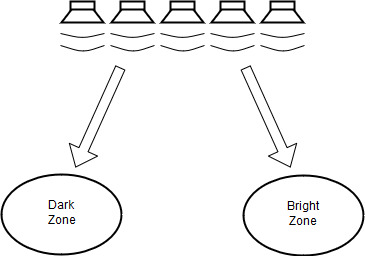
\includegraphics[width=10cm,height=10cm,keepaspectratio]{Figures/concept}
\decoRule
\caption[concept]{Overall concept. The idea is to use a set of loudspeakers to generate a difference in sound pressure level in two areas, the dark zone (low sound pressure) and the bright zone (high sound pressure). }
\label{fig:concept}
\end{figure}

In order to limit the disturbances created by said reflections, while developing an ACC method capable of acting on two soundzones, some experiments have been made, using an anechoic room as surrounding environment. This is a room specifically designed to dampen external sounds, as well as dramatically limiting the energy reflected back by the internal walls.
\\
There will necessarily be a divergence between the signal that has been inputted to the loudspeakers and the soundwave recorded by the microphones, this is due, mainly, to two different phenomena. The presence of reflections inside the room (that act as noise, as we said) and the nonlinear behavior of the loudspeakers. Any speaker, when solicited with a signal, will produce some unwanted sound components, that were not present in the original input.
\\
The impulse response (IR) is the figure that represents how the system (room, loudspeakers, other reflector surfaces) responds to said solicitations. It is derived by dividing the output of the system with its input. We will later see how the IR can be calculated for the specific system under test.
\\
\\
Going back to the ACC problem, this study analyses the feasibility of the approaches by the literature \parencite{cai_time-domain_2014,choi_generation_2002}, reproduces their results and proposes an evolution of the algorithm of choice that reduces the computational time required to find a filter(a set of weights) capable of generating some acoustic contrast. This is done in a specifically tailored scenario and with some limitations. The modified algorithm shows little degradation on the contrast figure with respect to the original solution proposed by \parencite{cai_time-domain_2014}. By measuring the impulse response and analyzing its characteristics it is possible to isolate the elements of the system that negatively affect the contrast (like reflective surfaces) and develop a filter that is able to limit their detrimental effect. This is achieved by splitting the impulse response (IR), the function that describes the characteristics of the room in question, in parts and creating an acoustic contrast filter for each one of these pieces, separately.
\\
\\
The scenarios used in the experiments will be progressively more difficult to control, since we will move from a simulated environment, to a real one, where it will be, at some point, added a reflective surface.
\\
The simulation will only consider two kinds of points, the ones that generate sound (which simulate some loudspeakers) and control points (which simulate some microphones), the physical implications of such objects will not be part of the experiment. Moving into the chamber, at the beginning, there will only be the necessary instruments to perform the experiments, namely the loudspeakers, used to reproduce the sound and the microphones, used to record the results of the experiments, together with the microphones power amplifiers. At a second time, a panel will also added inside the room, with the purpose of introducing a surface able to reflect sound. Before performing the ACC in the anechoic chamber some considerations about the speakers characteristics are made with a specifically designed experiment that analyses how different the sound signal, recorded by the microphones, is different with respect to the original one sent to them.
\\
In the end, the experiments will be repeated in a listening room, which is an environment much more similar to the living room of a common house, with tables, chairs, bookcases and other furniture. Needless to say, all of these objects will provide plenty of surfaces, that scatter sounds all over the room.
\\
\\
Summing up, the three scenarios where the ACC algorithm will be run are

\begin{enumerate}
  \item An anechoic chamber with the experiments hardware. 
  \item An anechoic chamber with the experiments hardware and a single reflective surface.
  \item A listening room with numerous surfaces that scatter sounds.
\end{enumerate}

The new technique devised in this work employs two ACC filters, developed using the same algorithm. These filters will tackle the problem of achieving contrast from two different sides, the first one will limit the acoustic energy in the dark zone coming \textbf{directly} from the loudspeakers.
\\
The second one will be applied in correspondence of the biggest source of reflections, which, in the case of point 2 of the above list, is also the only one having a clear and noticeable effect inside the room, while in point 3 the one taken into consideration and considered the "main" reflection will be one of the many present in the room.
\\
\\
The choice of having a maximum of two filters was not determined by some limitation in the algorithm, but rather dictated by a strive for consistency in the results, since there was a single surface in the anechoic chamber, a single reflection will be actively identified (and contrasted) in the listening room. Another problem, that will be discussed in chapter \ref{Chapter4} is that, while the reflection source is easily identifiable (and then separable) in the IR of the system in the anechoic chamber, it is not so easy to do so in the listening room. The windowing algorithm is discussed in section \ref{subsec:filtersplit}.
\\
Producing two different filters (one for the direct soundwave and one for the reflected one) takes much less computational time than calculating one single filter, which needs to be somewhat longer in order to be effective. Having a longer filter means that more samples of the IR are taken into account when calculating the ACC solution. The two shorter ones instead, can be merged and played back by the speakers, acting effectively in a similar manner as the longer one, but with a lower associated computational cost. This will necessarily introduce a decrease in the contrast figure, the magnitude of such trade-offs will be investigated in section \ref{subsec:filtersplit}.
\\
\\
The thesis objective can be overall synthesized as:
\\
\textbf{studying the ACC problem, focusing on the reflection problem, which is generated by having an object in the test environment that negatively impacts on the contrast achievable. This is done in a simplified scenario}.
\\
The solution proposed is then tested a listening room, where the validity of the concept is studied in a real-world scenario.
\\
\\
This work does not propose a definitive solution of the reflections problem, but takes a first step towards the resolution of the current limitations in the ACC algorithm chosen.
\\
The next few chapters will explain the specifics of the process, but at a glance, the work done can be summarized as follows,
\begin{itemize}
\item An algorithm able to perform ACC in wideband is selected. The algorithm was already available in literature \parencite{cai_time-domain_2014}. The proposed solution is reproduced.
\item The algorithm's performance is evaluated when changing some of its defining parameters (more details in \ref{sec:acc}).
\item The algorithm's limitations are analyzed. A variation that is capable to overcome at least some of its shortcomings is devised.
\item The modified version of the algorithm is tested, in some proposed use cases.
\end{itemize}

The following sections will describe the process carried out during the $4^{th}$ semester of the M.Sc. program at Aarhus University. The facilities used for this project were kindly made available by the Department of Engineering.

\section{Thesis structure}

In chapter \ref{Chapter2} the required theoretical background is presented to the reader. In section \ref{subsec:greenfct} is explained the propagation model that is the most popular for representing soundwaves moving in a spherical field. Later it is explained how a sound is generated by a loudspeaker and why its behaviour diverges from the ideal, linear case, by showing nonlinear distortions. In the end it is explained what ACC methods are and how do they work.
\\
\\
The experimental setup is described in details in chapter \ref{Chapter3}. In the chapter there are four sections that will explain the software, the hardware, the simulated and real environments used for the demonstrations. A detailed schema of the signal chain is presented in section \ref{subsec:sigchain}, that is how the digital, computer generated signal, arrives is reproduced and then recorded again by the microphones to be then converted back in a digital format. The power amplifiers, loudspeakers, microphones models and room dimensions are also listed in section \ref{sec:hw}.
\\
\\
Chapter \ref{Chapter4} analyzes the experiments in great detail, discusses and compares the results. Those are presented in progression as they have been performed, during the developing phase of this thesis work, in particular, the chapter is divided in experiments performed in the anechoic chamber (section \ref{sec:baccrd}) and the one made in the listening room (section \ref{sec:baccrdlisteningroom}). While progressing though them, the choices and trade-offs of the algorithm are investigated.
\\
\\
Finally, in chapter \ref{Chapter5} redacts the conclusions. It is there expressed what can be summarized from this work and where the main limitations lay. Moreover, a list of future improvements is proposed. 

% Chapter 2

\chapter{Background and Theory} % Main chapter title

\label{Chapter2} % For referencing the chapter elsewhere, use \ref{Chapter2} 

%----------------------------------------------------------------------------------------


\section{Sound Propagation}

In order to study the concept behind acoustic contrast control we first need to understand how the sound propagates from the speakers to the control points. The theoretical model that sets the stage is the Green's function. This function models the propagation of a soundwave of a system through a linear differential equation. Being an ideal model, it is a good approximation only in certain scenarios, this is because it can only describe a soundwave using a spherical field. This, while true at lower frequencies, it's not the real behavior of a wave once reached a certain critical frequency. What happens is that the propagation pattern is not spherical anymore, but start becoming multi-lobed, this particular shape is called cardioid. In the following figure we can see an example of this phenomenon. The propagation pattern (and the critical frequency) varies wildly between different loudspeaker models, the figure shows the behavior of a specific model, nevertheless, it can give the reader an idea on how the sound at different frequencies can propagate from a speaker.

\begin{figure}[th]
\centering
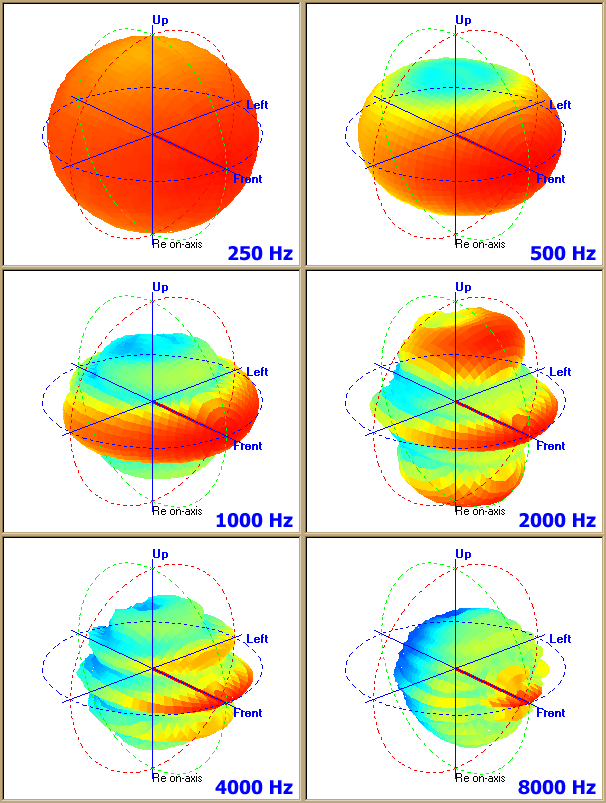
\includegraphics[width=8cm,height=9cm,keepaspectratio]{Figures/directivity}
\decoRule
\caption[Propagation pattern]{Propagation pattern of a loudspeaker at various frequencies. The speaker model is a Bosch 36 watt LA1-UW36-x. The figure is taken from on-line resources.}
\label{fig:directivity}
\end{figure}

We will use the Green's function for the very first part of the implementation of the acoustic contrast control algorithm, when testing it in a simulated scenario.

\subsection{Green's function}{}
\label{subsec:greenfct}

Resolving the sound propagation problem can be reduced to finding the appropriate weights to a matrix that correlates the wave origin points with the detection points. An easy and widespread way of solving the problem in the literature is by using the Green's function \parencite{elliott_robustness_2012,kuttruff_room_2014,shin_maximization_2010}.
\\
This function proposes a solution to a system of non-homogeneous differential equations. By finding the solution to said system it is possible to correlate the acoustic energy detected in a certain point in space with a linear combination of origin point sources. This relationship is linearly dependent from the distance of said point from the individual sound sources, multiplied the air resistivity.
\\
\\
Let's give an operative definition of the Green function by expressing the easiest boundary value problem for a differential operator, by saying

\[ L u = f,\quad u(a)=u(b)=0 \]

(it is reminded to the reader that since we're talking about a differential equation here $f$ is a function and $u(a), u(b)$ are boundary values), where $L = \frac{-d^2}{dx^2}$ is the second order derivative operator, in this case the Green function can be expressed by using $ - G'' = \delta (x - \xi)$, resolving $u$ then becomes equal to finding

\[ u=\int_{a}^{b} G(x,\xi)f(\xi)d\xi\]
where $f(\xi)$ is the value of the function in the point 
$ a \le \xi \le b $, and
\\
$G(x,\xi) = - \rho(x - \xi) + Ax + B$ is the Green's function, the result of the integration of $-G''$, $\rho$ is the ramp function ( the ramp function is the double integral of the delta function).
\\
\\
This means that it is possible to calculate the value that a differential equation takes in a certain point by knowing its input, the propagation function and some boundary values, this is conceptually not dissimilar of solving a linear system $Ax=y$, where instead of linear equation we have differential equations.
\\
Expanding on this concept it is possible to define a system of differential equations, where instead of a single source point it possible to calculate the effect that a linear combination of sources have in a determined point (in other words, the solution of the system).
\\
\\
This is very significant, because by knowing the Green's function (which is our theoretical model) of a soundwave, we can correlate the effect (having some acoustic energy in a point in space) with having a cause (a single, or even multiple sound sources, by the principle of superposition) and viceversa, that is, knowing how much does a source effect the total energy figure in a destination point.
\\
\\
The Green equation for a sound field is \parencite{elliott_robustness_2012,kuttruff_room_2014,shin_maximization_2010}:

\begin{equation}
G(r)=-j \rho 2 \pi f \frac{e^{-j k r}}{4 \pi r};
\label{eqn:green}
\end{equation}

Where $j$ is the imaginary unit, $\rho$ is the atmospheric air density. $\rho = 1.21$ is the air density value at sea level and at $15^{\circ}$C, $k$ is called the wave number and is equal to $k = \frac{2 \pi}{\lambda}$ with $\lambda$ as the wavelength and $r$ is the distance (radius) between source and destination. 
\\
\\
Unfortunately the solution of the Green's function exist in closed form only in some simple cases. In order to determine how a soundwave propagates in a more complex space (such the one of an anechoic chamber or a listening room) it is necessary to directly measure the output of a speaker and correlate it with the input used as solicitation.
\\
One more problem to consider is the one regarding the assumption of having a spherical propagation pattern. Unfortunately this kind of behavior is true for soundwaves having a relatively low frequency, in fact, by increasing the sound frequency the real world scenario grows more distant to the ideal one, the spherical pattern tends to resemble a multi-lobed one. The critical frequency, shape and number of the lobes depend on the dimensions, power, construction material, shape of the speaker cone and can be described only on a case by case basis.


\section{Sound generation and harmonics}
\label{sec:soundgen}

The sound actuator, or loudspeaker, is an electromagnetic device that uses a rapidly changing electrical bipole, generated by a coil glued on a cone-shaped cloth or silicate, usually made of copper, to generate movement through the interaction of the resulting magnetic field (as described by the Ampere-Maxwell laws), with a permanent or semi-permanent magnet situated behind the moving coil.
\\
\begin{figure}[th]
\centering
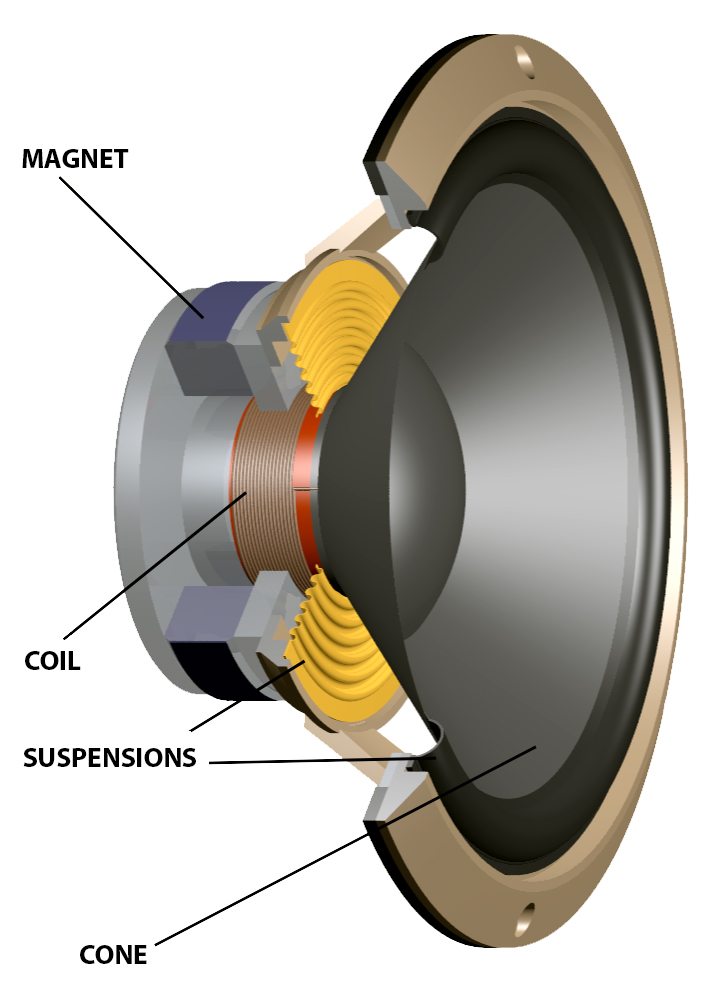
\includegraphics[width=7cm,height=7cm,keepaspectratio]{Figures/loudspeaker}
\decoRule
\caption[Loudspeaker representation]{Cut-out of a generic loudspeaker, here the reader can recognize the main elements. The figure is taken from on-line resources and modified.}
\label{fig:loudspeaker}
\end{figure}

The kind of behavior that a loudspeaker shows changes at low and high amplitudes. This dependency from the amplitude is non linear. As a consequence of this nonlinearity we have that in response to a stimuli signal, some frequency components, non existent in the input, will appear. This components will show themselves at integer multiples of the input frequency, for instance, if the input is a $200$Hz sine-wave with a certain amplitude, in the frequency response of the system, some peaks (usually, but not always, with a smaller amplitude than the first one) will appear at $400$Hz, $600$Hz and so on. These components are called higher order harmonics.

\begin{figure}[th]
\centering
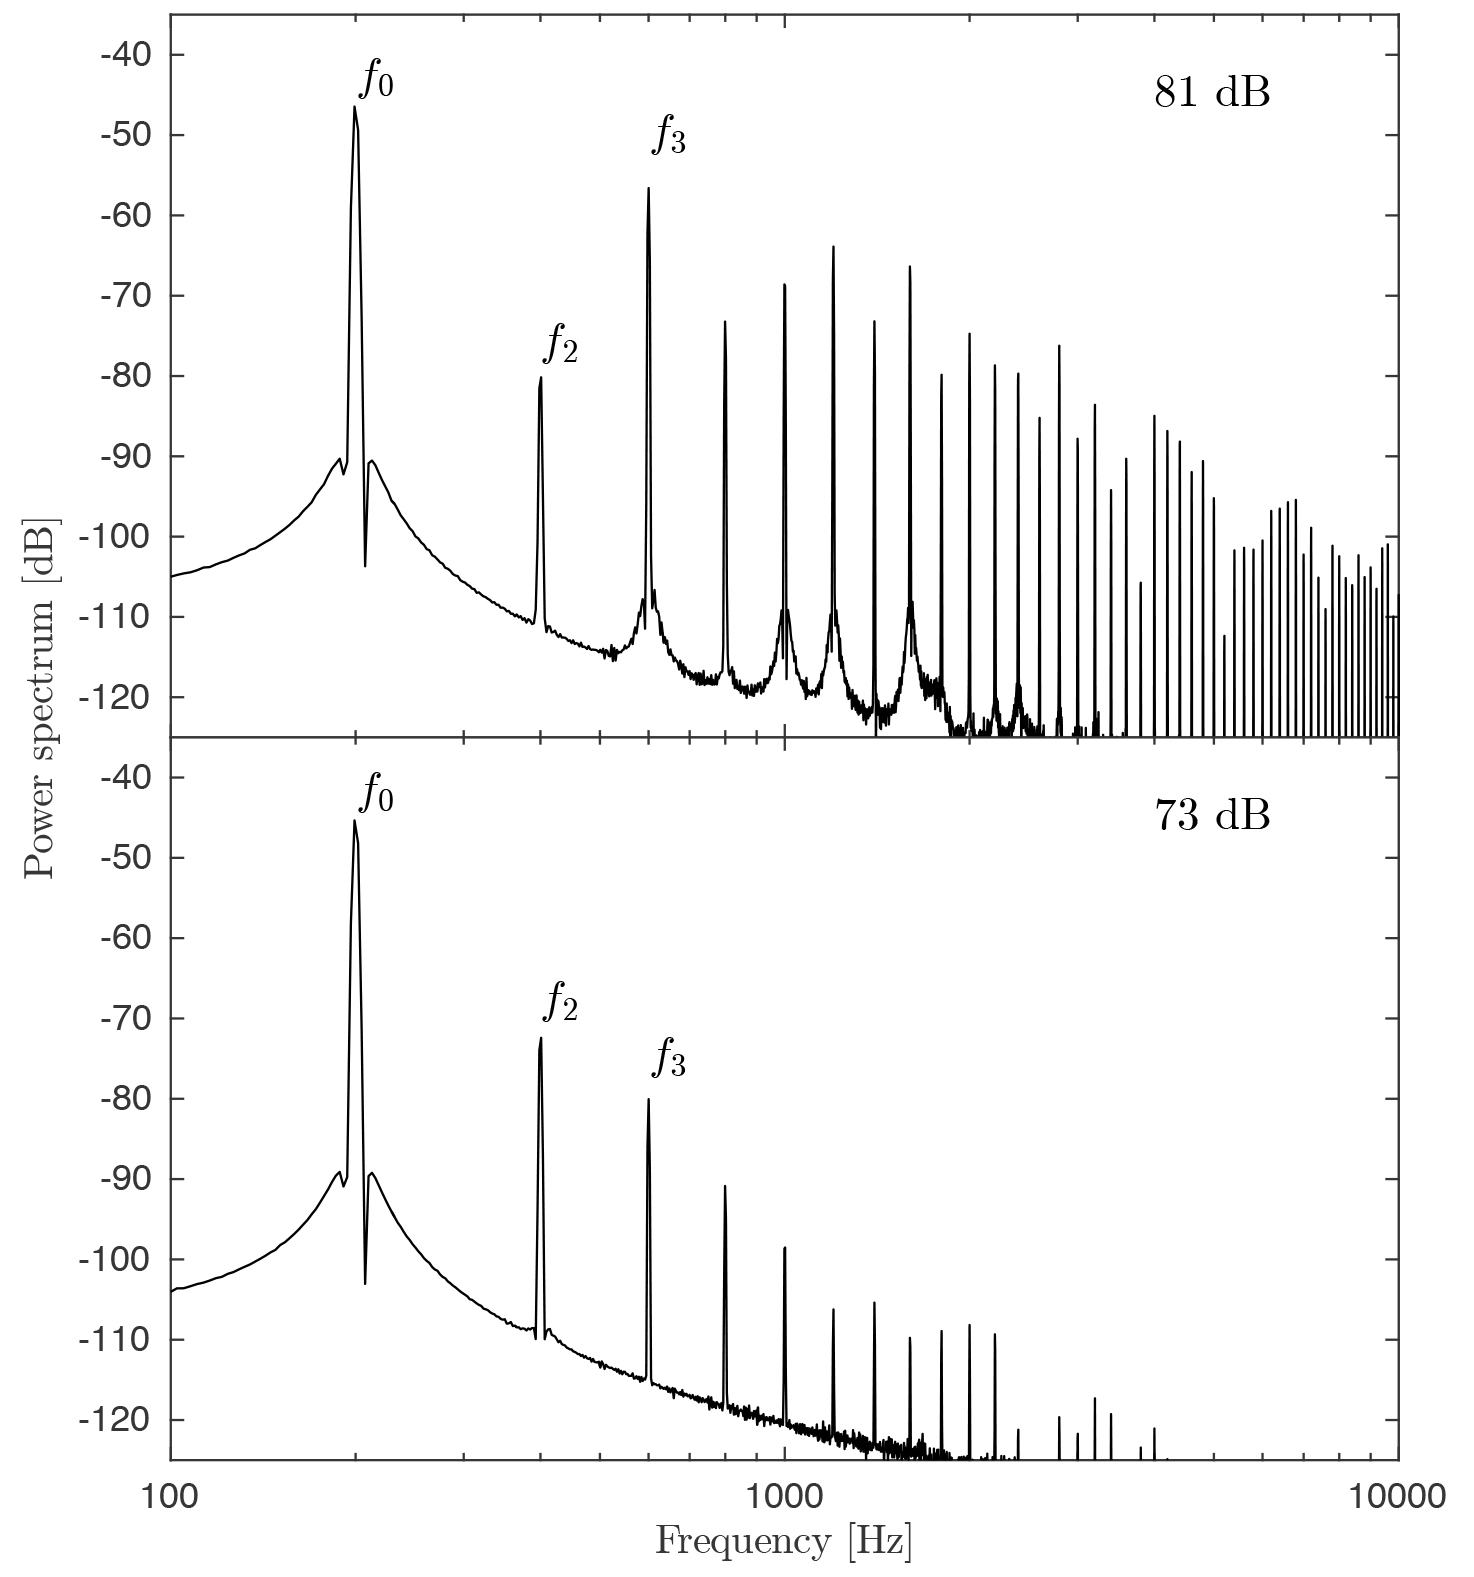
\includegraphics[width=9cm,height=10cm,keepaspectratio]{Figures/nonlinearities}
\decoRule
\caption[Frequency response of a loudspeaker emitting a sine wave at 200Hz]{Frequency response of a loudspeaker emitting a sine wave at 200Hz. The reader can notice the higher order harmonics at multiples of $200$Hz. Increasing the amplitude increases the presence of nonlinearities. Graph taken from \parencite{ma_personal_2016}.}
\label{fig:nonlinearities}
\end{figure}
We can also see from the figure that playing at high amplitudes generates even more non linearities, this is because the cone displacement increases, so the force applied on the coil varies more \parencite{ma_personal_2016}.
\\
\\
Additionally, if the input signal has significant components at more than one single frequency, these will interfere with each other, generating a phenomenon known as inter-modulation distortion, the interaction between these components will form additional signals at frequencies that are not just at integer multiples of said components, but also at the sum and difference frequencies of the original ones. This generates a cascade of unwanted components that interact with each other and generally degrade the signal-to-noise ratio of the system.
\\
\\
The nonlinear behavior showed by a loudspeaker at low amplitudes is given by the fact that the stiffness of the cone is not constant for varying amount of force exerted, this means that the displacement is different from the one intended, in other words the mechanical characteristics of the component (mainly the cone) constituting the speaker deviate from the expected behavior.
\\
High amplitudes tend to accentuate the imperfections in the driver unit, for instance, local changes in the rigidity of the cone, or misplacement of the glue that holds the cone to the frame. Moreover, the displacement in the two directions (front/back) is not equal, mainly because the mechanical impedance is not equal in the two directions. Also, the force that couples the mechanical and electrical side of the speaker is not constant. We can describe this force as the integral of the magnetic flux density $B$, versus voice coil wire length $l$. We can plot the force factor $Bl(x)$ and see that it is not a constant, but it depends on the displacement $x$ of the coil. More distant is the coil from the magnet, less force it will experience \parencite{klippel_tutorial:_2006}.

\begin{figure}[th]
\centering
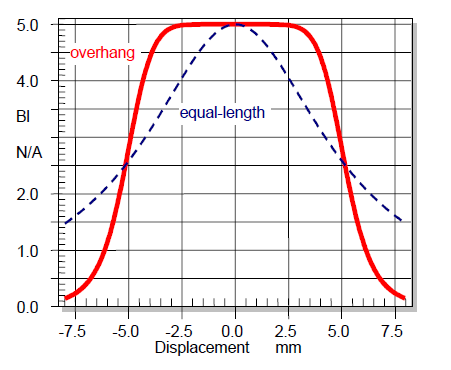
\includegraphics[width=8cm,height=8cm,keepaspectratio]{Figures/displacement}
\decoRule
\caption[Force factor vs. displacement]{Plot of the force experienced by the coil versus its displacement. Overhanging is a method to improve the performances, it consists in making length $l$ of the coil bigger than the section of the magnet, so that the magnetic flux is less dependent from the relative position of the cone. Graph taken from \parencite{klippel_tutorial:_2006}.}
%\label{fig:directivity}
\end{figure}

At low frequencies the main cause of nonlinearity is the big excursion of the coil. This causes a big variation in the magnetic field, which exerts a smaller force when the coil is distant from the magnet.
\\
At high frequencies, the rapid movement of the cone strains the materials, that start showing different properties from the expected ones, these phenomena are known as break-up modes. At higher frequencies the cone starts to bend, instead of moving as a whole generating resonance effects, this happens at fixed frequencies that are not related to the input signal.
\\
\\
As we've just discussed, a speaker shows nonlinear behavior when excited in ranges close to its operational limits. The intensity of the nonlinearities generated is not the same for all of these critical modes. As already seen in figure \ref{fig:nonlinearities}, the worst scenario is when the speaker is excited at high amplitudes and low frequencies.
\\
\\
The presence of nonlinearities is detrimental to the performance of the acoustic contrast filter we will calculate, since it reduces the contrast figure achievable, this is because of two reasons.
\\
First, as previously stated, the distortions are parts of the output signal that weren't present in the original one, they act essentially as noise, therefore compromise the contrast figure.
\\
Second, the model used in the algorithms that implement the ACC method only treats the linear part of the system. In principle it is possible to define a more complex model that takes into account the higher harmonics, but developing such a model is beyond the scope of this project. Even though this is a big issue of the current control methods available, this problem has been avoided during this work, by choosing an appropriate frequency range and playing at low enough amplitudes, so that their generation is not too evident.

\section{Acoustic Contrast Control}
\label{sec:acc}

The first description of an Acoustic Contrast Control (ACC) algorithm was given in 2002 \parencite{choi_generation_2002}. Since then, different contributors in the academia have proposed new solutions that refine the concept \parencite{elliott_robustness_2012,cai_time-domain_2014}, in this section we will discuss the principles that guide these algorithms and some important aspects that have been considered for choosing the appropriate one for this thesis work.
\\
\\
The main principle of ACC is to reproduce a soundwave that has the same intensity (amplitude) and opposite phase with respect with another soundwave that we do not wish to have. When these waves meet they cancel each other out. This is intuitively simple to understand, since the propagation of a soundwave can be expressed as a portion of space where air particles get compressed or expanded as the wave passes by, the amount of compression (or expansion) depends on the intensity of the wave, the kind of adiabatic transformation (compression or expansion) depends on its phase and the direction depends on the position of the source. If two equally ample, but opposite fluxes of air meet with exactly the opposite phase, they will destructively interfere with each other. For the same reason, two fluxes with the same phase will add to each other, and every result in between this two cases will lead to an increase or decrease of the resulting flux, depending on the relative phase difference of the two waves.
\\
\\
This simple principle has led to the development of active noise control (ANC), a control method that is relatively widespread that appears in many consumer-grade electronics, especially headphones and earplug.
\\
ACC is fundamentally different than ANC. While the implementation of ANC can be relatively inexpensive, mostly because the signal and the noise are well distinct (in principle, everything coming from the external world is treated as noise), and since the sound sources are close the ear canal of the user the power required to cancel the undesired sources is very limited. With ACC instead, two signals can coexist in the same space, and there is no clear distinction between what is the signal and what is the noise by itself, but those term acquire now a local significance, meaning that a particular sound might be considered noise only in a limited region of space. The fact that more sounds have to share the same channel introduces a new set of constraints, for instance, adding acoustical energy to the environment (by increasing the control effort) is not necessarily the best course of actions to increase the contrast figure.
\\
As explained in section \ref{sec:soundgen}, high amplitude sounds generate higher harmonics that are very difficult to control, sound propagation pattern diverges from the spherical formulation described by subsection \ref{subsec:greenfct} and also the room acoustics now become a factor to consider when designing the algorithms. Tackling these issues has required 15 years of research and many more years will probably be necessary before seeing the adoption of this technologies by the industry for mainstream consumer market.
\\
\\
Going back to the specifics of the ACC, it is conceptually equivalent to have two different sound signals that have to be addressed to two different zones, or having a single signal that has to be reproduced in a zone, while suppressed in another one. In all sections of this work, the second case will be the one treated.
\\
\\
Let's now give a mathematical definition to ACC, let's start by defining the acoustic energy $e_b$.
\\
For a volume $V_b$, the acoustic energy is defined as

\begin{equation}
e_b=\frac{1}{V_b}\int_{V_b}p(\vec{x}) p(\vec{x}) dV
\label{eqn:acousticenergy}
\end{equation}

please note that $b$ refers to the bright zone, the formulation for the dark zone is identical. $p(\vec{x})$ is the sound pressure, that can be expressed \parencite{choi_generation_2002} as

\begin{equation}
p(\vec{x})=\sum\limits_{i=1}^K \textit{G}(\vec{x}|\vec{x}_c^{(i)})q_c(\vec{x}_c^{(i)}) = G(\vec{x}|\vec{x}_c)q_c
\label{eqn:soundpressure}
\end{equation}

where $K$ is the total number of sources available, $\textit{G}(\vec{x}|\vec{x}_c^{(i)})$ is the propagation function (the Green's function described in section~\ref{subsec:greenfct}) between the position $\vec{x}$ and the control source position $\vec{x}_c^{(i)}$ of loudspeaker $i$ (where $i=1...K$) and $q_c$ is the volume velocity, which measures the amount of air flowing in a given volume, per unit of time.
\\
\\
The energy can also be expressed by calculating the square of the complex magnitude of the pressure

\begin{equation}
\label{eqn:energycorrelationformulation}
\vec{e_b}=\frac{1}{V_b}\int_{V_b}p(\vec{x}) * p(\vec{x}) dV = q_c^H\left(\frac{1}{V_b}\int_{V_b} \textit{G}^H(\vec{x}|\vec{x}_c)\textit{G}(\vec{x}|\vec{x}_c) dV\right)q_c = q_c^H R_b q_c
\end{equation}

where $R_b$ represents the spatial correlation of the pressure field in the bright zone produced by each control source \parencite{choi_generation_2002}.
This will prove especially useful later, because, while the propagation (Green's) function cannot be expressed in a real experimental scenario, it's relatively easy to calculate the correlation figure, in particular, the acoustic contrast can be defined \parencite{cai_design_2013}, as the ratio of

\begin{equation}
\delta=\frac{e_b}{e_d}=\frac{w^T R_b w}{w^T R_d w}
\label{eqn:contrast}
\end{equation}

Where $w$ is a set of weights derived from the ACC algorithm explained below, while $R_b(n), R_d(n)$ refer to the $n$th control point, either in the bright or dark zone. This spacial dependence is implicit in defining the correlation, therefore omitted from this point forward.
\\
It appears clear that the maximization of such ratio can be achieved in two ways: maximizing the energy in the bright zone, or maximizing the ratio between total energy and energy in the bright zone. In both cases, finding the optimum set of weights, corresponds to find the solution to a Lagrange optimization problem.
\\
\\
Let's consider the first case, the output power can be written as a function of the volume velocity as $J_0=q_c^H q_c$ \parencite{choi_generation_2002}, the problem can now be formulated as constrained optimization problem under the form
\\
\[ \begin{aligned}
&\text{maximize} \quad
&& e_b=q_c^H R_b q_c
&\\
&\text{subject to} \quad 
&& J_0=q_c^H q_c
\end{aligned} \]
\\
which, introducing the Lagrange multiplier $\alpha$ can be written in a single equation as
\[\begin{aligned}
&\text{maximize} \quad J=q_c^H R_b q_c + \alpha(J_0-q_c^Hq_c)
\end{aligned}\]

taking the partial derivatives $\frac{\delta}{\delta q_c}$ and $\frac{\delta}{\delta \alpha}$ and solving the resulting system for $\alpha$ \parencite{choi_generation_2002,elliott_robustness_2012}, we get

\begin{equation}
\label{eqn:alpha}
\alpha=\frac{e_b}{J_0}=\frac{q_c^H R_b q_c}{q_c^Hq_c}
\end{equation}
\\
The acoustic contrast is maximized when the volume velocity $q_c$ is highest. Finding this maximum value is equivalent to find the solution to the generalized eigenvalue problem written as $\lambda q_c=A q_c$; $q_c$ can be treated as an eigenvector that has its maximum when it's equal to the maximum eigenvalue of $R_b$. The solution can be written as $q_{max} = \frac{\sqrt[]{J_0}}{\alpha} R_b^H$. In simpler terms, when the correlation, times a function that somehow describes the characteristics of the channel, is maximized, we have the maximum acoustic contrast
\parencite{shin_maximization_2010,choi_generation_2002}.
\\
\\
This formulation is not the most convenient one, because, while we maximize the energy in the bright zone, it doesn't take into account the energy that is being outputted in the dark zone, this can generate a relatively "loud" area, even in the dark zone. Moreover, as already explained, outputting higher powers generates non linearities in the speakers, which is highly undesirable, since it can further reduce the contrast, and more generally, create sound artifacts that impact negatively on the user experience. There is also a physical limit on the maximum power achievable given by the specific hardware (amplifiers, loudspeakers) that are being used.
\\
\\
The second method takes into account the enrgy in both zones and tries to maximize the contrast by tuning the output energy making sure that a minimum amount "leaks" into the dark zone. The Lagrange parameter adds flexibility to the algorithm, meaning that having a large $\alpha$ generates more energy in the bright zone. The increase in sound intensity in this zone is more beneficial (gives more contrast) than keeping a lower energy level, vice versa, a smaller $\alpha$ means that in order to get the best result is best to limit the output power. 
\\
The optimization function can be written as
\begin{equation}
\label{eqn:beta}
\beta=\frac{e_b}{e_t}=\frac{q_c^H R_b q_c}{q_c^H R_t q_c}, \quad e_t = e_b + e_d, \quad R_t = R_b + R_d
\end{equation}
\\
The cost function can be calculated in the same manner
as the maximization method, the maximum is obtained from the eigenvector of $R_t^{-1} R_b = \beta_{max}$ corresponding to the largest eigenvalue of the matrix \parencite{choi_generation_2002,schellekens_time_2016}. This, once convolved with the output signal, will generate acoustic contrast.
\\
Both the approaches discussed above are frequency dependent, meaning that a control frequency is defined in the algorithm and the optimization problem is then applied to it.
\\
\\
Looking closely at the equations \ref{eqn:beta} and its solution, it is possible to notice a fundamental problem, first treated by \parencite{elliott_robustness_2012}, that is, sometimes there can be numerical problems related to the correlation matrices, equation \ref{eqn:energycorrelationformulation} says that $R_b =\textit{G}^H(\vec{x}|\vec{x}_c)\textit{G}(\vec{x}|\vec{x}_c)$, in order to be invertible, has to be full rank. It might happen that $R_t$ is singular, or non-invertible (remember that $ R_t = R_b + R_d$).
\\
\parencite{elliott_robustness_2012} introduced a regularization term to improve on the robustness of the algorithm. The problem with having a frequency domain formulation is that the response of the filter is controlled only at determined frequencies, in particular, these algorithm chooses a control frequency (the one that leads to the maximum contrast) and increase its output power. This can lead to wild variations of the response at non-control frequencies and, in general a noticeable distortion of the FR in the bright zone.
\\
\\
In order to solve this controllability problem, \parencite{cai_time-domain_2014} have created two methods that provide contrast, while controlling the frequency response in the bright zone, in a broad range of frequencies. These methods are called Broadband Acoustic Contrast Control Response Variation (BACC-RV) and its later variation, Broadband Acoustic Contrast Control Response Differential (BACC-RD).
\\
These method have a fundamental difference with regard of the ones just described (though they have a similar formulation). That is, both are time domain resolved.
\\
All the frequency domain filters have to be brought in the time domain before being applied to the output sound signal (using the Inverse Fourier Transform). Moreover, in order to have a good frequency response, only a long filter can provide a good contrast over a broad spectrum of frequencies, condition that is not as fundamental in the time domain (even though in principle a longer filter it's always preferable, since it improves the contrast). This causes an unnecessary delay given by the domain conversion. Instead of measuring the frequency response and define a control frequency it is possible instead to work directly with the impulse response of the system.
\\
\\
Now that the reader has been given an overview of ACC fundamentals, it will appear more clear why BACC-RV/RD have been the method considered for the development of the core algorithms of this work, and the starting point for the modifications proposed in later sections (Chapter \ref{Chapter4}). The RD method has been preferred over the RV one because, even though it has very similar performances \parencite{cai_time-domain_2014,schellekens_time_2016}, it only has 2 tuning parameters instead of 3.
\\
\\
The formulation of the eigenvalue problem for the BACC-RD algorithm, solved using the Lagrange multipliers problem is expressed as

\begin{equation}
L = \frac{w^T R_b w}{\beta w^T R_d w + (1 - \beta) RD + \delta w^T w}
\label{eqn:lagrange}
\end{equation}
Where $\beta$ is a weight factor, setting the trade-off between the acoustic contrast and the flatness of the frequency response in the bright zone in the frequency range of interest, $0\le \beta \le 1$. $\delta$ is the regularization term, introduced by \parencite{elliott_robustness_2012}, it ensures robustness against statistical outliers in the noise figure, defining a maximum deviation that is allowed in the correlation to its mean square value. $R_b, R_d$ are the correlation matrices in the bright and dark zones and $w$ is a vector of weights, which maximization will eventually generate the contrast.
\\
\\
The optimum of the equation is deducted by maximizing $w$, it can be formulated by the expression
\\
\begin{equation}
w_{BACC} = \underset{w}{\operatorname{argmax}} \; L
\label{eqn:optimization}
\end{equation}

the solution of equation \ref{eqn:optimization} returns the BACC filter which generates the highest acoustic contrast. This is term corresponds to the largest eigenvalue of the matrix
\\
\begin{equation}
\delta=\frac{e_b}{e_d}=\frac{w^T R_b w}{w^T R_d w}
\label{eqn:contrast}
\end{equation}\[ \left[ \beta RD + \frac{1 - \beta}{(J-1) K}\sum\limits_{k=1}^{K} \Re \{ (V S_k)^H (V S_k) \} + \delta U \right]^{-1} R_b\]
\\
Where $U$ is the identity matrix \parencite{cai_time-domain_2014}, $K$ is the number of control points available, which is where the microphones will be positioned for the experiments, $J$ is the number of control frequencies and $V$ and $S_k$ are two matrices, defined as

\[V=\begin{bmatrix}
    -1 & 1 & 0 & \dots & 0 & 0 \\
    0 & -1 & 1 & \dots & 0 & 0 \\
    \vdots & \vdots & \vdots & \ddots & \vdots \\
    0 & 0 & 0 & \dots & -1 & 1
	\end{bmatrix}, \quad
S_k= \begin{bmatrix}
    s_{k}^T(f_1) \\
    \vdots \\
    s_{k}^T(f_j)\\
    \vdots \\
    s_{k}^T(f_J)
	\end{bmatrix}
\]
The product $V S_k$ controls the points where the frequency response is optimized, which total number of these frequencies is $J$. $S_k$ is in reality $S_{bk}$ or $S_{dk}$, depending on which zone we are considering.
\\
The $V$ matrix effectively perform the differentiation of each of the $k$ output vectors $s_{k}(f)$. The control frequencies $f_j$ are the points where the contrast between the two zones will be maximized. The number of control points depends on the on the sampling frequency of the signal, while the space between them is affected by the length (in samples) of the filter. A longer filter allows for more closely spaced control frequencies (also called bins), this will increase the contrast figure.
\\
At first glance one can see that equation \ref{eqn:lagrange} is similar to the formulation \ref{eqn:contrast}, with the addition of the $RD$ term and two parameters, $\beta,\delta$ \parencite{cai_time-domain_2014}.
\\
The $RD$ term is described by

\begin{equation}
RD = \frac{1}{(J-1)K}\sum\limits_{k=1}^K (V S_k w)^H (V S_k w)
\label{eqn:RD}
\end{equation}
\\
The $S_k$ matrix is derived by Fourier transforming the output vector, which is the convolution between input signal, room impulse response and the filter vector $w$, assuming the input signal is a Dirac's delta function, it can also be written as (with the bright zone formulation)

\[S_{bk}=\mathcal{F}[y_{bk}(n)]=\mathcal{F}[w^T r_{bk}(n)]\]
\\
which is the product between the weight vector and the filtered impulse response of the system to the Dirac's delta, as generated by source point $k$ \parencite{cai_time-domain_2014}.
\\
The filtered vector $r_{bk}(n)$ is equal to

\[ r_{bk}(n) = [h_{b_1k}(n),\dots,h_{b_1k}(n-M+1),\dots\dots, h_{b_Lk}(n),\dots,h_{b_Lk}(n-M+1)]^T\]
\\
As we can see, it filters the impulse response between the source $l$ and the control point $k$ and has length $M$. 
The $b$ in the notation specifies that the control point is in the bright zone. The equivalent equation for the output vector $y_{dk}$ is described in the same way.
\\
\\
In the case the signal is wideband, we might wonder how the filtered vector can be described. The optimized frequency response $\rho_{bk}(f)$  can be written as

\begin{equation}
\rho_{bk}(f) = \sum\limits_{n=0}^{M+I-2} y_{bk}(n) e^{-j2\pi f n T_s}=w^T s_{bk}(f)=w^T [r_{bk}(n) e^{-j2\pi f n T_s}]
\label{eqn:freqresp}
\end{equation}

$y_{bk}$ is the output vector, also called the global response, it comprises the input, the filter weights $w$ and the room transfer function $h_{blk}$ between the loudspeaker $l$ and the control point $k$. It has length $M+I-1$.
$M$ and $I$ are the lengths of the weights vector and the system's impulse response (in the time domain). These values can be adjusted independently of each other. As we can see from this formulation, the control frequencies vector $S_k$ is multiplied with $w^T$, which weights the contribution that each frequency bin has to the (wideband) frequency response of the system. The spacing between bins depends on the length $M$ of the filter, a longer filter can more finely control the frequency response of the system.
\\
\\
The $RD$ term can be expressed in terms of the frequency response \parencite{cai_time-domain_2014,schellekens_time_2016}, with a formulation similar to the one of the mean square error

\begin{equation}
RD = \frac{1}{(J-1) K} \sum\limits_{k=1}^{K} \sum\limits_{j=1}^{J-1} |\rho_{bk}(f_{j+1}) - \rho_{bk}(f_j)|^2
\label{eqn:RDfreqresp}
\end{equation}

The smaller is this term, the flatter frequency response we will be able to achieve.

For consistency with equation~\ref{eqn:acousticenergy}, it can be said that \parencite{cai_time-domain_2014}
\[ y_{bk}(n)=w^T r_{bk}(n), \quad e_b=\sum\limits_{k=1}^{K}\sum\limits_{n=0}^{M+I-2}\frac{y_{bk}^2(n)}{K} = w^T R_b w\]
\\
As previously stated, an interesting property of the algorithm is that we have two parameters, $M$ and $I$, those are, respectively the IR length and the FIR filter length, we can arbitrarily decide to cut short the time-domain response of the room. This characteristic will prove extremely useful for the management of the computational resources available, since it will dramatically speed up the calculation of the $R_b$ and $R_d$ matrices.
\\
Moreover, having an adjustable filter length makes this kind of filter effective even at short lengths. Of course, the longer the impulse response of the system, the more we will be able to control the system. As we will see later, this also means increasing the number of operations necessary to calculate the filter, specifically, the correlation matrices $R_b, R_d$ increase with the square of the filter length, this for each microphone-speaker pair. As we will see in chapter ~\ref{Chapter4} this makes filters longer that 600 taps very impractical to calculate.

 
\chapter{Experimental Setup} % Main chapter title

\label{Chapter3} % For referencing the chapter elsewhere, use \ref{Chapter3} 

%----------------------------------------------------------------------------------------
\section{Software}
\subsection{Matlab, portaudio, playrec}{}
\label{subsec:matlab}

The main piece of software used to performed all the required measurements and experiments was Matlab, a graphical environment for the development of highly specialized and computationally intensive computer programs. Its proprietary programming language was used to design the algorithms subject of the thesis and to interact with the hardware used for the experiments, thanks to two third-party interfaces Portaudio and Playrec.
\\
In order to send the input signal to the DAC and subsequently to the Loudspeakers it was necessary to use some drivers that allowed for a low latency streaming on multiple channels. For this purpose the out-of-the-shelf package of choice were Portaudio, an open-source audio I/O library and Playrec, a middleware that builds on top of Portaudio and provides a very simple API to the Matlab environment allowing to perform non-blocking calls to the soundcard using the ASIO protocol, which allowed to satisfy the low latency communication requirements between the software and the soundcard hardware.
\\
The reason why Playrec's API were chosen among other candidates was that it allows for the simultaneous playback and recording of sound. This simplifies the IR estimation of the system. Making sure the starting sample is the same between playing and recording makes possible to have a good estimation of the acoustic delay, that is the time (expressed in number of samples) between the moment the speakers start playing, from the time the microphones start picking up the first samples of the signal.

\subsection{Logsweep signal}{}
\label{sec:logsweep}

In section \ref{subsec:greenfct} it was explained how the propagation of a soundwave can be approximated by using of the Green's Function. It was also explained that this model shows its limits when the frequency (and therefore the wavelength) of the sound signal is high enough so that the propagation field is not spherical anymore and the sound source cannot be considered as a point. Also, the presence of reflections complicates the propagation model so much, that the Green's function does not have a closed-form solution anymore and an experimental approach becomes by far the easiest way of estimating the system IR.
\\ 
In order to refine the IR estimation (which, as explained in section \ref{sec:intro} describes the characteristics of the room-speakers-microphones system), a new model is required. The function that allows for such a precise estimation is the Logsweep function, also called chirp tone.
\\
Suppose one wants to estimate the performance of a system using a sine wave. It is well known that the system response can be expressed by the formula
\begin{equation}
h(t) = \frac{y(t)}{x(t)}
\label{eqn:h}
\end{equation}

Where $x(t)$ is the input signal and $y(t)$ is the output. The frequency response of a real loudspeaker system, excited with a sine wave at a specific frequency ($200$Hz), that is obtained by Fourier transforming $h(t)$ looks similar to 
\begin{figure}[th]
\centering
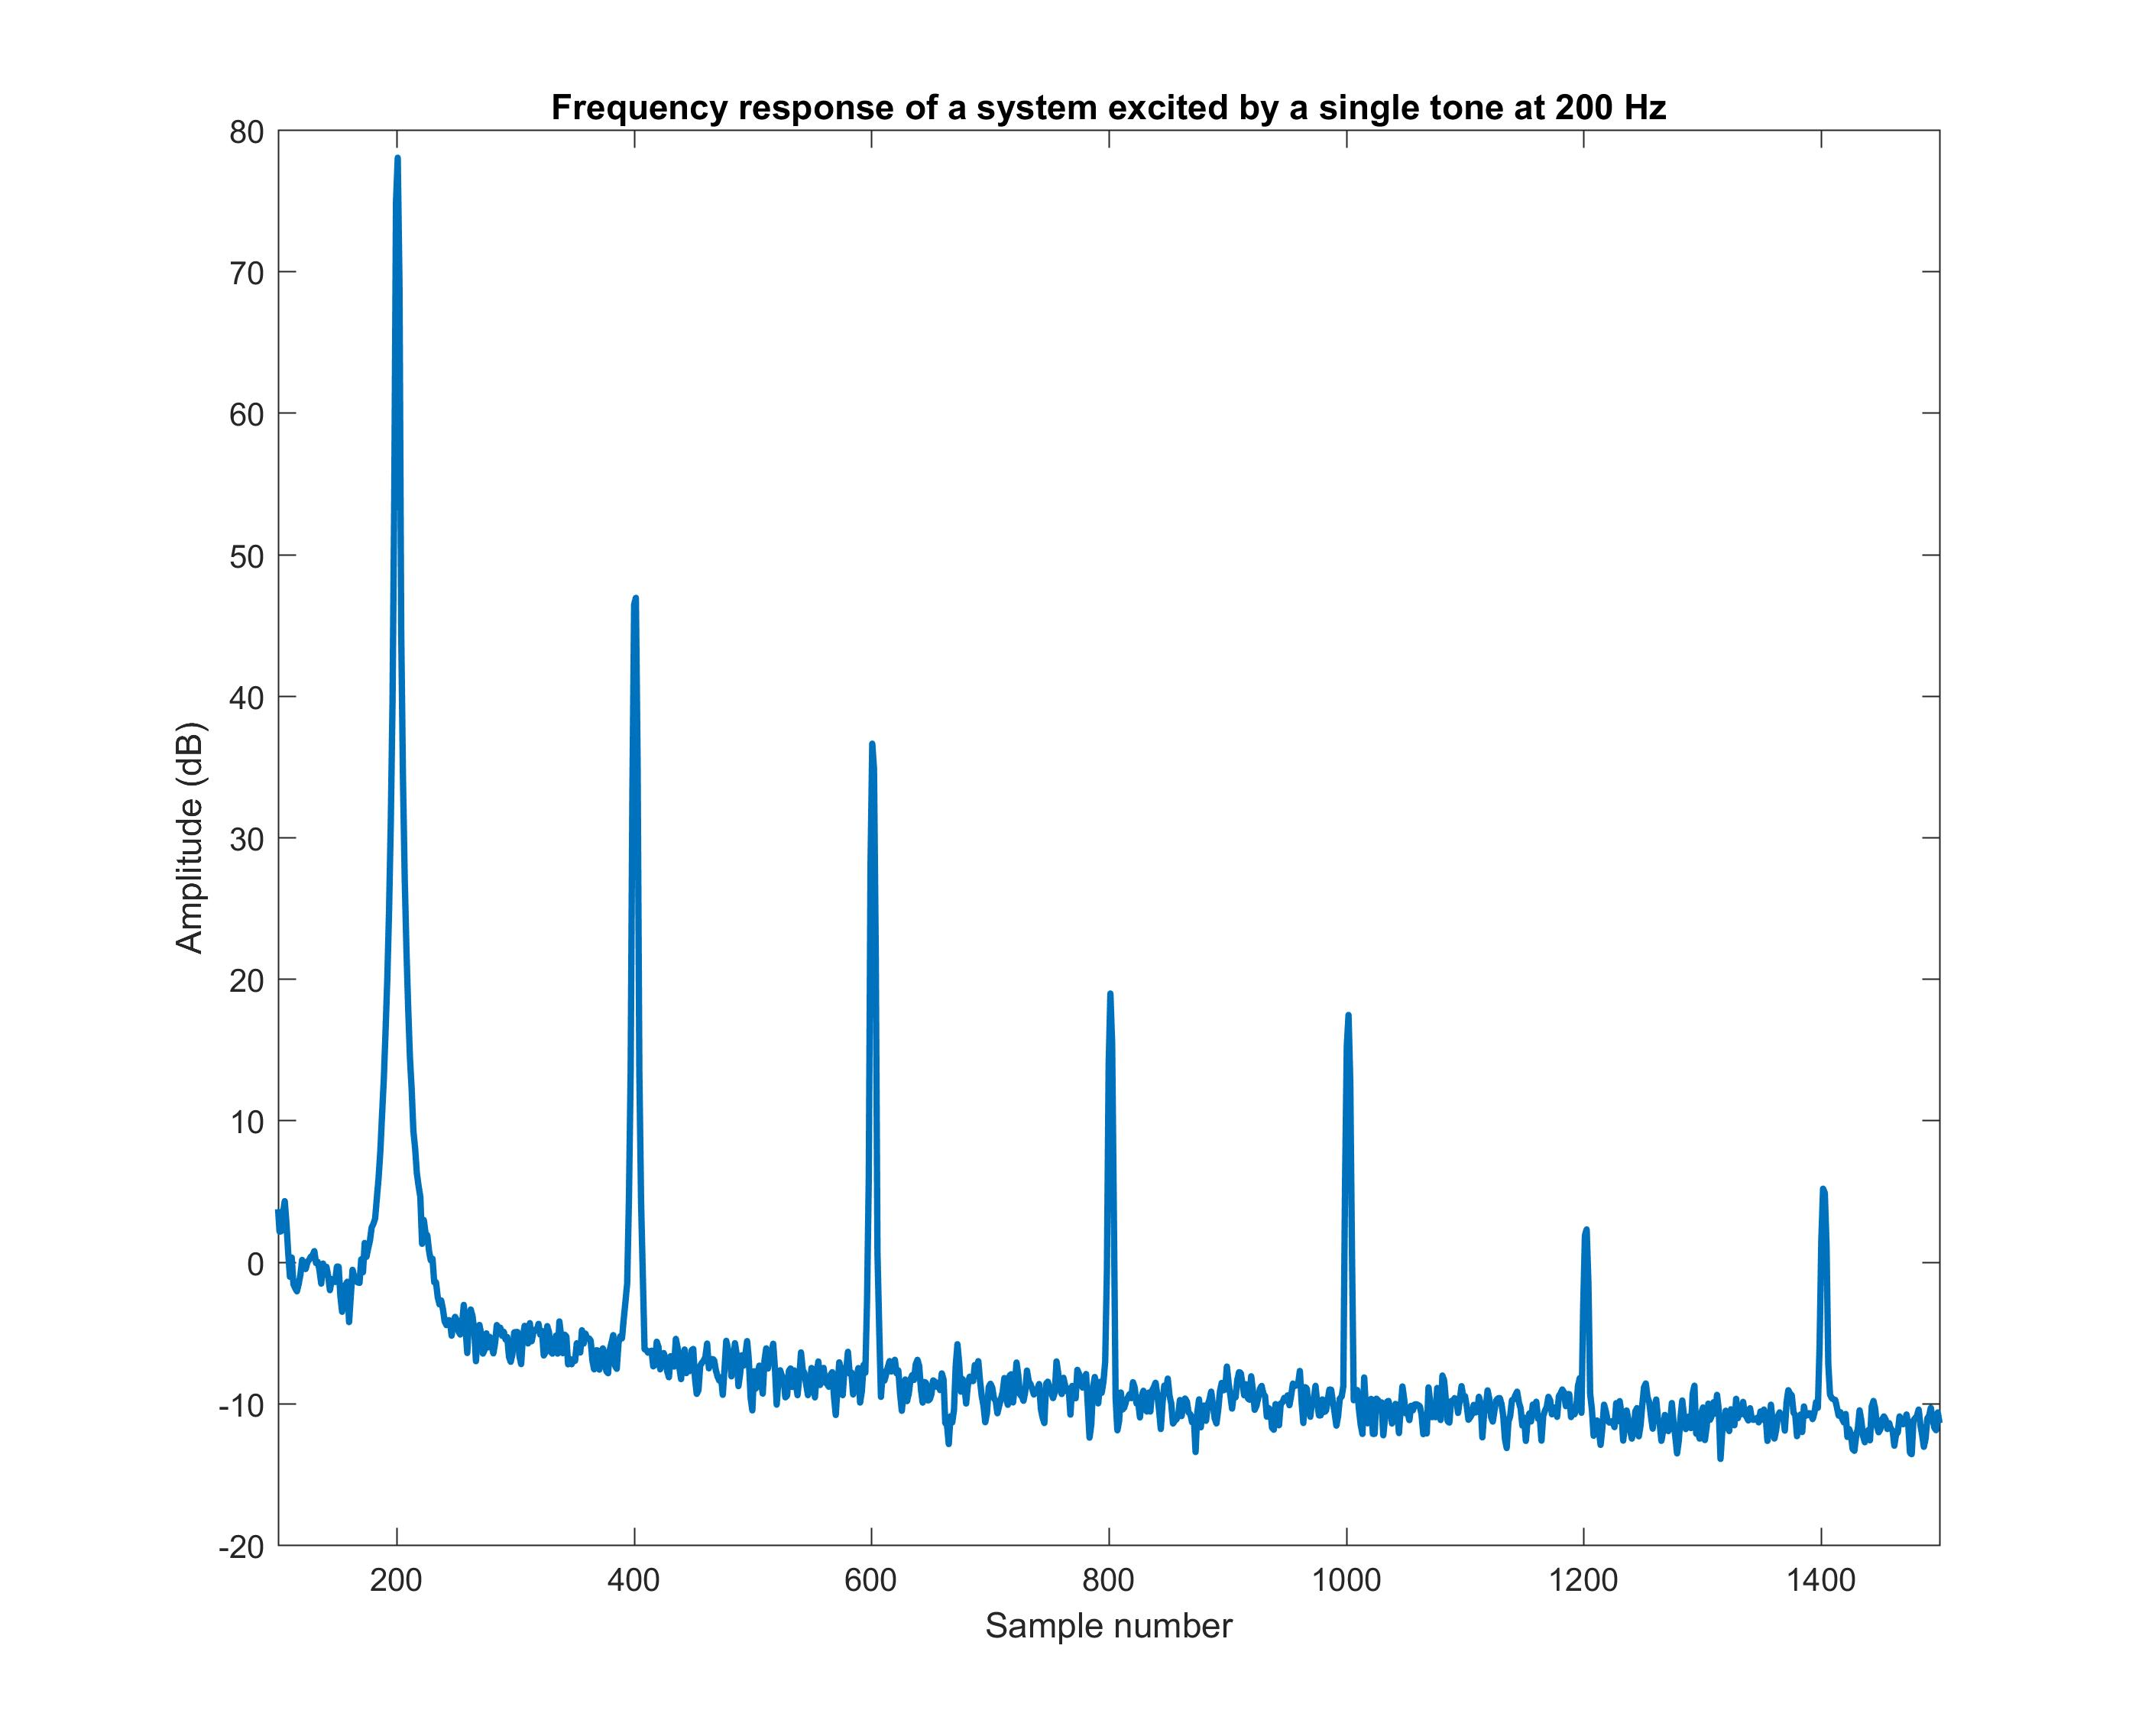
\includegraphics[width=13cm,height=13cm,keepaspectratio]{Figures/frsingletoneanechoic}
\decoRule
\caption[FR single tone]{Frequency response of the system describe in section \ref{subsec:roomsanechoic}, when excited by a $200$Hz sine-wave.}
\label{fig:frsingletone}
\end{figure}
\\
The diagram shows a peak in correspondence of the frequency of tone, plus a series of peaks, the most noticeable ones at integer multiples of the original one. As explained in section ~\ref{sec:soundgen}, this is due to speaker nonlinearities. This kind of measurements have a very high
signal to noise ratio (SNR) because all the energy of the signal is concentrated at one frequency. This, even though can give a good estimation of the (non) linearity of the system, has to be repeated for all the discrete frequencies of interest, which, for high quality sound systems range between [20-20000]Hz, or even more. A Logsweep signal energy spectrum has the convenient property of being able to occupy the whole frequency range specified and, as explained shortly after, can show the system behavior for a continuous range of frequencies.
\\
The Logsweep, also called chirp function, has the interesting property that allows to discern the linear part of the system from its higher order components by separating the impulse responses of the system for each harmonic order.
\\
The function can be mathematically expressed by

\begin{equation}
x(t) = sin \left[ 2 \pi f_1 L e^{\frac{t}{L}} \right];
\label{eqn:logsweep}
\end{equation}

where

\[ L = \frac{1}{f_1} round \left[ \frac{f_1}{ln(\frac{f_2}{f_1})} T \right]; \]
\\
$f_1$ and $f_2$ are the initial and final frequencies, $T$ is the total time of the measurements and $t$ is the instantaneous time with $0<t<T$.
\\
The wave function of a Logsweep is essentially a sine wave whose frequency increases exponentially with time. Multiples of the time of interest, $t$, show a doubling in frequency of the signal. The signal to noise ratio of the calculation is given by the time taken by the sweep, the longer the signal is, the better SNR we get.
\\
The test signal also has ramp-in and ramp-out scaling factors added to it, in order to safeguard the instrumentation. This is achieved by multiplying the first and last couple of thousands samples of the generated chirp tone by a linearly increasing set of values.
\\
A spectrogram of the Logsweep, with duration of 10 seconds, is presented below

\begin{figure}[H]
\centering
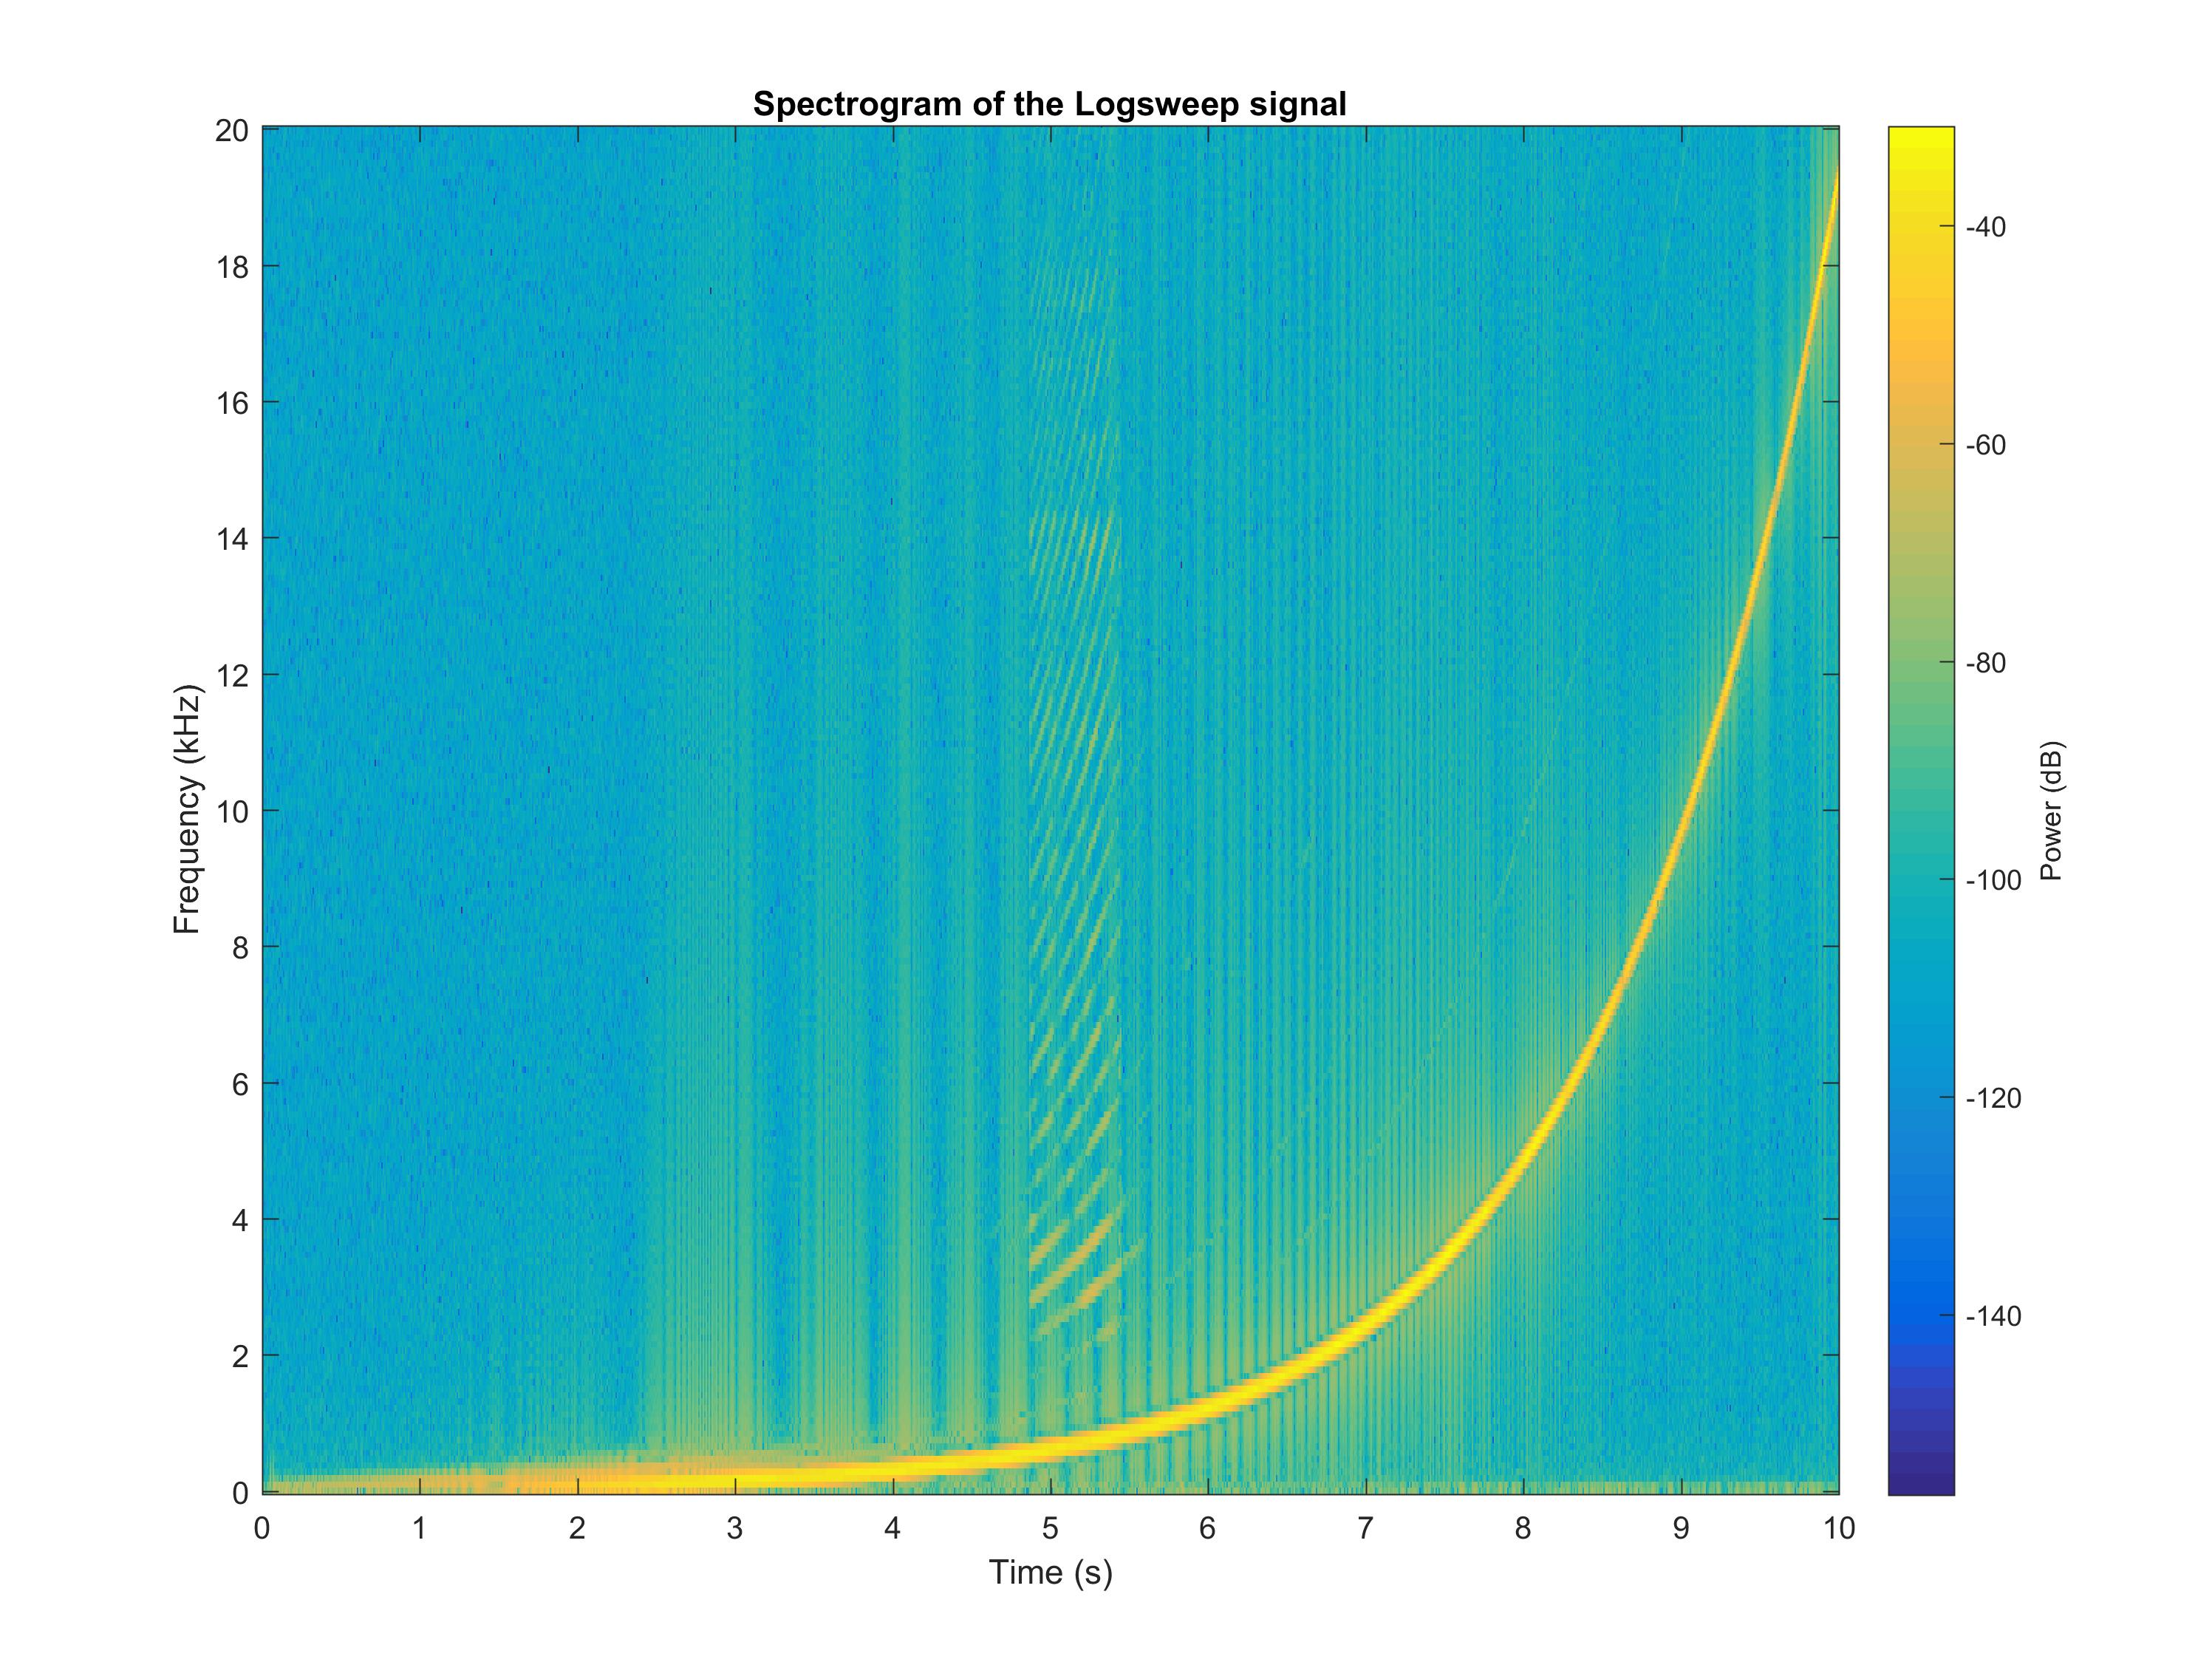
\includegraphics[width=15cm,height=16.5cm,keepaspectratio]{Figures/spectrogramlogsweep}
\decoRule
\caption[Logsweep]{The spectrogram of a Logsweep signal, with ramp-in and ramp-out of 2000 samples. The frequency scale is linear. You can also notice the higher frequencies harmonics when the signal crosses the $200$Hz mark.}
\label{fig:logsweep}
\end{figure}

Once outputted the signal and after having applied equation \ref{eqn:h}, the result is the impulse response of the system, where the harmonic components are well separated. A window filter can be applied to the resulting IR to divide each harmonic order, the frequency band of each one of those is $[nf_1, f_2]$, where $n$ is the number of higher harmonics (HH) we want to study. The graphs representing the fundamental and higher order harmonics of the system used for the tests will be presented in chapter\ref{Chapter4}.
\\
The separation between each HH is equal to $\delta t_n = L ln(n)$, this means, the more HH we want to calculate, the shorter the $\delta t_n$s are.
\\
\\
Finally, we can say that the Fourier transform of $h_n(t)$, $H_n(f)$, represented with a magnitude plot (like the one in figure \ref{fig:frsingletone}) is the most common
representation since it shows the distortion of all the harmonics as a function of the frequency.

\section{Simulated environment}
\label{sec:simenv}

The very first step for reproducing the \parencite{cai_time-domain_2014} BACC-RD algorithm was to design a simulation able to prove the effectiveness of the concept. In order to find a filter able to create some kind of acoustic contrast it was necessary to generate an appropriate impulse response for the simulated environment. The simulation room was composed of 8 ideal sound sources, each one $10$cm apart one another and 32 ideal impulse response detection points, divided in two zones. Each point is $5$cm apart from its neighboring ones. The distance between the simulated sound source and the closest simulated detection point, with respect of the x axis, is $3$m. The simulated room is represented in figure \ref{fig:simroom}.

\begin{figure}[H]
\centering
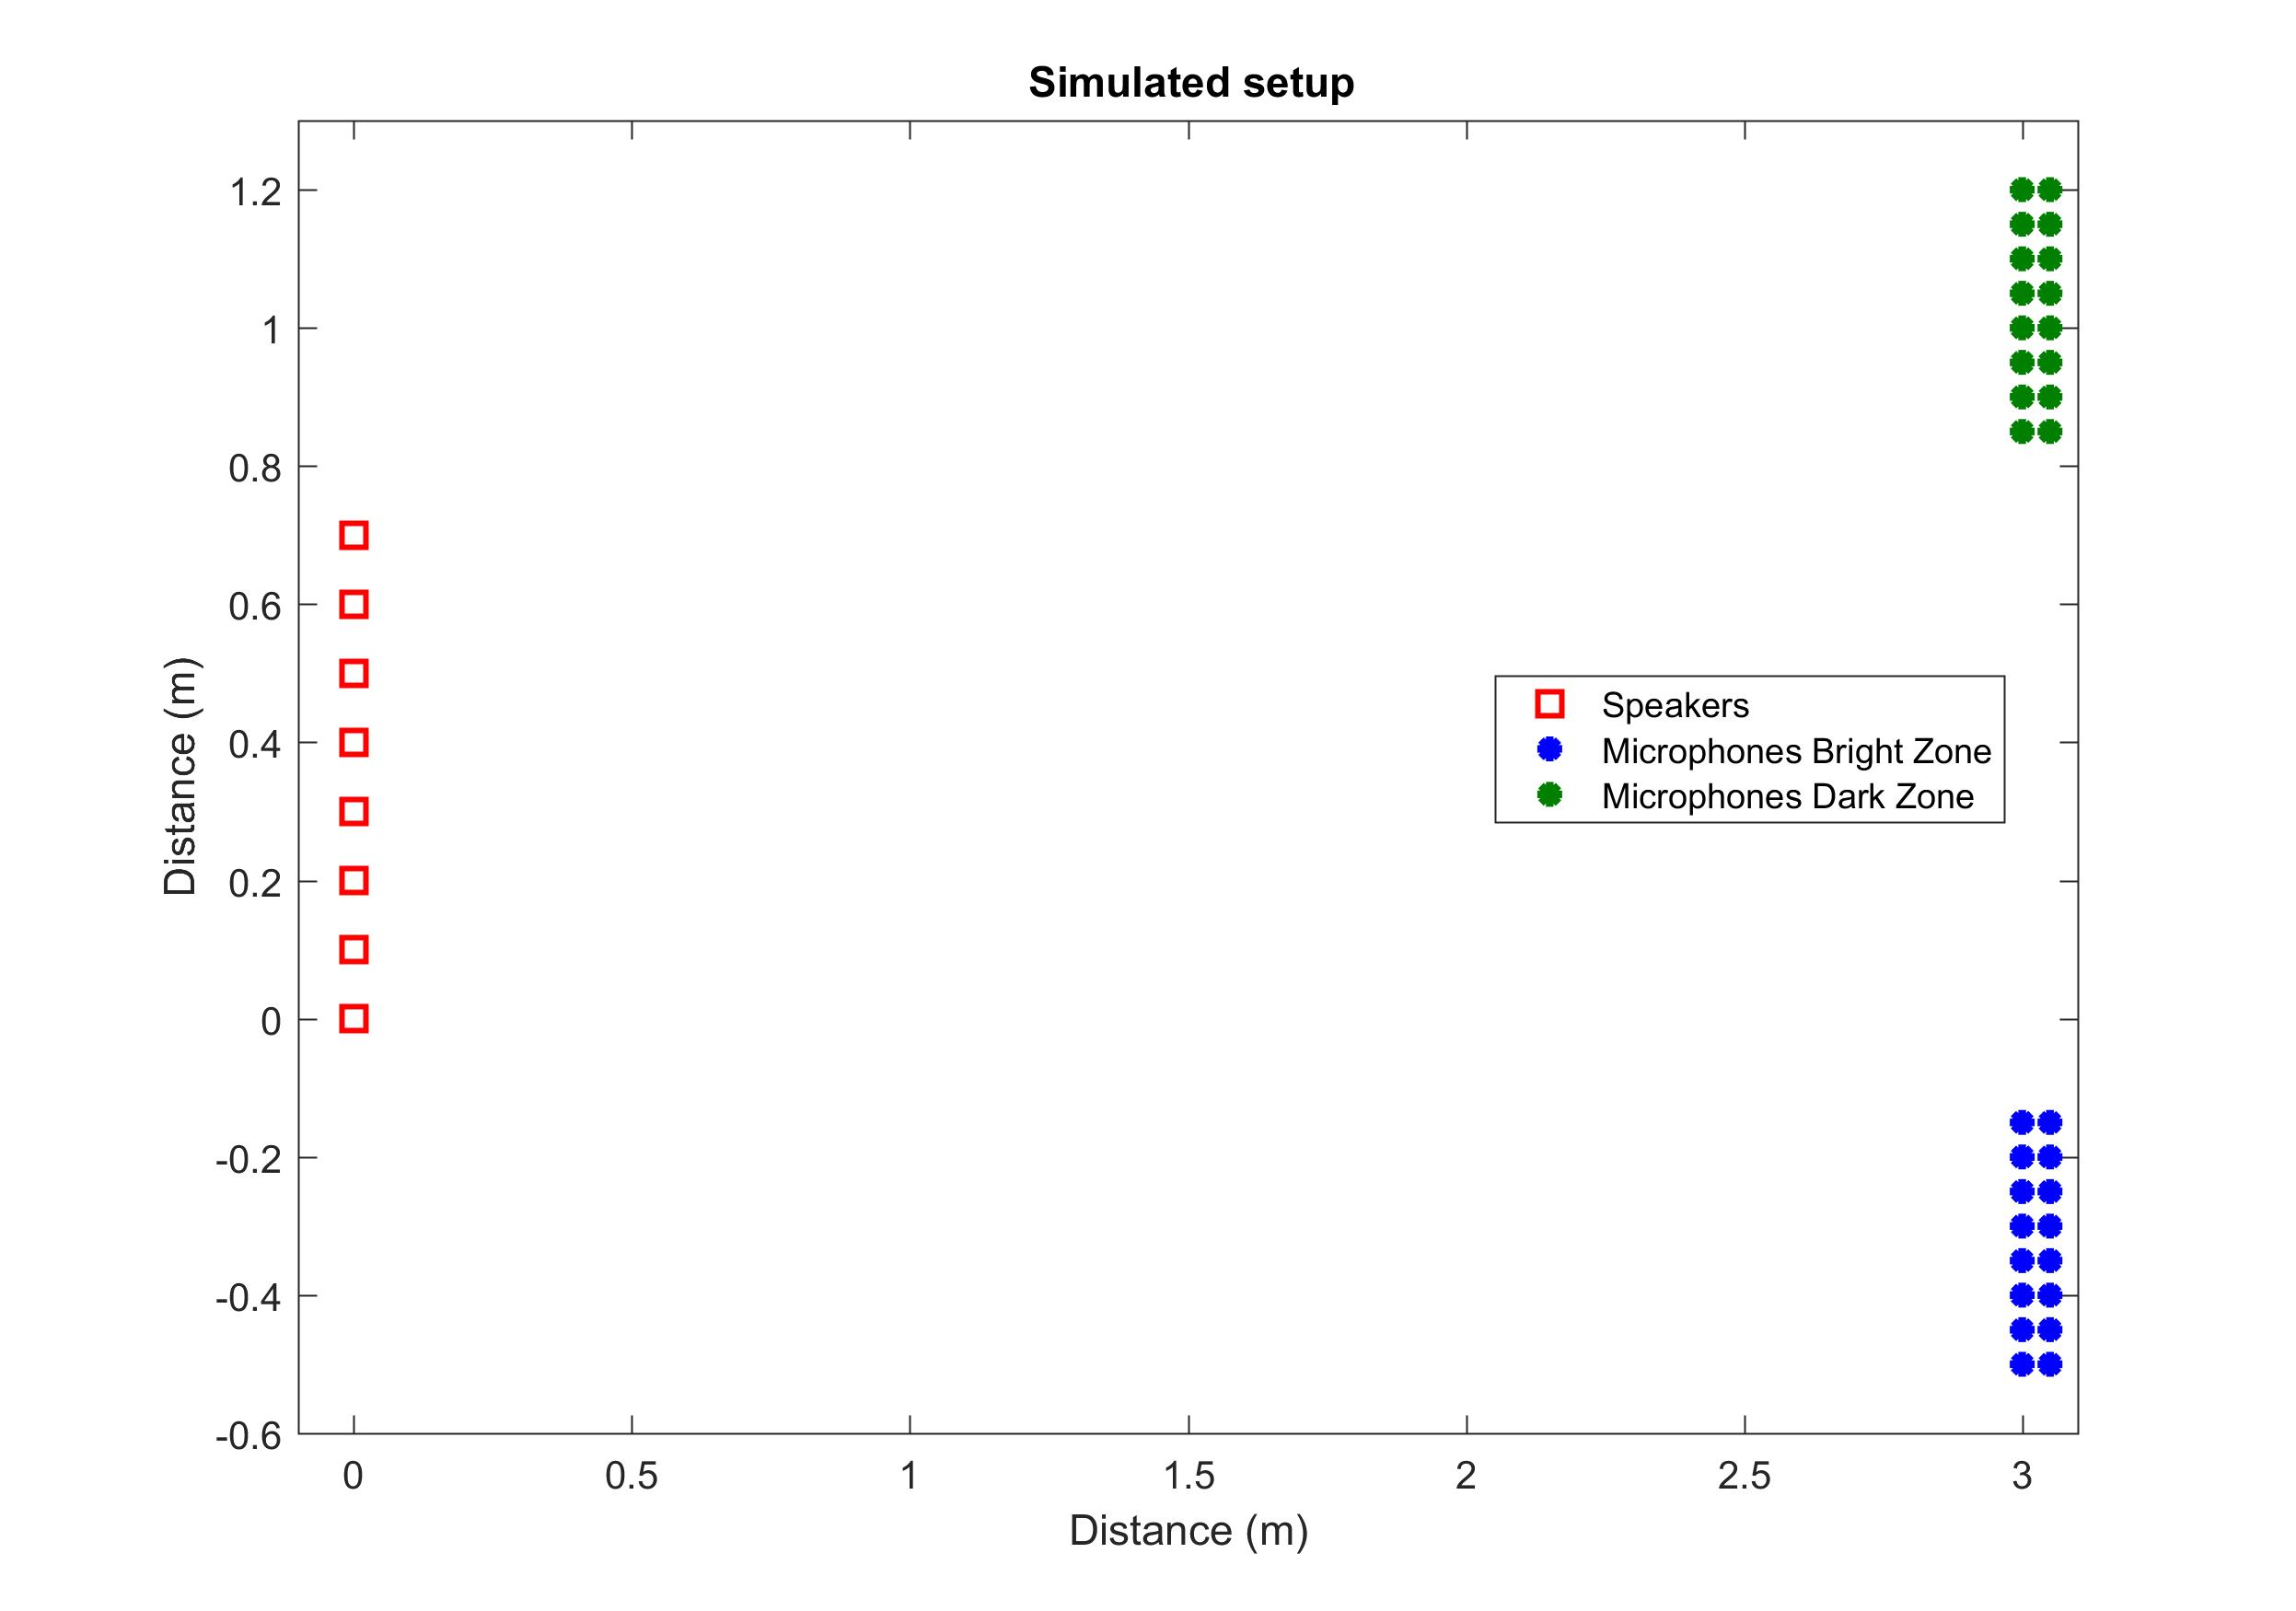
\includegraphics[width=14cm,height=14cm,keepaspectratio]{Figures/simroom}
\decoRule
\caption[Simulated room]{Simulated room. The red stars represent the speaker and the green and blue ones represent the microphones in the two zones.}
\label{fig:simroom}
\end{figure}

As shown in the figure above, the two clusters of detection points are referred to as bright and dark zone, this is because we want to design a filter that is able to limit the total acoustic energy in the area delimited by the green points, while leaving the other zone as unaltered as possible.
\\
Thanks to the Green's function it was possible to design a simulated impulse response of the system. A random signal is supposed to be outputted by each of the red source points (sequentially) and detected by all of the control points in both zones. The propagation of the wave has been calculated using equation \ref{eqn:green}. The intensity and the sample number of the spike that appears on the IR depends on the relative distance between source and detection points and the sampling frequency. This is because the Green's function is expressed also as a function of the distance. The impulse response of the system, as detected in the lower-left point in the bright zone of coordinates (3,-0.5) and emitted by the source of coordinates (0,0) is shown in Figure \ref{fig:simir}. Of course, since the impulse response is in the time domain, the result elaborated by the Green's function has been inverse Fourier Transformed.

\begin{figure}[H]
\centering
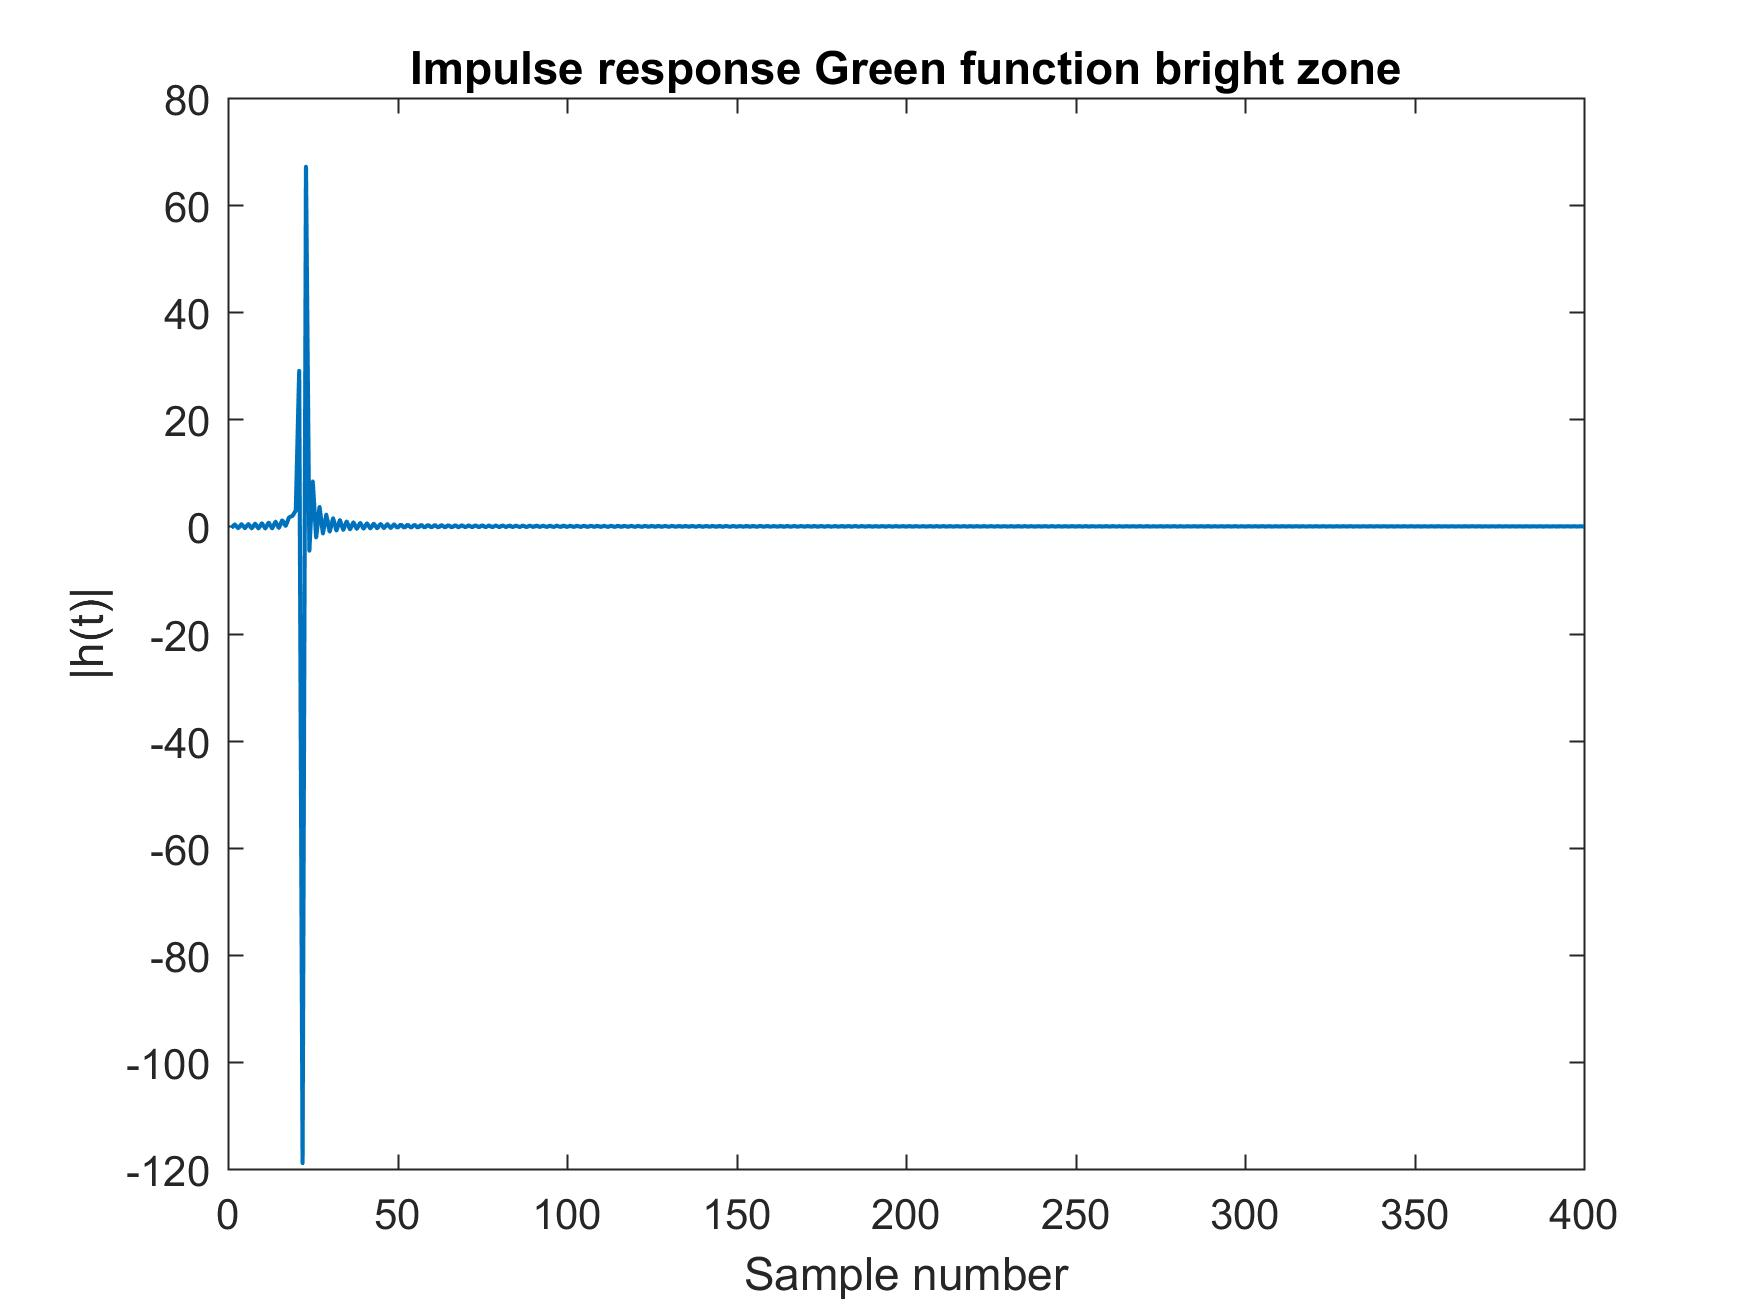
\includegraphics[width=15cm,height=15cm,keepaspectratio]{Figures/simir}
\decoRule
\caption[Simulated IR]{Simulated impulse response of the system using the Green's function.}
\label{fig:simir}
\end{figure}

If we were to replicate the same configuration in figure \ref{fig:simroom} of speakers and sound zones in any real environment, even the anechoic chamber, and apply the BACC-RD algorithm to generate some acoustic contrast, we would have had a lower result with respected of the one obtained in the simulation. This is ascribable to the fact that the power amplifiers and A/D converters add noise (either in the analog or digital domain, noise can be expressed in terms of bit error rate in the latter), the inherent noise in the microphones and the reflections present in the room, which, of course, cannot be \textit{completely} anechoic, especially when dealing with wideband signals, the kind used in all the ACC scenarios evaluated.
\\
This parting from the simulation shouldn't surprise the reader, since it is the price one has to pay when having to deal with real equipment. Still, the simulated environment has to be considered a development tool for the algorithm itself, we will prove that we are able to achieve acoustic contrast using the hardware described later in this chapter.
\\
\section{The test rooms}
\label{sec:rooms}

The simulated environment, generated using MATLAB, proved fundamental for debugging and checking the validity of the code implementing the BACC-RD algorithm. But, for the reasons already explained in \ref{sec:soundgen}, a simulation using the Green's function is insufficient to analyze the performance of the algorithm in a real environment. In the section below the reader will find a description of the rooms used for running the tests.

\subsection{Anechoic chamber}{}
\label{subsec:roomsanechoic}

The room used for most of the tests was the anechoic chamber in the AUDIOLAB facilites of the Aarhus University. The reader should assume that all the test were conducted in the chamber, unless otherwise specified. The chamber is a test room rated for sound experiments. Both the floor, the walls and the ceiling are acoustically dampened by acoustic foam. The foam in most of the surfaces has a length of $85$cm This means that its effectiveness in dampening the sound is limited to waves roughly shorter than $\frac{1}{4} \lambda = 3.40$m, or \tld$100$Hz.

\begin{figure}[H]
\centering
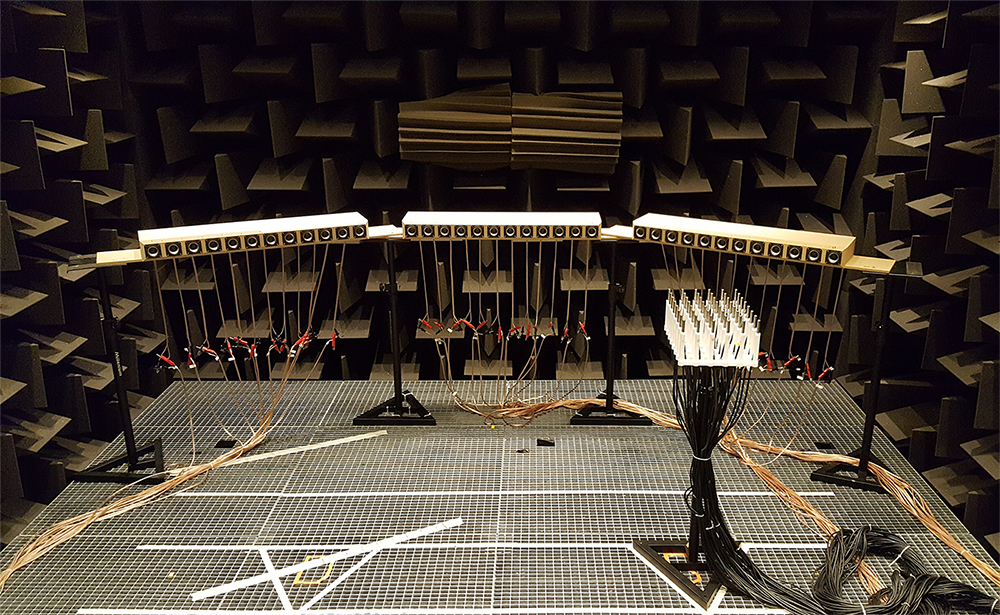
\includegraphics[width=14cm,height=15cm,keepaspectratio]{Figures/anechoic}
\decoRule
\caption[Anechoic chamber]{The anechoic chamber in the AUDIOLAB facility of the Aarhus University.}
\label{fig:anechoic}
\end{figure}

The chamber dimensions are $6\text{x}5\text{x}4.5$m (length, width, height). The walkable area is made by a metal grid, standing $1.20$m above the actual floor level. The grid is mechanically dampened from the rest of the room. The equipment is secured on the pavement with plastic straps in order to reduce vibrations.
\\
The background noise of the room is \tld$17$dB, this was measured by making a $10$ seconds recording of the room (without playing any sound).

\subsection{Listening room}{}

The second test environment was the listening room of the AUDIOLAB facility in the Aarhus University. It is a room designed to simulate a real living room environment, with chairs, tables and bookshelves. The furniture provides a multitude of reflective surfaces that spread the sound, meaning that the reverberation time is understandably higher than the one in the anechoic chamber. This room has been used to demonstrate the feasibility of the study in an every day scenario.
The room dimensions are $4.75\text{x}4.75\text{x}2.70$m (length, width, height).

\begin{figure}[H]
\centering
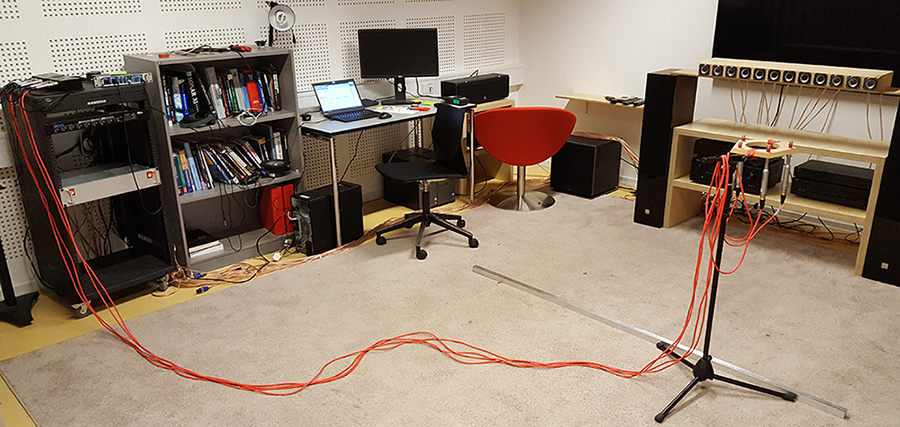
\includegraphics[width=14.5cm,height=15cm,keepaspectratio]{Figures/listeningv2}
\decoRule
\caption[Listening chamber]{The listening room of the AUDIOLAB facility.}
\label{fig:listening}
\end{figure}

The background noise in this room is \tld$25$dB. This value is measured when the instruments (especially the power amplifiers, which have active cooling) inside the room were turned on.

\section{Hardware}
\label{sec:hw}

This sections provides some details regarding the hardware that allows the change of domain of the signal, specifically from the digital domain of the data coming from the PC running MATLAB to the analog domain used by the loudspeaker, to the mechanical domain of the sound recorded by the microphones, only to be converted back to an analog and then digital signal returned to the PC.

\subsection{A/D converters}{}

The conversion from and to the PC running the MATLAB code was performed by some A/D and D/A converters. The ones used for the anechoic chamber are respectively an RME M-32 AD and an RME M-32 DA. Each one of them is equipped with 32-channels. Since the total numbers of speakers in the chamber is $36$ and the microphones in the matrix are $48$, two unit of each converter are used. These pieces of hardware are daisy chained through an optical connection that provides an useful single interface to communicate with the PC. Thanks to Playrec it was enough to specify the target device (a digital interface) and the firmware of the converters themselves took care of synchronization and delivery of the signals between the units.
\\
the D/A converters are connected to two ICEpower1000ASP power amplifiers. These unit are the ones directly connected to the loudspeakers in the anechoic chamber. A gain attenuator of $-20$dB is used in each line after the amplification, to prevent damage to the loudspeakers.
\\
The A/D converter are connected to the custom microphone power amplifiers (inside the chamber) that power up the Panasonic microphones (the ones in figure \ref{fig:anechoic}).
An additional line of the A/D is reserved for an Nti microphone (described in section \ref{subsec:mics}), which requires its own phantom power, positioned in the signal chain between the two, specifically, the power unit used is a Millennium PP2B.
\\
One data line is directly connected from the D/A to the A/D converter. This lines bypasses the loudspeakers and microphones completely. Feeding data trough this channel reveals how long of a delay having this equipment introduces into the signal chain. It is also a useful monitor that allows us to see if the input signal, intended to the loudspeakers is correct.
\\
\\
The listening room is provided with some more portable hardware, namely the RME Fireface UC, which acts as A/D and D/A converter. The Fireface output lines are connected to a single ICEpower amplifier, which drives the loudspeakers. A gain attenuator of $-20$dB is used again. The microphones are powered by two other Millennium PP2B units, which have 2 I/O lines each, similarly as the one used in the anechoic chamber.

All the converters allow for two different sampling frequencies, $48$kHz or $96$kHz, the one that will always used will be the former.

\subsection{Loudspeakers}{}
\label{subsec:speakers}

The choice of the best set of loudspeakers among the available ones has been the first development steps of this project. Checking the inventory of the laboratory, two were the models deemed suitable. The SB acoustics SB65WBAC25-4 $2.5$ inches and the AuraSound NS2-326-8AT $2$ inches speakers.
\\
The first one has an impedance of $4$Ohm and a power capacity of $20$W RMS. The second has an higher impedance of $8$Ohm, but can output a maximum of $15$W RMS.

\begin{figure}[H]
\centering
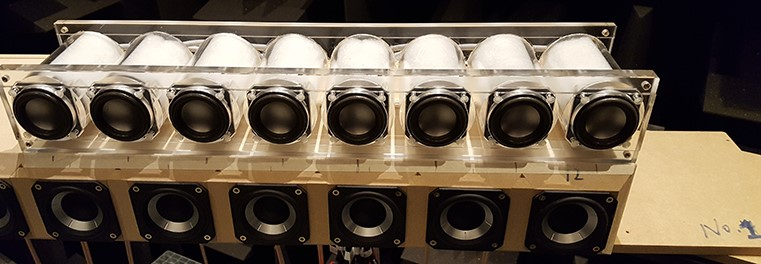
\includegraphics[width=10cm,height=10cm,keepaspectratio]{Figures/aurasb1}
\decoRule
\caption[Aura speakers]{Aura speakers array on top of the SB array on the left side of the anechoic chamber.}
\label{fig:aurasbspeakers}
\end{figure}

The frequency response of the two models is presented below. The speaker used for this measurement are the ones in the figure above, all 8 speakers of the Aura unit (on top) and the 6 rightmost speakers of the first for the SB array (the array on the left in figure \ref{fig:anechoic}). The SPL level has been measured five times and the results averaged, using the same identical input signal (a Logsweep signal lasting for 10 seconds), the results show an SPL of $98.0$dB $\pm0.2$dB for the Aura and $97.1$dB $\pm0.3$dB for the SB arrays. The microphone used was the Nti model at a distance of $1$m.

\begin{figure}[H]
\centering
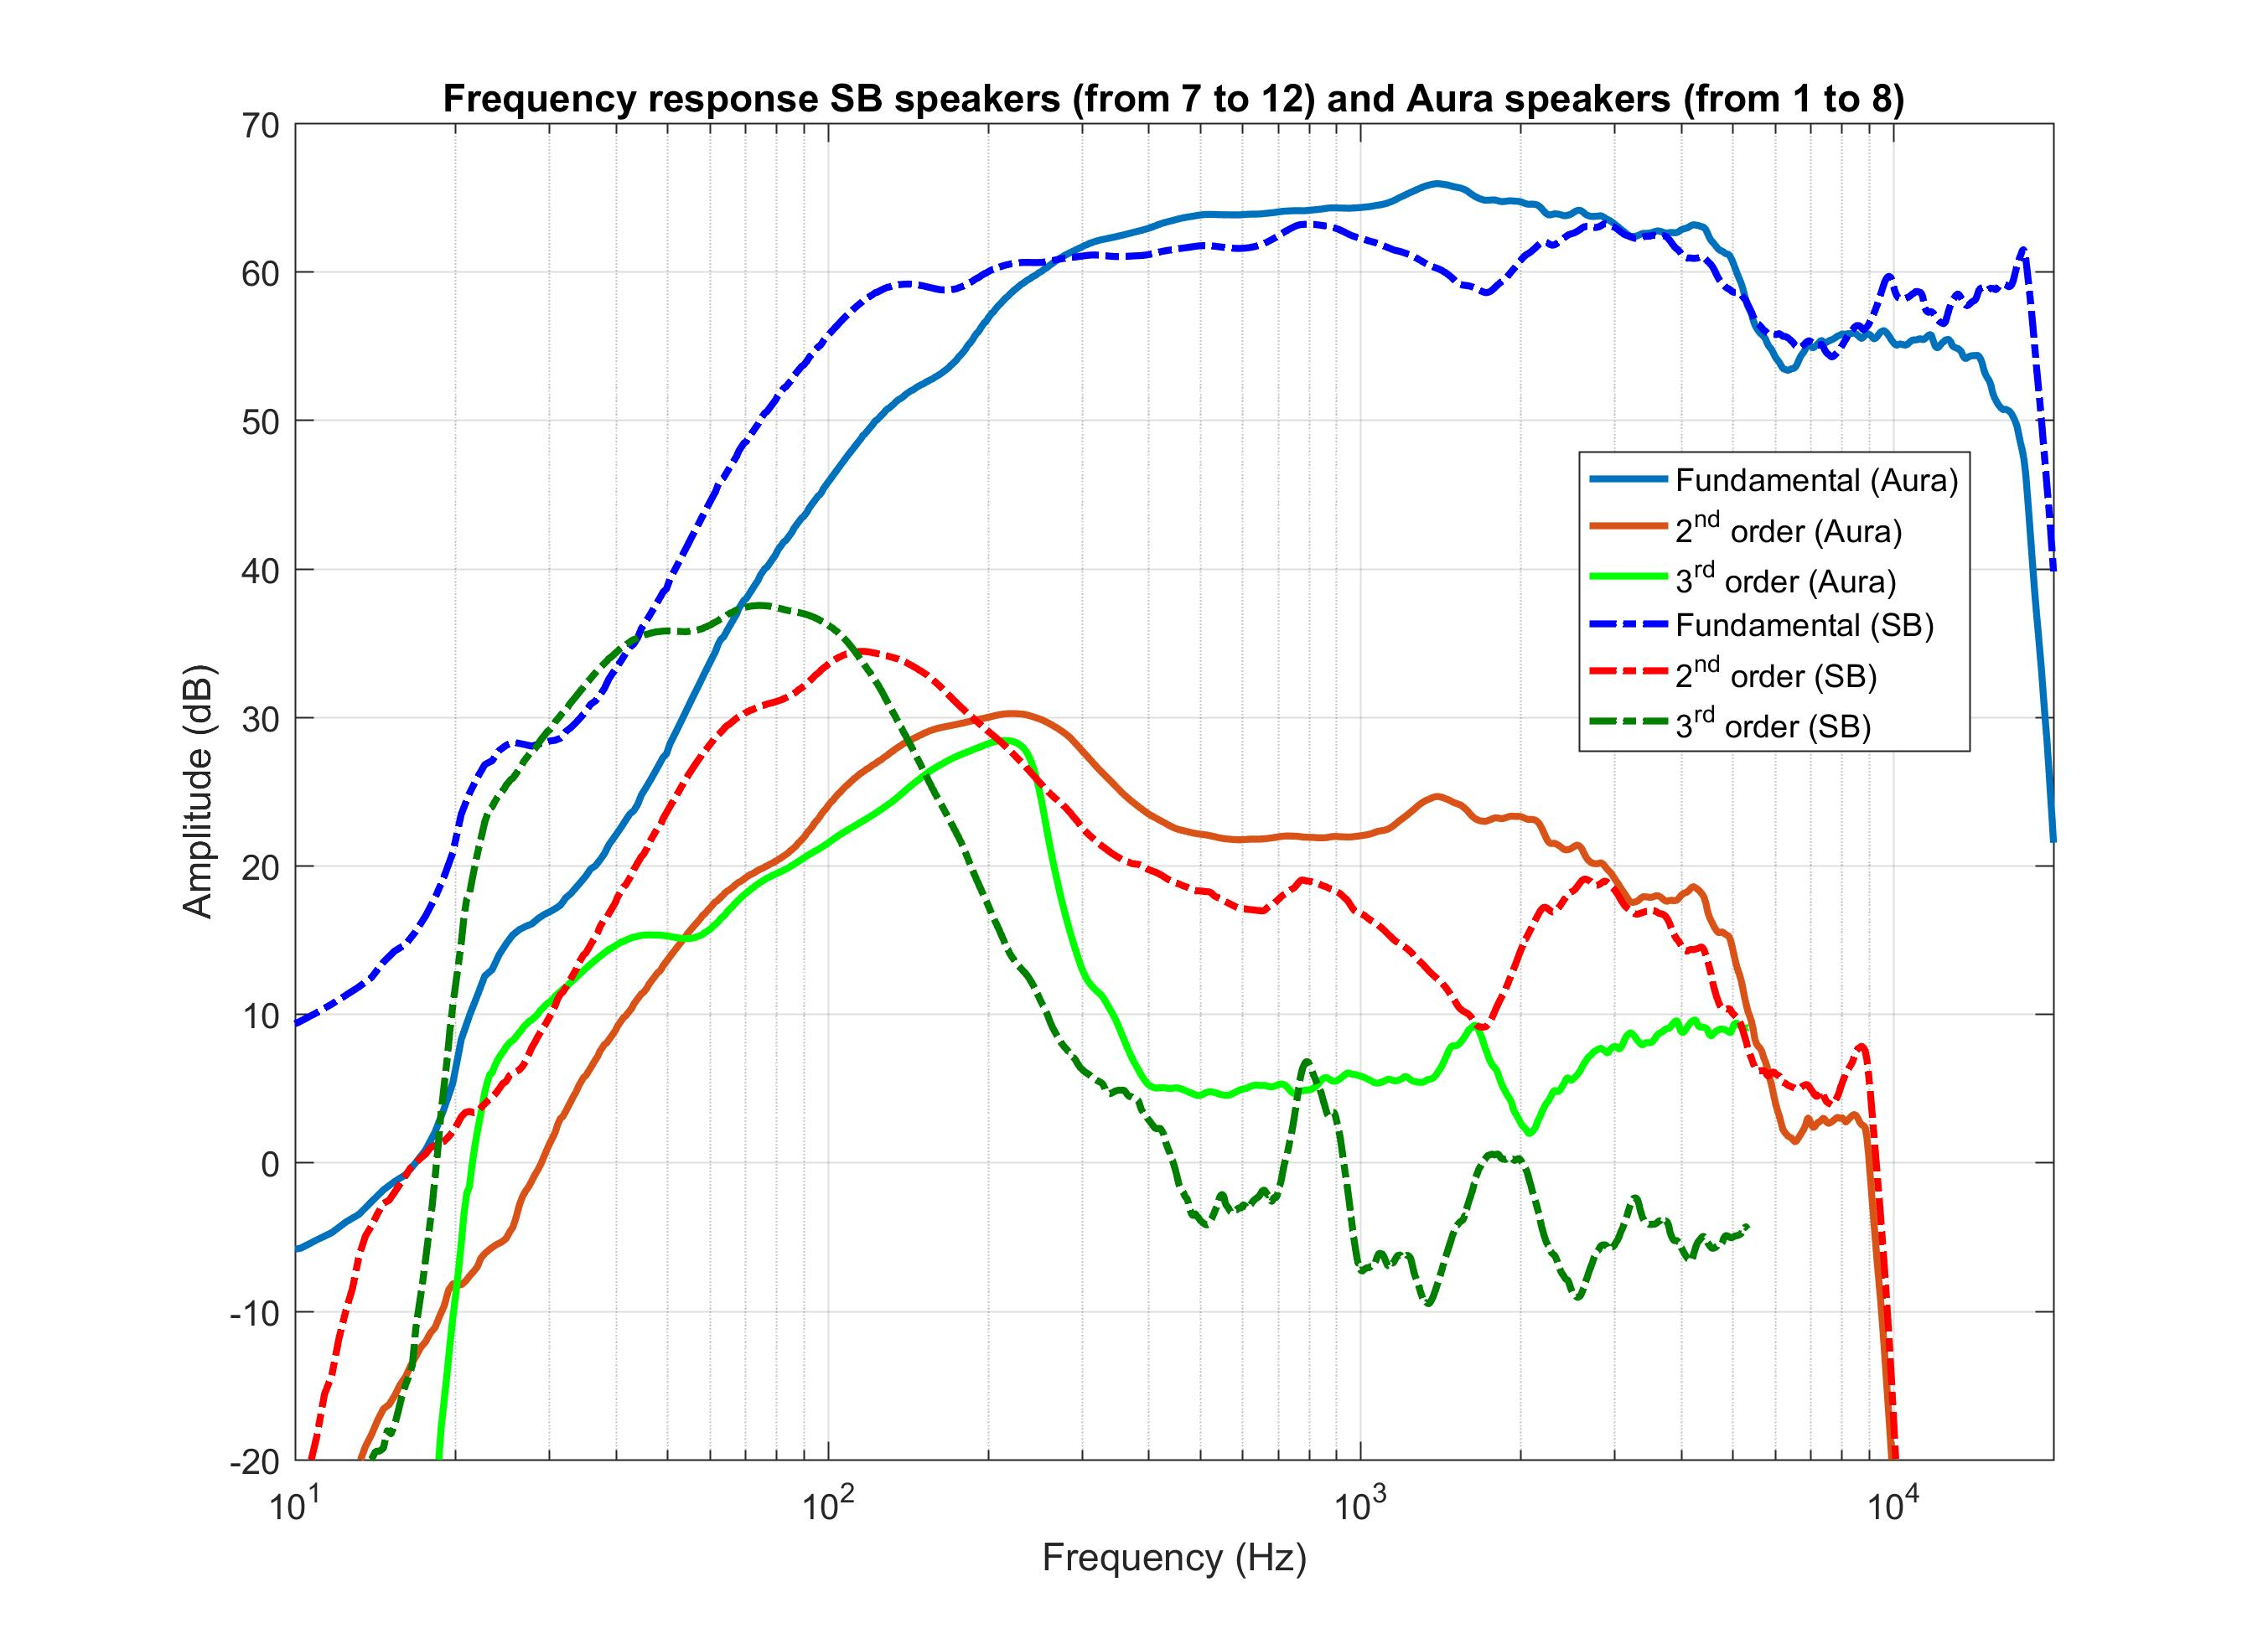
\includegraphics[width=15cm,height=15cm,keepaspectratio]{Figures/aurasbfreq}
\decoRule
\caption[Anechoic chamber]{Comparison between the frequency response of the SB speakers (dotted line) and Aura speakers (solid line). The first 3 harmonics are represented here.}
\label{fig:aurasbfreq}
\end{figure}

In section \ref{sec:soundgen} we explained how the amplitude is an important parameter when it comes to determine the amount of distortion generated by speakers playing a sound. Since the two models have different characteristics, we need to make sure to use a sound level that is comparable. This is done by scaling the amplitude of the input signal $-1\le x\le 1$ using the formula
\[x=\text{input signal}^{(\text{output level in relative scale}/20)}\]

This means that we are going to use a relative scale, which is a pure number, to represent the output level. The maximum value allowed in this scale is $0$, any value beyond this point will be translated by the amplifiers in a value that will end up damaging the speakers.
\\
We can then convert this relative scale to a value in decibels by dividing the root mean square value of the recorded Logsweep signal to the reference sound pressure level (SPL), which is $2\textbf{x}10^{-5}$Pa. Expressed in mathematical notation it can be written as
\[\text{SPL in dB}= 20 \log_{10} \left[\text{rms}(x)/ \text{reference SPL} \right]\]
\\
In the following table we present the conversion between the SPL and the relative scale for the loudspeakers belonging to the central array of SB units, the driver playing were from 15 to 22. The reason why this results presented are for those specific driver units is because, as we will later explain, those were the exact units chosen to carry out most of the experiments of chapter \ref{Chapter4}, hence the following table will be an useful tool to convert the relative scale to a dB value. The conversion only has meaning in the anechoic conditions, changing environment (using, for instance, the listening room) or position of the microphones means we have to re-calculate the correspondence between relative scale and the corresponding SPL, the usefulness of this conversion is given by the fact that the many experiments in the anechoic chamber will almost never see the position of the microphones change (except in those rare case when it will be specified). The recorded SPL level is made by averaging the recordings of the Panasonic microphones (described in the next section) $20, 21, 28, 29$ (the four innermost in the microphone matrix in figure \ref{fig:mics}) situated in the bright zone, $1.40$m from the center of the speakers. This experiment was repeated five times. The margin of error of the measurement was $\pm 0.3$dB.

\begin{table}[H]
\label{tab:relativescale}
\centering
\begin{tabular}{ll}
\toprule
Relative scale & SPL (dB)\\
\midrule
-40            & 69.60\\
-35            & 74.60\\
-30            & 79.70\\
-25            & 84.50\\
-20            & 89.50\\
-15            & 94.10\\
-10            & 98.20\\
\bottomrule\\
\end{tabular}
\caption{Comparison between output level and corresponding SPL.}
\label{tab:relativescale}
\end{table}

If we graph the two scales together we can see that the amplification is pretty much linear, which is to be expected when applying different gains to the input signal.

\begin{figure}[H]
\centering
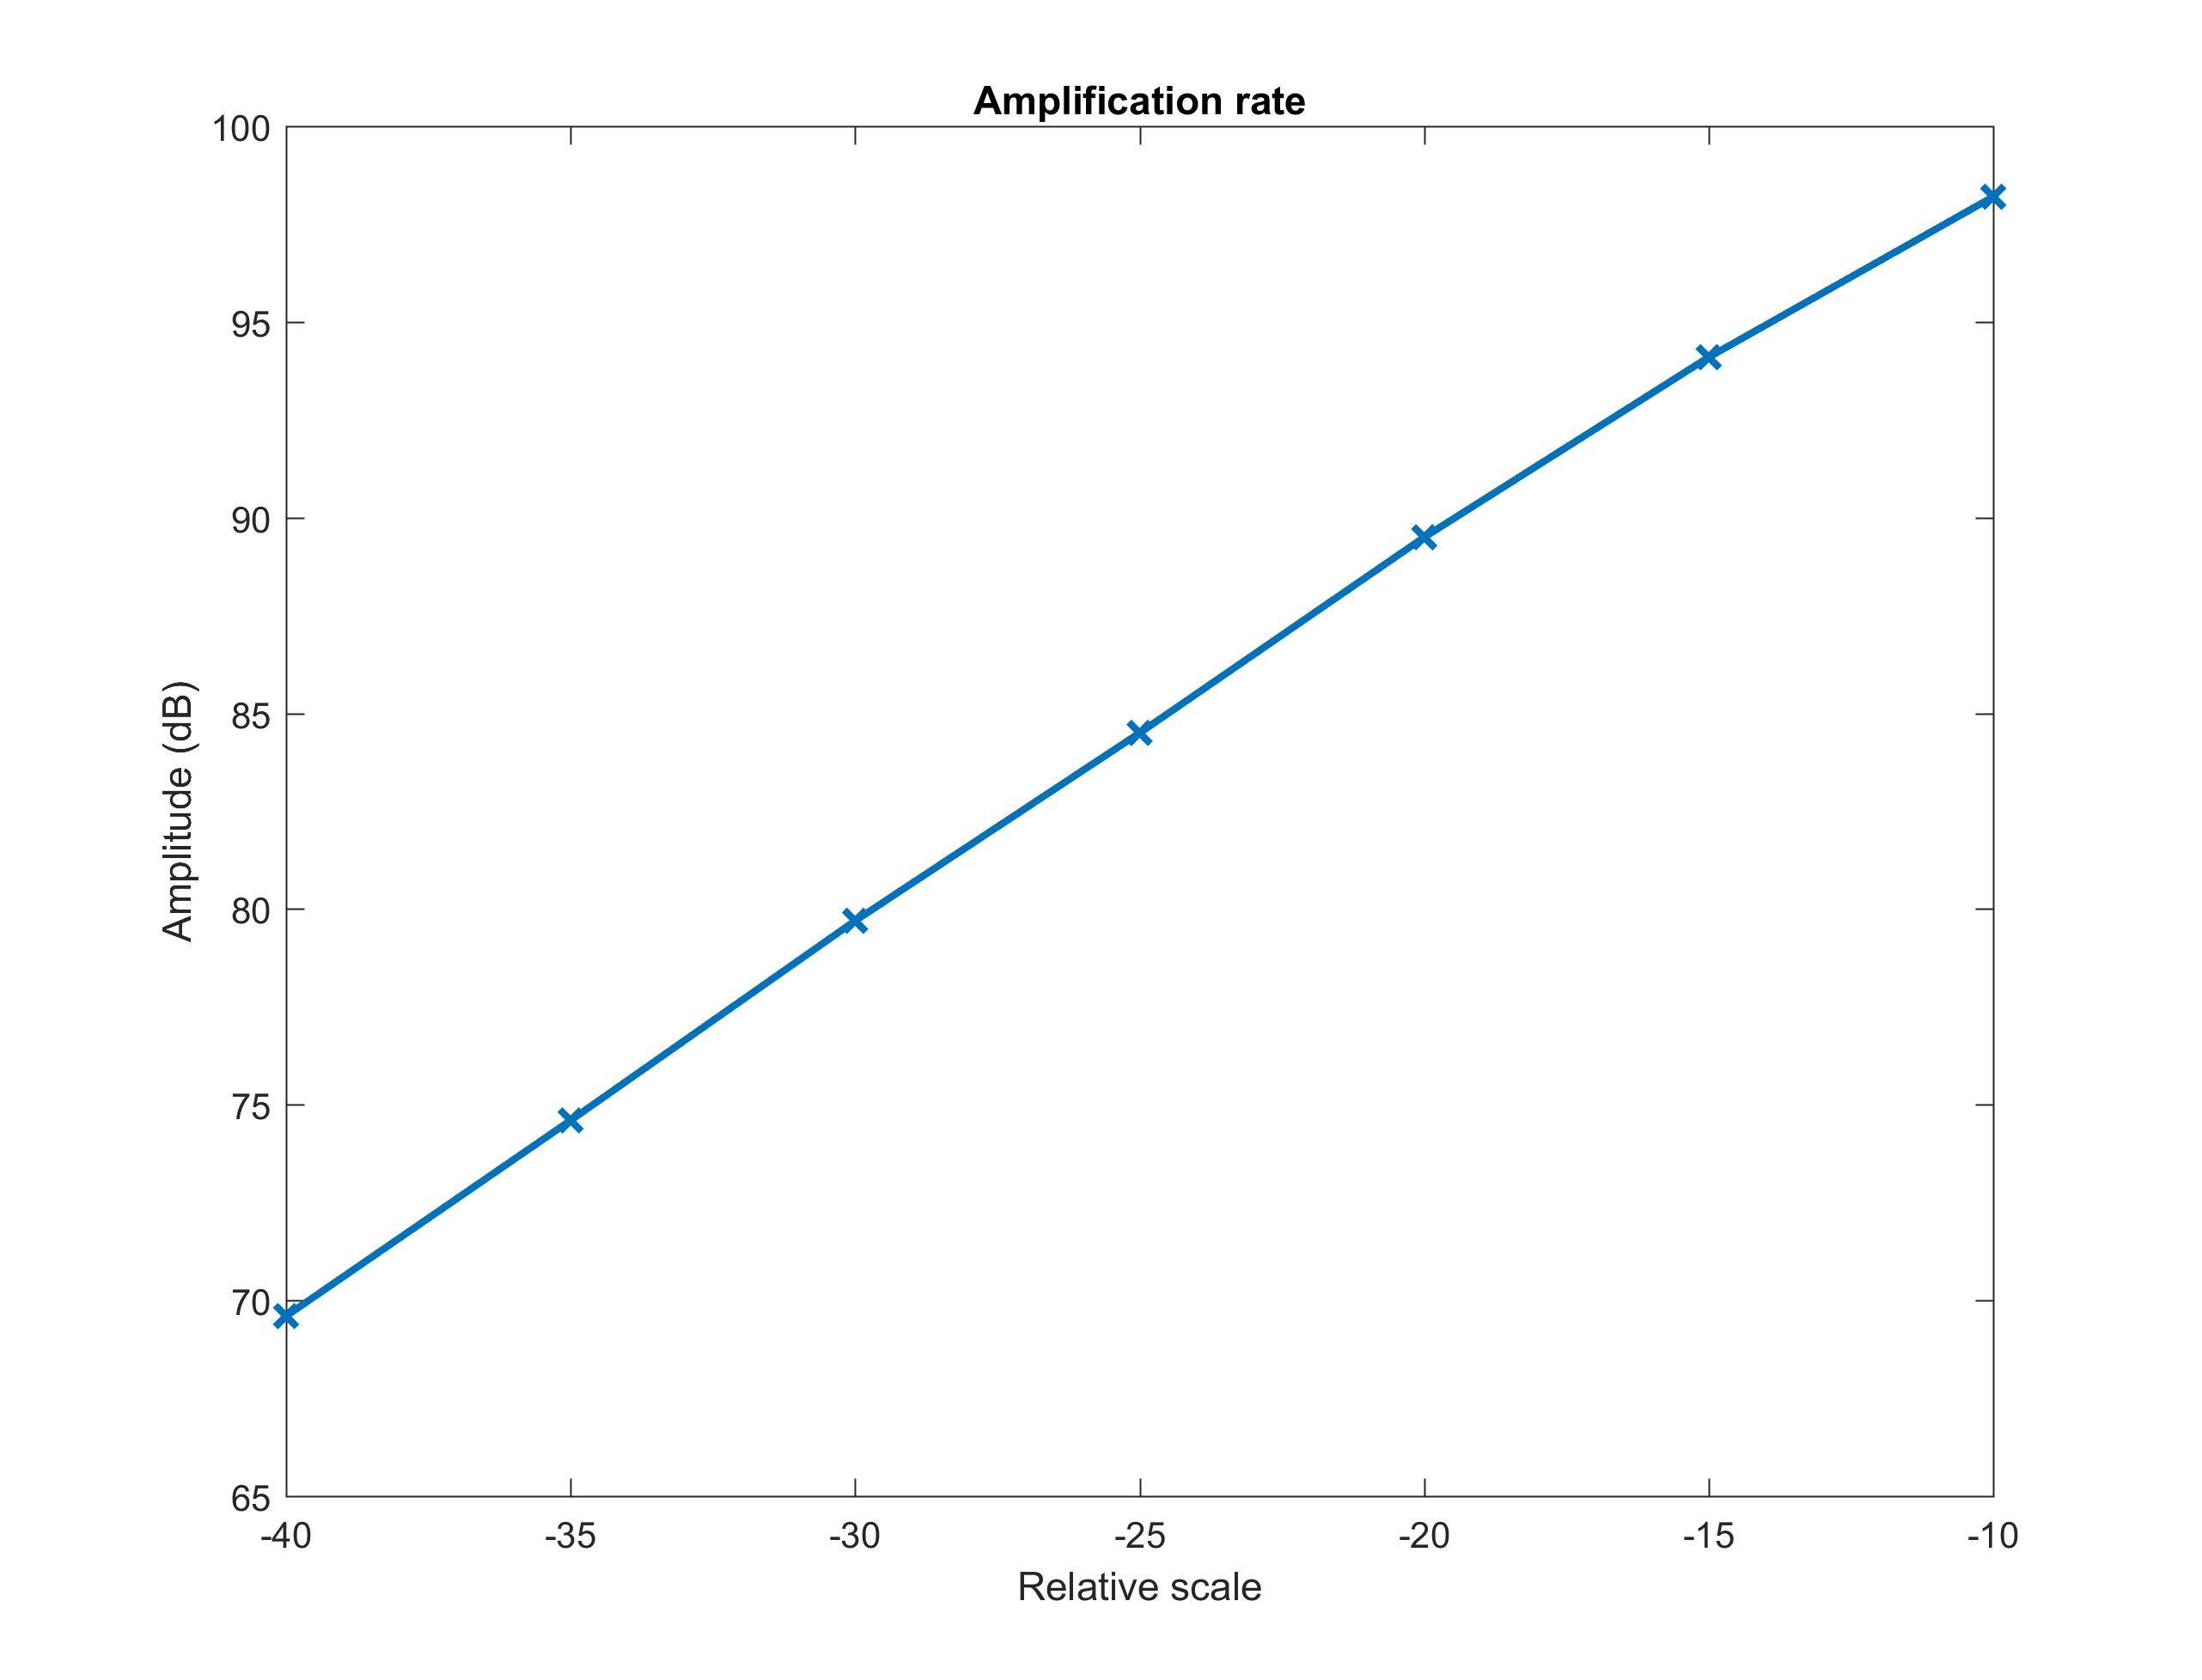
\includegraphics[width=13.5cm,height=13.5cm,keepaspectratio]{Figures/amplification}
\decoRule
\caption[Amplification factors]{Comparison between the relative scale and the corresponding SPL values.}
\label{fig:mics}
\end{figure}

All the results obtained using this set of loudspeakers will be represented using the relative scale above. When this is not the case the SPL level is specified together with position and model of the microphones used.
\\
The comparative study of the two models and the reasoning for the choosing of the SB speakers is described in section ~\ref{subsec:sbchoosing}.
\\
\\
Finally we have to measure the free field attenuation in the room, this is the value (in dB) that indicates how much the sound pressure decreases depending on the distance. This is the absolute lower minimum that we wish to increase with the ACC algorithm. By playing loudspeaker 22 (the rightmost of the one used in the center array in the anechoic chamber) we can measure an attenuation of \tld$2dB$ between the SPL measured in the bright zone versus the one measured in the dark zone. 

\subsection{Microphones}{}
\label{subsec:mics}

The microphones used for the experiments are of three kinds. The first and most used, situated inside the anechoic chamber are the Panasonic WM-61A, omnidirectional, condenser type microphones. They are pad-type circular instruments with a diameter of 0.6 cm. They draw their 2V at 500$\mu A$ of power from two custom made power supply units that are inside the anechoic chamber. The units are then connected to the A/D converters, outside the chamber.
\\
The microphones are soldered on top of a hollow metal rod, specifically made for the purpose, built using a CNC machine. The total diameter of the frame is $1$cm. The frequency range listed by the manufacturer is $50 - 15000$Hz with an impedance of $2.2$kOhm. Both the custom power suppliers and the microphone frame are property of the Aarhus University, made in the past years during other thesis projects.
\\
\\
the second kind is an NTi M2010 omnidirectional, condenser type, free field microphone. Its diameter is $5$cm and requires a phantom power supplier, positioned outside the anechoic chamber. It is connected to it through an XLR interface. the power supply is then connected to the A/D converter unit. This microphone was used for the nonlinear distortion estimation of the speakers.
\\
\\
The last kind are four Behringer ECM8000, omnidirectional, condenser type microphones. Those were used in the listening room. Those were connected to the Fireface UC unit, after being powered by two Millennium phantom power units.
\\
\\
All microphones have been calibrated prior use using a device that outputs a rated vaule of $1$Pa of sound pressure.

\subsubsection{Anechoic chamber setup}

The microphones are hold in place by a CNC carved, PMMA plastic (acrylic) frame bolted on a stand in a 6-by-8 configuration. The space between the microphones is hollowed in order to limit the reflections of the soundwaves at high frequencies. The distance between microphones (center-to-center) is $5$cm. The height of the matrix frame with the microphones is $111$cm (bottom-to-top), while the speaker array has a similar height, $108$cm from the floor to the center of the cones. The two controlled sound zones are symmetrically disposed at a longitudinal distance of $120$cm from the cones and $140$cm apart from each other. The center-to-center distance (the center of the microphone matrix versus the center of the middle speaker array) is $140$cm, which corresponds to an angle of \tld$29$ degrees.
\\
Due to limits in the available resources, there is only one microphone matrix available, even though there are two sound zones. This means that the instrumentation has to be moved between the two positions while performing the experiment (the experiment is repeated twice, once with the stand in the dark zone and one when in the bright zone).
\\
The microphone matrix is shown in figure ~\ref{fig:mics}.

\begin{figure}[H]
\centering
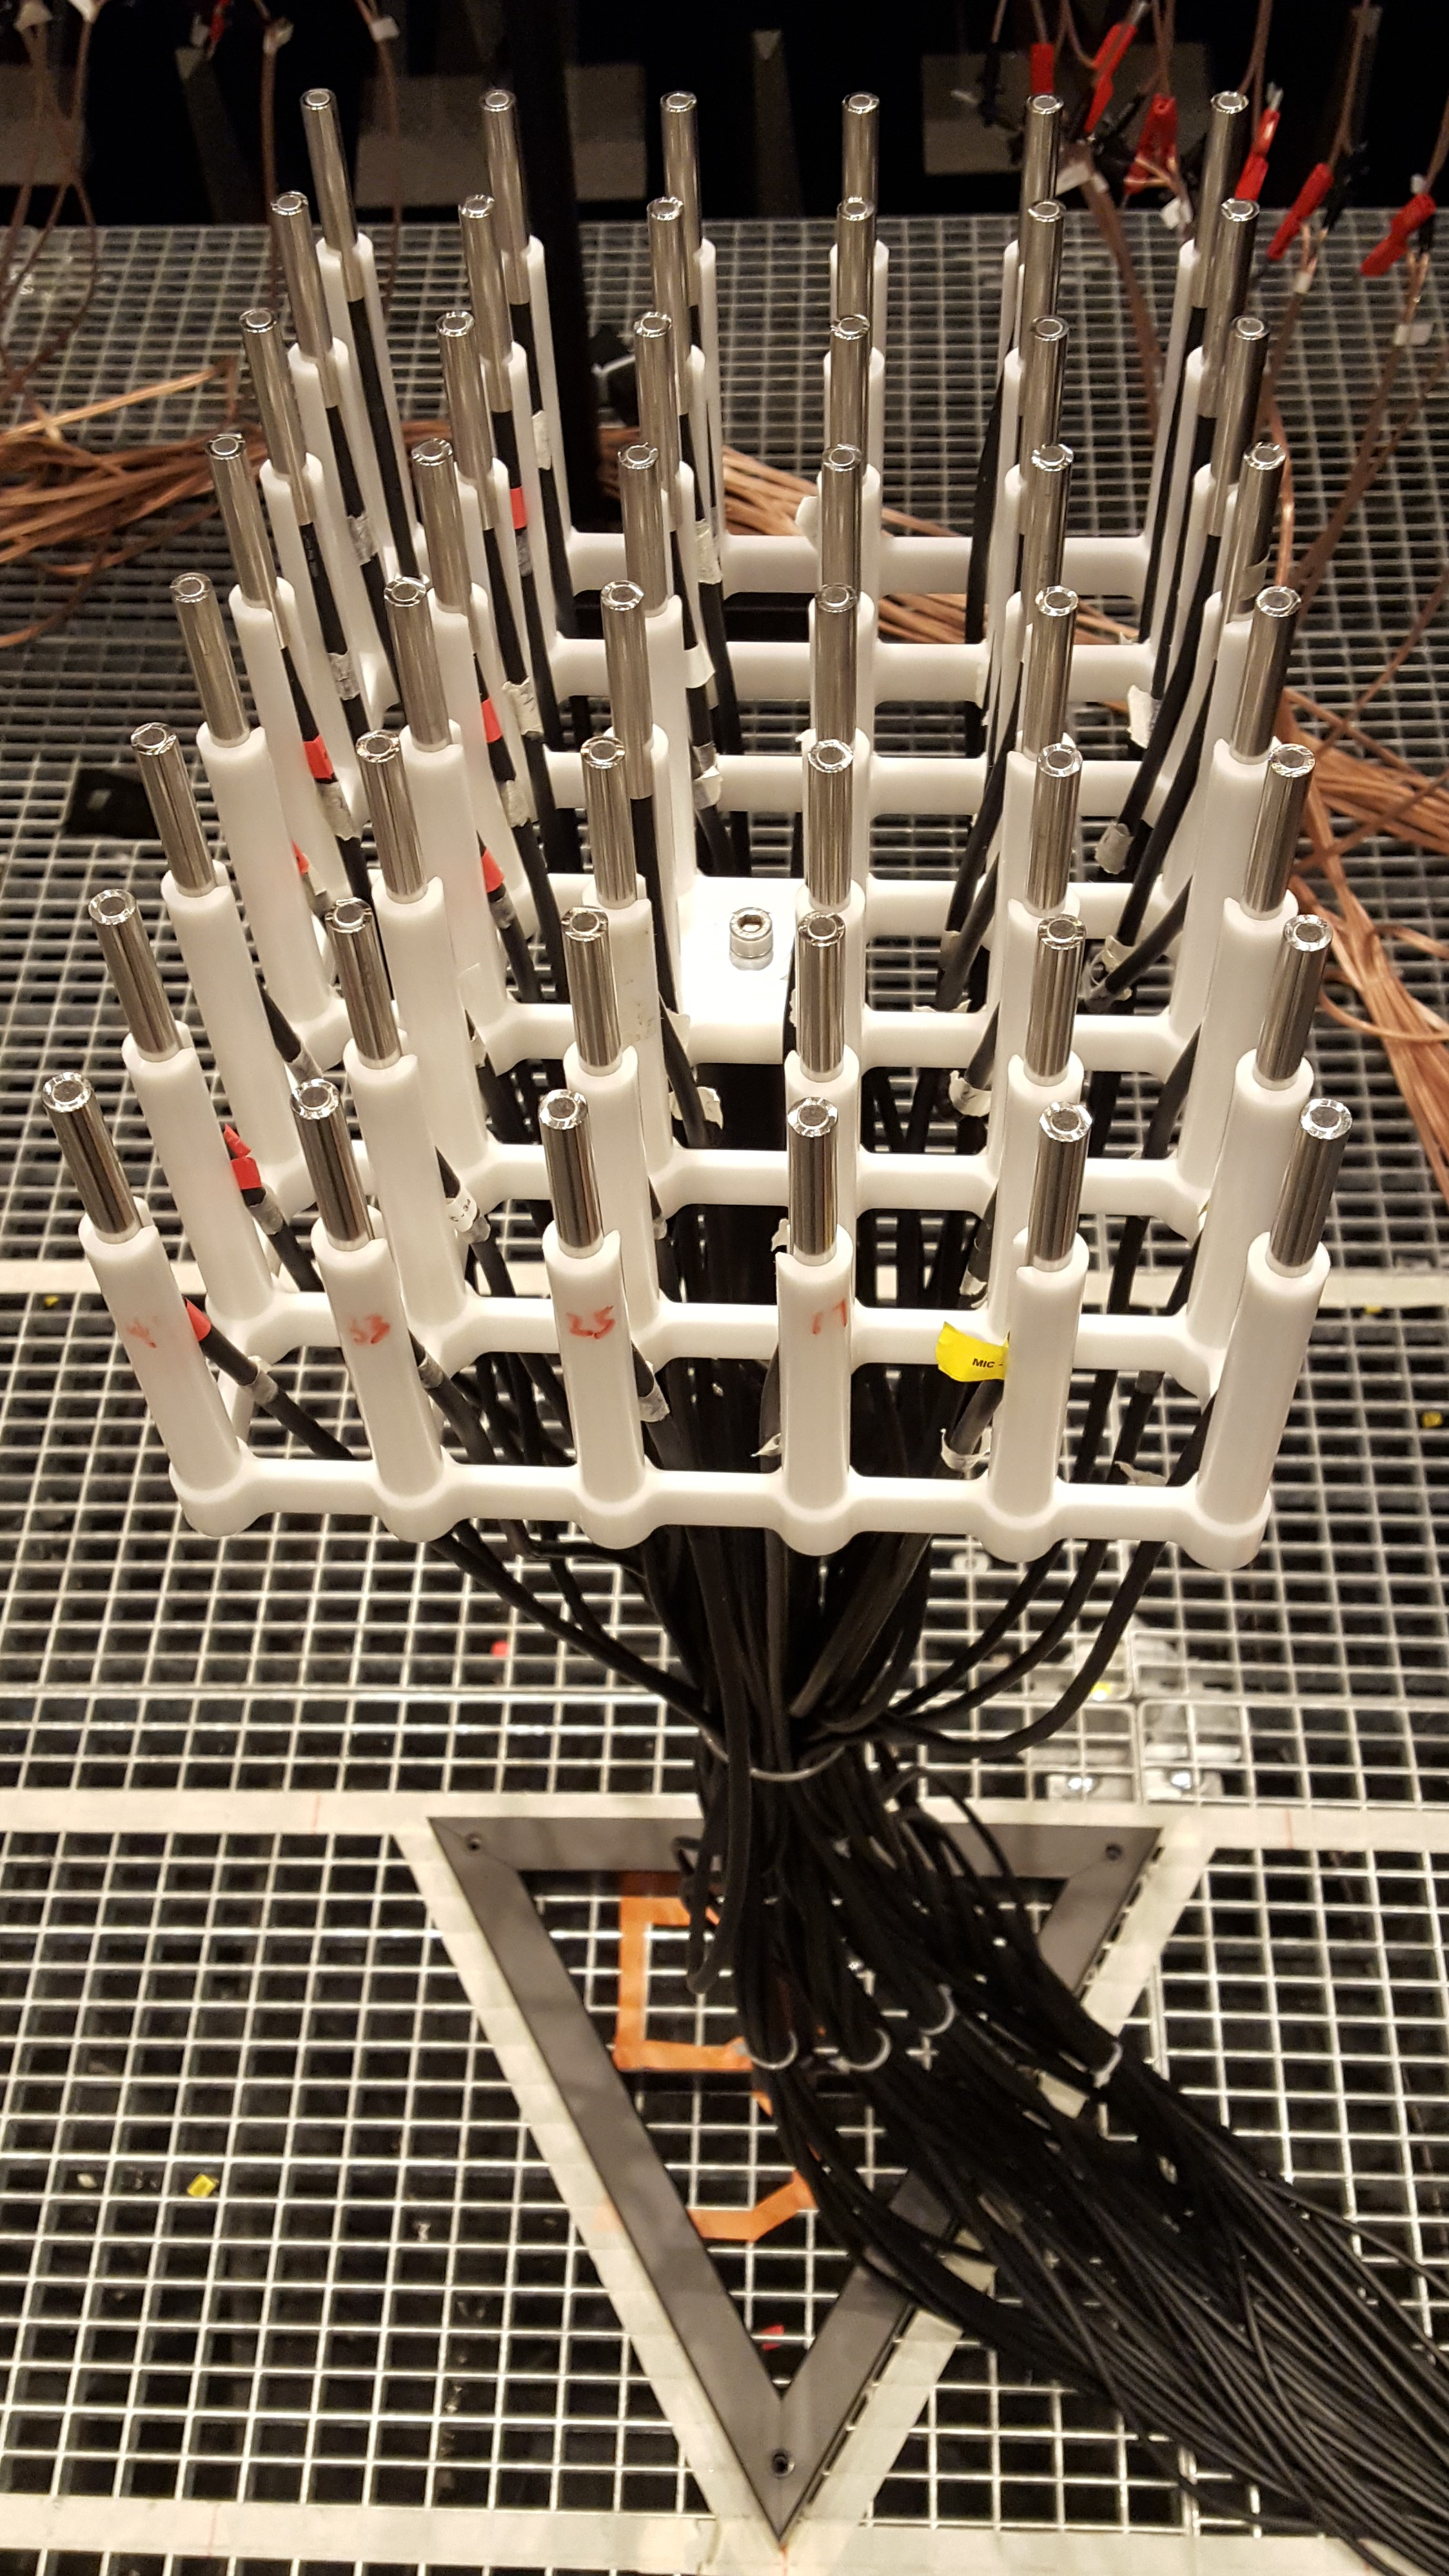
\includegraphics[width=10cm,height=10cm,keepaspectratio]{Figures/mics}
\decoRule
\caption[Microphone array with stand]{Microphone array with stand. the tape on the floor indicates the position of one of the two sound zones (the bright one in this case).}
\label{fig:mics}
\end{figure}

The distance between the microphones constitutes an higher limit to the sound frequencies that can be controlled. This is because of well known phenomenon of spatial aliasing, or grating.
\\
A soundwave should be sampled at more than two points per wavelength, otherwise the wave arrival direction becomes ambiguous. Having a distance $d$ of 5cm means that grating occurs at frequencies over $f = c/d \simeq 6.8$kHz, where c is the speed of sound ($343$ m/s in standard conditions). This value gives an ample security margin before the physical diameter of the microphones ($0.6 cm$) starts becoming a factor, in other words, the microphones can be considered detection points by the algorithm. 
\\
\\
Unfortunately, $6.8$kHz is not the upper limit before the grating effect appears. The relative angle between the center of the microphone matrix and the center of the loudspeakers array is another variable to take into account when defining the signal band. \parencite{cai_time-domain_2014} gives us the formula for the spacial aliasing, that is

\begin{equation}
f_{up}=\frac{c}{d(1+|sin \theta|)}
\label{eqn:freqaliasing}
\end{equation}

Where $c$ is the speed of sound, $d$ is the distance between the two centers and $\theta$ is their angle.
\\
Using the equation above, we find that $f_{up} \approx 2.9$kHz.
\\
\\
The SB speaker are divided in three arrays, each one having 12 driver units. The array at the center is the one used for the ACC experiments (speakers 13 to 24), while speakers 6 to 12 were briefly used for the experiment explained in section ~\ref{subsec:sbchoosing}. The central array was the one chosen for the experiments following the first one, because of its equal distance between the two sound zones, this causes a more balanced spread of the control effort undertaken by the single driver units.

\begin{figure}[H]
\centering
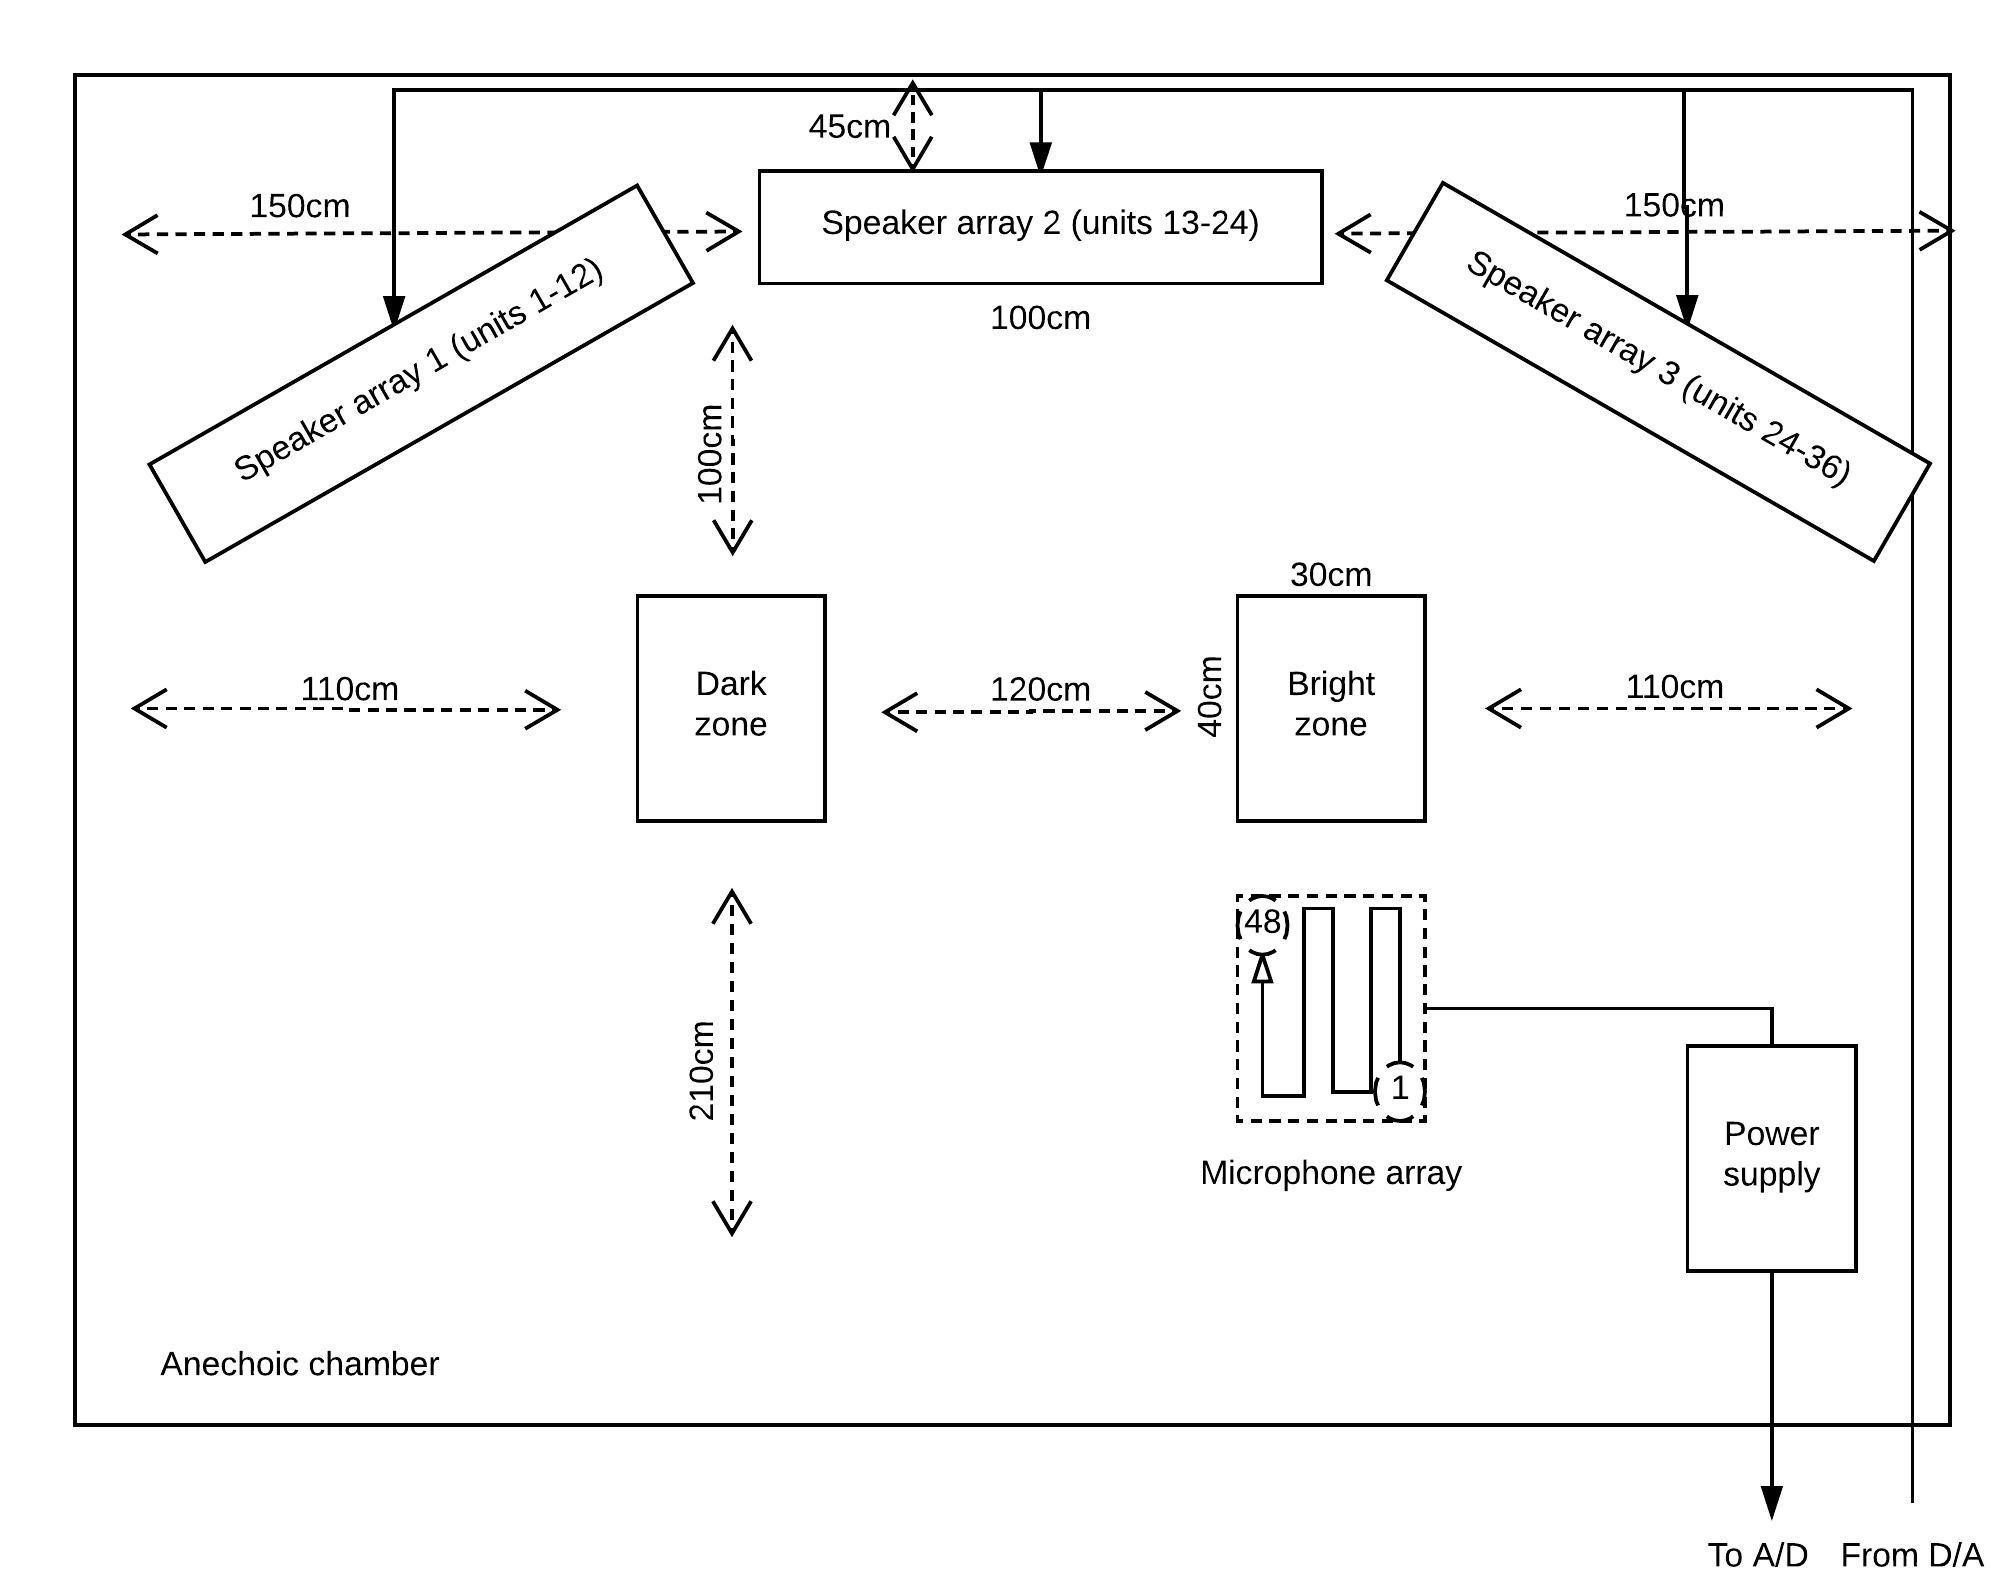
\includegraphics[width=14.5cm,height=15cm,keepaspectratio]{Figures/anechoicsetup}
\decoRule
\caption[Anechoic chamber setup]{The anechoic chamber setup.}
\label{fig:anechoicsetup}
\end{figure}

The presence of the other two arrays is justified by the fact that the room is also used for other experiments. The half-moon shape of the 3 arrays was chosen because the profile of the cabinets that causes reflections of the soundwaves is very limited. Since their impact in the contrast figure is minimal, it was not necessary to remove the units from the chamber.

\subsubsection{Listening room setup}

The microphones used in this scenario are mounted on a custom wooden frame, attached to a microphone stand. The microphones are positioned in circle. This was done to make sure they all had the same distance relative to each other.

\begin{figure}[H]
\centering
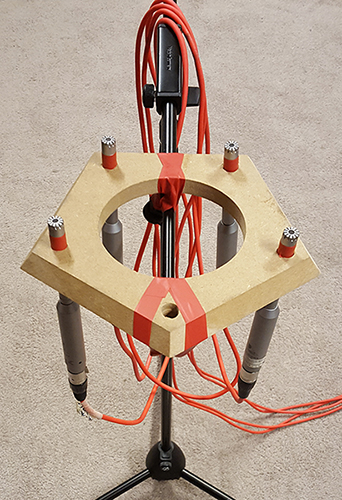
\includegraphics[width=8cm,height=8cm,keepaspectratio]{Figures/micslistening}
\decoRule
\caption[Microphone array in the listening room]{Microphone array with stand in the listening room.}
\label{fig:micslistening}
\end{figure}

In this case the frame has been carved out in the middle to limit the mechanical vibrations that high amplitude sounds might induce. Only four of the five microphone slots have been used, this is due hardware limitations in the input lines of the Fireface UC A/D converter.

\begin{figure}[H]
\centering
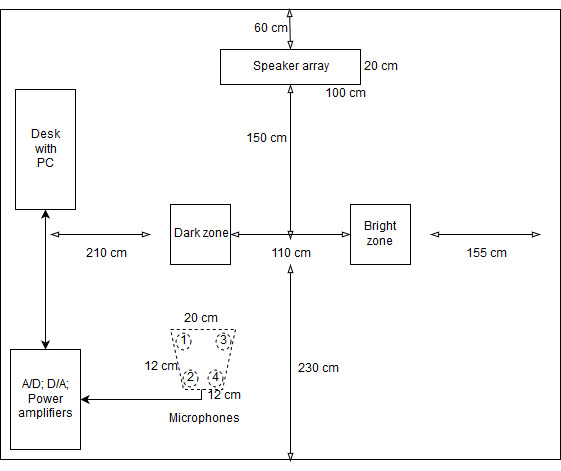
\includegraphics[width=13cm,height=12cm,keepaspectratio]{Figures/listeningsetup}
\decoRule
\caption[Listening room setup]{The listening room setup.}
\label{fig:listeningsetup}
\end{figure}

Finally, Using equation \ref{eqn:freqaliasing}, the upper frequency limit is $f_{up} \approx 3$kHz.

\subsection{Reflective surface}{}
\label{subsec:reflector}

The reflective surface used for the second part of the experiments is a plexiglass panel, mounted on a wooden frame. The panel dimensions are $125\textbf{x}105$cm (height and width), its thickness is $5.5$cm. The frame was realized by myself.

\begin{figure}[H]
\centering
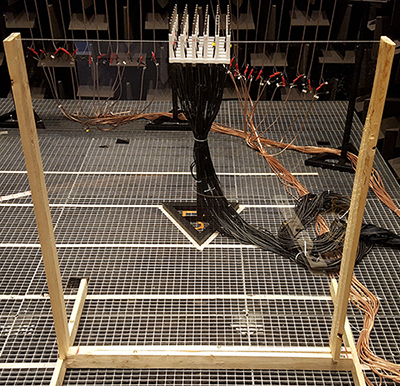
\includegraphics[width=8cm,height=8cm,keepaspectratio]{Figures/ref}
\decoRule
\caption[Reflective surface]{The reflective surface inside the room.}
\label{fig:refsurf}
\end{figure}

The reader will soon see how the introduction of the panel inside the anechoic chamber modifies the IR of the latter. By measuring the distance between the first peak, which corresponds to the arrival of the first, or "direct" sound to the microphones, and the second one, which marks the arrival of the reflected wave. 

\begin{figure}[H]
\centering
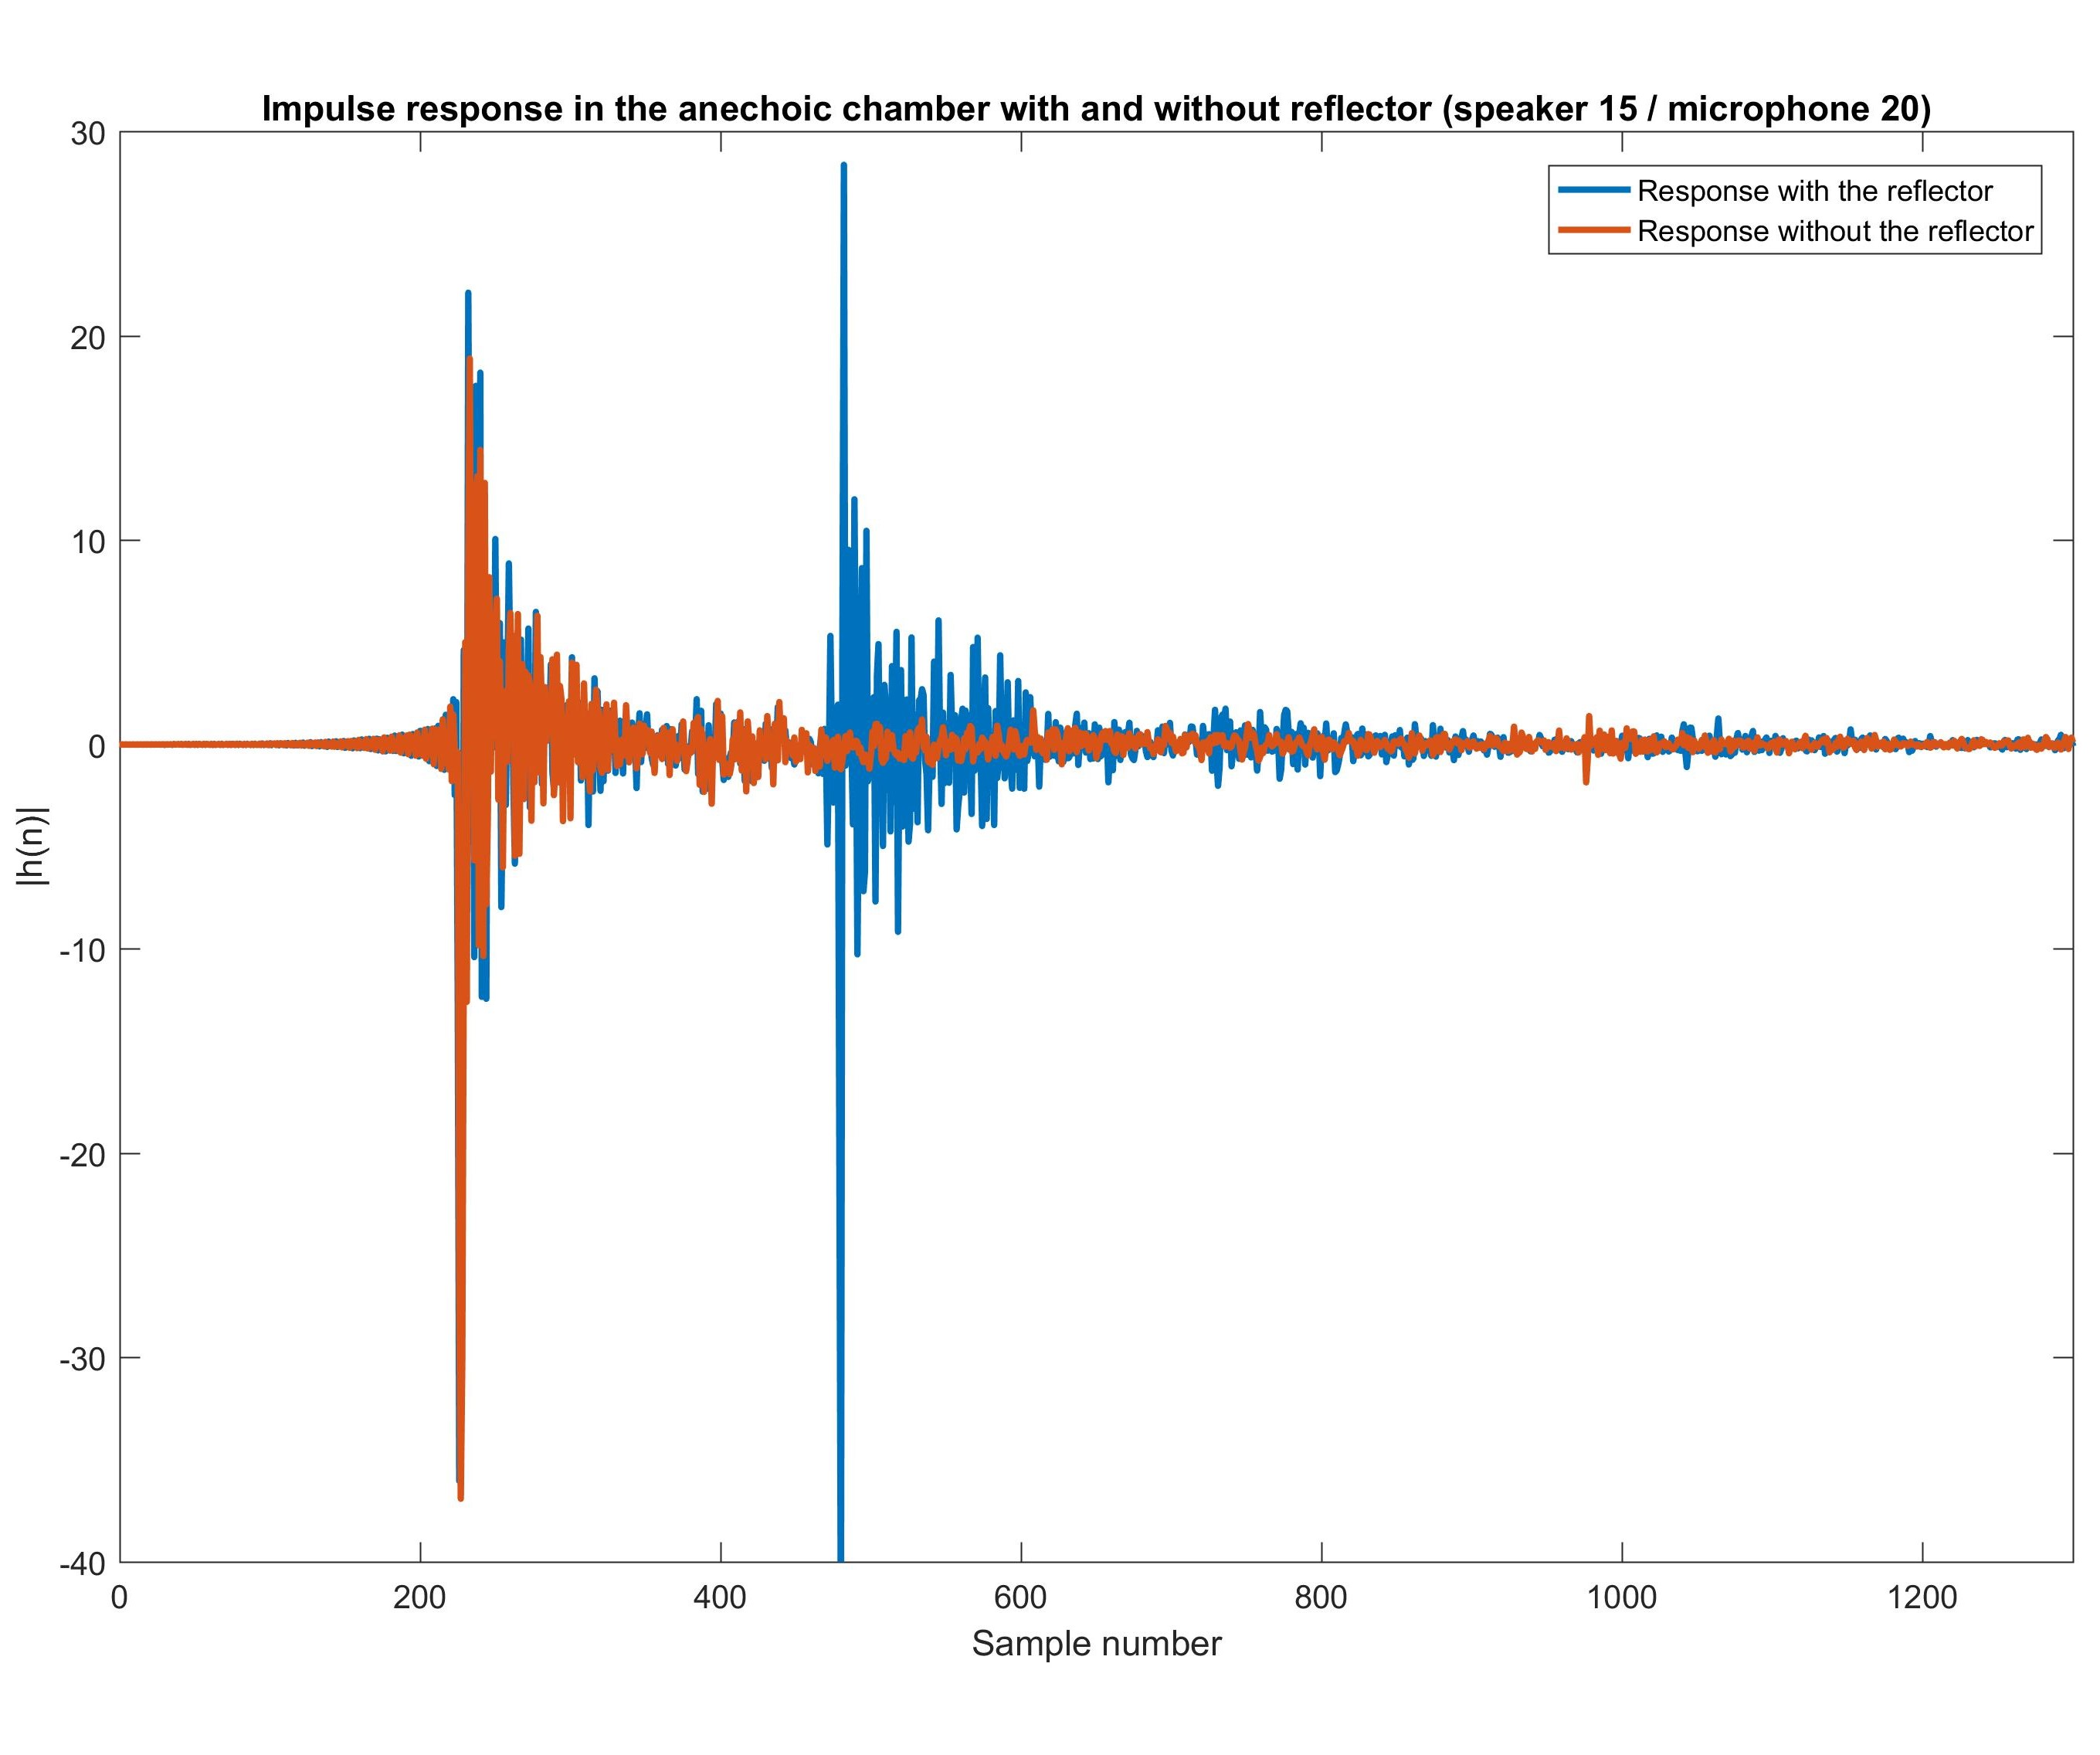
\includegraphics[width=14.5cm,height=15cm,keepaspectratio]{Figures/ir_ref_noref}
\decoRule
\caption[IR reflective surface]{Impulse response of the room when the panel is inside the room (blue line) compared to when it's not (orange line).}
\label{fig:irrefnoref}
\end{figure}

Please notice that the second peak has a bigger amplitude in the negative axis. This is because the direction of arrival of the reflection is opposite to the one of the direct wave.


\section{The signal chain}{}
\label{subsec:sigchain}

Once the desired digital signal is expressed in MATLAB and is sent to the computer's soundcard, by using the interfaces explained in section \ref{subsec:matlab}, it has to be converted in an analog signal, amplified and reproduced by the loudspeakers. In the meantime the resulting sound has to be recorded by the microphones.
\\
A schema representing the signal chain of the anechoic chamber is shown in Figure ~\ref{fig:signalchain}. Please notice that each box of the diagram represents an element where some kind of signal manipulation happens, like the conversion between digital, analog or mechanical domain. All the power amplifiers that, even tough scale the signal, do not change its domain, are omitted from the schema. In any case, both the loudspeakers and microphones are powered by such devices.

\begin{figure}[H]
\centering
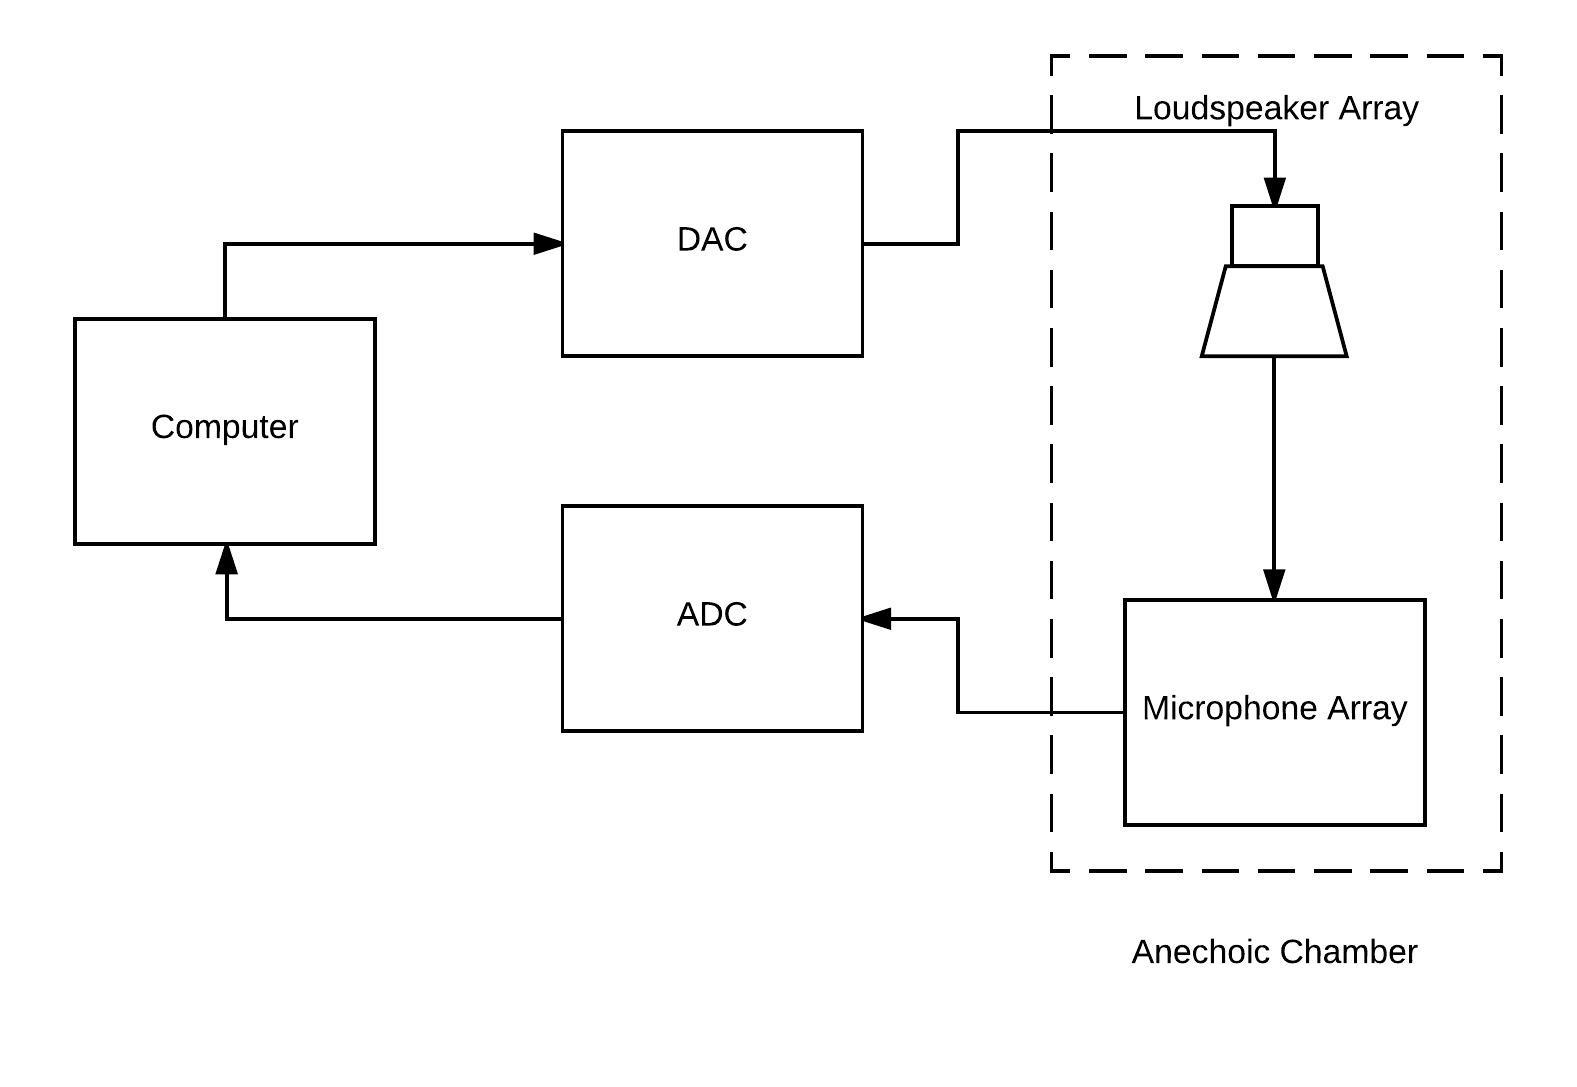
\includegraphics[width=12cm,height=12cm,keepaspectratio]{Figures/signalchain}
\decoRule
\caption[Signal Chain]{The signal chain.}
\label{fig:signalchain}
\end{figure}

The data lines for both the loudspeakers and the microphones are connected to the A/D converter units. One additional channel for both the elements is used for loopback. This means that they are not connected to an actual speaker or microphone, but rather they send data to the A/D input line, which mirrors it back to the computer trough its output lines. The purpose of this is to measure the delay that the converters introduce to the signal chain. Knowing this delay is very important, because it allows to synchronize the signal received form the microphones with the one sent out to the speakers. without it the filter calculated by the algorithm would not be convolved to the right samples, which means it would lose much of its effectiveness. Effectively, knowing this delay means that the first few samples recorded by the microphones have to be discarded. In most of the experiments run the loop delay is $\tld2200$ samples, with a sample rate of $48$kHz, which means it corresponds to $\tld0.046$s, which is in line with what can be reasonably expected by high quality of the instrumentation.
\\
\\
In the end, it has to be said that the signal chain in the listening room is identical to the one presented above, with the exception that all the instruments of the chain are situated inside the test room itself.

\chapter{Detailed experiments and discussion} % Main chapter title

\label{Chapter4} % For referencing the chapter elsewhere, use \ref{Chapter3} 

%----------------------------------------------------------------------------------------
\section{Measuring the speaker's harmonic distortion}{}
\label{subsec:sbchoosing}

The first step to achieve the objectives of the thesis stated in chapter \ref{Chapter1} is to decide the best alternative between the speakers that are available. The main parameter to take into account is the speaker's total harmonic distortion, which is a value that measures the percentage of power used by the driver unit to generate higher harmonics versus the power outputted at the fundamental frequency.
\\
As introduced in section \ref{sec:logsweep}, the best way to have a comprehensive analysis, in the whole frequency range of interest (corresponding the one the human ear is capable to perceive), [20-20000]Hz, is to use the Logsweep method to derive the impulse/frequency response of the speakers and evaluate which between the SB or Aura units gives us the best compromise.
\\
\\
It has to be said that the two speakers have a fundamental difference. The SB speakers were mounted inside a wooden cabinet (figure \ref{fig:aurasbspeakers}) filled with $5.8\pm1\%$g of glass wool. The insulator material has been put inside the frame in order to dampen the reflections coming from the back of the structure. The Aura array lacked such dampening. In order to make sure the comparison was "fair", meaning the two units were working at the best of their capabilities, without the cabinets interfering too much in the frequency response, the distortion caused by the Aura's cabinet needed to be measured and corrected.
\\
Moreover, the placement of the arrays was also a source of concern. It has already been said how the SB units are positioned onto some stands strapped down to the floor. The relatively big mass of the cabinets and its securing to the floor left little concern regarding the possibility that the measurements could be affected by mechanical vibrations of the stands. Concern that was instead present for the Aura unit, that has a much lighter frame. Additionally the cabinets themselves are a source of reflections and while the relative position of the SB units with respect to the microphones was chosen to limit the noise created by the cabinets, we needed to make sure that the Aura unit measurements weren't "contaminated" by the presence of such objects in the room. 
\\
In order to address this concerns the Aura unit has been positioned on top of the SB array (figure \ref{fig:aurasbspeakers}), which is the one on the left side of the room (figure \ref{fig:anechoic}).
\\
\\
The first experiment regarding the Aura unit consisted in choosing a good configuration with which measuring the harmonic distortions.
A Logsweep signal has been outputted to each one of the Aura speakers in the array to make sure all the drivers had relatively similar frequency response. Once we made sure all the units were functioning correctly, we could measure the effect the frame had. After some acoustic foam was made available by the laboratory, we could fill the Aura unit with appropriate dampening material and compare the frequency response of the two configurations.
\\
It was decided that having $10 \pm 1\%$g of acoustic foam inside the cabinet improved the frequency response, by improving I mean that the response presented less harmonic distortion, hence was more desirable. The foam going into each tube was weighted with a four digit precision scale, the tubes filled with the material can be seen in figure \ref{fig:aurasbspeakers}.
\\
\\
The microphone used for measuring the harmonic distortions was the Nti M 2010. The distance between the two set of speakers and the microphone was $\tld 1$m. Since the distance between the first and last speaker of each one of the two arrays is $43.5$cm for the Aura and $41.5$cm for the SB (center to center), the position of the microphone was adjusted to be facing directly the cones before taking each measurement. This was done to make sure that the increased directivity of the radiation pattern (section \ref{sec:soundgen}) could not invalidate the measurements.
\\
The code implementing the Logsweep was originally provided by the thesis supervisor and is among the codebase made available by the AUDIOLAB facilities of the Aarhus University. Some parts of said code have been adapted to better suit my needs while working on this thesis.
\\
Once the frequency response of both the loudspeakers were estimated, the harmonic distortion of each unit could be compared.
\\
\\
The microphone used for this measurement was the Nti unit.
The graph presents the results in relative scale of the distortion of the first Aura speaker (unit 1) and the leftmost SB unit used (speaker number 7), those were tested at relative volumes of $-30, -20, -10$ (which means $75.0, 85.1, 94.4$dB for the SB and $72.0, 81.5, 90.6$dB for the Aura). Having the same output levels makes sure that the input signal for the drivers is identical in both cases.

\begin{figure}[H]
\centering
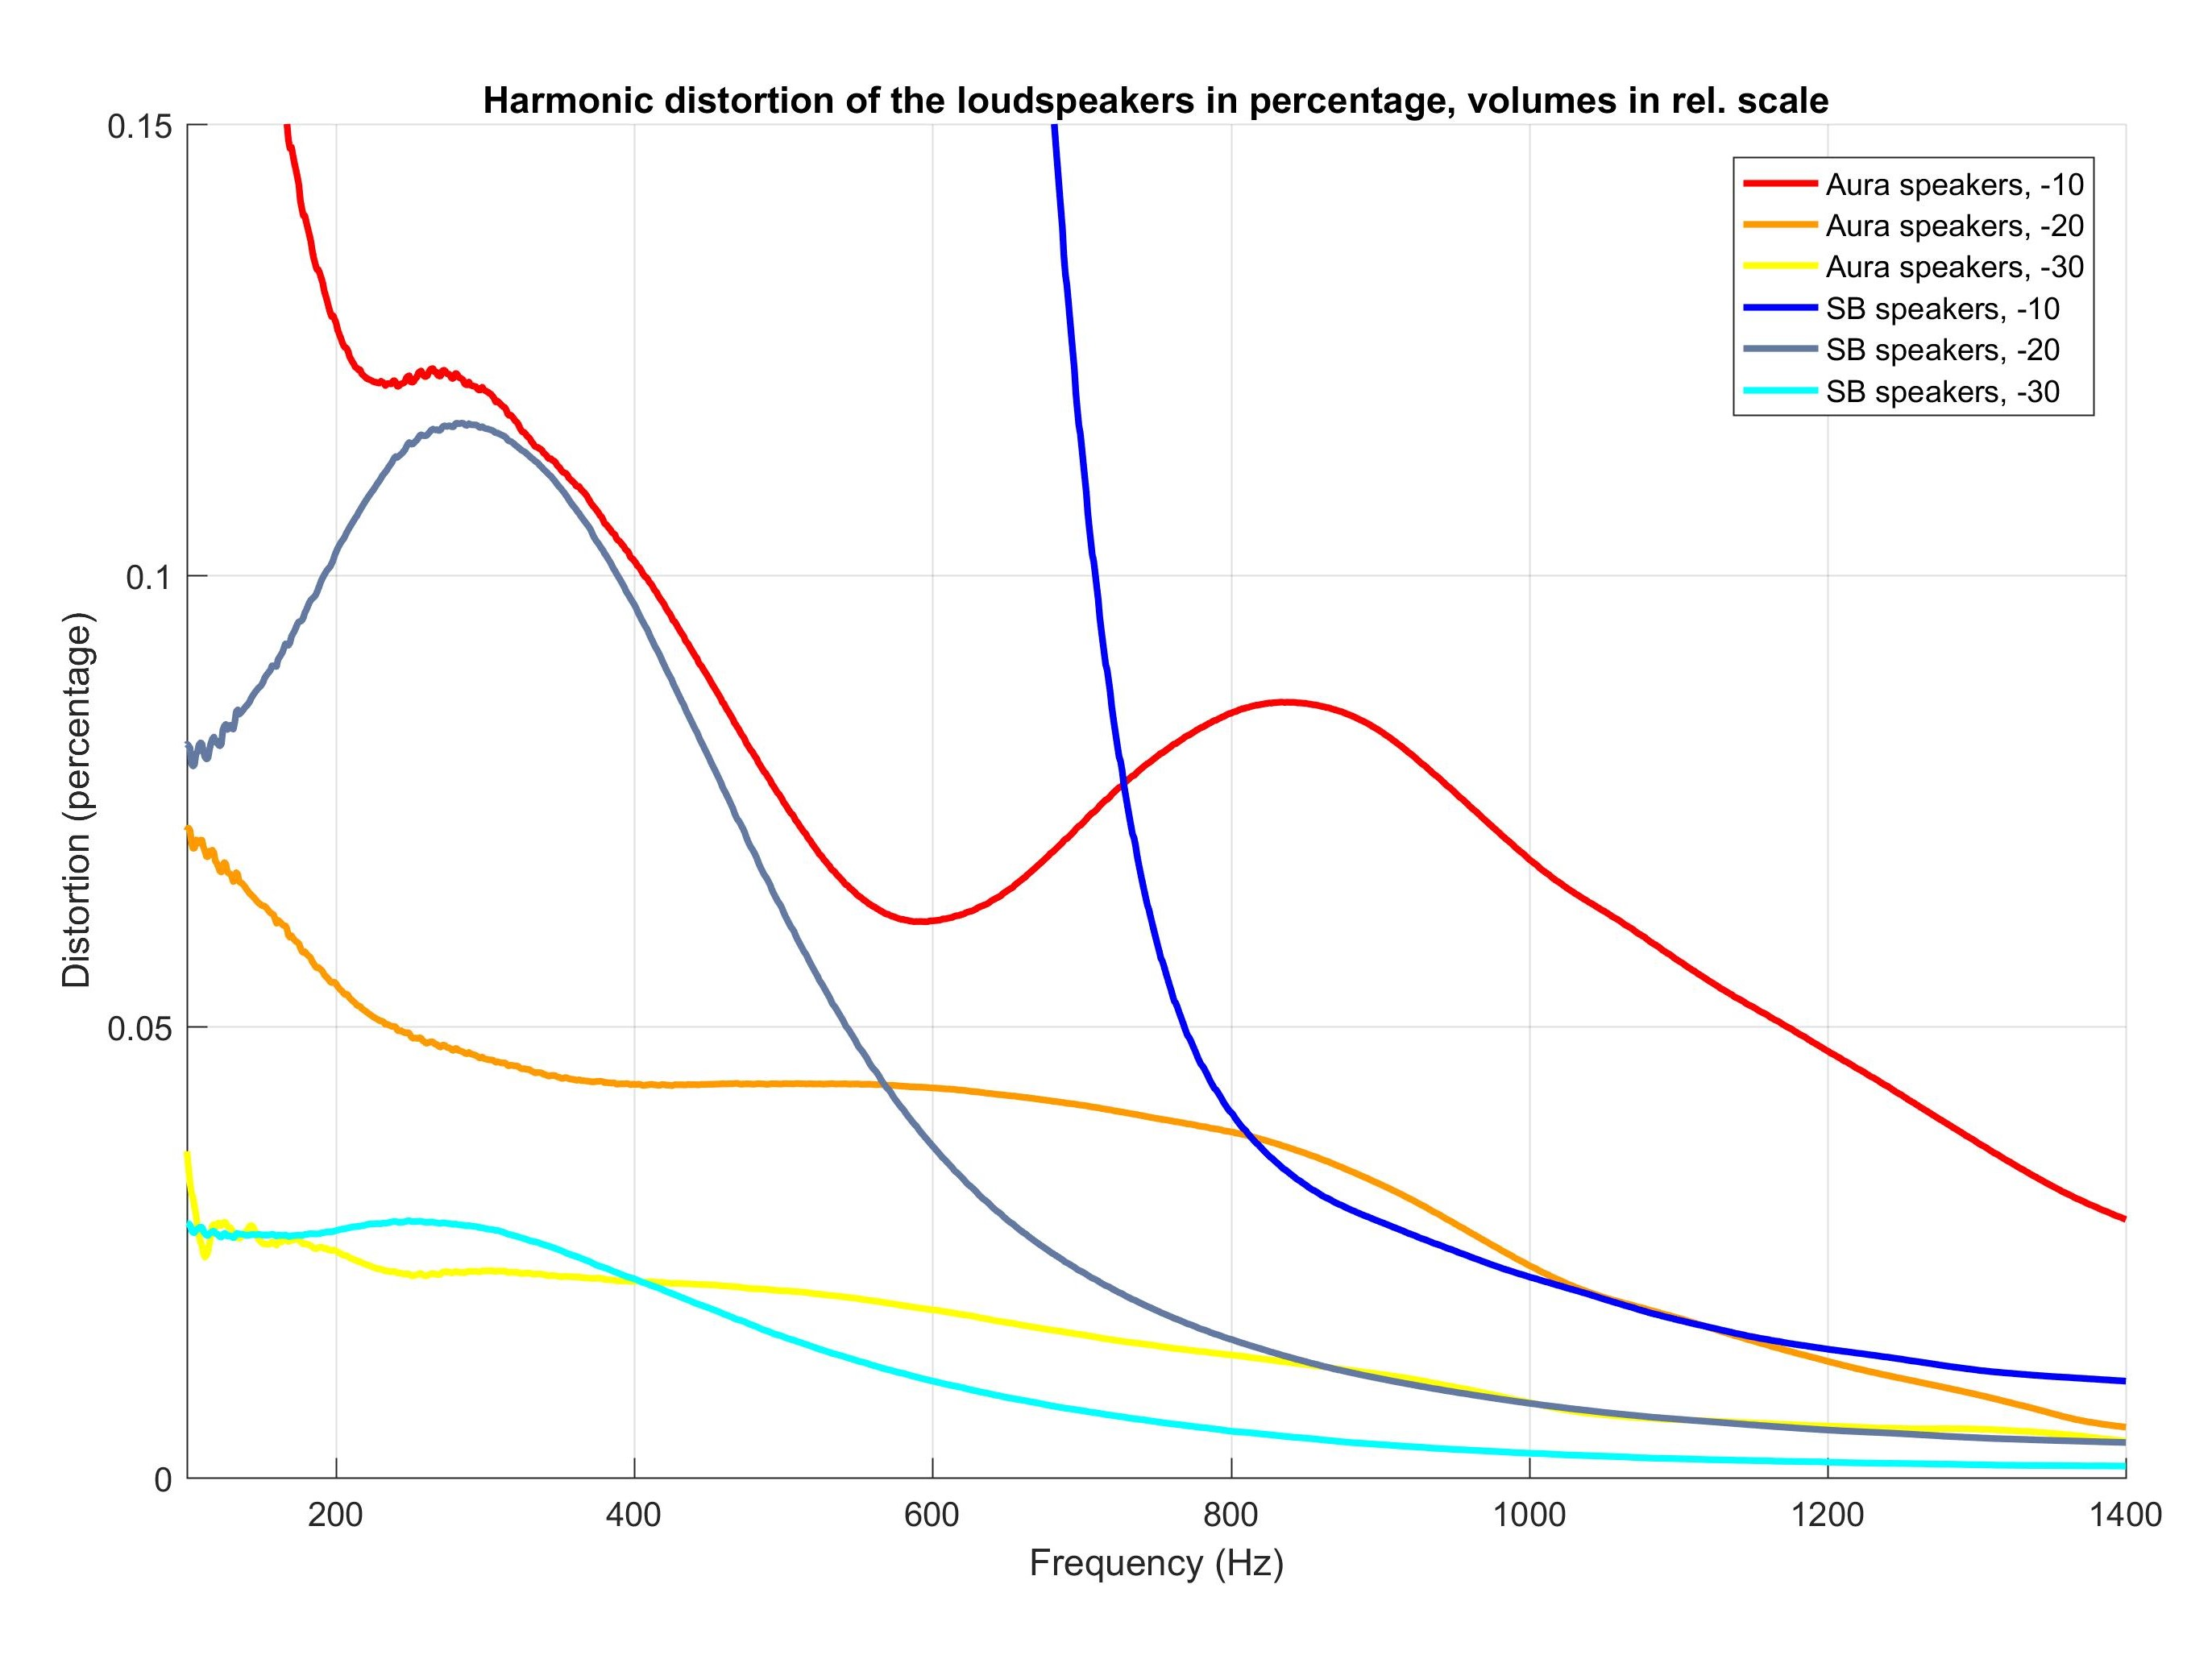
\includegraphics[width=14cm,height=14cm,keepaspectratio]{Figures/harmonicdistortion}
\decoRule
\caption[Harmonic distortion of the two loudspeaker models.]{Harmonic distortion of the two loudspeaker models. Lower is better.}
\label{fig:harmonicdistortion}
\end{figure}

The value in the vertical axis represent the amount of power, in percentage, that ends up generating a nonlinear response. This value was calculated using the formula

\[\frac{\Re\left(H_2(f)\right) + \Re\left(H_3(f)\right)}{\Re\left(H_1(f)\right)}\]

Where $H_1(f)$, $H_2(f)$ and $H_3(f)$ are the first, second and third harmonics of the system. The $\Re$ symbol is the real part of the complex number. The horizontal axis represents the frequency.
\\
This experimental result presented in the graph above is in agreement with what discussed in section \ref{sec:soundgen}. Seeing that the harmonic distortion increases when lowering the frequency is, in fact, what we discussed when talking about harmonic distortions.
\\
\\
As it can be seen from the figure above, higher outputs cause the generation of more nonlinear distortions at all frequencies, even though this effect is more prominent in the lower part of the frequency spectrum ($<500$Hz).
\\
This experiment shows some interesting results. Even though the Aura unit shows lower distortion at low frequencies, crossing over the $750$Hz range the SB speaker appears relatively better, especially when playing sound at lower power levels.
\\
As the reader can see, frequencies over the $1$kHz mark, create very little nonlinearities, especially when using the SB unit, which has a $2\%$ of distortions, even when playing at relatively higher volumes. 
\\
\\
After this analysis, it is possible to determine the unit that better suits our needs for the remainder of this project. As stated in section \ref{Chapter2}, an upper frequency limit was set by the formula \ref{eqn:freqaliasing}, so we already know that the upper bandwidth of the signal will be $2.9$kHz, while we can choose the lower band as we please, trying to stay in the most linear part of the system, since it is the only order of the system that is controlled by the algorithm.
\\
At this point of the project, it was impossible to know the target output level when performing the BACC-RD experiment, but it was clear that playing at lower volumes would have improved the contrast figure.
\\
\\
The model of loudspeakers chosen for the following tests was the SB array. Even though the frequency response of the Aura units is better at low frequencies, the fact that the following experiments could be performed without changing the setup in the room was considered an advantage that overcomes the slightly worse response. If played at an output level (in relative scale) of $-20$ or lower, the harmonic distortion of the SB speakers is $10\%$ at $\tld 300$Hz and it rapidly drops below $5\%$ at $\tld 550$Hz, which can be considered low enough to not disturb the contrast generated by the BACC-RD algorithm (and its later variations).
\\
Moreover the laboratory had a supply of spare loudspeaker units available and an entire, unused, array. It would be later used to reproduce the contrast experiment in the listening room.
\\
The lower frequency limit can be adjusted to best suit our needs, knowing that signal with high powers below the $\tld 300$Hz mark will impact the contrast figure in an heavy way.
\\
Finally, we confronted the SPL generated by each speaker array when all the units in question are playing.
To get this measurement we used all eight the drivers from the Aura unit and speakers 7 to 12 for the SB array. Using the microphone matrix and positioning it at $1$ meter from the center of the array of the speakers used, and outputting the same level, in relative scale, of $-20$, the measured Sound Pressure Level (SPL) was $95.5$dB $\pm0.2$dB for the Aura unit and $94.5$dB $\pm0.2$dB for the SB speakers. This sound level was made by averaging the SPL values of microphones $20, 21, 28, 29$. Each of these measurements was repeated five times.
\\
\\
Now that the properties of the speakers are well known, it is time to start reproducing the results of \parencite{cai_time-domain_2014}.


\section{Applying the BACC-RD method}{}
\label{sec:baccrd}

\subsection{BACC-RD in the simulated environment}{}
\label{subsec:baccrdsim}

In section \ref{sec:simenv} we described the characteristics of the simulated environment. A simulation was needed to debug the BACC algorithm and to quickly change the speakers/microphones/soundzones configuration, in order to get some familiarity with the whole process. Testing the algorithm in a simplified environment greatly sped up the code development by giving the possibility to test the algorithm without having to deal with the underlying hardware. 
\\
\\
Once the IR of the simulated room was proved to be reasonable (figure \ref{fig:simir}), it was given to the BACC algorithm, which would use it to calculate the $R_b$ and $R_d$ terms for equation \ref{eqn:lagrange}. The parameters of the Lagrange maximization problem were set as $\beta = 0.5$ and $\delta = 10^{-6}$ (These are the regularization terms of equation \ref{eqn:lagrange}). The choice of these particular values was made to compare, as we will later see, the eventual contrast figure with the results of \parencite{cai_time-domain_2014}.
\\
At the end of the algorithm, an optimal solution to the Lagrange problem  of equation \ref{eqn:optimization}, in other words, a $w_{BACC}$ filter is returned.

\begin{figure}[H]
\centering
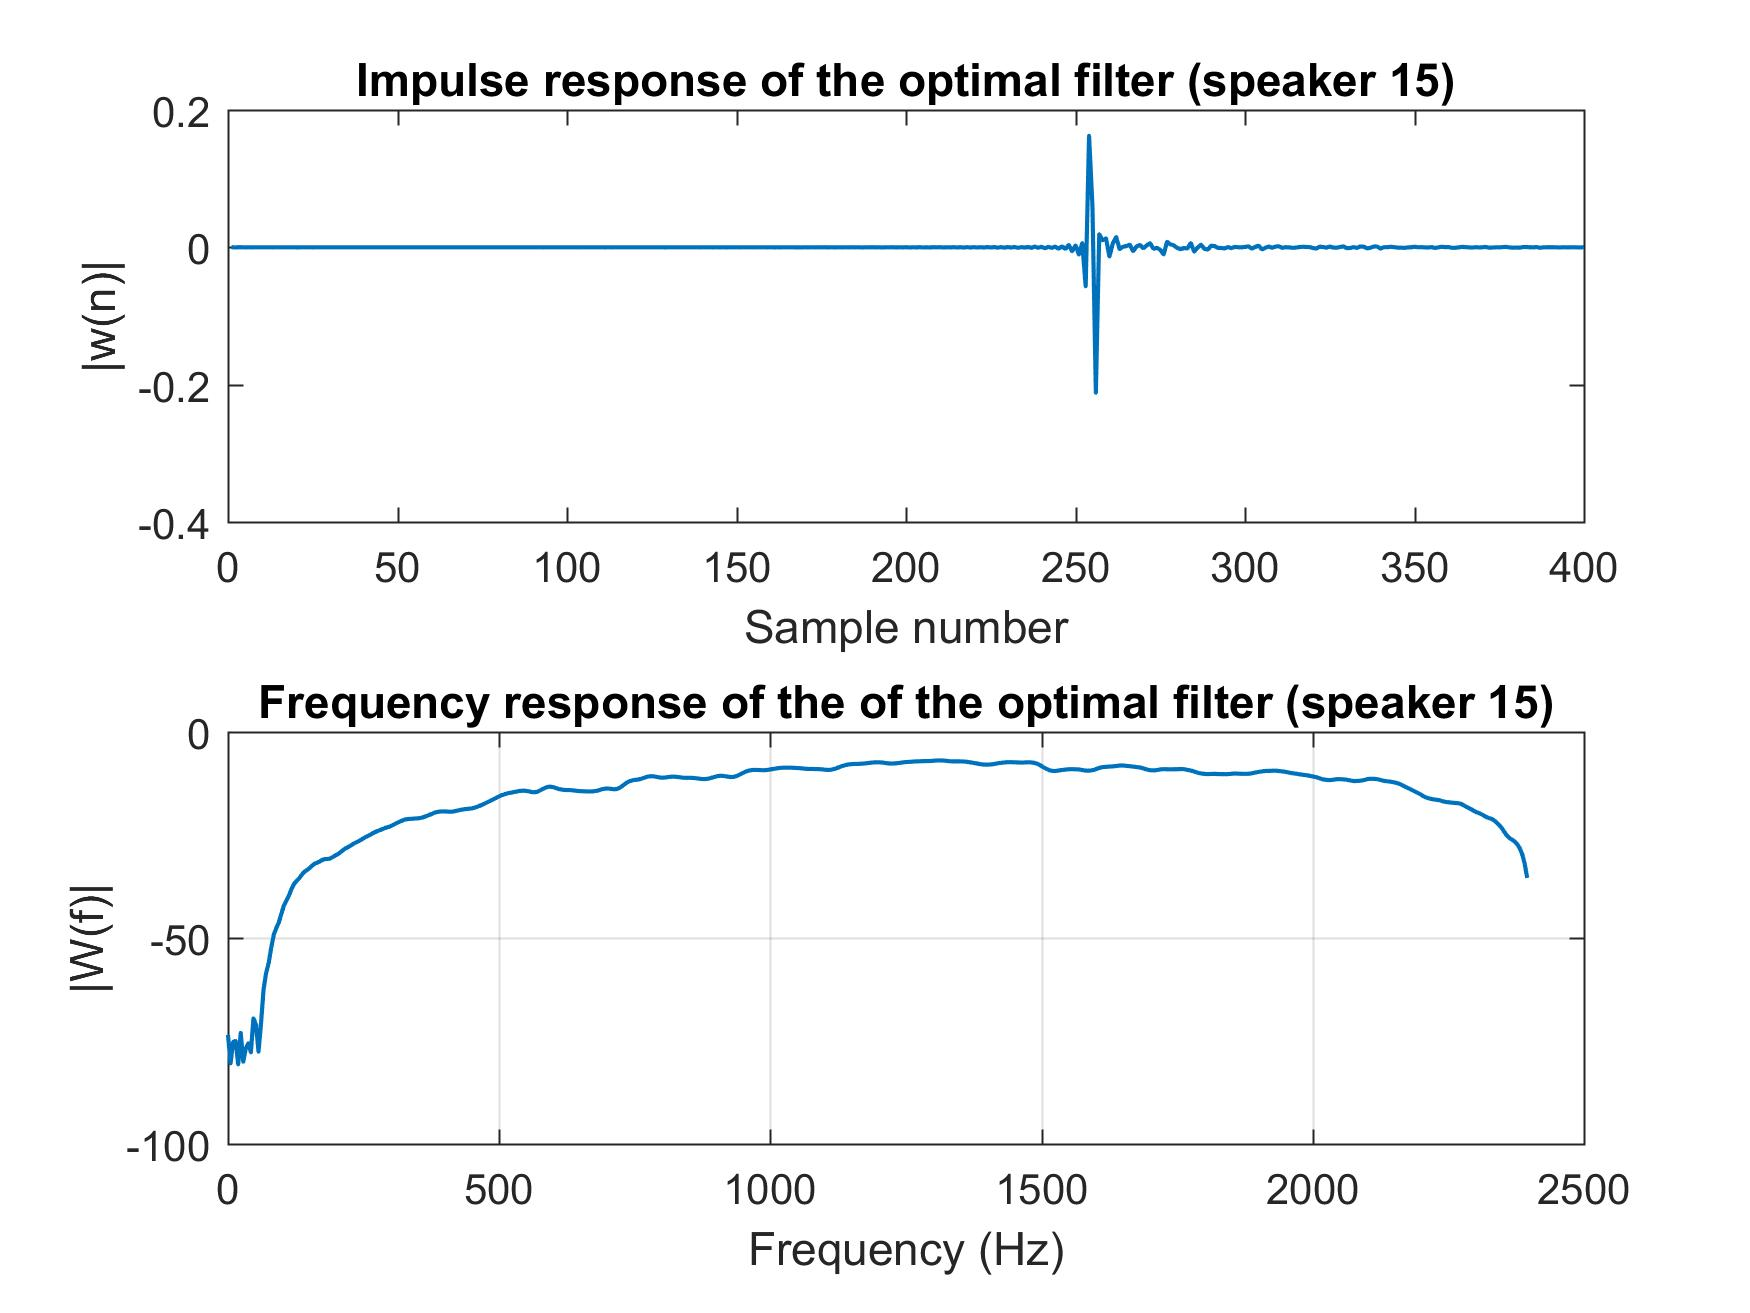
\includegraphics[width=13cm,height=13cm,keepaspectratio]{Figures/ir_fr_w}
\decoRule
\caption[Impulse and frequency response of $w_{BACC}$]{Impulse and Frequency response of $w_{BACC}$.}
\label{fig:ir_fr_w}
\end{figure}

The maximum contrast achievable can vary, even considerably, depending on the particular setup used. In section \ref{subsec:baccvary} we will see how the parameters influence the contrast figure.
\\
\\
Once the IR of the system was estimated, the harmonic distortion of each zone could be compared. This was done by performing the convolution between the simulated IR, the $w_{BACC}$ filter just calculated and a test signal.
\\
The test signal is white noise that has been band-passed in the $[500-2400]$Hz range. There is no particular reason why the frequency range of the signal, at this stage, is that particular one, but this is a similar range to the ones used when performing the experiments in the actual anechoic chamber, hence they can be an useful test bench. Of course the upper limit is limited by the sampling frequency chosen, which was $4800$Hz, but in principle, we could extend both indefinitely.
\\
\\
The algorithm automatically divides the range of the controlled frequencies in a series of equally spaced bins. The central values of these frequency bins will be the control frequencies, the points where the filter will generate the highest contrast, meaning that if we compare the frequency response of the system in the two zones, we will see the biggest excursion between the energy levels of the two ones at those specific control frequencies. By increasing the sampling frequency we are able to shorten the distance between the bins and better control the frequency response of the system, thereby increasing the contrast. A flat frequency response is something desirable because we will output an equal amount of energy in the frequency range of interest, therefore we will not alter the spectral properties of the signal that is being played.

\begin{figure}[H]
\centering
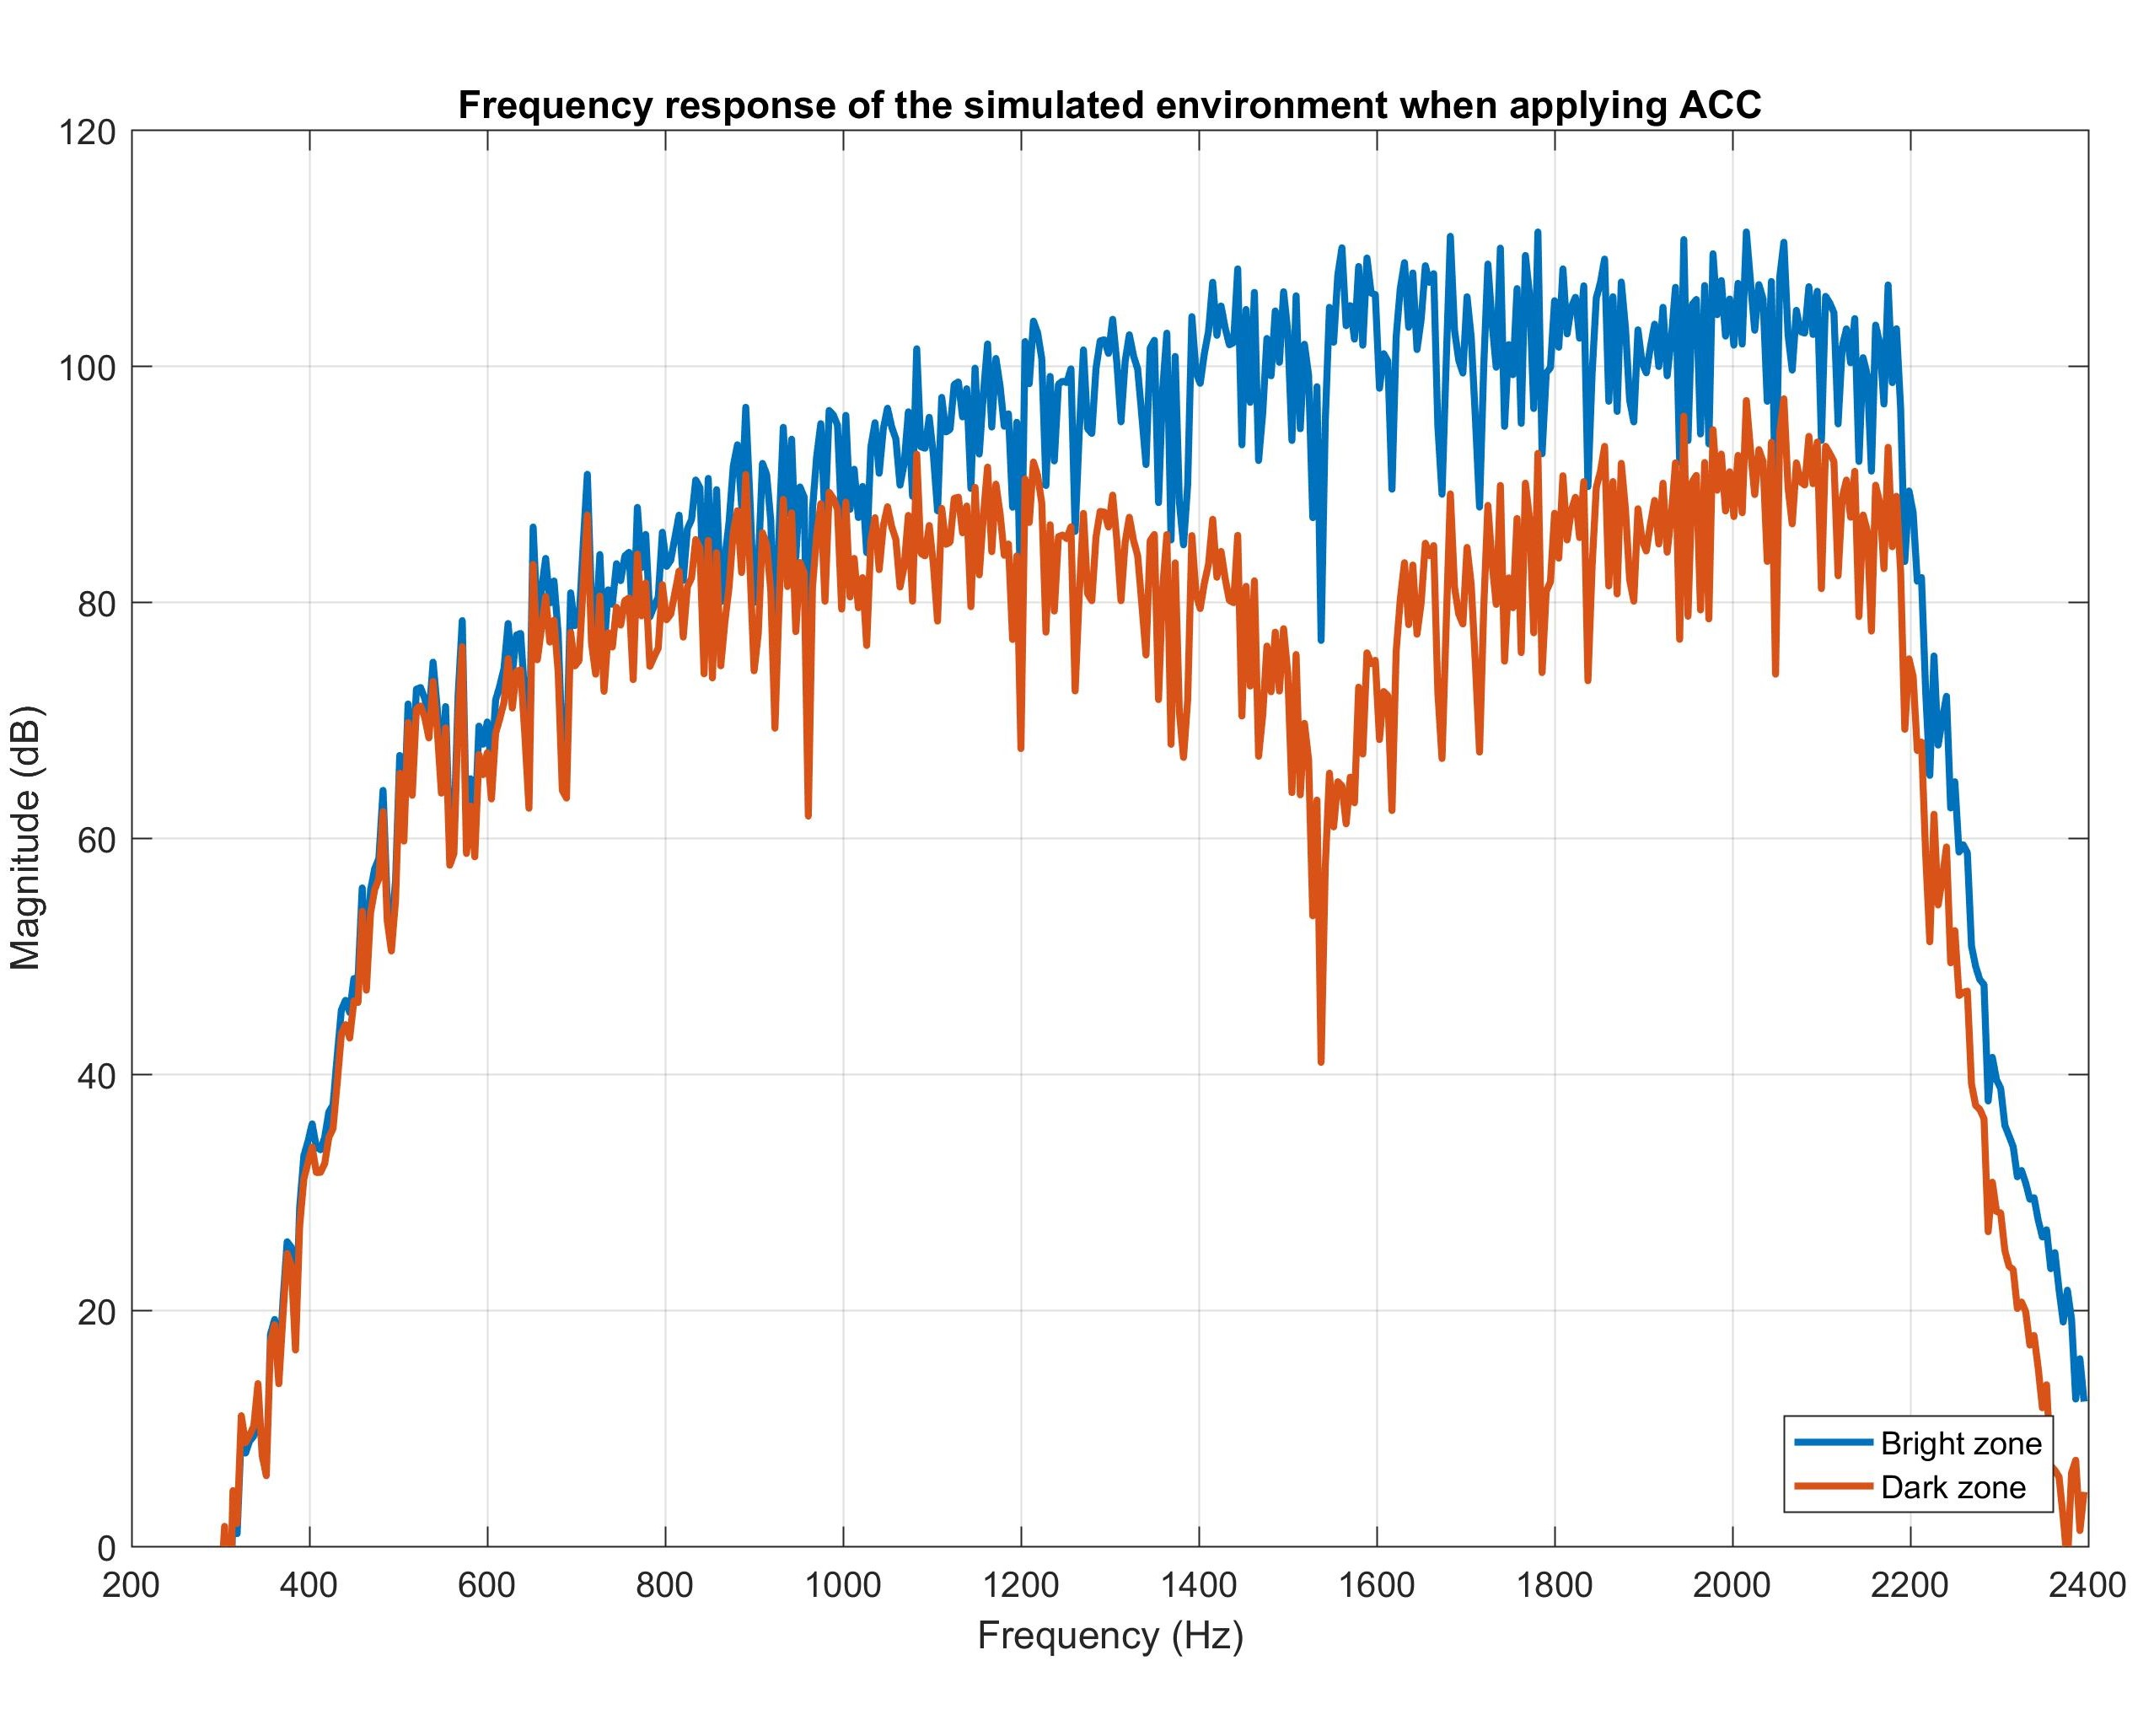
\includegraphics[width=14cm,height=14cm,keepaspectratio]{Figures/contrast_simir}
\decoRule
\caption[Acoustic contrast in the simulated environment.]{Acoustic contrast in the simulated environment. The curves represent the frequency response of the system in the top left microphone of the dark zone and the bottom left microphone of the bright zone from figure \ref{fig:simroom}.}
\label{fig:contrast_simir}
\end{figure}

The theoretical maximum achievable, with the specific room configuration (section \ref{sec:simenv}) and parameters presented above, using the simplified propagation model given by \ref{eqn:green} (which, again, produces the IR in figure \ref{fig:simir}), is $\tld 34.2$dB of acoustic contrast. The contrast figure varies every time we run the algorithm, because of the particular realization of the noise. The sample size generated by running the algorithm multiple times is too small to have a statistical analysis, but after five runs it appears that the contrast diverges from said value by $\pm3$dB.
\\
\\
Now that the algorithm has been tested and we can achieve some acoustic contrast, we could move the experiments in the anechoic chamber.

\subsection{BACC-RD in the anechoic chamber}{}
\label{subsec:baccrdanechoic}

The first step to realize acoustic contrast is to measure the room's IR. This is done outputting the Logsweep function in the frequency range of $[20-20000]$Hz. It is reminded to the reader that the code used for this section was been provided by the AUDIOLAB, later modified in some parts by myself.
\\
The speakers used for this and the rest of the experiments in the anechoic chamber are units 15 to 22 and not units 7 to 12, like the previous test regarding the harmonic distortion of the drivers. This was a deliberate choice, the reasoning behind this is that I originally thought of using different drivers in each of the available array, but the ACC algorithm, promoted higher power outputs coming from some loudspeakers rather than others, accordingly to the positioning of these units with regards to the sound zones. By standing in the bright zone one could clearly tell that the speakers on the right side of the room were playing more loudly than the others. I decided that this effect was unpleasant, so I ended up using the central SB array (units 15 to 22) for the rest of the experiments.
\\
This choice does not alter the results of section \ref{subsec:sbchoosing} in any way, since all the speakers show similar spectral characteristics.
Please refer to figure \ref{fig:anechoicsetup} for more details regarding the position of microphones and speakers used.
\\
\\
As anticipated in subsection \ref{subsec:mics}, the experiments had to be repeated twice, because there was only one microphone stand available. This has to be moved between the two zones. The reader should be aware that this fact introduces a certain degree of uncertainty when estimating the IR of the room. This is because when we are moving the stand from one zone to the other we are changing the response of the system.
\\
For example, let's say after performing the IR estimation with the microphones in the bright zone, we move the stand in the dark one, we are effectively modifying the IR of the room, which was estimated when having a source of reflections (even though small) in the first area, that has now been moved away. This uncertainty cannot be eliminated without adding a second stand with the same shape and working microphones, so that we could measure the IR in both zones at the same time. This, unfortunately, was not an option during the experiments.
\\
It has to be said, though, that this effect has been limited as much possible, by trying to limit the reflection that the various components of the stand introduce, using the specification discussed in subsection \ref{subsec:mics}.
\\
\\
Once the IR of the room is known, we can calculate the correlation matrices $R_b$, $R_d$ and the $RD$ term of equation \ref{eqn:lagrange}.
We have already seen in section \ref{sec:acc} that the filter and IR lengths are a parameter to take into account when calculating the solution to the contrast problem. The increase in length causes an increase in the size of $R_b$, $R_d$ matrices that goes with the square of the sum $M + I$ (filter length plus IR length), moreover this value has to be multiplied for each microphone-speaker pair.
\\
\\
Without going into the specifics of the code, if we decide, for instance, to have an IR and FIR filter lengths of $300$ samples each, using 8 loudspeakers and 4 microphones, we are looking at two matrices ($R_b$, $R_d$) of $5.76 \textbf{x} 10^6$ elements each; If we increase the number of samples to $600$, we will have twice $2.30 \textbf{x} 10^7$ elements. It appears clear how these magnitudes imply a huge amounts of calculations and even with the most powerful hardware available today, it makes finding the optimal ACC filter a rather slow process. For instance, with a 2012 Intel i7 2600K processor with 8GB of DDR3-1333mHz RAM, calculating a $600$ taps $w_{BACC}$ filter takes close to an hour.
\\
This result can vary with the hardware used and I don't exclude that performance improvements in the code might lead to faster results, but it appears clear that finding a balance between the number of samples and the algorithm's performance is very important in order to end up with a reasonable computational time.
\\
\\
In the figure below we can see a closeup of the IR of the anechoic chamber, calculated using microphone 20 and speaker 15. The microphones matrix was positioned in the bright zone.

\begin{figure}[H]
\centering
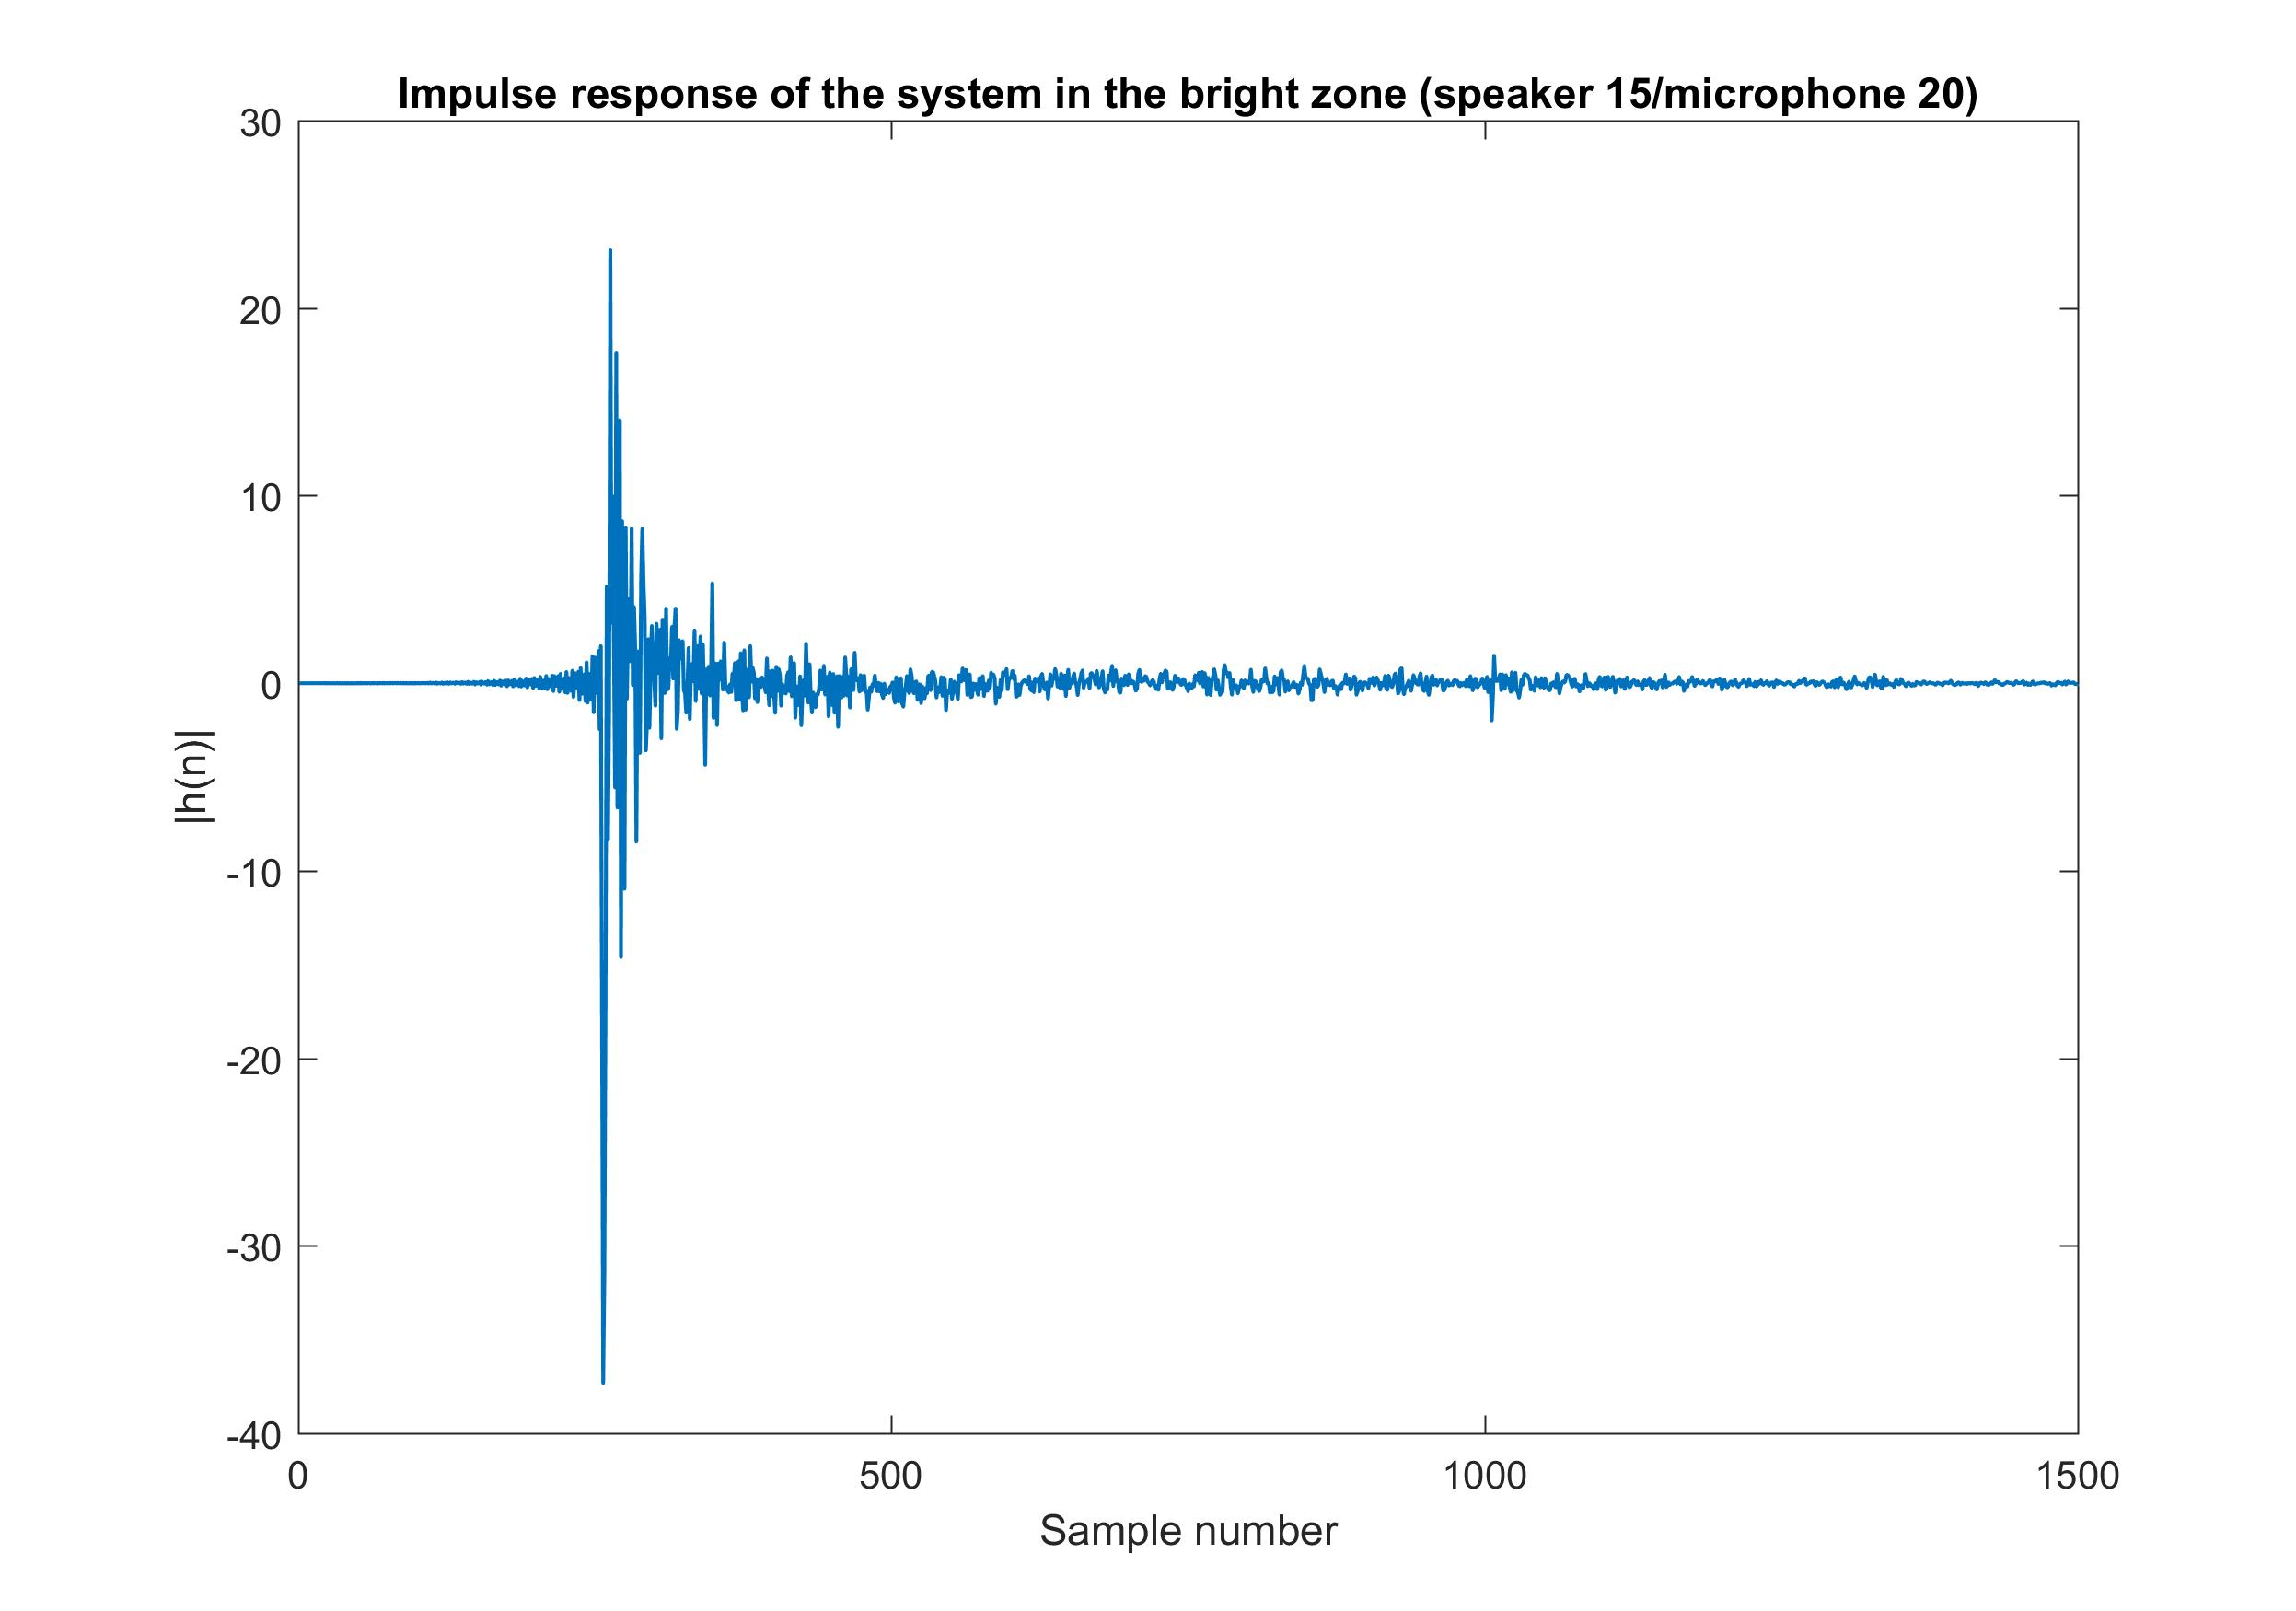
\includegraphics[width=14.5cm,height=14cm,keepaspectratio]{Figures/ir_bright}
\decoRule
\caption[Impulse response of the anechoic chamber]{Closeup of the IR of the system in the anechoic chamber. The measurement starts from the moment the first sound exits the loudspeaker under test. }
\label{fig:ir_bright}
\end{figure}

As already stated, the delay introduced by the hardware is omitted from the graph. The first $\tld 200$ near-zero samples are caused by the acoustic delay, which is the time the soundwaves take to reach the microphones. The measurement was obtained using a Logsweep signal for 10 seconds with $48$kHz as sampling frequency. 
\\
The purpose of having a longer IR is to include more informations regarding the system, so that the $w_{BACC}$ can give us a better acoustic contrast, because it will better "know" the characteristic of the environment it is working into.
\\
From the graph above it appears clear that the IR has a noticeable amount of information well over the first 600 samples, this means that useful information content will have to be excluded in order to be able to calculate a filter in a reasonable amount of time.
\\
\\
Unfortunately, the A/D and D/A converters have a lower limit on the sampling frequency of the input signal, this means that we cannot sample the signal at less than $48$kHz. The sampling frequency determines the total number of samples taken in a given amount of time and by consequence, the length of the IR.
\\
We can overcome this limitation by operating a sample rate conversion on the IR. The conversion is realized by applying a lowpass filter and then decimating the signal, that is, taking a sample every certain number of them, the new sampling frequency is determined by the decimation (or downsampling) rate. The new rate is chosen to be one tenth of the original, so it is $4800$Hz. This of course means that the theoretical upper frequency bound of the system becomes $2400$Hz, due to the Nyquist theorem. This appears to be a reasonable choice, since this value is close to the spacial aliasing limit (determined in section \ref{subsec:mics}) of \tld$2.9$kHz, any frequency above this limit cannot be controlled anyway.
\\
Once the downsampling step is applied, the IR can now better represent the system, because it includes informations about the system relative to a longer interval of time. The trade-off of this technique is that the samples are now taken with a tenth of the original frequency, this means that we will have more time passing between two consecutive record points. This will lead to higher uncertainties, which will inevitably decrease the performance of the algorithm.
\\
Please note that the opposite process has to be applied when testing the filter. Once the algorithm finds $w_{BACC}$, it can be convolved with the test signal, but this output has to be converted (upsampled) back to $48$kHz in order to be sent to the D/A converter (before being amplified and then played).
\\
\\
We have talked about the upper frequency limit, but from section \ref{sec:soundgen} we know that playing sounds at low frequencies generates noticeable harmonic distortions. The widest range the test sound can achieve is $[20-\tld 2400]$Hz, the actual upper limit is rounded by MATLAB's conversion function to the $-3$dB point of the lowpass filter (applied before the decimation) the actual decimated sampler rate is $2376$Hz (which is a loss of 1\%).
\\
Even though the $w$ filter lowest frequency was set to $50$Hz, we will not output much power at that range, because of the harmonic distortion problem.
\\
The last step to complete the analysis is now to generate the test signal, convolve it with the solution found and play it.
\\
\\
At the end of the algorithm, the average acoustic energy (equation \ref{eqn:acousticenergy}) of the two zones is calculated, the filter promises $\tld 29.9$dB of contrast (using equation \ref{eqn:contrast}).
\\
The signal used for the test is generated by applying a bandpass filter to a vector of $4.8\textbf{x}10^6$random elements, corresponding to 10 seconds worth of samples, playing at sampling frequency of $48$kHz. The bandpass filter used is shown below.

\begin{figure}[H]
\centering
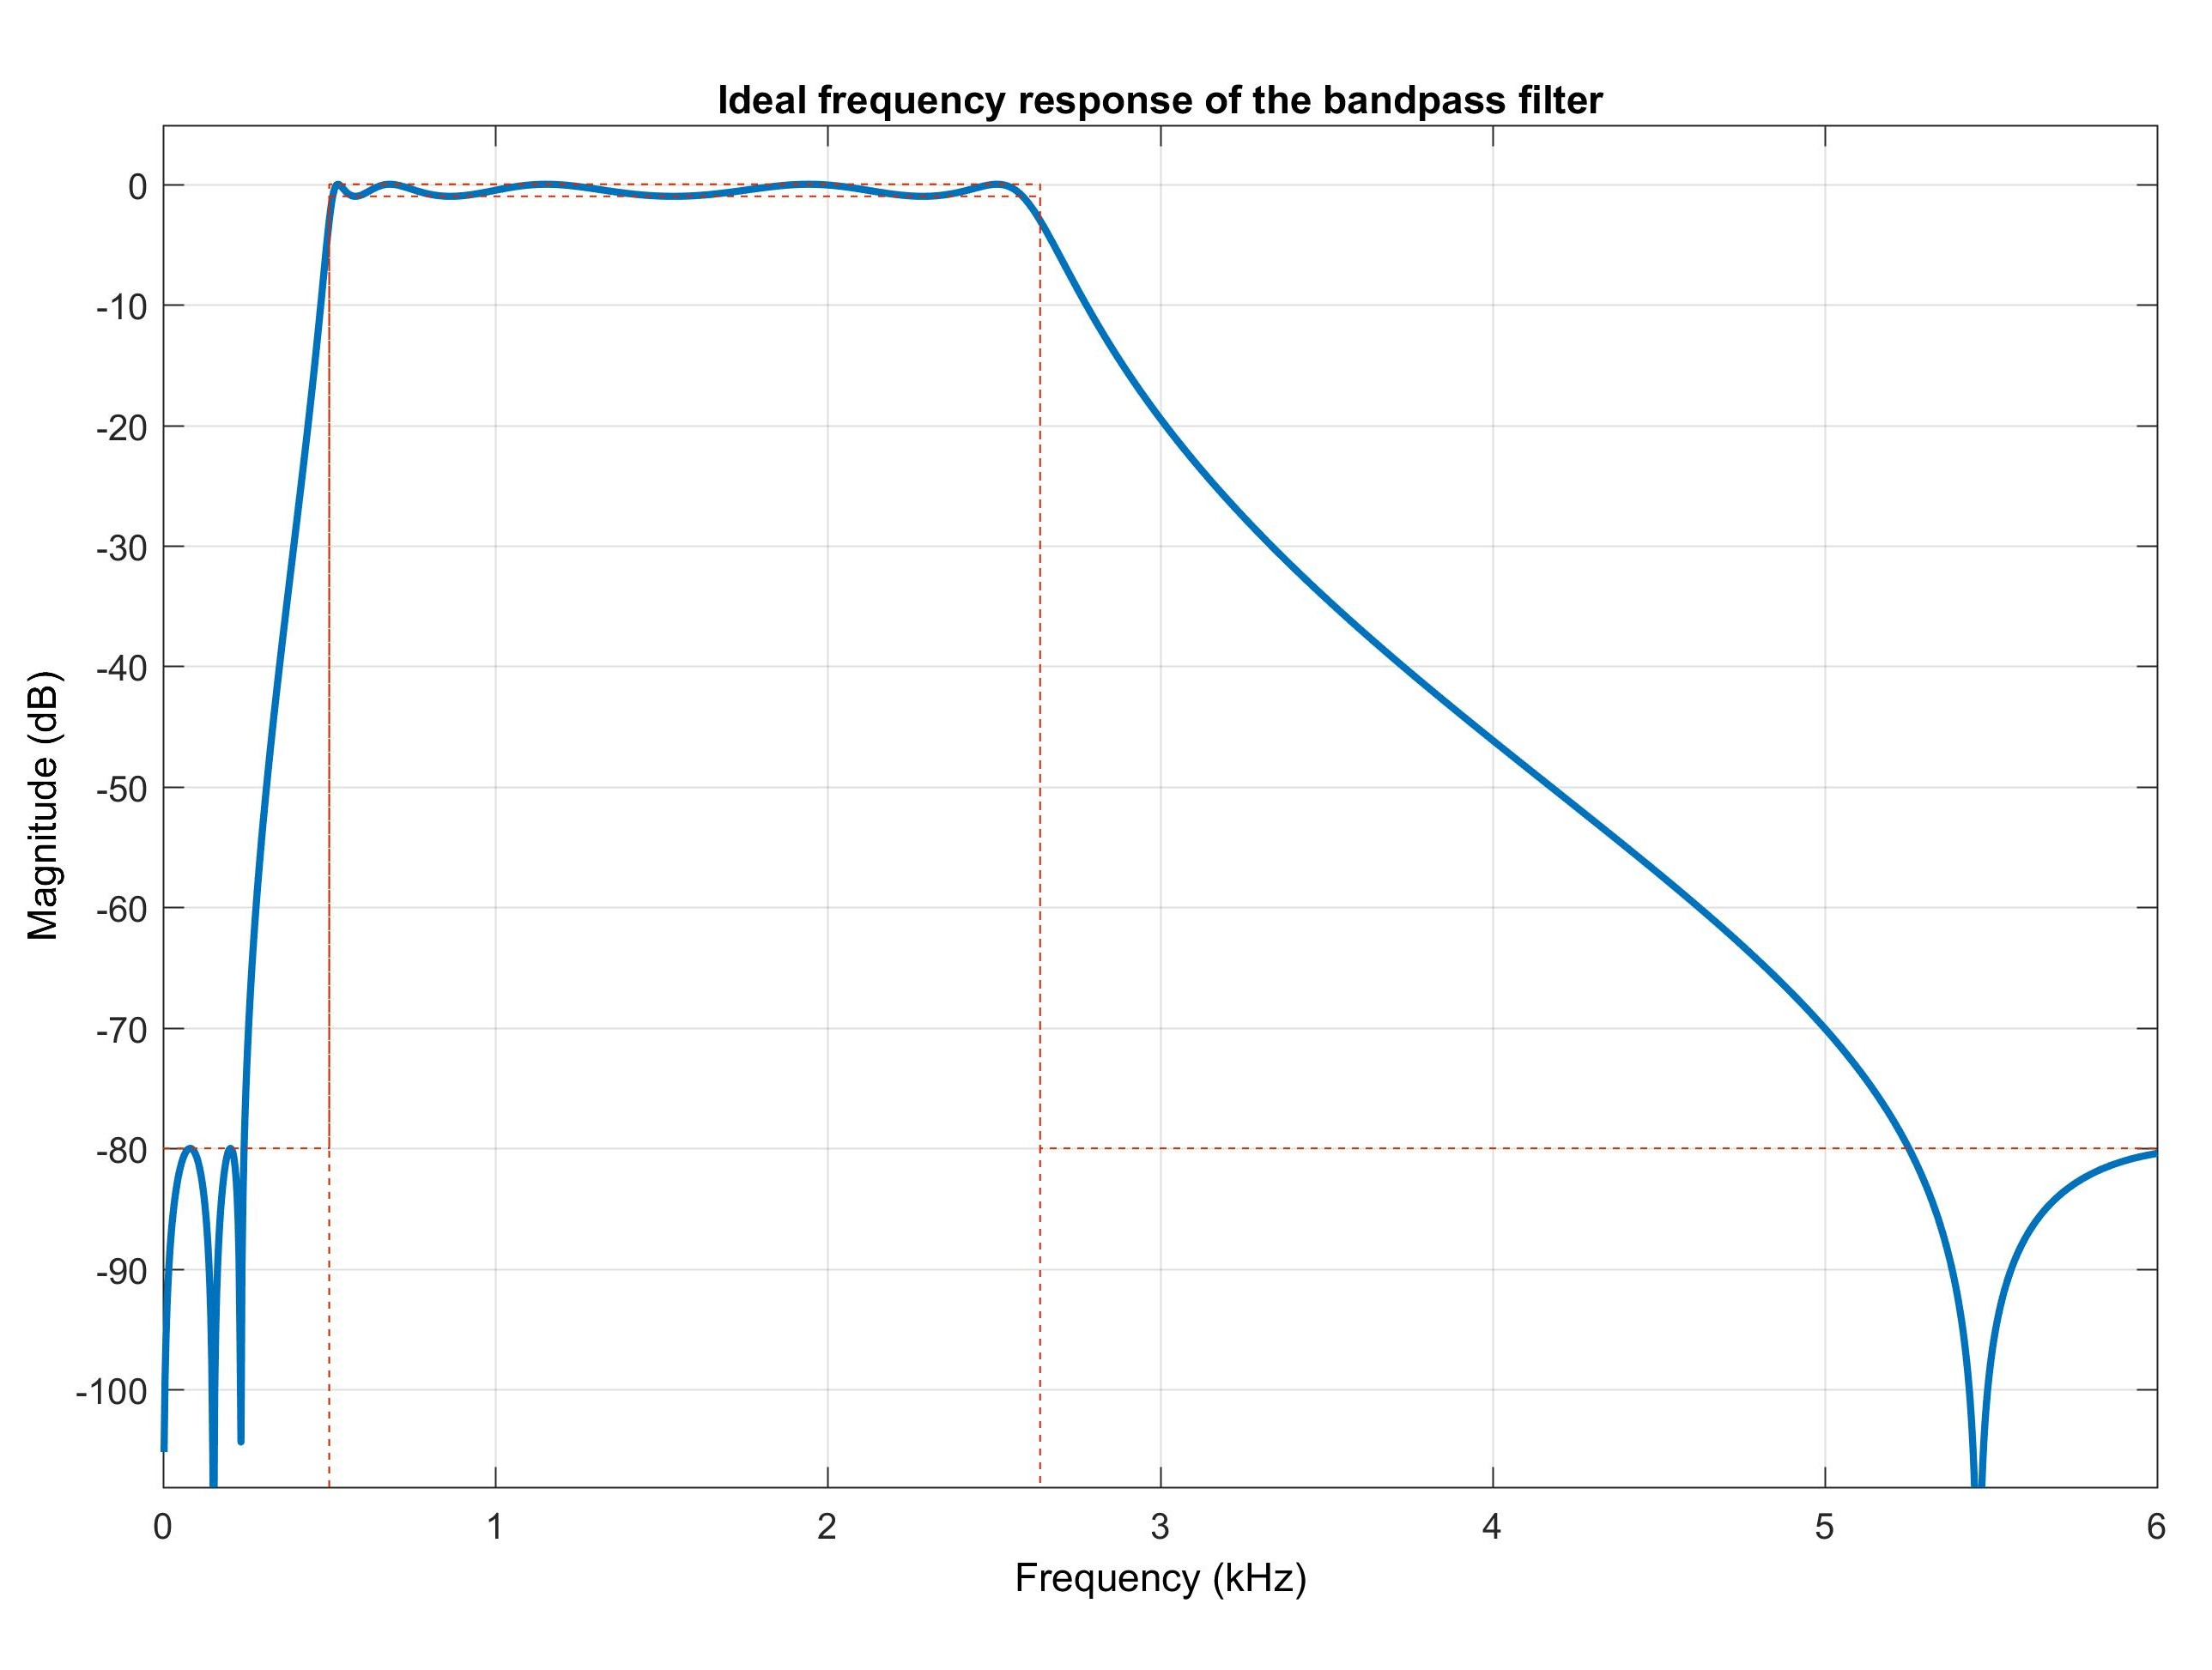
\includegraphics[width=14cm,height=14cm,keepaspectratio]{Figures/noise_bandpass}
\decoRule
\caption[Signal bandpass filter]{Bandpass filter of the test signal.}
\label{fig:noise_bandpass}
\end{figure}

The lower end of the filter is set to $500$Hz, which should generate $\tld 6\%$ of harmonic distortion at $-20$ of relative volume (table \ref{tab:relativescale}), rapidly decreasing at higher frequencies, this means the system behaves in a relatively linear way and the contrast figure doesn't suffer much from the distortions given by the higher harmonics.
\\
The figure below presents two graphs, the first one shows the frequency response of the estimated room transfer function in the bright zone, convolved with both the filter and the bandpass signal, as it will be outputted by the \textbf{first} speaker (number 15). As it can be seen, the power is concentrated in the $[500-\tld2200]$Hz range. Once the gains of the amplifiers will be applied to the signal in figure and the remaining seven loudspeakers (not shown) and outputted, we will record a \textit{linear combination} of such signals. The frequency response of the system (with all the 8 loudspeakers playing), as recorded by microphone 20, is presented in the second graph.

\begin{figure}[H]
\centering
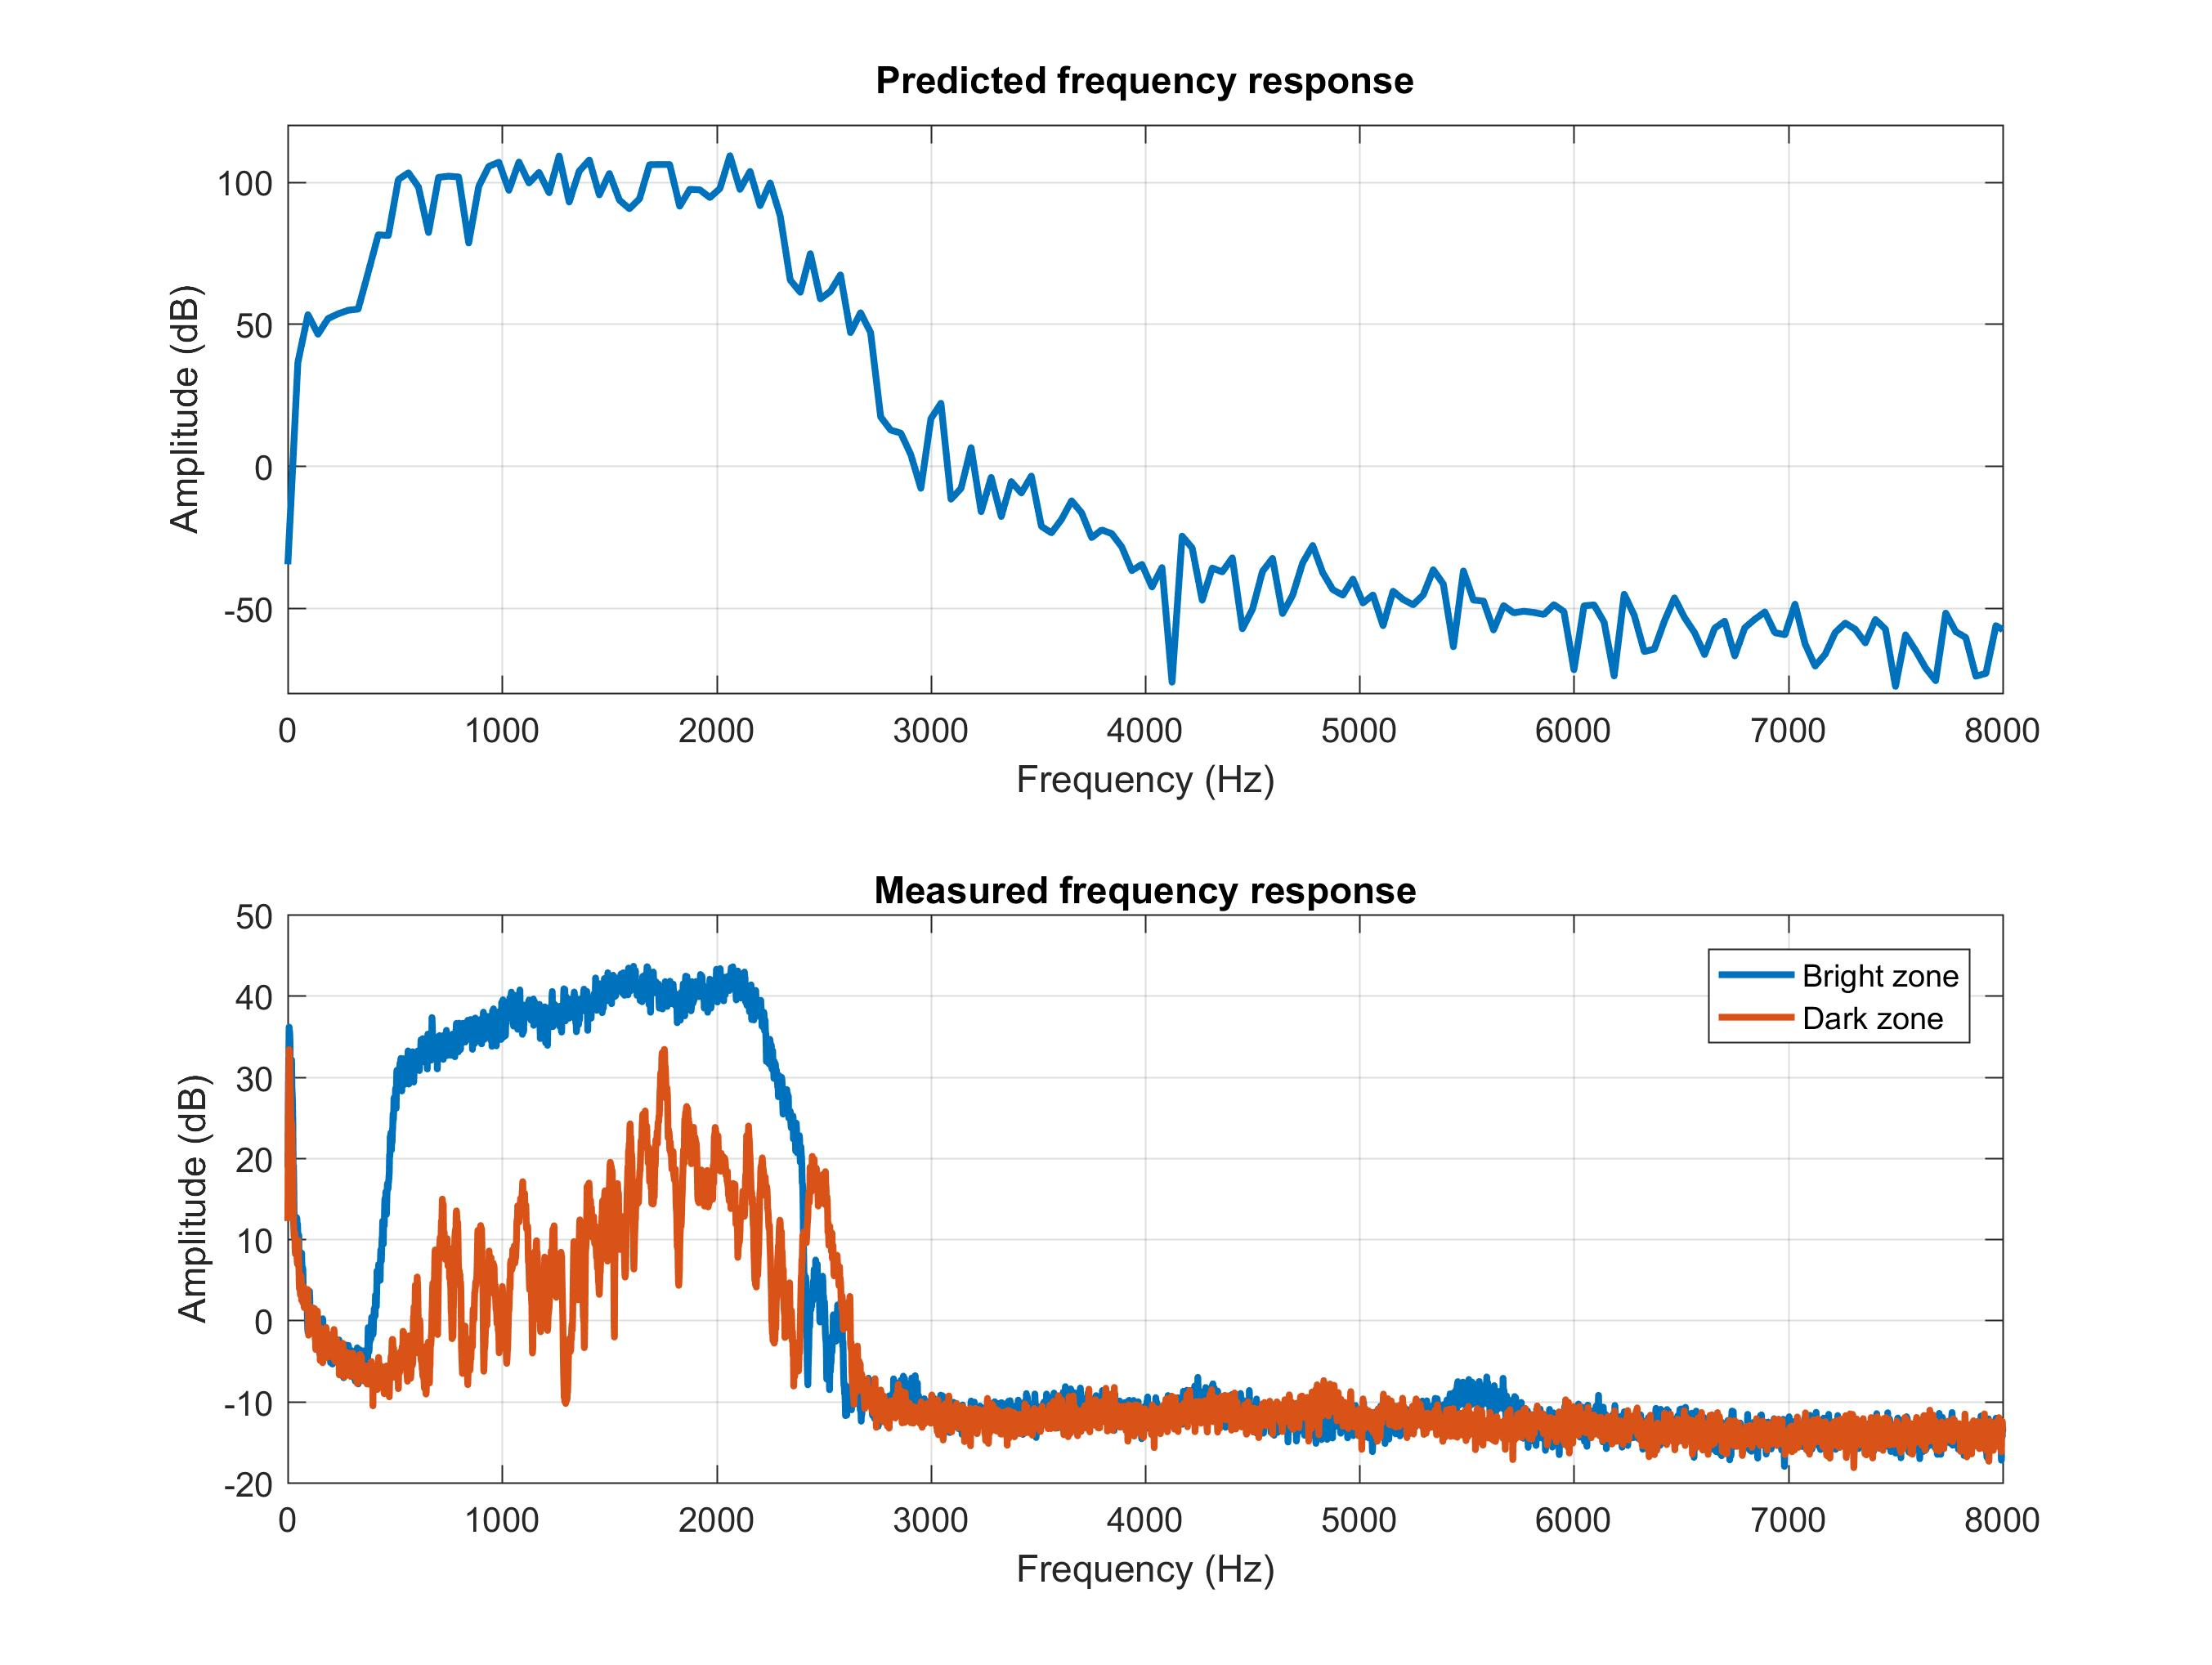
\includegraphics[width=15cm,height=15cm,keepaspectratio]{Figures/fftbacc}
\decoRule
\caption[Frequency response]{Predicted frequency response of the system when considering only the first speaker (first graph) and actual frequency response estimation of the system (linear combination of all eight speakers). Derived using the samples from microphone 20. The estimation was made by using the Fast Fourier Transform.}
\label{fig:fr_multiple}
\end{figure}

The blue line in the second graph represents the frequency content that is found in the bright zone. Please note that the graph is break down by frequencies, this means that the total energy in the zone is the sum of all the contributions from the single frequencies. The orange line in the same graph represents the frequency response of the system in the dark zone.
\\
\\
To get the resulting contrast we applied $10$s of bandpassed white noise, convolved with the BACC filter and recorded the result with four microphones ($20, 21, 28, 29$). These are the innermost microphones, inscribed in an imaginary square centered to the center of the matrix (figure \ref{fig:mics}). We haven't used all the $48$ units because of the increasing size of correlation matrices that this would have meant. As already explained, increasing this size means slower calculations. Using another set of microphones other than the innermost (for instance the outermost) would have changed the spatial aliasing frequency, since the distance between the control points would have increased.
\\
The final band of the system is $[500-\tld 2200]$Hz (an additional 9.1\% away from the Nyquist frequency has been left as bandguard). As previously stated, the signal, in order to be played, had to be upsampled to $48$kHz.
\\
\\
Looking at the second graph, we can see some unexpected behavior from the system. It appears to be some near-DC component in the spectrum, it might be some numerical error generated by the FFT function used, as it doesn't appear to be any low frequency noise when standing at the control point.
\\
The other unforeseen characteristic is that there is a small bias going towards the $2$kHz (and generally the higher) frequencies, the response in the controlled range is flat, in the sense that can be fit in a straight line with little defiation from it, but the \tld$10$dB slope going to the right of the frequency axis was not expected. The algorithm seems to "prefer" the higher frequencies, perhaps because they require less effort to be controlled. This behavior is seen even more prominently when decreasing the value of $\beta$ feed to the algorithm, since $\beta$ is a term that, applied to $RD$ (in equation \ref{eqn:lagrange}) penalizes the control effort.
\\
\\
The acoustic contrast is achieved by comparing the sound pressure levels of the same microphones in the two zones, said microphones have been previously calibrated by using a tone at $1$kHz at a known amplitude.
\\
With the regularization terms $\beta = 0.5$ and $\delta = 10^{-6}$, an output level of $-35$ relative scale (for each speaker) and doing an average of the four microphones used for the measurements, the volume of the noise in the bright zone is $\tld 70.1$dB, while the one in the dark zone is $\tld 45.5$dB. This value appears to be slightly lower than the one presented in table \ref{tab:relativescale} ($4.5$dB less).
\\
This can be attributed to the different kind of signal being outputted (bandpassed white noise, convolved with the BACC filter), rather than the Logsweep chirp.
\\
\\
This leads to a contrast figure of $\tld 24.5$dB, a value close to the theoretical result given by using equation \ref{eqn:contrast}. This is essentially in line with the results of \parencite{cai_time-domain_2014}, done with the same regularization parameters and in a similar frequency range (They present $\tld 27$dB of contrast in a range of $[200-1900]$Hz). Once again, the reader might wonder about the reproducibility of the results. Running the algorithm five times seems to lead to an uncertainty of $\pm 2$dB. I want to stress that affirming this cannot substitute a statistical analysis, which is done with hundreds (or thousands) of data samples. It is encouraging though that the uncertainty seems to be somewhat bounded and in line with the results of the simulated environment. The fact that the time interval used is $10$s gives some robustness against statistical outliers in the noise, hence normalizing the contrast figure.

\subsection{Analysis of the Bacc-RD method using different filter lengths and regularization terms}{}
\label{subsec:baccvary}

Now that we have tested the effectiveness of the algorithm with some real setup we can start asking ourselves some new questions: how do the regularization terms affect the contrast figure?
\\
Similarly, how is the frequency response in the bright zone affected by them? 
\\
How much does the length of the IR affect the performance of the filter?
\\
\\
In order to answer to all of these questions we have to generate a considerable amount of filters obtained using different parameters and test them in sequence inside the anechoic chamber.
\\
The parameters we are going to evaluate are (equation \ref{eqn:lagrange}):
\begin{enumerate}
\item The IR length $I$. The values tested are: $200, 300, 400, 500, 600$.
\item The control effort term $\beta$, with values equal to: $0.1, 0.5$.
\item The regularization term $\delta$, we will choose: $1\text{x}10^{-2}, 1\text{x}10^{-6}$.
\end{enumerate}
The total number of filters tested is $80$, each one of these has been applied twice. The following graphs gives an insight on how do these terms affect the contrast figure.
 
\begin{figure}[H]
\centering
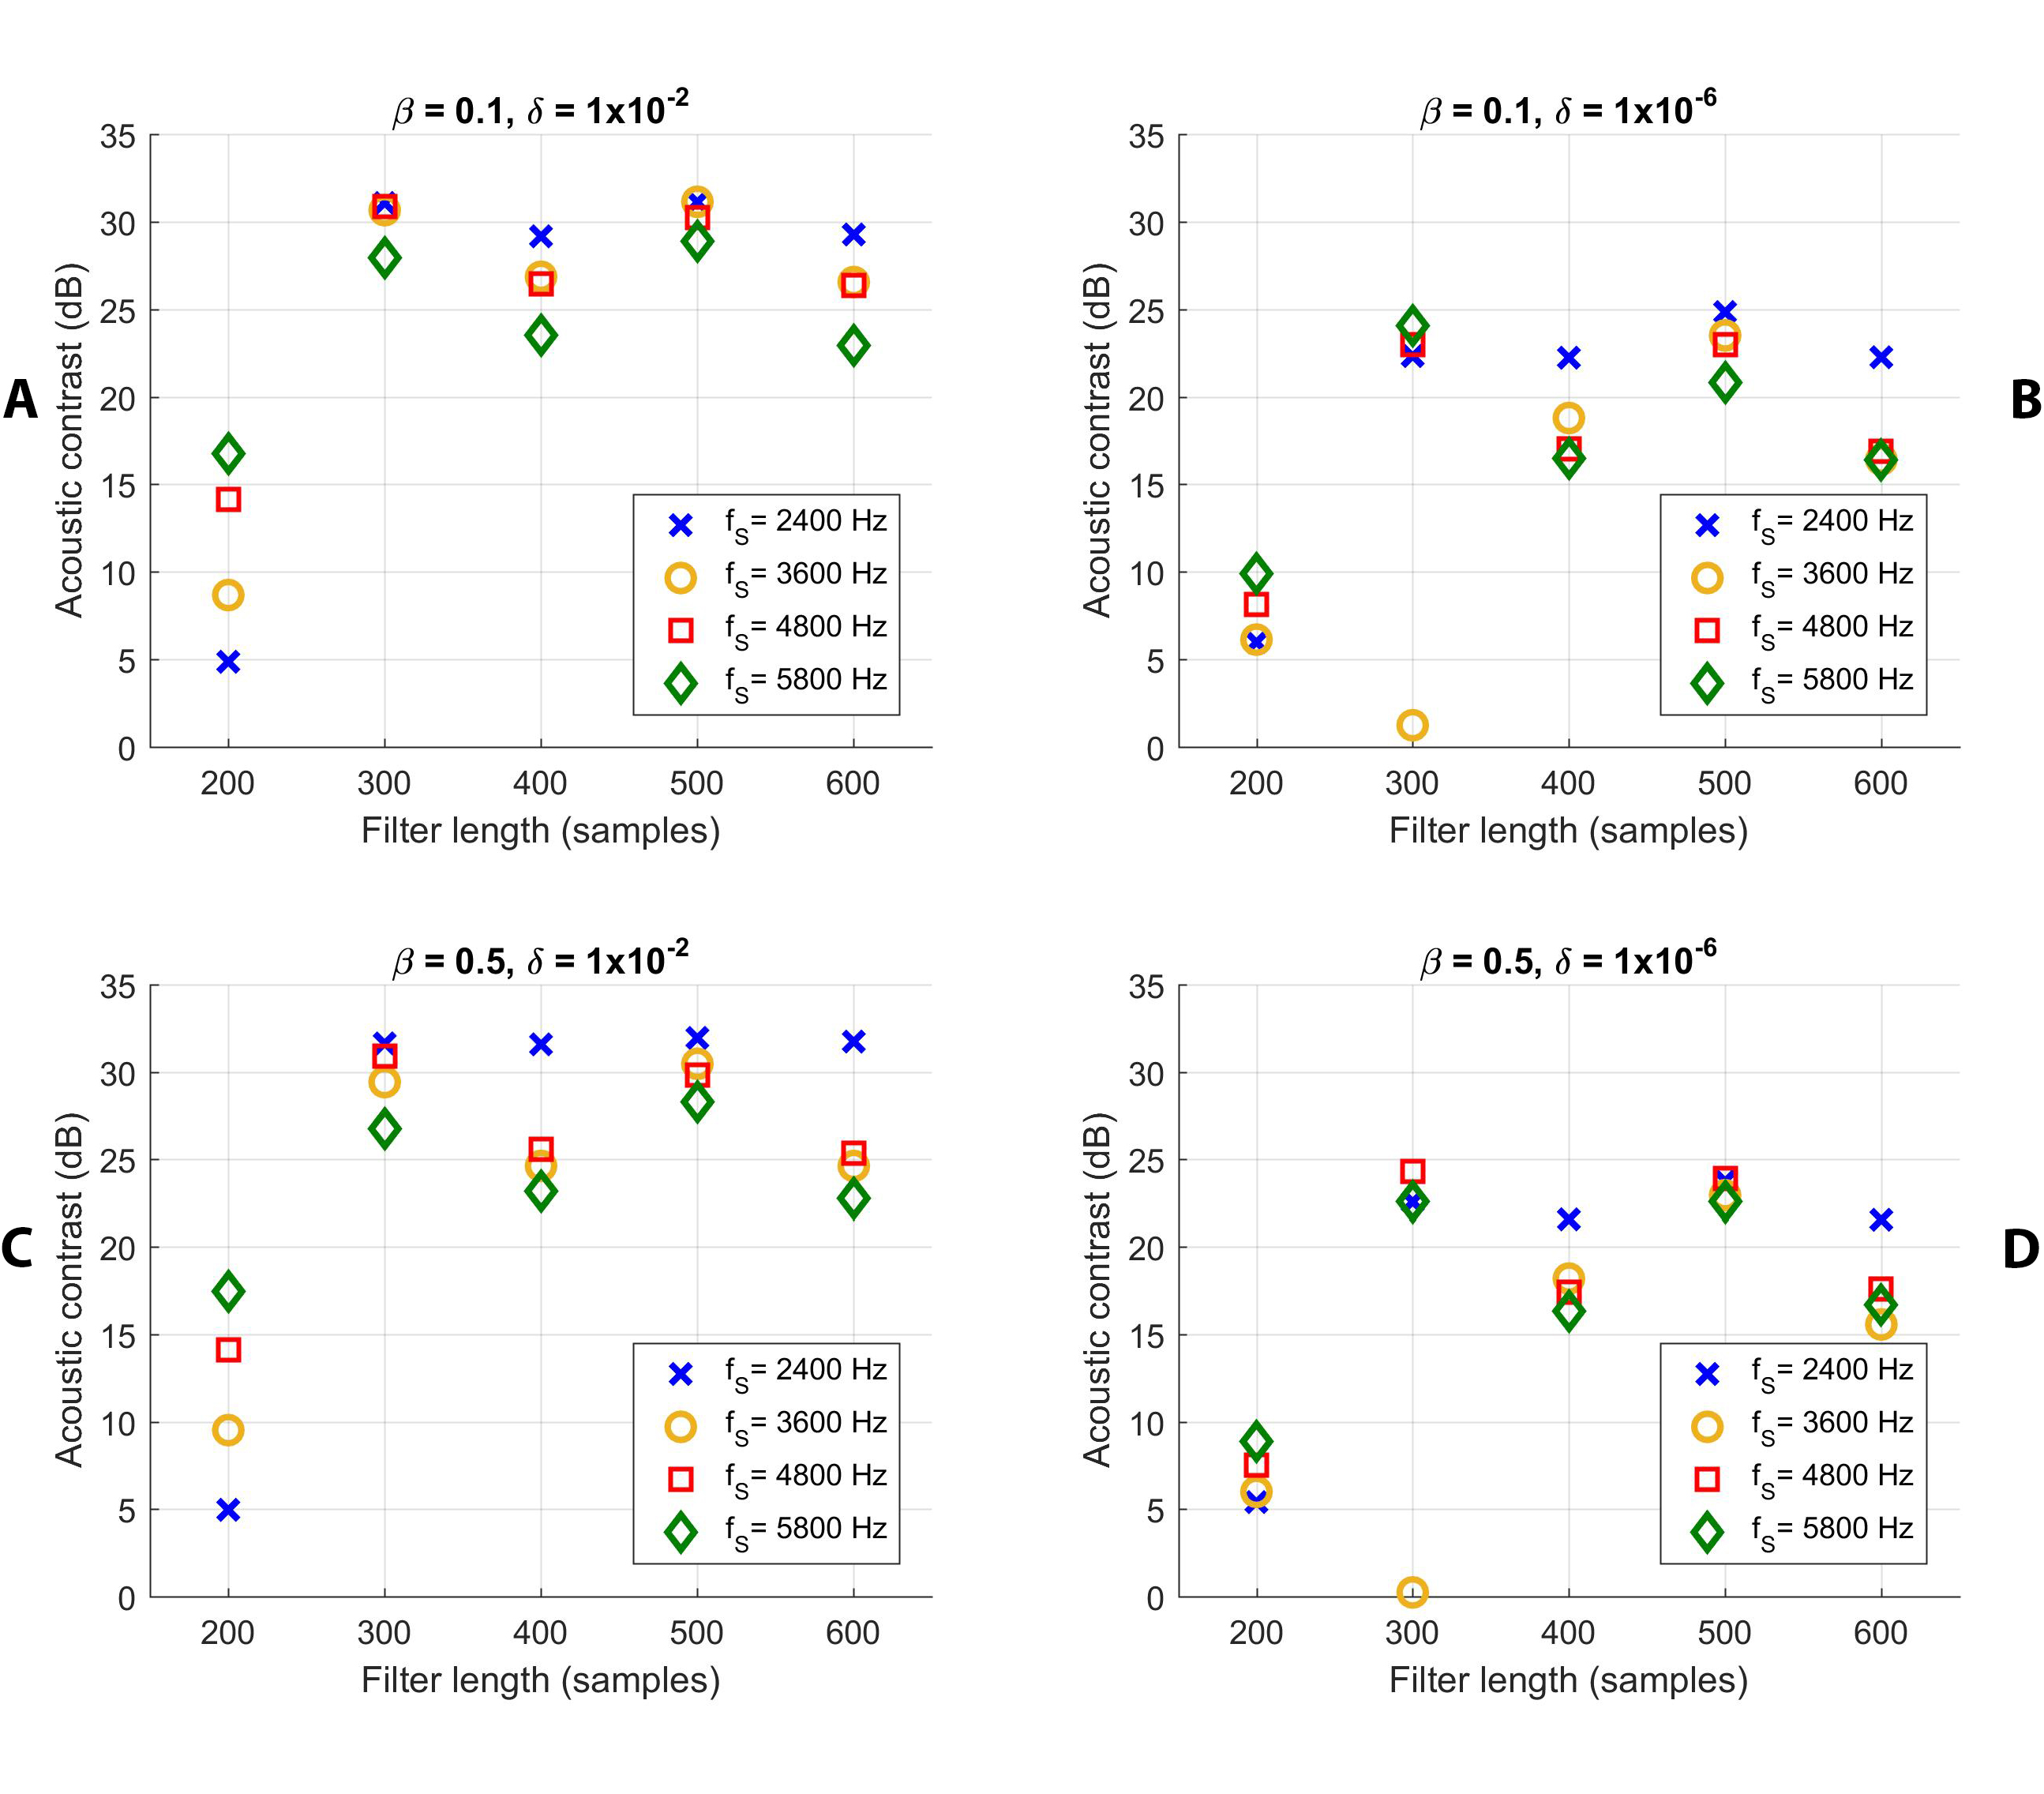
\includegraphics[width=15cm,height=22cm,keepaspectratio]{Figures/comparison_COMP}
\decoRule
\caption[Comprehensive comparison of the filters]{Comparison of 80 filters varying sampling frequency, $\beta, \delta$, filter length.}
\label{fig:comparison1}
\end{figure}

The above figure presents all the $80$ filters used, divided in four categories of $20$, depending on the values of $\beta, \delta$. The four symbols represent the different sampling frequencies used when testing the weights vector calculated using equation \ref{eqn:optimization}. Like the experiments performed in section \ref{subsec:baccrdanechoic}, the original signal, having a sampling frequency of $48$kHz, is downsampled to the value listed as $f_s$ and the upper frequency limit of the test signal is adjusted accordingly. Specifically, the sampling rate is slightly more than double $f_{UP}$, the upper frequency limit, which is determined by the Nyquist theorem, minus a \tld$9\%$ of band guard. The lower frequency bound is still $500$Hz for all of the signals.
\\
The sampling frequencies $f_s$ used are $2400, 3600, 4800, 5800$Hz, while the upper bounds $f_{UP}$ are \tld$1100, 1650, 2200, 2650$Hz, respectively. 
\\
\\
Looking at the figure we can see some patterns. At a length of ($200$samples) for the IR (and the BACC filter, since they are set to have the same value) we see that we have little contrast. This is due to the fact that we are losing too much informations regarding the system by choosing a value that is too small. In fact, if we look at figure \ref{fig:ir_bright}, we see that we have NO information about the system itself, but only some artifacts introduced by the Logsweep signal.In fact, it is very surprising to see that we have some contrast at all. Upon further investigation we can see that the contrast figure itself is artificial. By looking at the filter weights we discover that some loudspeakers are set to play at a louder SPL than others by the algorithm

\begin{figure}[H]
\centering
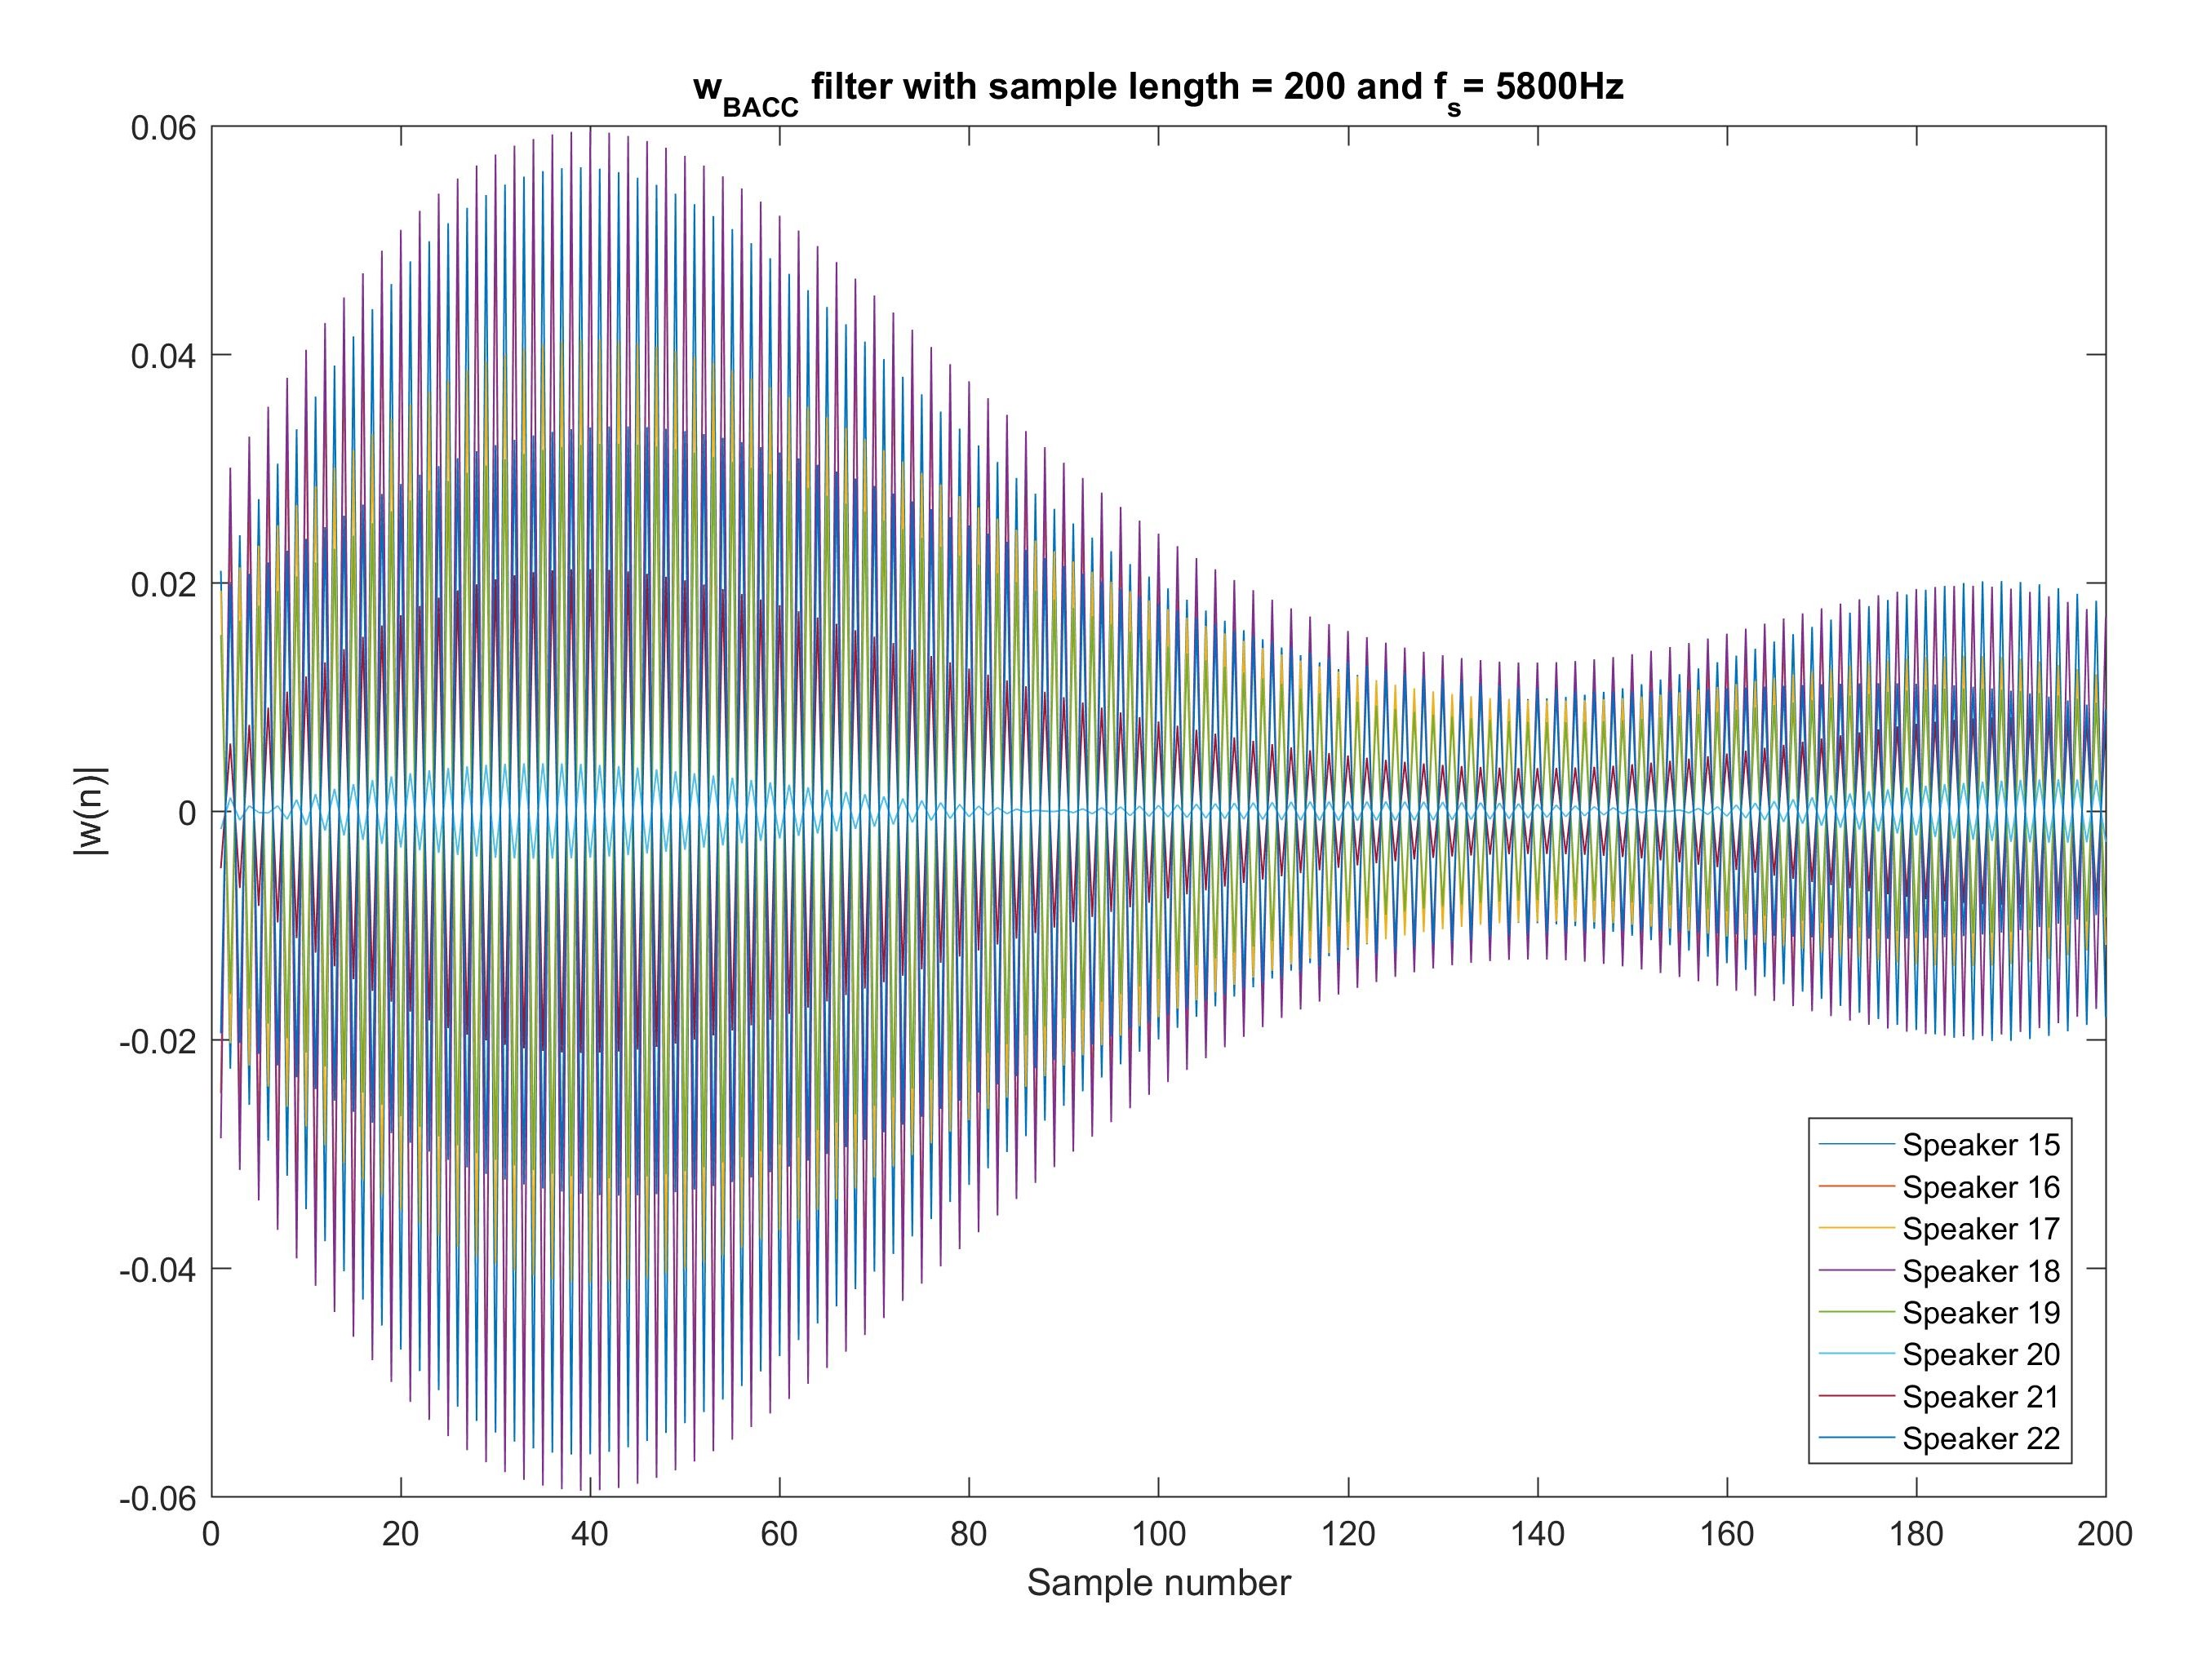
\includegraphics[width=15cm,height=15cm,keepaspectratio]{Figures/filter_strange}
\decoRule
\caption[Superimposed amplitude]{Superimposed amplitude of the BACC filter for all the eight loudspeakers}
\label{fig:filter_strange}
\end{figure}

From the figure it appears that the shape of the weights of the various loudspeakers is similar for all of them, this demonstrates that those filter have been calculated with no actual information content about the system other than the distance between loudspeakers and zones. This is derived indirectly by the samples in the IR that show the artifact coming from the estimation method (Logsweep). The only parameter that changes is the amplitude of the weights, this means that the filter simply increases the sound pressure generated by the driver closer to the bright zone, while the ones adjacent to the dark one are quieter. This difference in SPL is therefore given just by the different propagation of the sound in the room, and it's not the result of destructive interference.
\\
\\
This behavior shows a limitation of the algorithm, the fact that we have no penalization on the control effort, in other words the loudspeakers can be played at whatever volume. To solve this problem it appears necessary to introduce a new constraint on the maximum output allowed to each unit, trying to match all the individual pressure levels. If this technique was to be implemented, the contrast figure when the filter length is too short for the system in question should be (ideally) zero.
\\
\\
Moving away from the edge case and extending the IR length to at least $300$ samples, allows us to design some filters that can contrast sound. We see that lower $f_s$ not only have the highest performances, but also have the best stability in the contrast figure achieved (A, B, C, D). This is because the low sampling frequency (and the smaller frequency band of the test signal) eliminate part of the oscillations of the IR, lowering the overall resolution of the  estimation, having more delay between samples also means that the IR represents a longer time span of the system, giving a more complete characterization. Conversely, even though higher sampling frequencies have a better time resolution, the wider band they use introduces more variance (C), which means that the realization of the noise $\textbf{E}\{AWGN\}$ can alter the results in a more decisive way.
\\
From the graph above we can also see the influence the two parameters $\beta, \delta$ have in the contrast. Comparing (A, C) and (B, D) it appears that $\beta$ has little effect on the contrast itself. This is to be expected, since, as previously explained, $\beta$ controls the "shape" of the frequency response of the system

\begin{figure}[H]
\centering
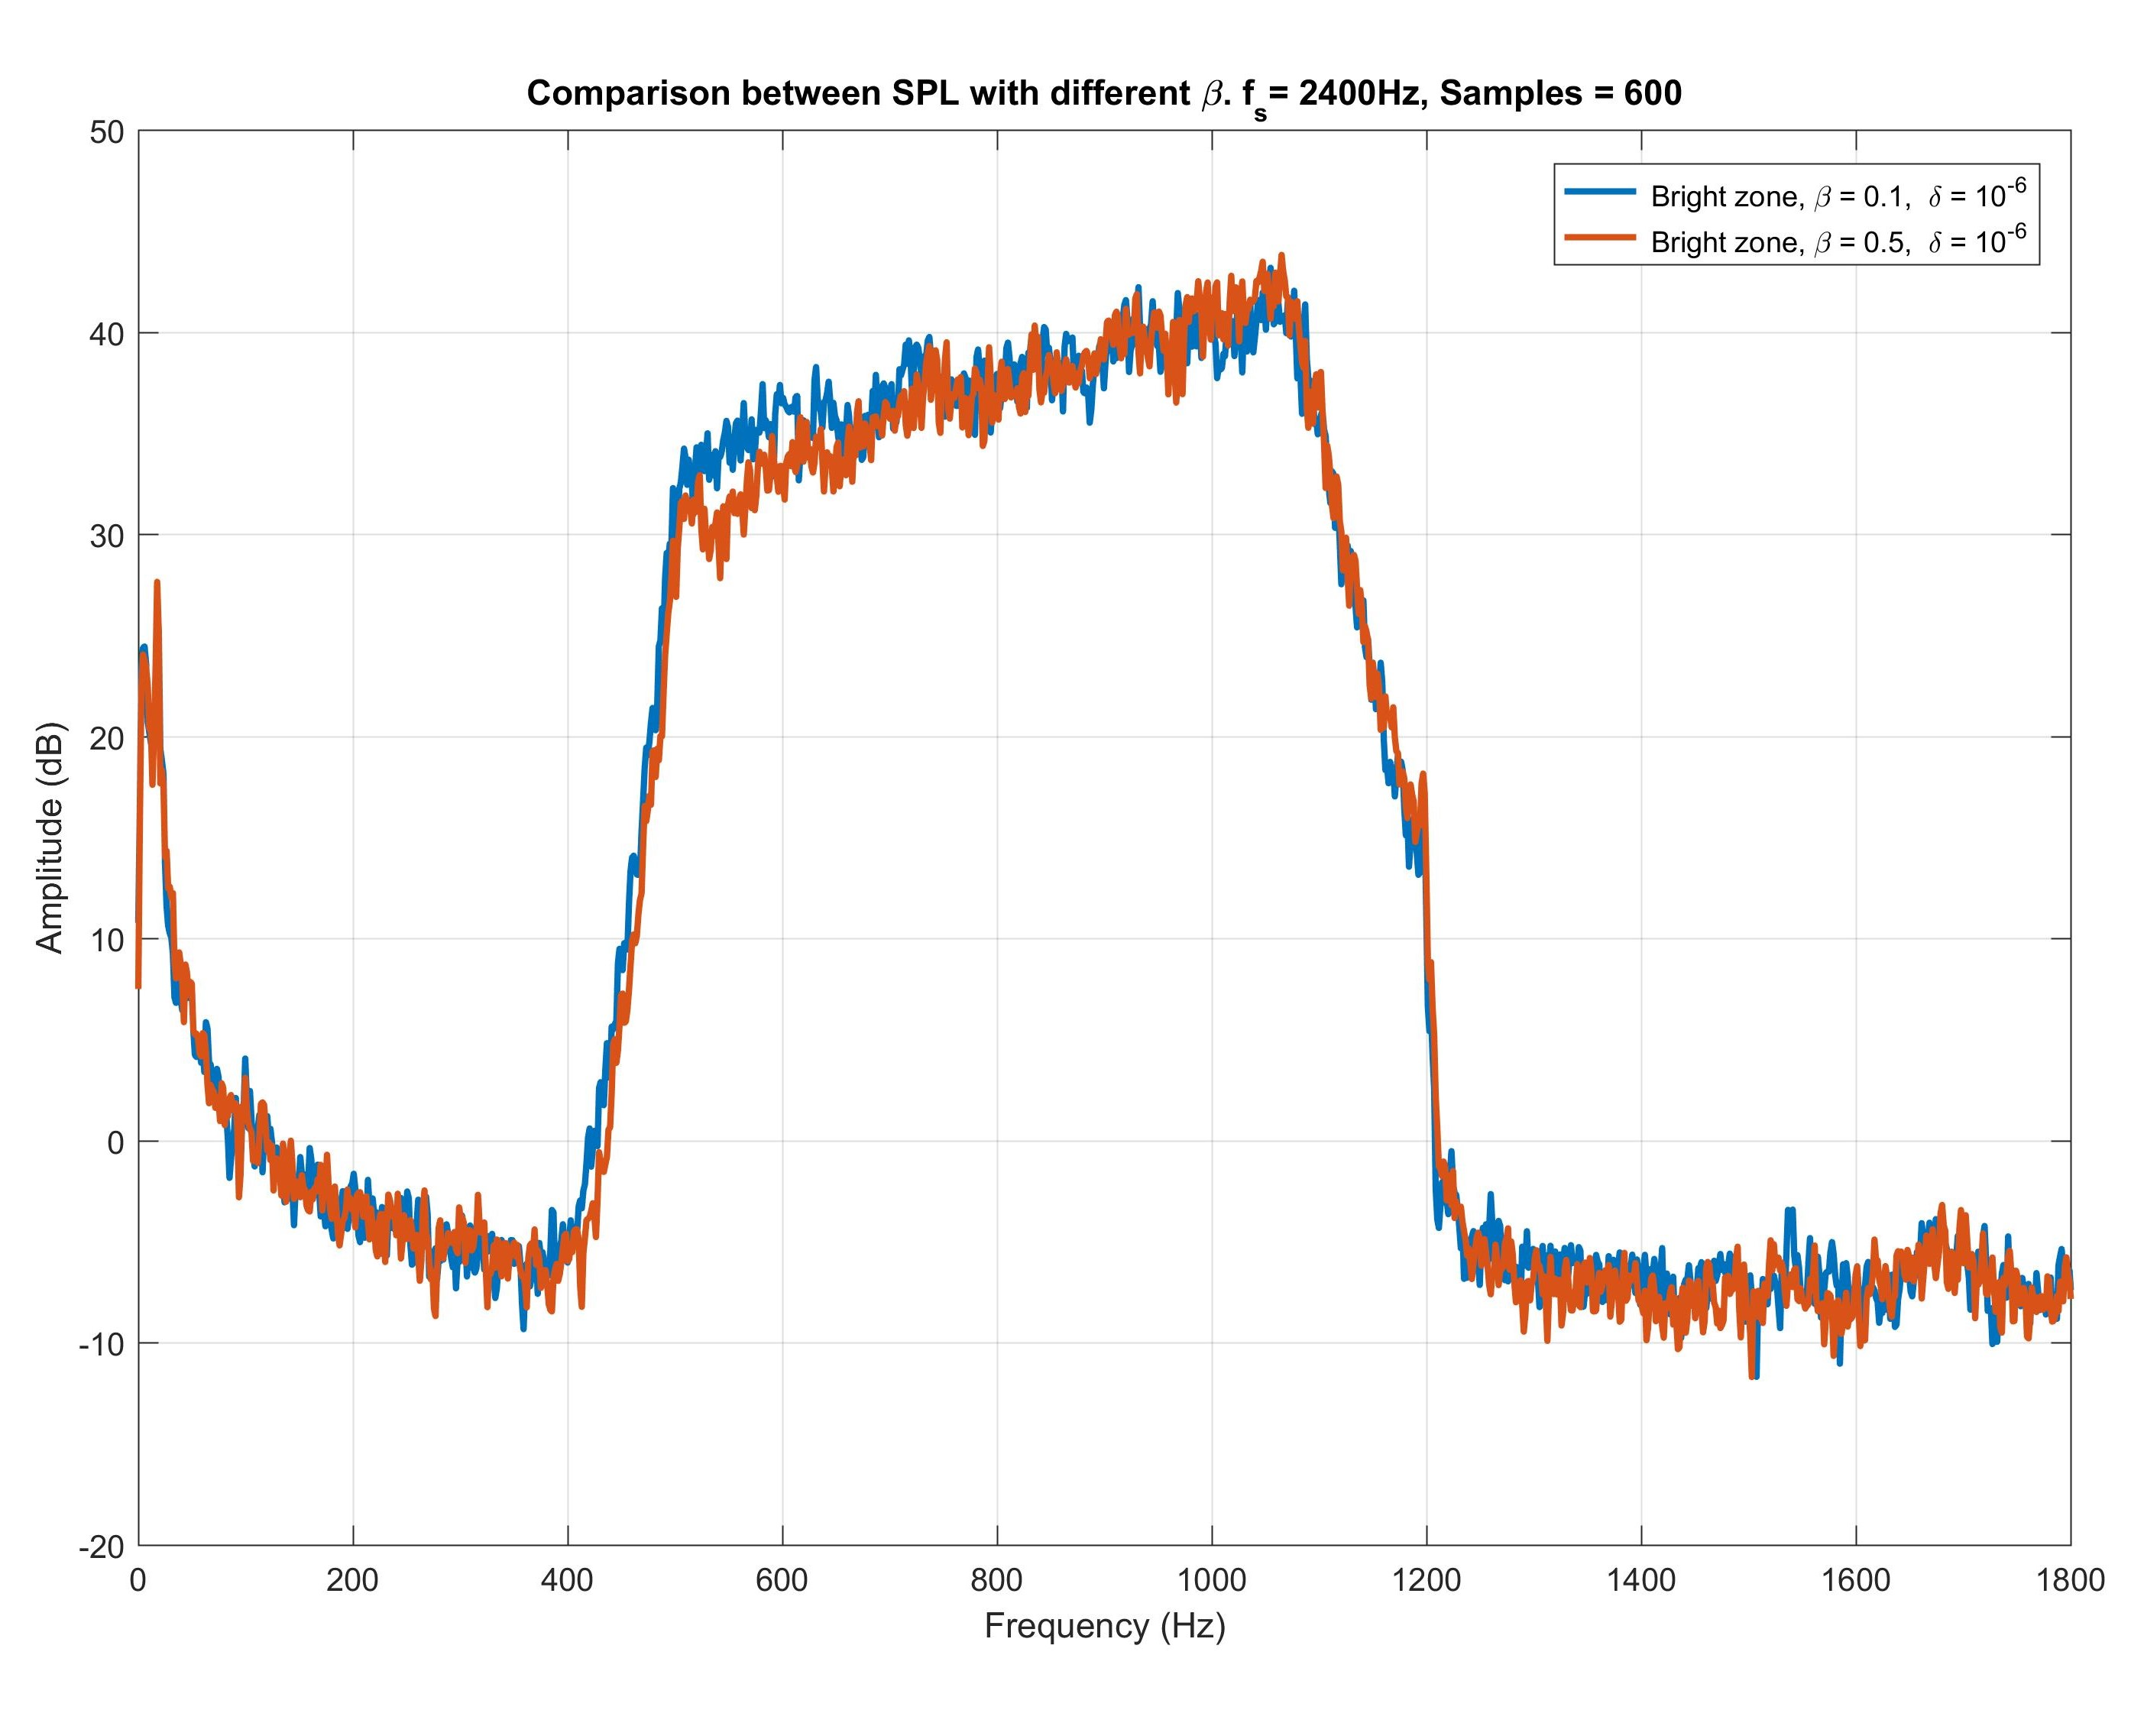
\includegraphics[width=14.5cm,height=15cm,keepaspectratio]{Figures/filter_25vs65}
\decoRule
\caption[FFT filters same delta]{FFT of the recording of microphone 20 for two filters with different $\beta$.}
\label{fig:filter_25vs65}
\end{figure}

The figure shows the Fourier Transform of two filter (both with $f_s = 2400$Hz and $600$ samples) as recorded by microphone 20, positioned in the bright zone (graphs B and D). We can see that the frequency response of the system is very similar in both cases, and in general not affected by $\beta$. What is effected instead is the slope of the frequency response in the range of interest, this is because a lower value of $\beta$ penalizes less the alteration of the shape of the FR, so the algorithm tends to maximize contrast in the higher part of the spectrum, therefore by skewing the response. The contrast figure of the two filter is $22.2\pm2$dB for the first one (blue line) and $21.8\pm2$dB for the second (orange line).
\\
\\
The value of $\delta$ instead affects the contrast figure as shown in graphs (A, B) and (C, D). This is because $\delta$ determines the error bound, the maximum deviation an element of the correlation matrices $R_b, R_d$ is allowed to have before being discarded for the calculation of the maximum eigenvalue in equation \ref{eqn:lagrange}. A lower bound implies an higher sensitivity of the algorithm. 

\begin{figure}[H]
\centering
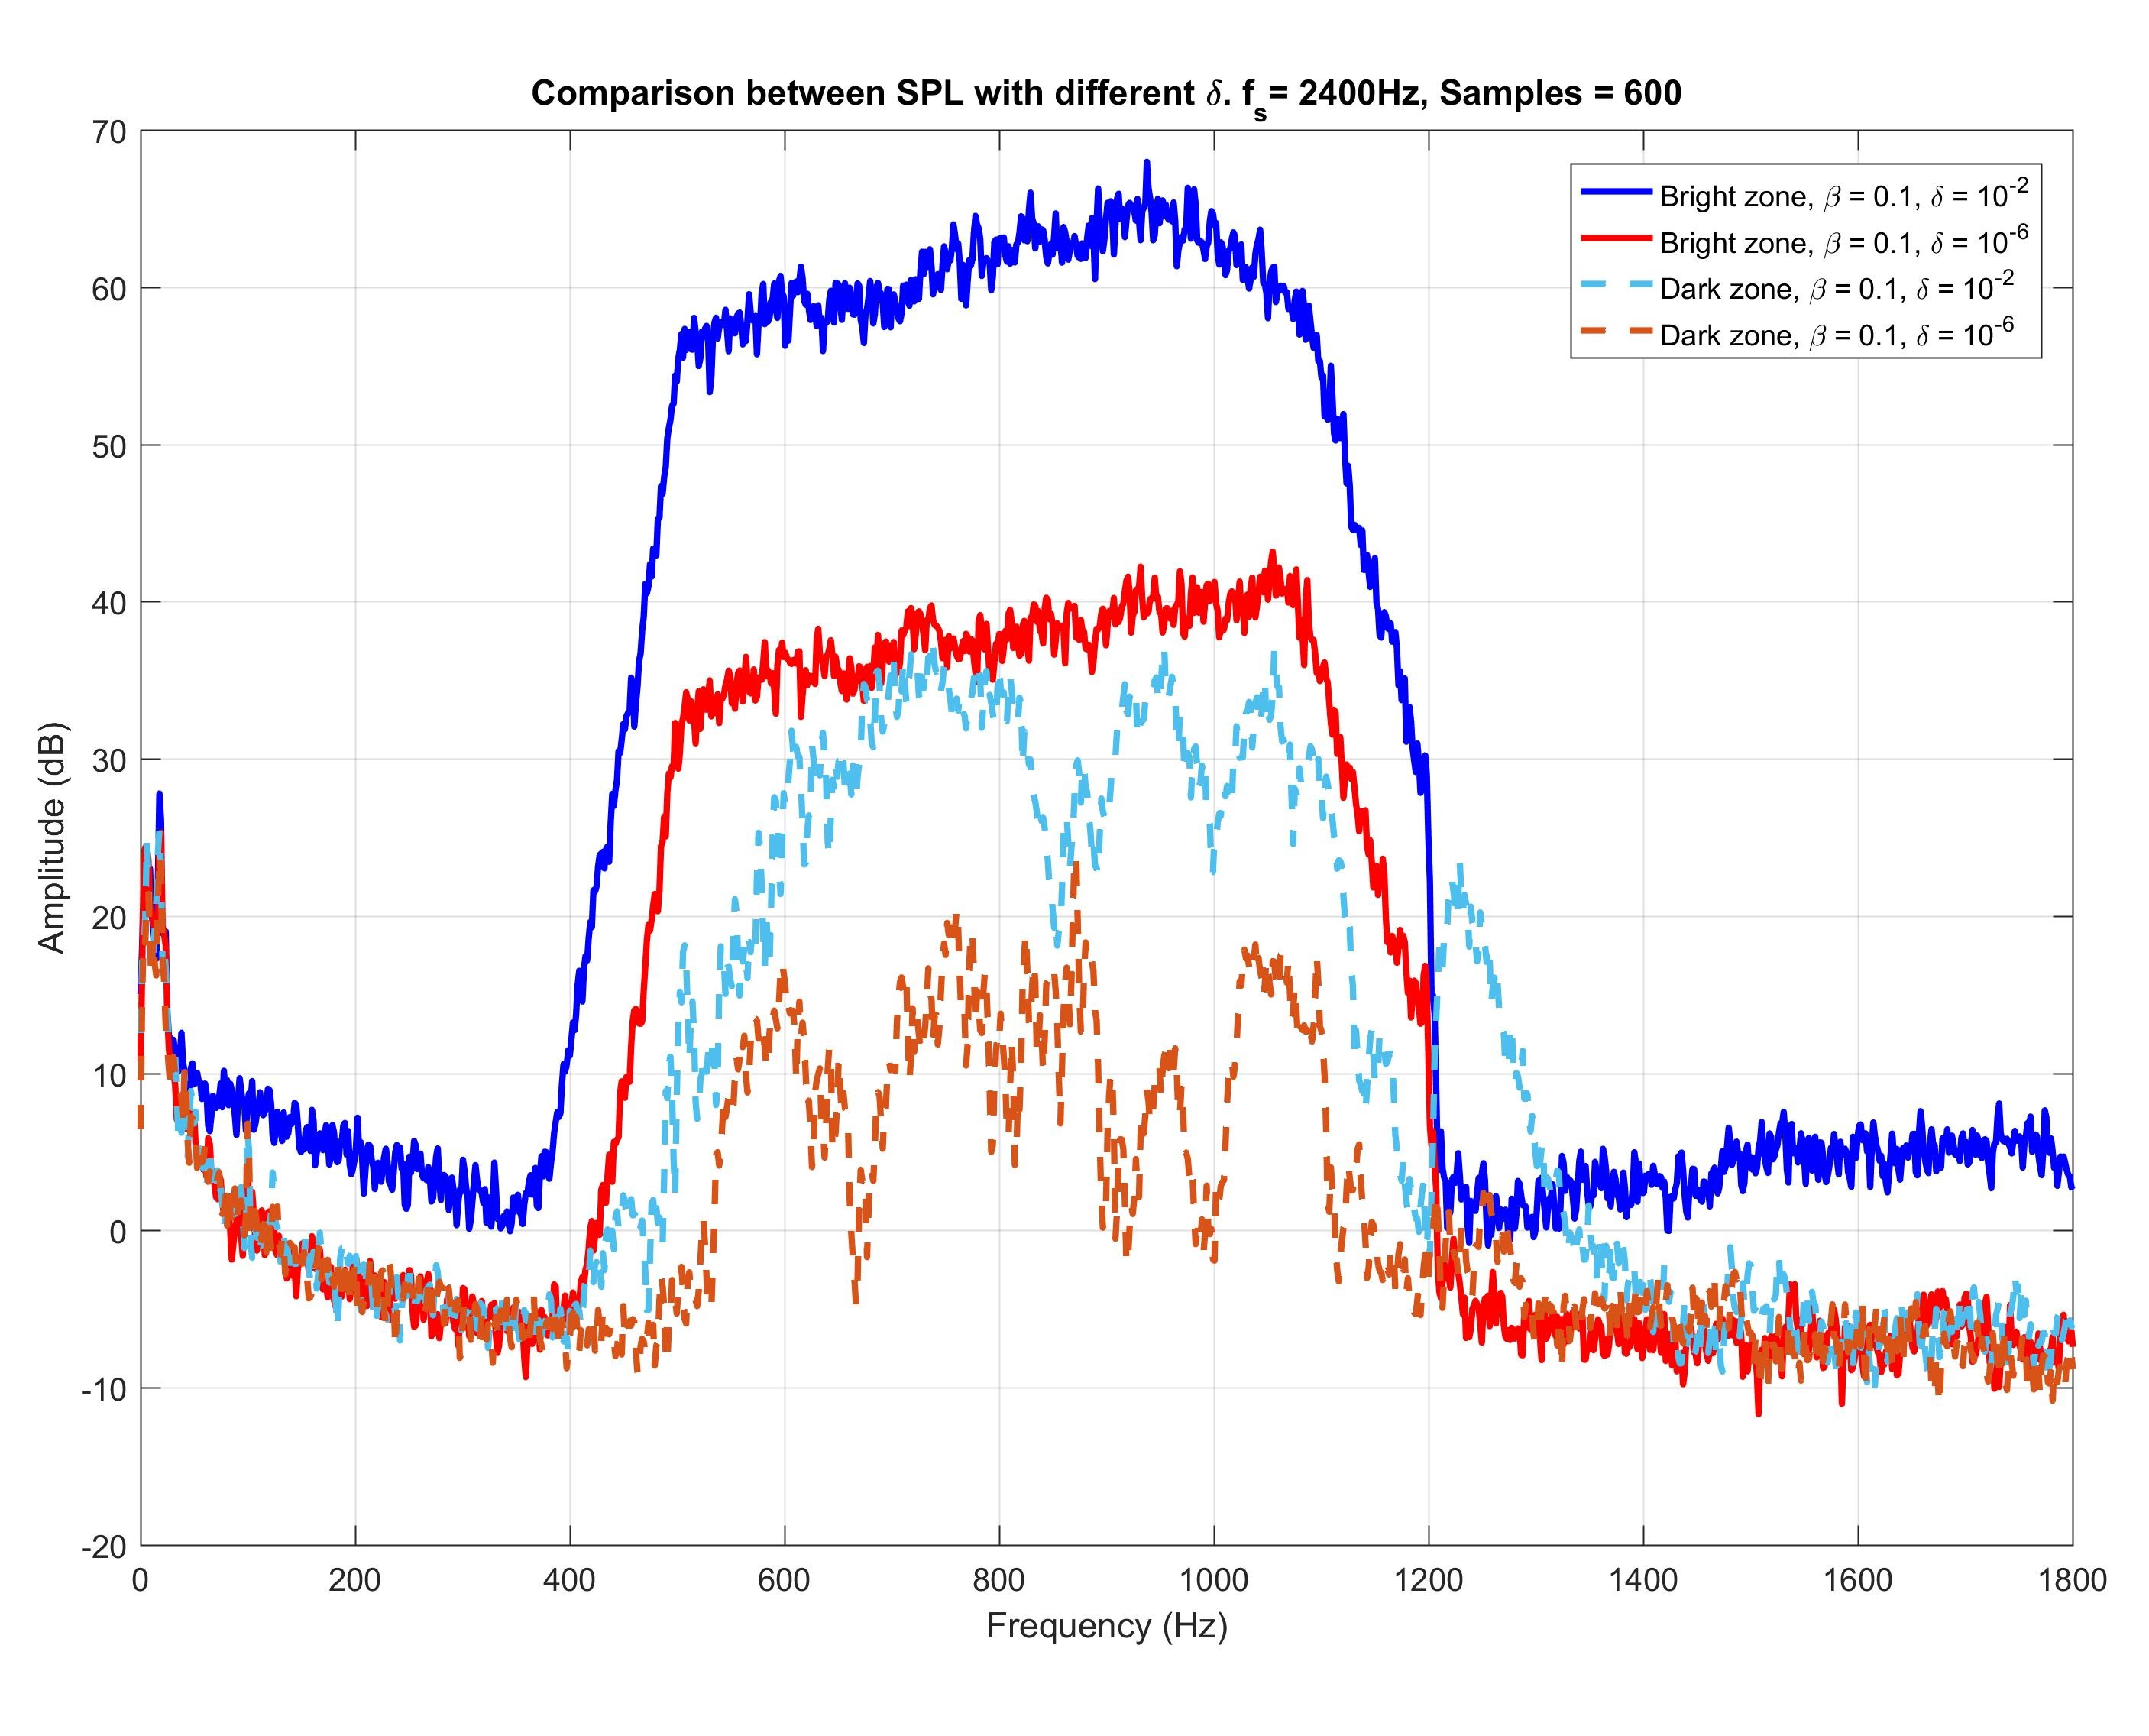
\includegraphics[width=14.5cm,height=15cm,keepaspectratio]{Figures/filter_5vs25}
\decoRule
\caption[FFT filters same beta]{FFT of the recording of microphone 20 for two filters with different $\delta$.}
\label{fig:filter_5vs25}
\end{figure}

As shown in the figure, even though a value of $\beta = 1\text{x}10^{-2}$ grants an higher contrast ($29.2\pm2$dB, blue vs light blue line) its behavior in the range of interest ([500-1100]Hz) is less linear compared with the filter which has $\beta = 1\text{x}10^{-6}$ ($22.2\pm2$dB, red vs light orange line), meaning that the variations of SPL with regard of frequency are less predictable and the mean square distance from its mean value is bigger.
\\
\\
In the end we can say that increasing the filter length over $300$ samples is not so important, since it appears that the algorithm does a good enough job with few samples, this is probably due to the "easy" test environment given by the anechoic chamber, which has a relatively short IR.

\subsection{Splitting the system Impulse Response}{}
\label{subsec:filtersplit}


We have looked at the algorithm and the effect that changing some parameters have. We will now add a reflection source in the anechoic chamber, such as the one described in section \ref{subsec:reflector} and draw some conclusions.
\\
The panel is situated at $1$m from the microphone matrix and $30$cm to the right from the center of the second speaker array, roughly behind the bright zone, the rest of the setup is identical as the one presented in figure \ref{fig:anechoicsetup}.
We can see what kind of effect such an object has, when estimating the system impulse response, by using the Logsweep method.

\begin{figure}[H]
\centering
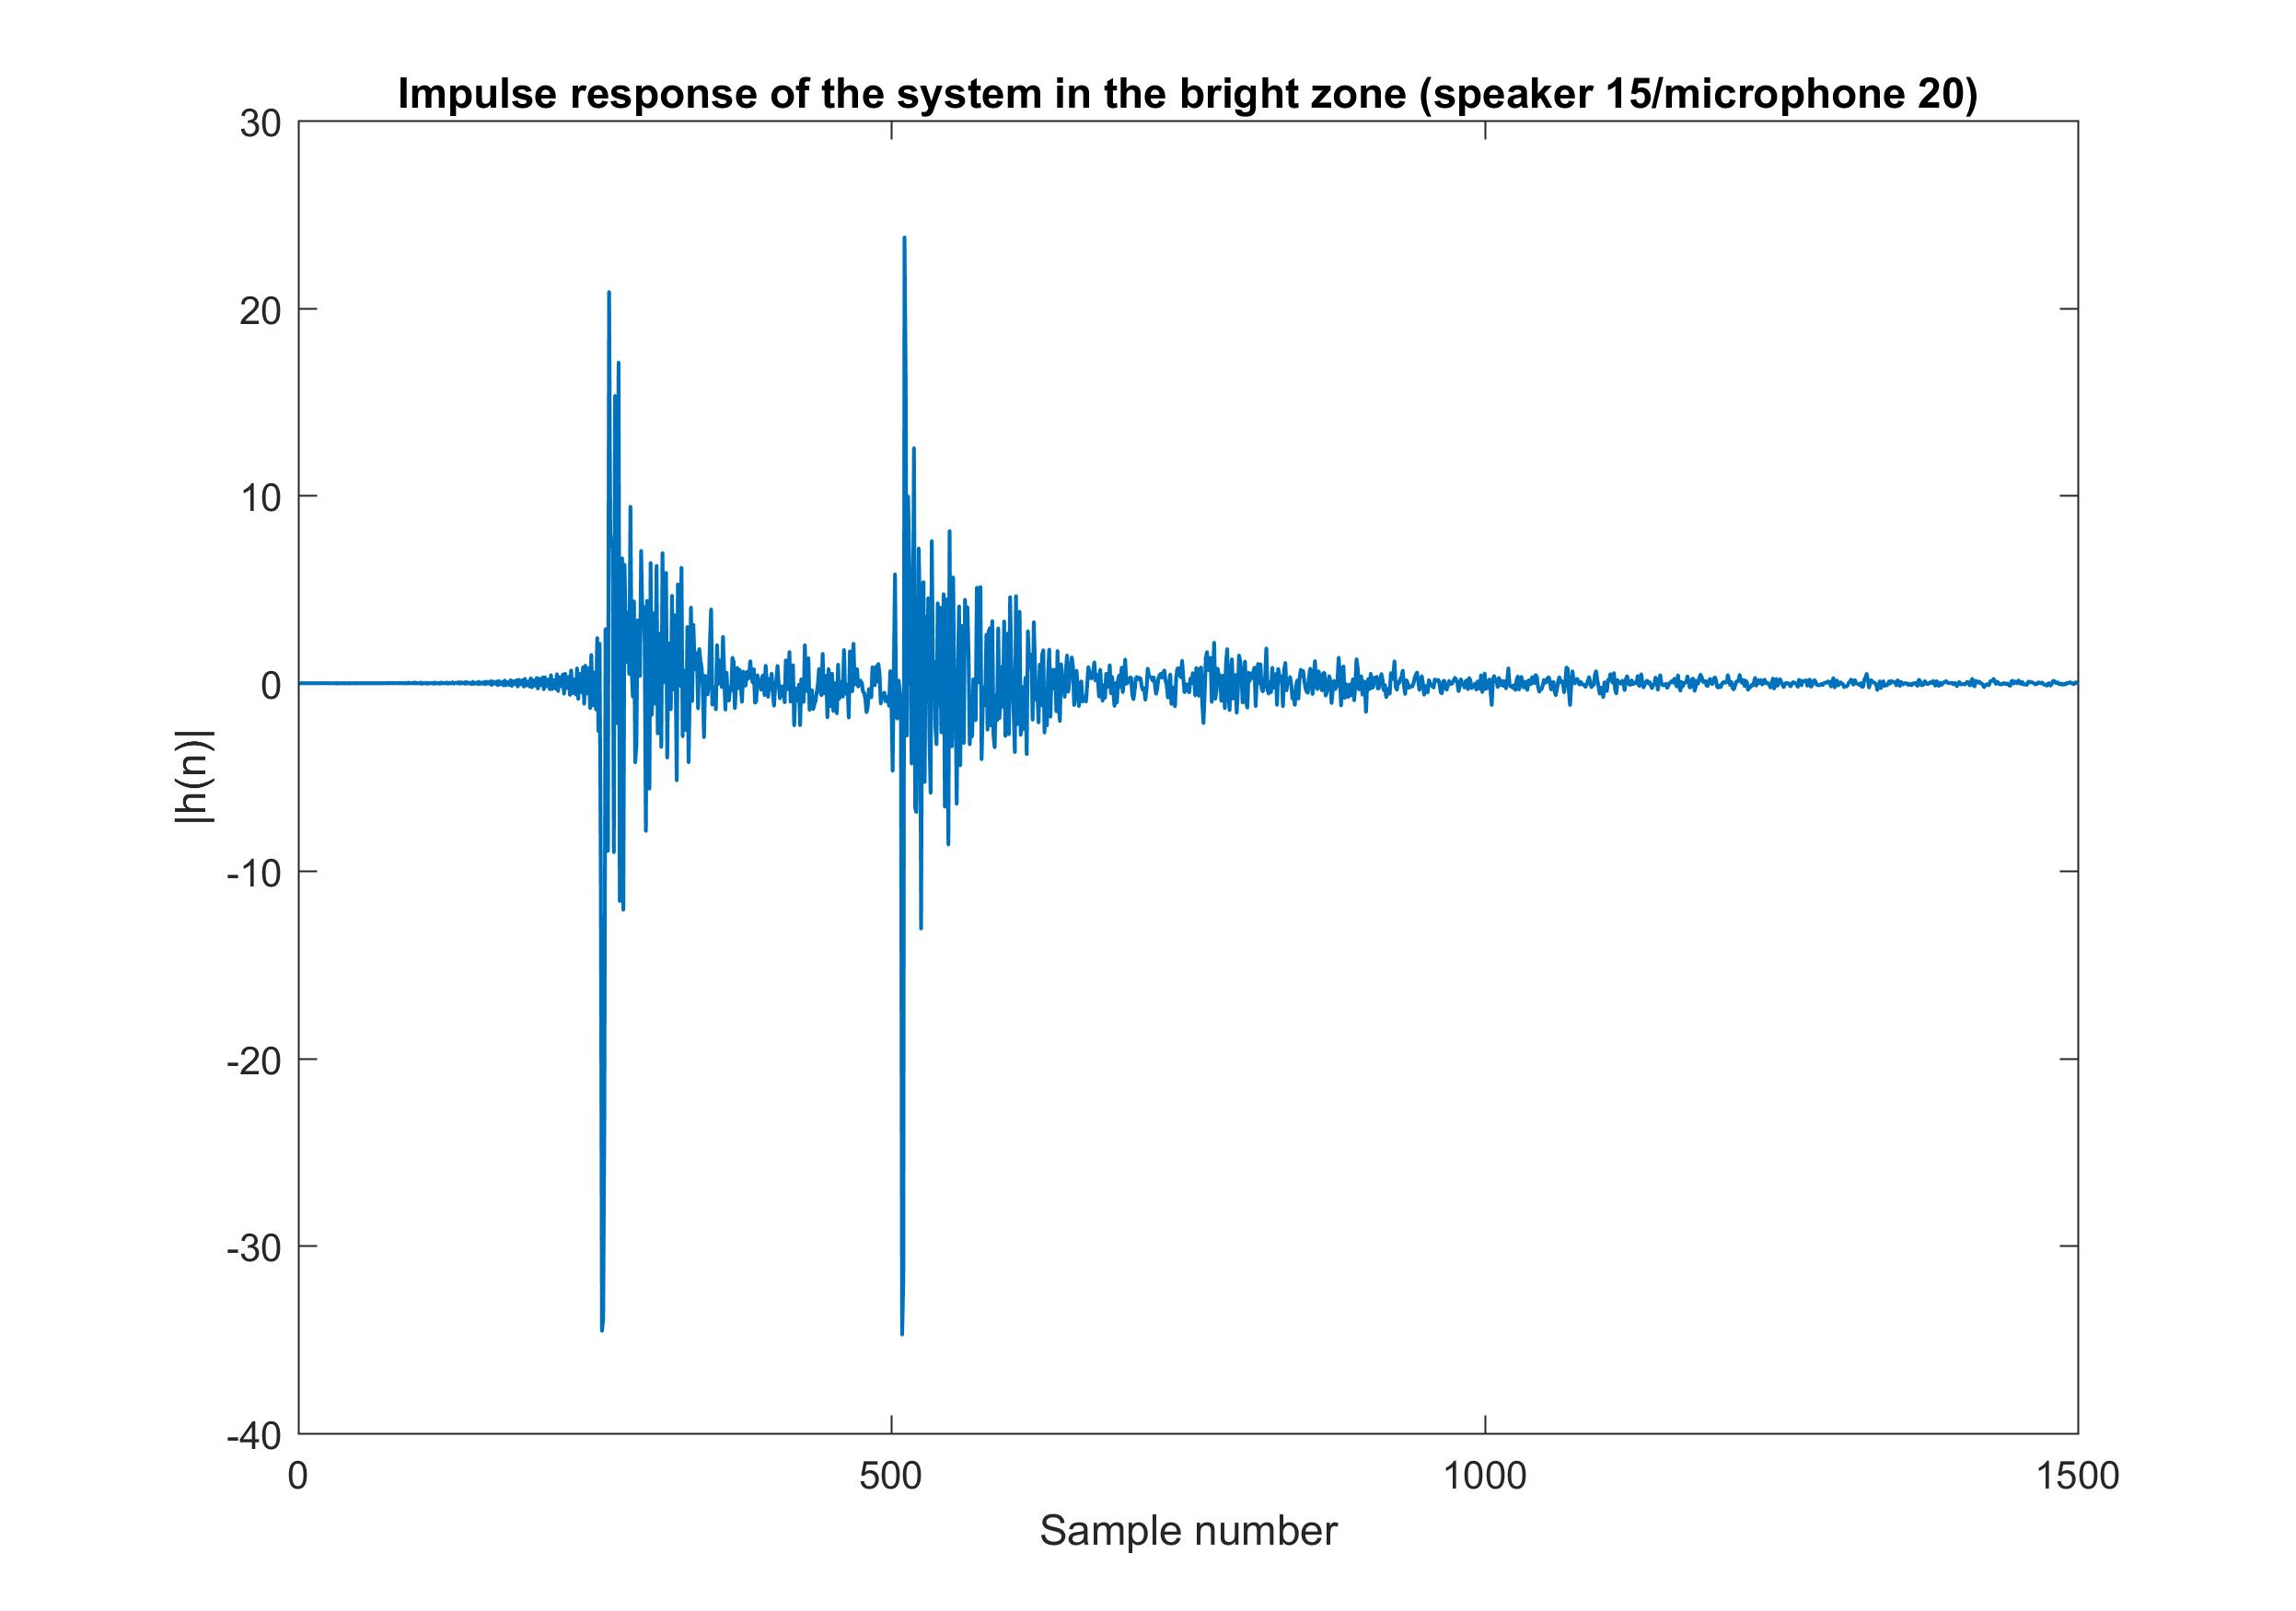
\includegraphics[width=15cm,height=15cm,keepaspectratio]{Figures/ir_refl_bright}
\decoRule
\caption[Impulse response]{Impulse response of the system.}
\label{fig:ir_refl_bright}
\end{figure}

The second peak from the left in the IR represents the soundwave being reflected by the panel and hitting the microphones, after it had passed them a first time (represented by the first peak, which corresponds to the hit of the direct wave). The reader can compare the IR presented above with the one in figure \ref{fig:ir_bright}.
\\
The distance between the two peaks is strongly tied with the position of the reflector, the more distant it is from the microphone matrix, the later (higher in sample number) the peak will appear. Moreover, we can notice a longer tail in the IR, this means that more samples (moving to the right of the graph) will now have some information content. In other words, we need more samples to represent the system with a relative accuracy and ignoring the long tail when running the ACC algorithm will lead to a decrease in the contrast figure.
\\
\\
Rerunning the experiment of section\label{subsec:baccrdanechoic} (the first one in the anechoic chamber, with the same parameters of $\beta=0.5$, $\delta=1\textbf{x}10^{-6}$, same filter and IR length $M=I=400$ and $-35$ of volume in relative scale), we can see the contrast figure be reduced to $20.6\pm2$dB (compared to $24.5\pm2$dB of the first experiment, the one without the reflector).
\\
This is because of two reasons. First and more importantly, the reflection source introduces more energy to the room, it redirects soundwaves that have already passed the control zones, back towards said areas, both for the controlled and the non-controlled (higher harmonics) frequencies. This is effectively increasing the amount of nonlinear distortions present in the soundzones at a given time, reducing the contrast.
\\
The second consequence having the surface in the room has, is to increase the length of the IR necessary to have a good estimation of the channel, as we can see from the longer tail from the graph above, cutting short the IR would lead to an unacceptable information loss. With a downsampling factor of $10$ and a filter length of $400$ samples (like the first experiment) the loss is still acceptable, so this effect is less noticeable, but if the source was to be positioned further back, or if we would have defined a shortened filter vector (maybe because we wanted to decrease the computational time), we would have incurred in noticeable worsening of the contrast figure.
\\
\\
The idea of shortening the filter length is particularly interesting, since the algorithm, as it stands, it's too heavy to run on any other machine other than high performance, multi-core CPUs and even in that case it requires minutes, if not hours, to come up with the correct weights vector that constitutes the solution to the Lagrange problem \ref{eqn:lagrange}.
\\
\\
Ideally, we would like to shorten the filter length, without compromising the contrast figure.
\\
The fundamental idea behind the solution for this problem is made possible by the fact that the filter length and the IR length are independent from each other. Instead of designing a long ACC filter for the system, we could find some parts, two in this case, where the IR has the most information content, those correspond to the samples in proximity of the two peaks. We could window those sections out and find a solution for each one of this parts independently. We would have two resulting filters that we could then put back together (by spacing them out accordingly) and use as one, instead of calculating the result for a single, longer filter. The computational time of this kind of solution would be in the magnitude of seconds instead of minutes or hours. The two short filters can be seen as "local" optimal solutions to the algorithm, that contrast a particular \textit{set} of soundwaves. With the word \textit{set} I mean waves that are originated (or reflected) by a same source and which arrive to the control point at relatively the same time.
\\
\\
To apply this idea we have, first of all, be able to systematically detect the peaks in the IR. In order to do that, we calculate the correlation between the loudspeakers input, which is the Logsweep signal, and the output, that is the signal picked up by the microphones. \\
One peculiarity of the impulse response of this kind of system is that the reflected wave starts showing its effect in the IR in the negative part of the graph. This is because the direction of arrival of the reflected sound is opposite to the one of the direct wave. Once the position (which here has the meaning of sample number, in figure \ref{fig:ir_refl_bright}) of the peaks can be reliably found, we can decide a windowing function to apply to each one of the two parts of the system.
\\
\\
In this case the window applied is a square function, which, unfortunately, is not a very good choice, since causes ripples in the frequency domain, but it appears that applying a more practical window (like the Blackmann window, which is more bell-shaped in the time domain, hence having a better side-lobe attenuation) has the effect of degrading the impulse response to a point where the weights vector $w_{BACC}$ is not effective anymore, since essentially is based on an IR that is too distorted, and not representative of the system under test.
\\
This appears to be a drawback of applying windowing to signals that have too few samples. The windowing problem will surely need some more studying to really improve the applicability of this method in a less-than-ideal scenario. In any case, since the frequency of the test signal is limited in a relatively short range, the contrast figure and the frequency response of the filter is affected by the square function in an acceptable (even though suboptimal) way. 
\\
The algorithm automatically detects the starting and ending point of the windows, so that the two filters can be merged correctly. A series of 0-valued elements are added in between the two windows (if needed) to correctly align the two parts of the system.
\\
\\
Unfortunately it appears that the reflector surface used for the tests was ill-suited for this kind of experiment. Even though its effect is pretty visible in the impulse response \ref{fig:ir_refl_bright}, when measuring the SPL, it appears that the amount of energy added in the soundzones by the presence of the panel is too low to be significant. Specifically, when putting the microphone matrix in the bright zone and measuring the SPL (in a similar fashion to what has been done for section \ref{subsec:speakers}) the result was an increase of $0.5$dB (from $89.9\pm0.2$dB to $89.4\pm0.3$dB). One more interesting property of the new system can be found in the frequency response

\begin{figure}[H]
\centering
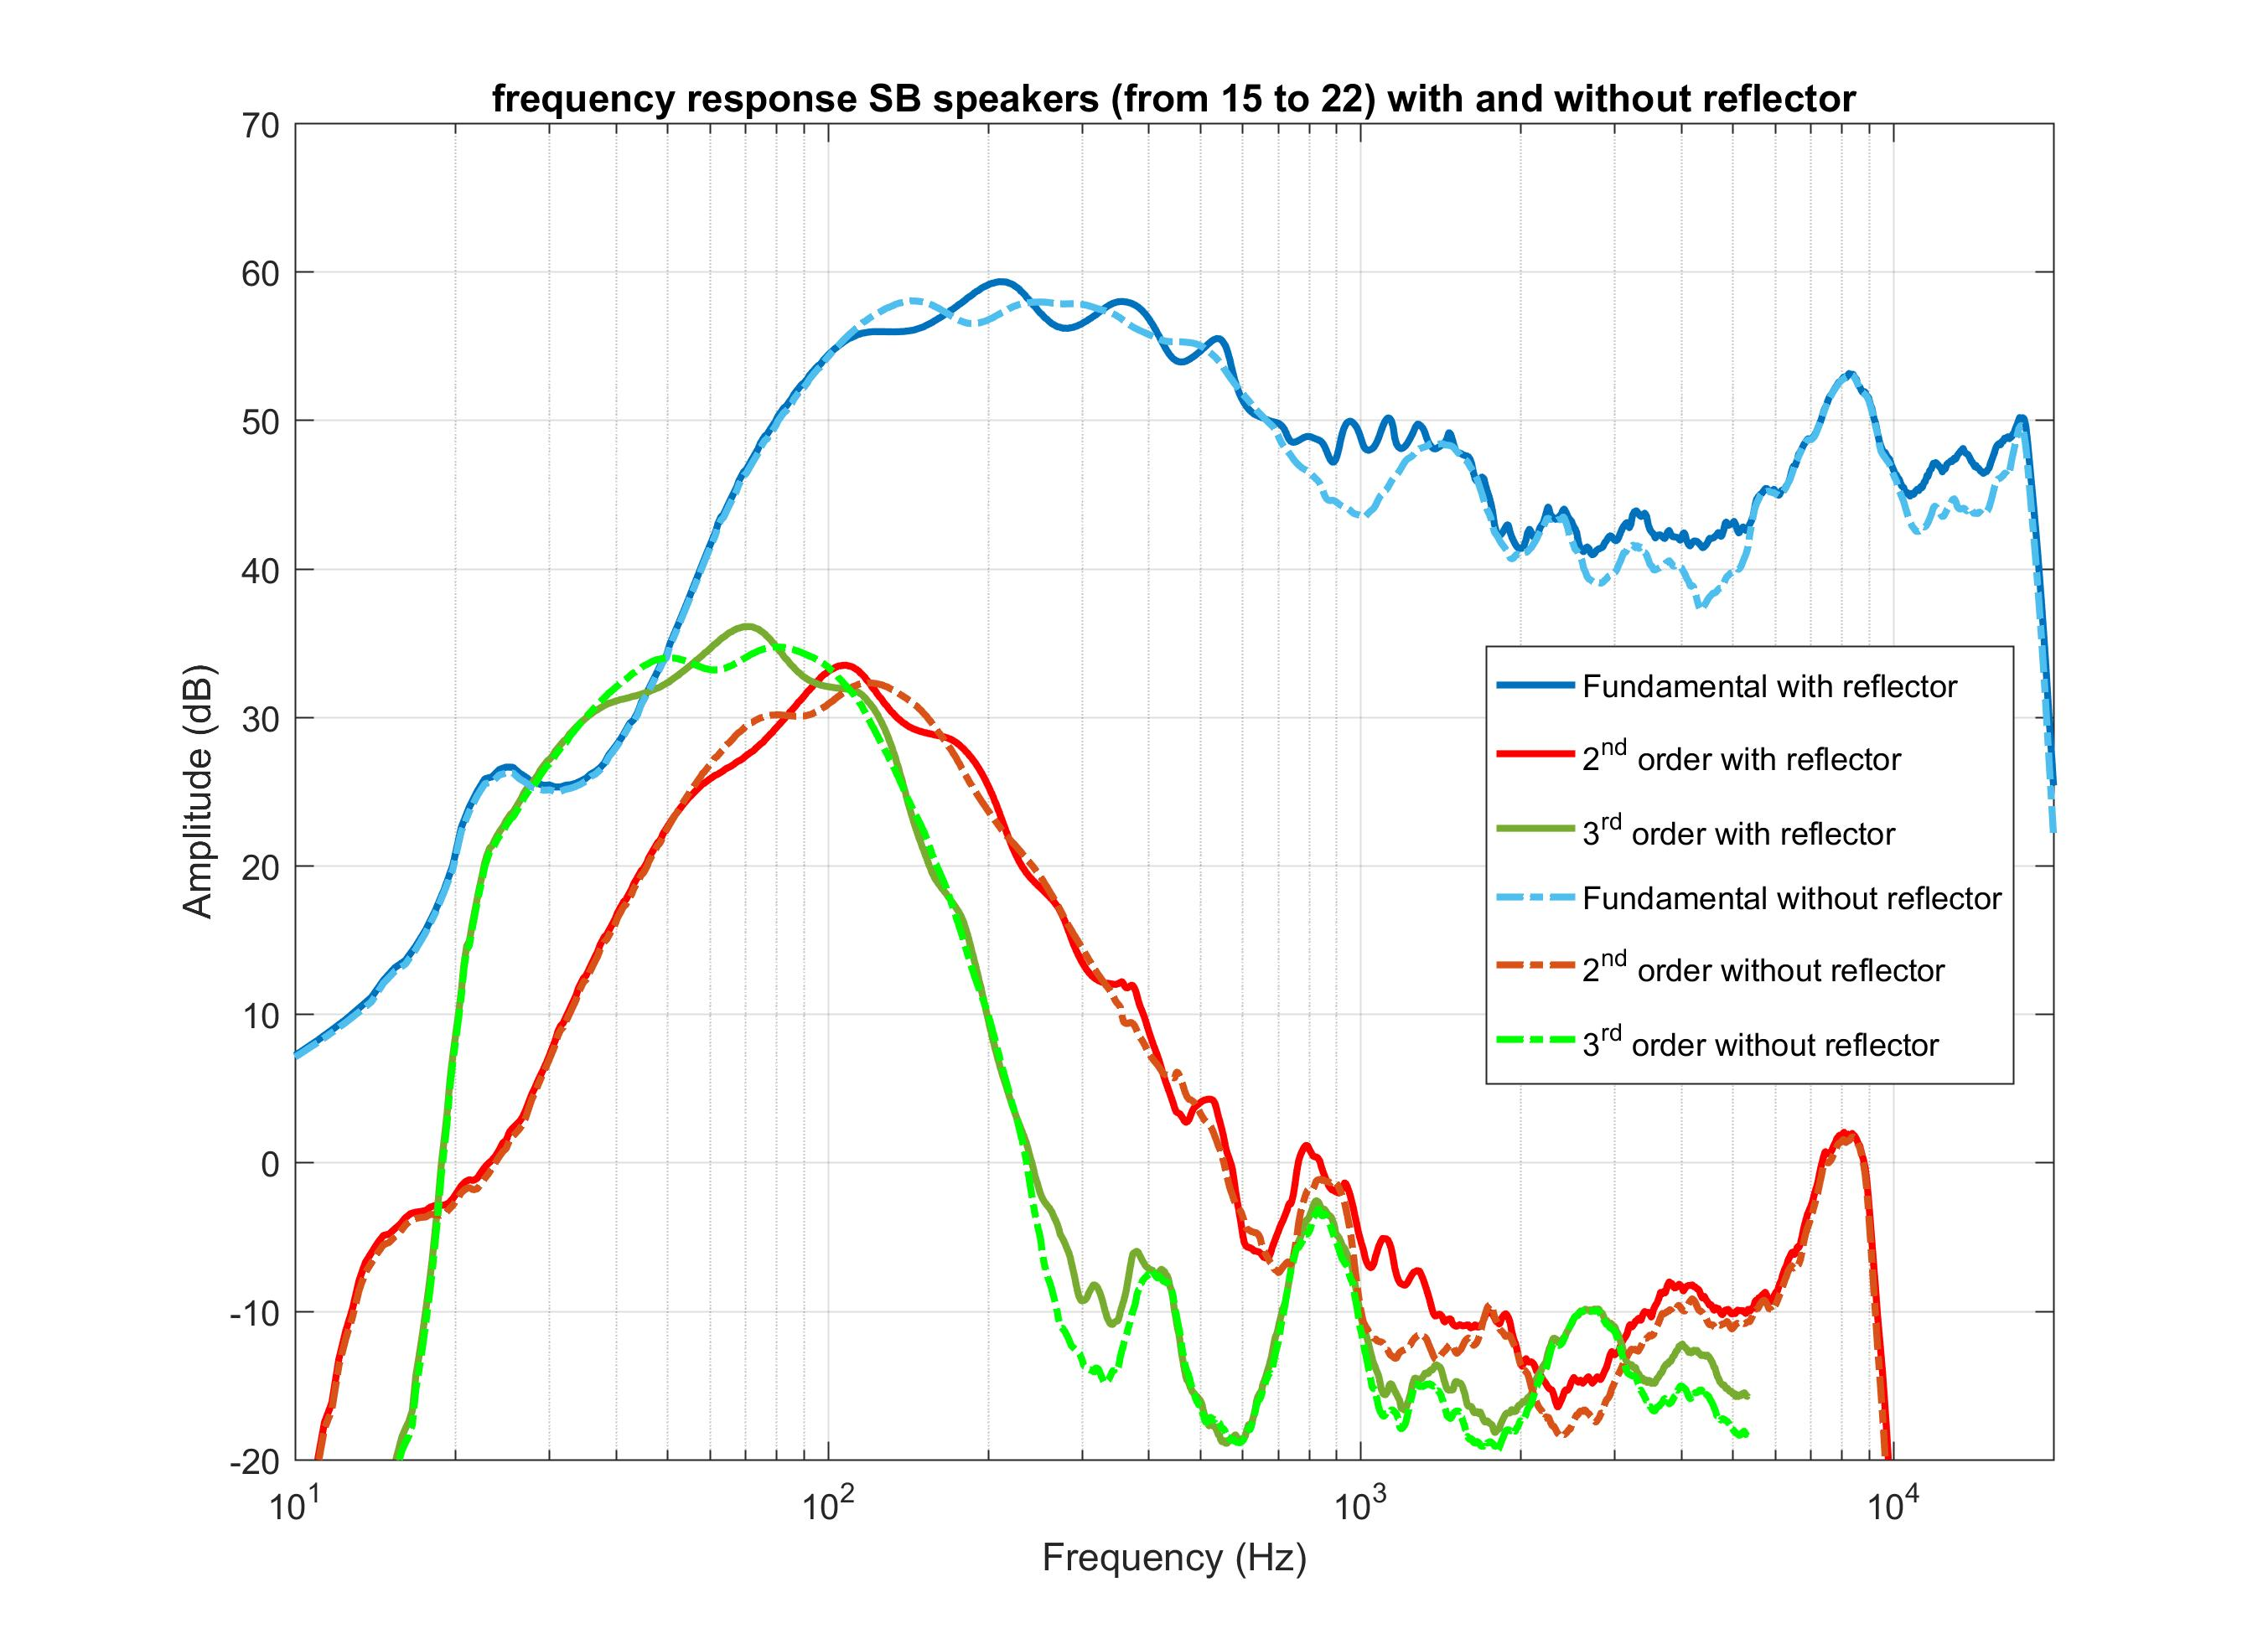
\includegraphics[width=15cm,height=15cm,keepaspectratio]{Figures/sbwithwithoutfreq}
\decoRule
\caption[Frequency response with and without reflector]{Frequency response of the system with (solid lines) and without (dotted lines) reflector.}
\label{fig:freqrespwithwithout}
\end{figure}

It appears that, when the reflector is inside the chamber, the amplitude of the harmonics starts oscillating. This is caused by the standing wave effect. The reflected waves have a certain phase when arriving at the detection point. Depending on the phase value, those have the effect of lowering or increasing the amplitude of the direct wave, since they interfere with each other. As it can be seen from the graph, the magnitude of this phenomena is too weak to cause a significant effect on the frequency response (even though it is clearly visible) and by extension on the ACC filter coefficient estimation.
\\
The $w_{BACC}$ filter calculated with the modified BACC-RD method is presented below. The black box represents a closeup of the second part of the filter. Its ratio is 70:1 with respect of the original scale.

\begin{figure}[H]
\centering
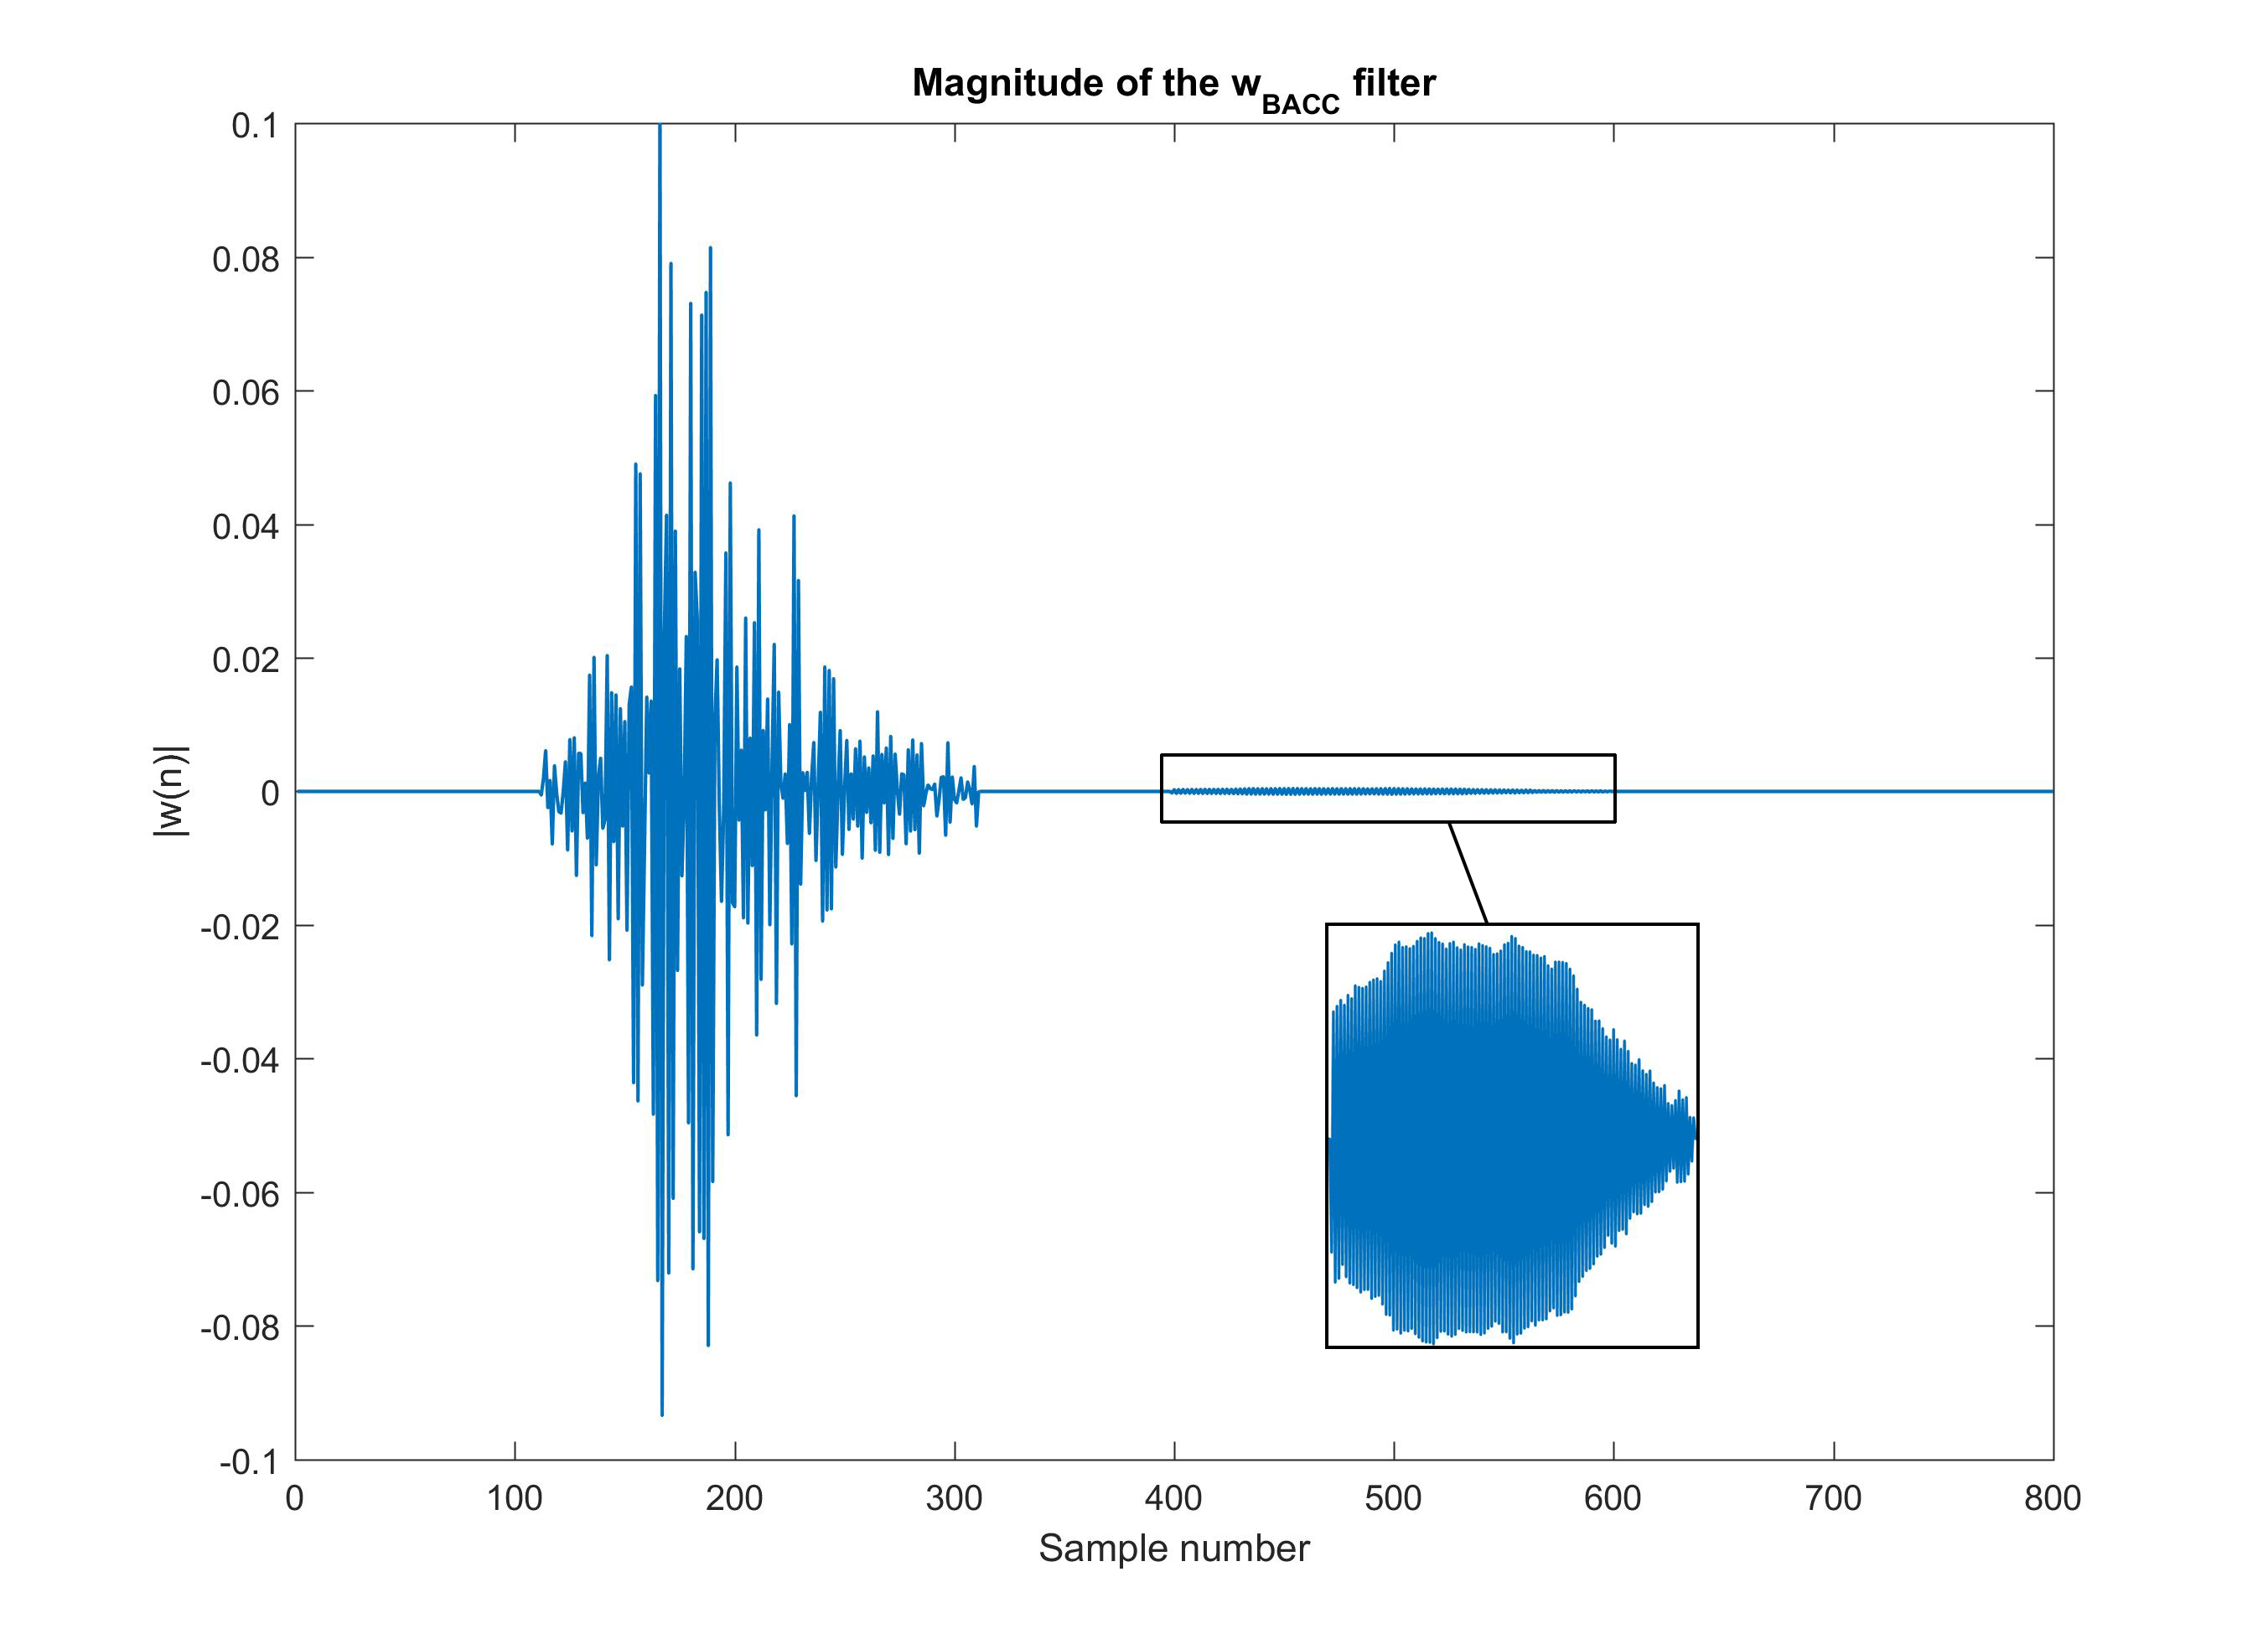
\includegraphics[width=14cm,height=14cm,keepaspectratio]{Figures/filtersplitwithcloseup}
\decoRule
\caption[filter split]{Optimal solution to the Lagrange problem, the black box represents a closeup of the second part of the solution.}
\label{fig:filtersplitwithcloseup}
\end{figure}

As we can see from the final result of the Lagrange problem the part of the filter that contrasts the reflection has an amplitude that is too low compared with the first part of the filter, this is because the energy of the reflected wave itself is too low compared with the one of the direct wave. Nevertheless we can measure the contrast generated by this filter.
\\
\\
Here we can see the frequency response of the system as recorded by microphone $20$. The regularization terms used were $\beta=0.5$, $\delta = 10^{-6}$, an output level of $-35$ and input signal in the $[500-2200]$Hz range. The Contrast figure is $21.8\pm2$dB, obtained by averaging five trials of the experiment.

\begin{figure}[H]
\centering
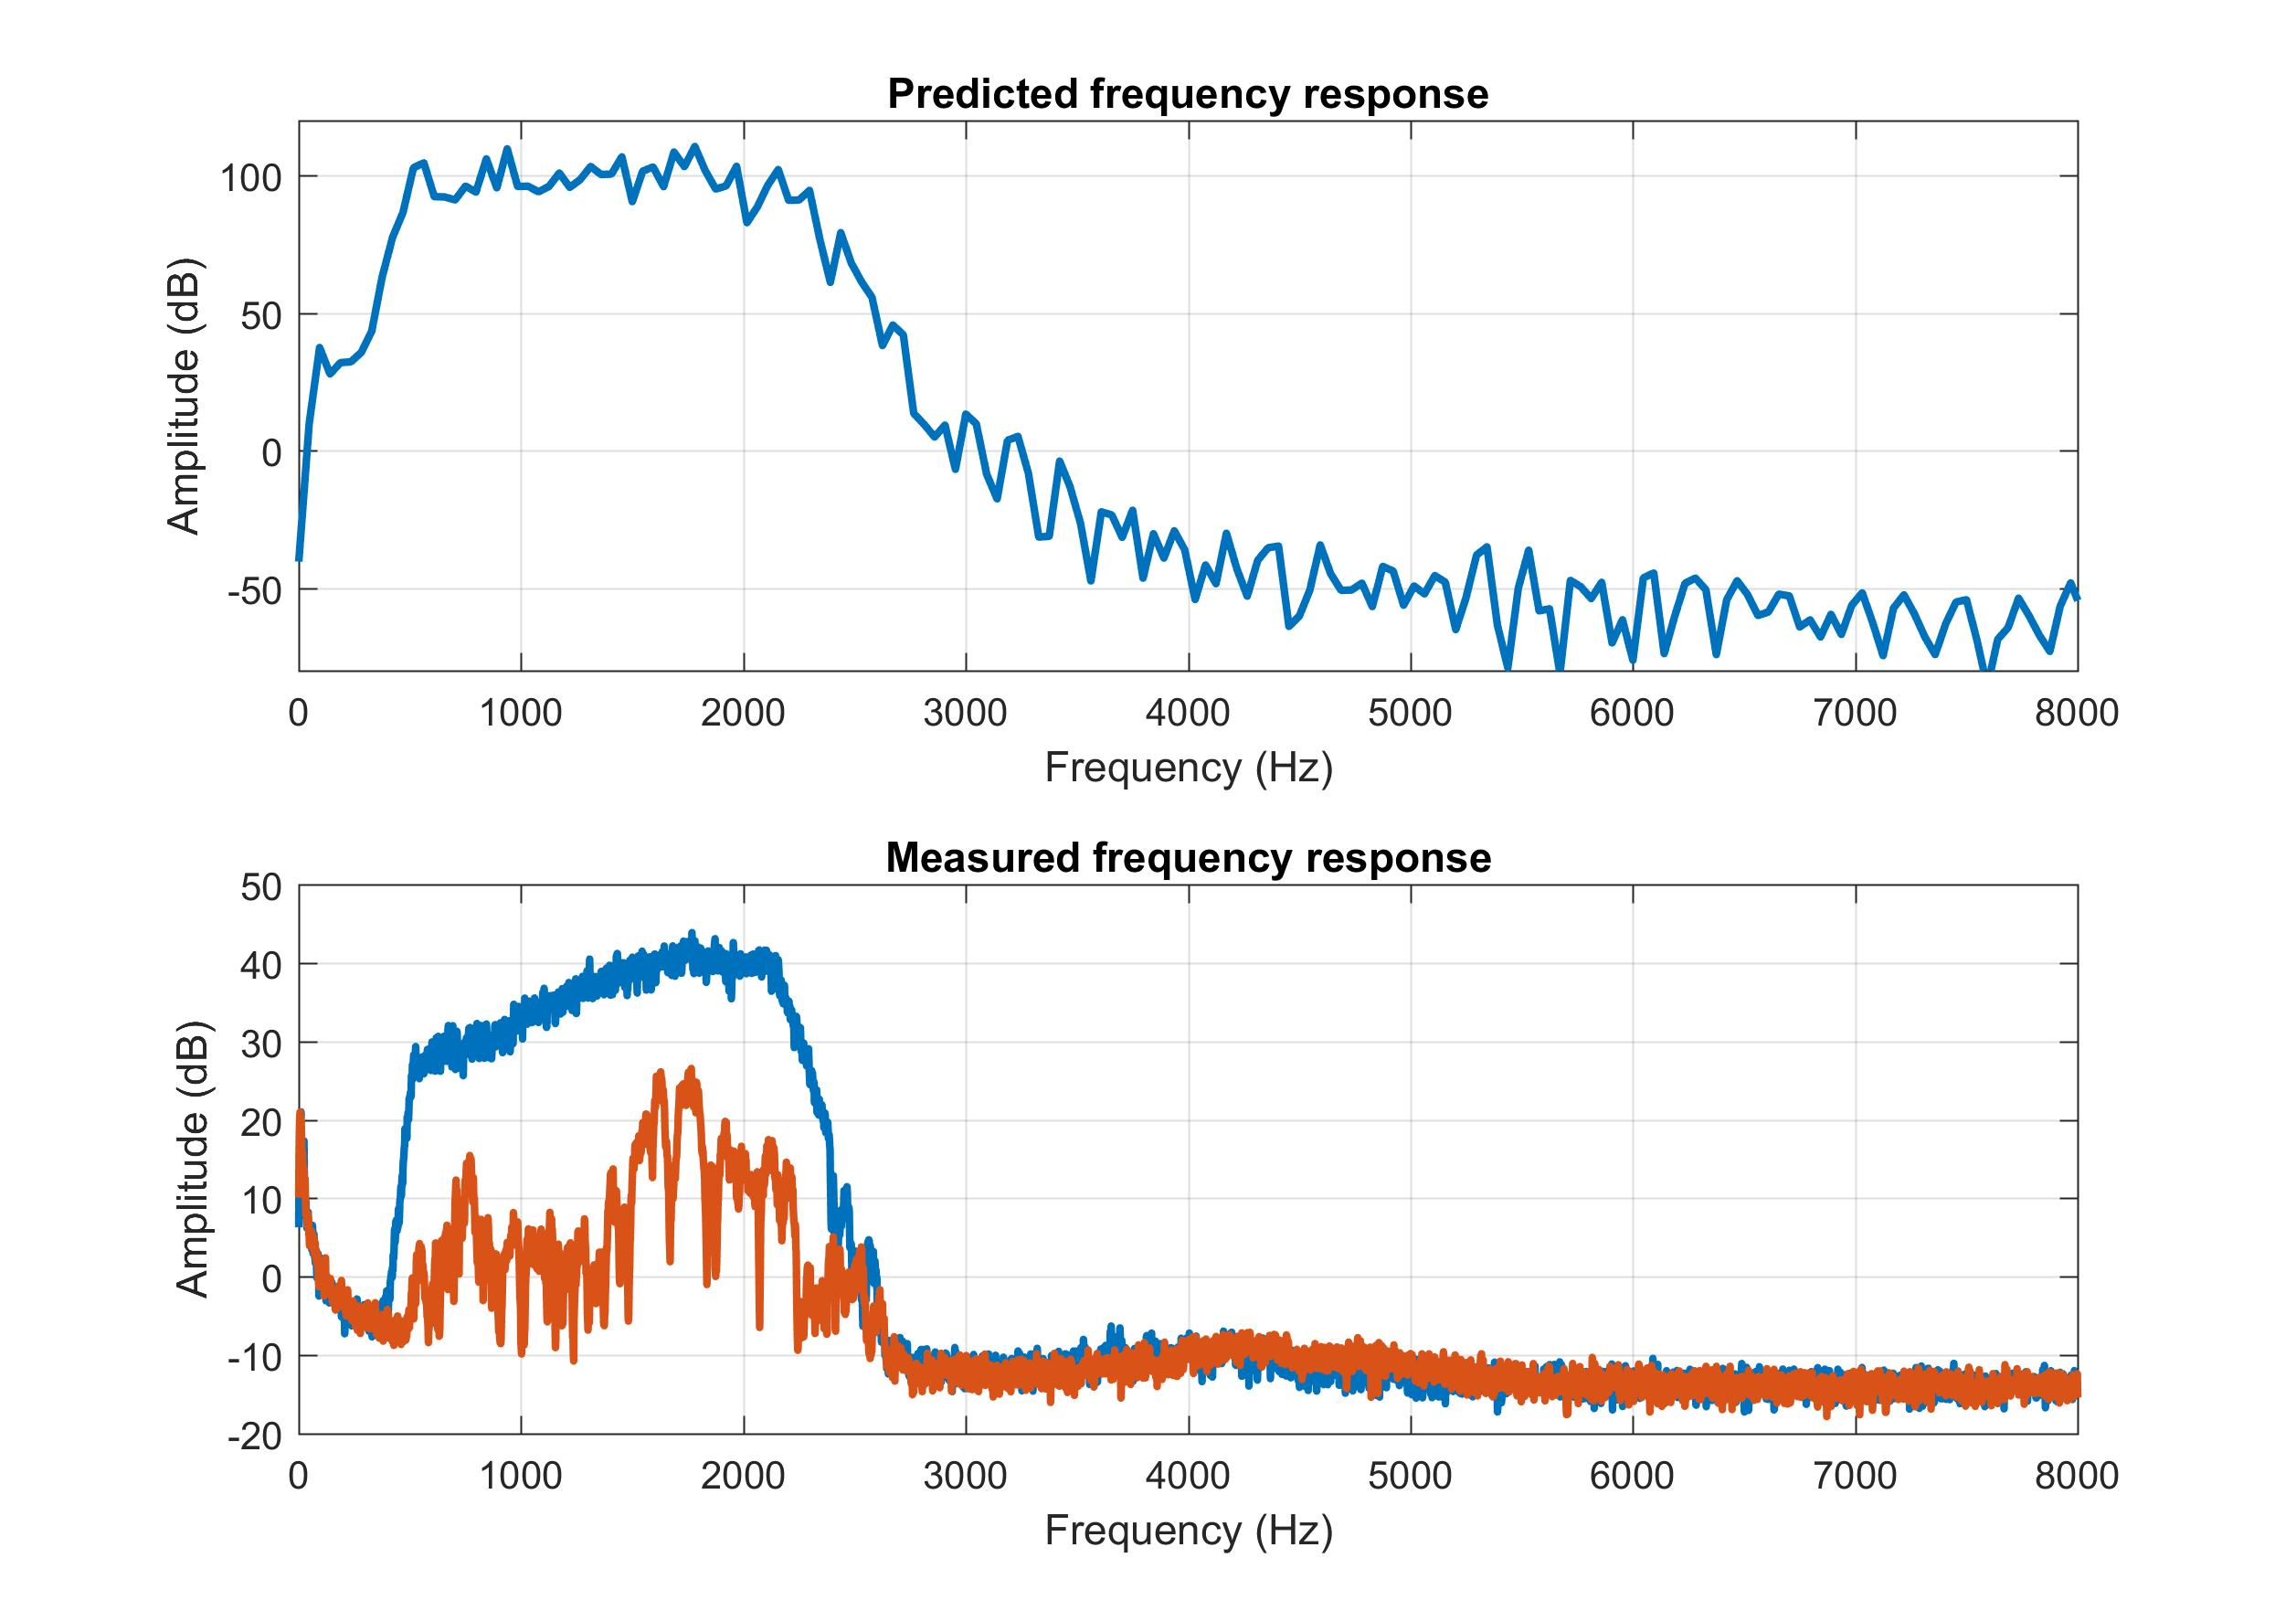
\includegraphics[width=15cm,height=15cm,keepaspectratio]
{Figures/fftbaccsplit}
\decoRule
\caption[Frequency response]{Frequency response of the system when applying the filter in figure \ref{fig:filtersplitwithcloseup}.}
\label{fig:welchfiltersplit}
\end{figure}

The total filter length of 400 samples, divided in two pieces of 200 samples each. The system IR from which the filter was calculated (a cut out of the IR represented in figure \ref{fig:ir_refl_bright}) was 800 samples. The sampling frequency, downsampling rate, microphones and speakers used are the same of the experiment done with a single filter. Is it therefore natural to compare this contrast figure with the one in the experiment \ref{subsec:baccrdanechoic}, an attentive reader will notice the similarity between the spectra of the two graphs (\ref{fig:fr_multiple}).
\\
The contrast figure obtained in that section was $24.5\pm2$dB. The contrast obtained by a BACC filter obtained with the same algorithm of section \ref{subsec:baccrdanechoic}, granted $20.6\pm2$dB, as explained at the beginning of this section. The modified version of the algorithm gives us $21.9\pm2$dB of contrast. It is reminded that all of the measurements have been repeated five times and the results averaged. As we can see the improvement is very modest and generally it has be said that even though encouraging, this solution here proposed requires more studying order to evaluate its efficacy. The algorithm is a good starting point when it comes to tackling the reflection problem in a simplified scenario such as the one used for the experiment.
\\
\\
The reader should be made aware of the shortcomings of the algorithm. First of all, it is clear that the second part of the filter affects the system in a limited way. This is due of the low energy that the reflector adds to the sound zones. One interesting development of this experiment would be to execute the algorithm with a different reflector, possibly one with a more visible effect than the one currently available. Moreover, as previously said, the square window is a suboptimal window function that can affect the system in a negative way.
\\
Due to these limitations it is hard to say that this modified version has a clear beneficial effect to the overall contrast and though it certainly it has not a negative impact in the contrast, more research is needed to study its potential positive effects.


\section{Bacc-RD in the listening room}{}
\label{sec:baccrdlisteningroom}

In the previous section we investigated the characteristics and performances of the BACC-RD algorithm in an anechoic chamber setup and explored a possible modification that can be applied to the concept in a scenario with a single reflector.
\\
Let's now consider a different environment, the listening room. We already presented the setup of the room in section \ref{subsec:mics} and discussed that by its nature, this scenario it's much more difficult to control, since there asre many surfaces that scatter the sound energy everywhere.
The figure below shows the impulse response of the room in question

\begin{figure}[H]
\centering
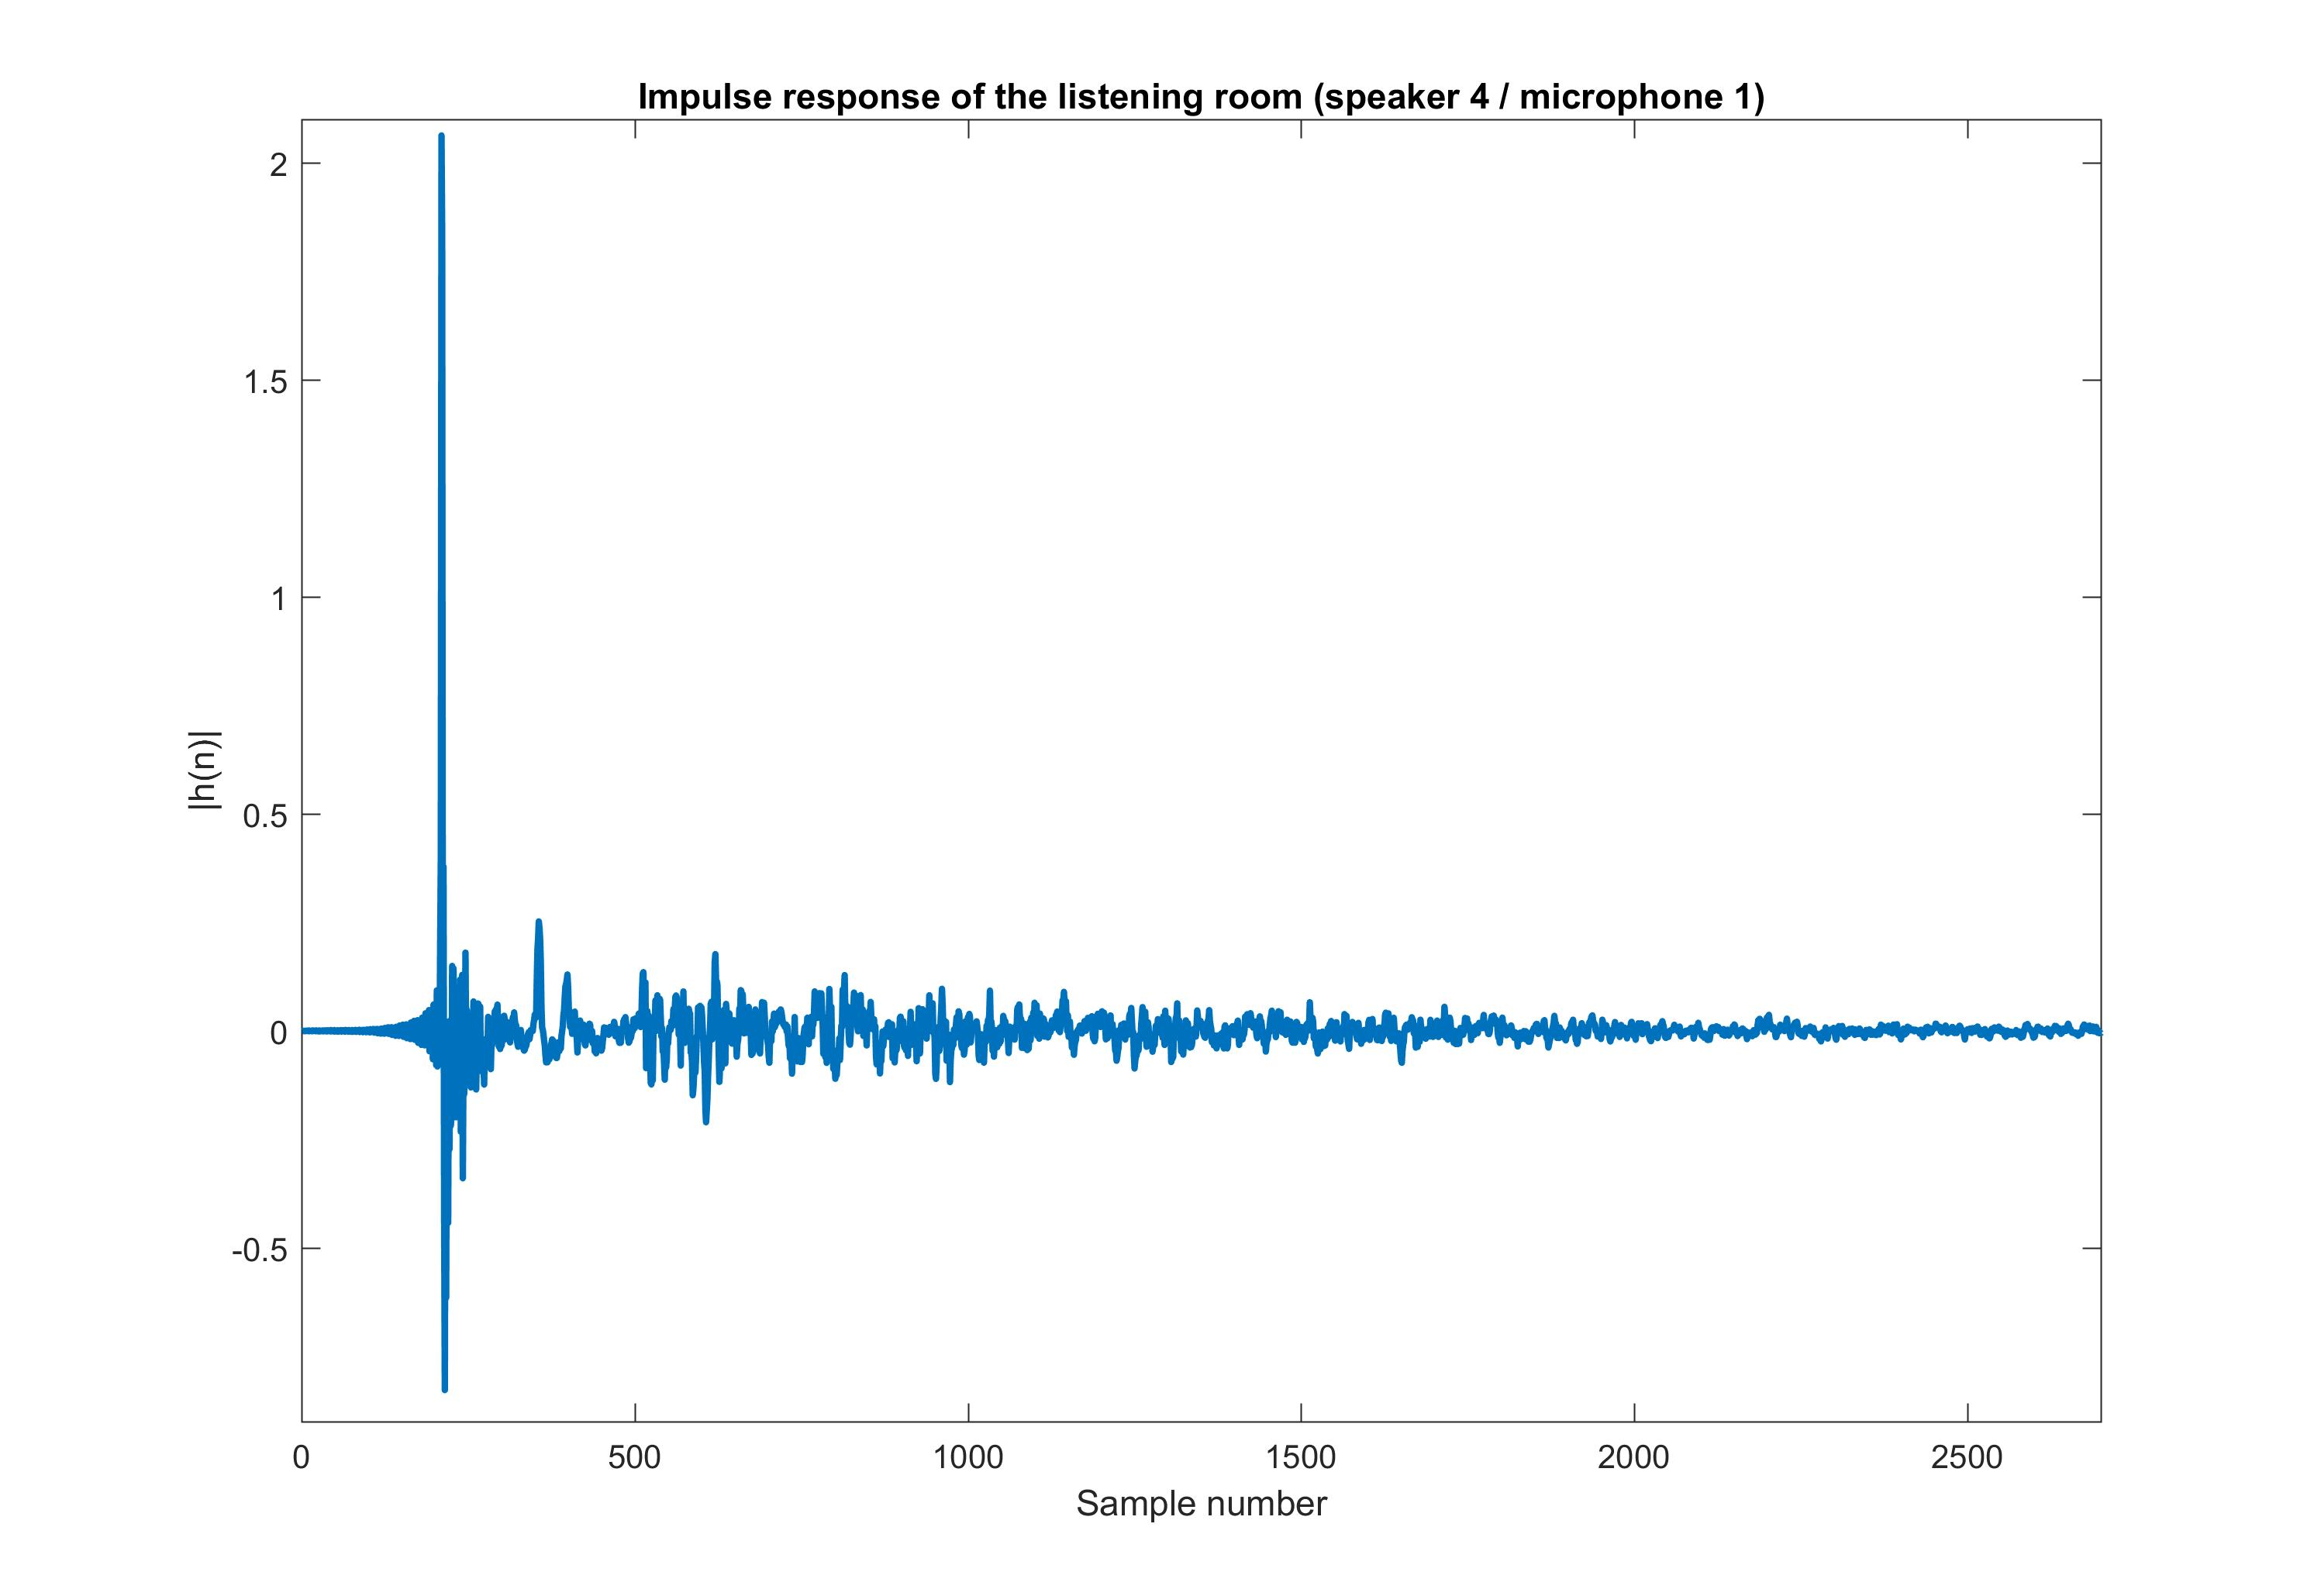
\includegraphics[width=15cm,height=15cm,keepaspectratio]
{Figures/irlisteningroom}
\caption[IR listening room]{Impulse response of the listening room detected in the bright zone.}
\label{fig:irlisteningroom}
\end{figure}

As we can see, in order to represent the system effectively, we need many samples of the IR. Since this introduces unacceptable computing times, especially for the $R_b, R_d$ terms in equation\ref{eqn:lagrange}, we need to limit as much as possible the filter length
\\
The room setup is shown in figure \ref{fig:listeningsetup}. While recording the room's impulse response and performing the test I am inside the room.
\\
Using the original filter concept (the one in sections \ref{subsec:baccrdanechoic} and \ref{subsec:baccvary}) we get a contrast figure of $13.1\pm2$dB, using a $400$ taps filter with $\beta = 0.5, \delta = 1\text{x}10^{-6}$ and a frequency band in the $[500-1800]$Hz range.
Some things have to be said for this figure, first of all the actual contrast detected by each microphone has much more variance, meaning that even though the average figure is the one stated above, some microphone show a contrast as low as $10$dB, while other have a contrast of $16.5$dB. This is due the standing wave effect, which, as we already explained, is a phenomena generated when a soundwave that is reflected back to a given position interferes with another wave coming from a different direction, this generates destructive or constructive interferences at some given positions (dependent on the wave length of the waves) called nodes. The resulting wave is generated by a superposition of the two, which means that will have an amplitude, phase and direction which depends by the characteristics of the interfering sounds.
\\
\\
Due to the spatial dependency of the standing wave effect, the individual regularization of the speakers weights ($\beta, \delta$) might once again prove to be beneficial for the contrast figure.
\\
\\
Using the new algorithm with the same parameters ($400$ taps, $\beta = 0.5, \delta = 1\text{x}10^{-6}$) leads to a contrast $15.4\pm2$dB, which is a modest improvement on the result achieved by the original version of BACC-RD. This is given by the fact that the algorithm automatically detects the source that contributes most to the reflections, by calculating the correlation between the logsweep signal before and after being outputted from the speakers.
\\
The following figure presents the frequency response of the system when solicited with the filters discussed above, the first graph shows the FFT of the recorded samples when the original BACC-RD has been used to find the weights vector, while the second shows the performances achieved with the modified algorithm.

\begin{figure}[H]
\centering
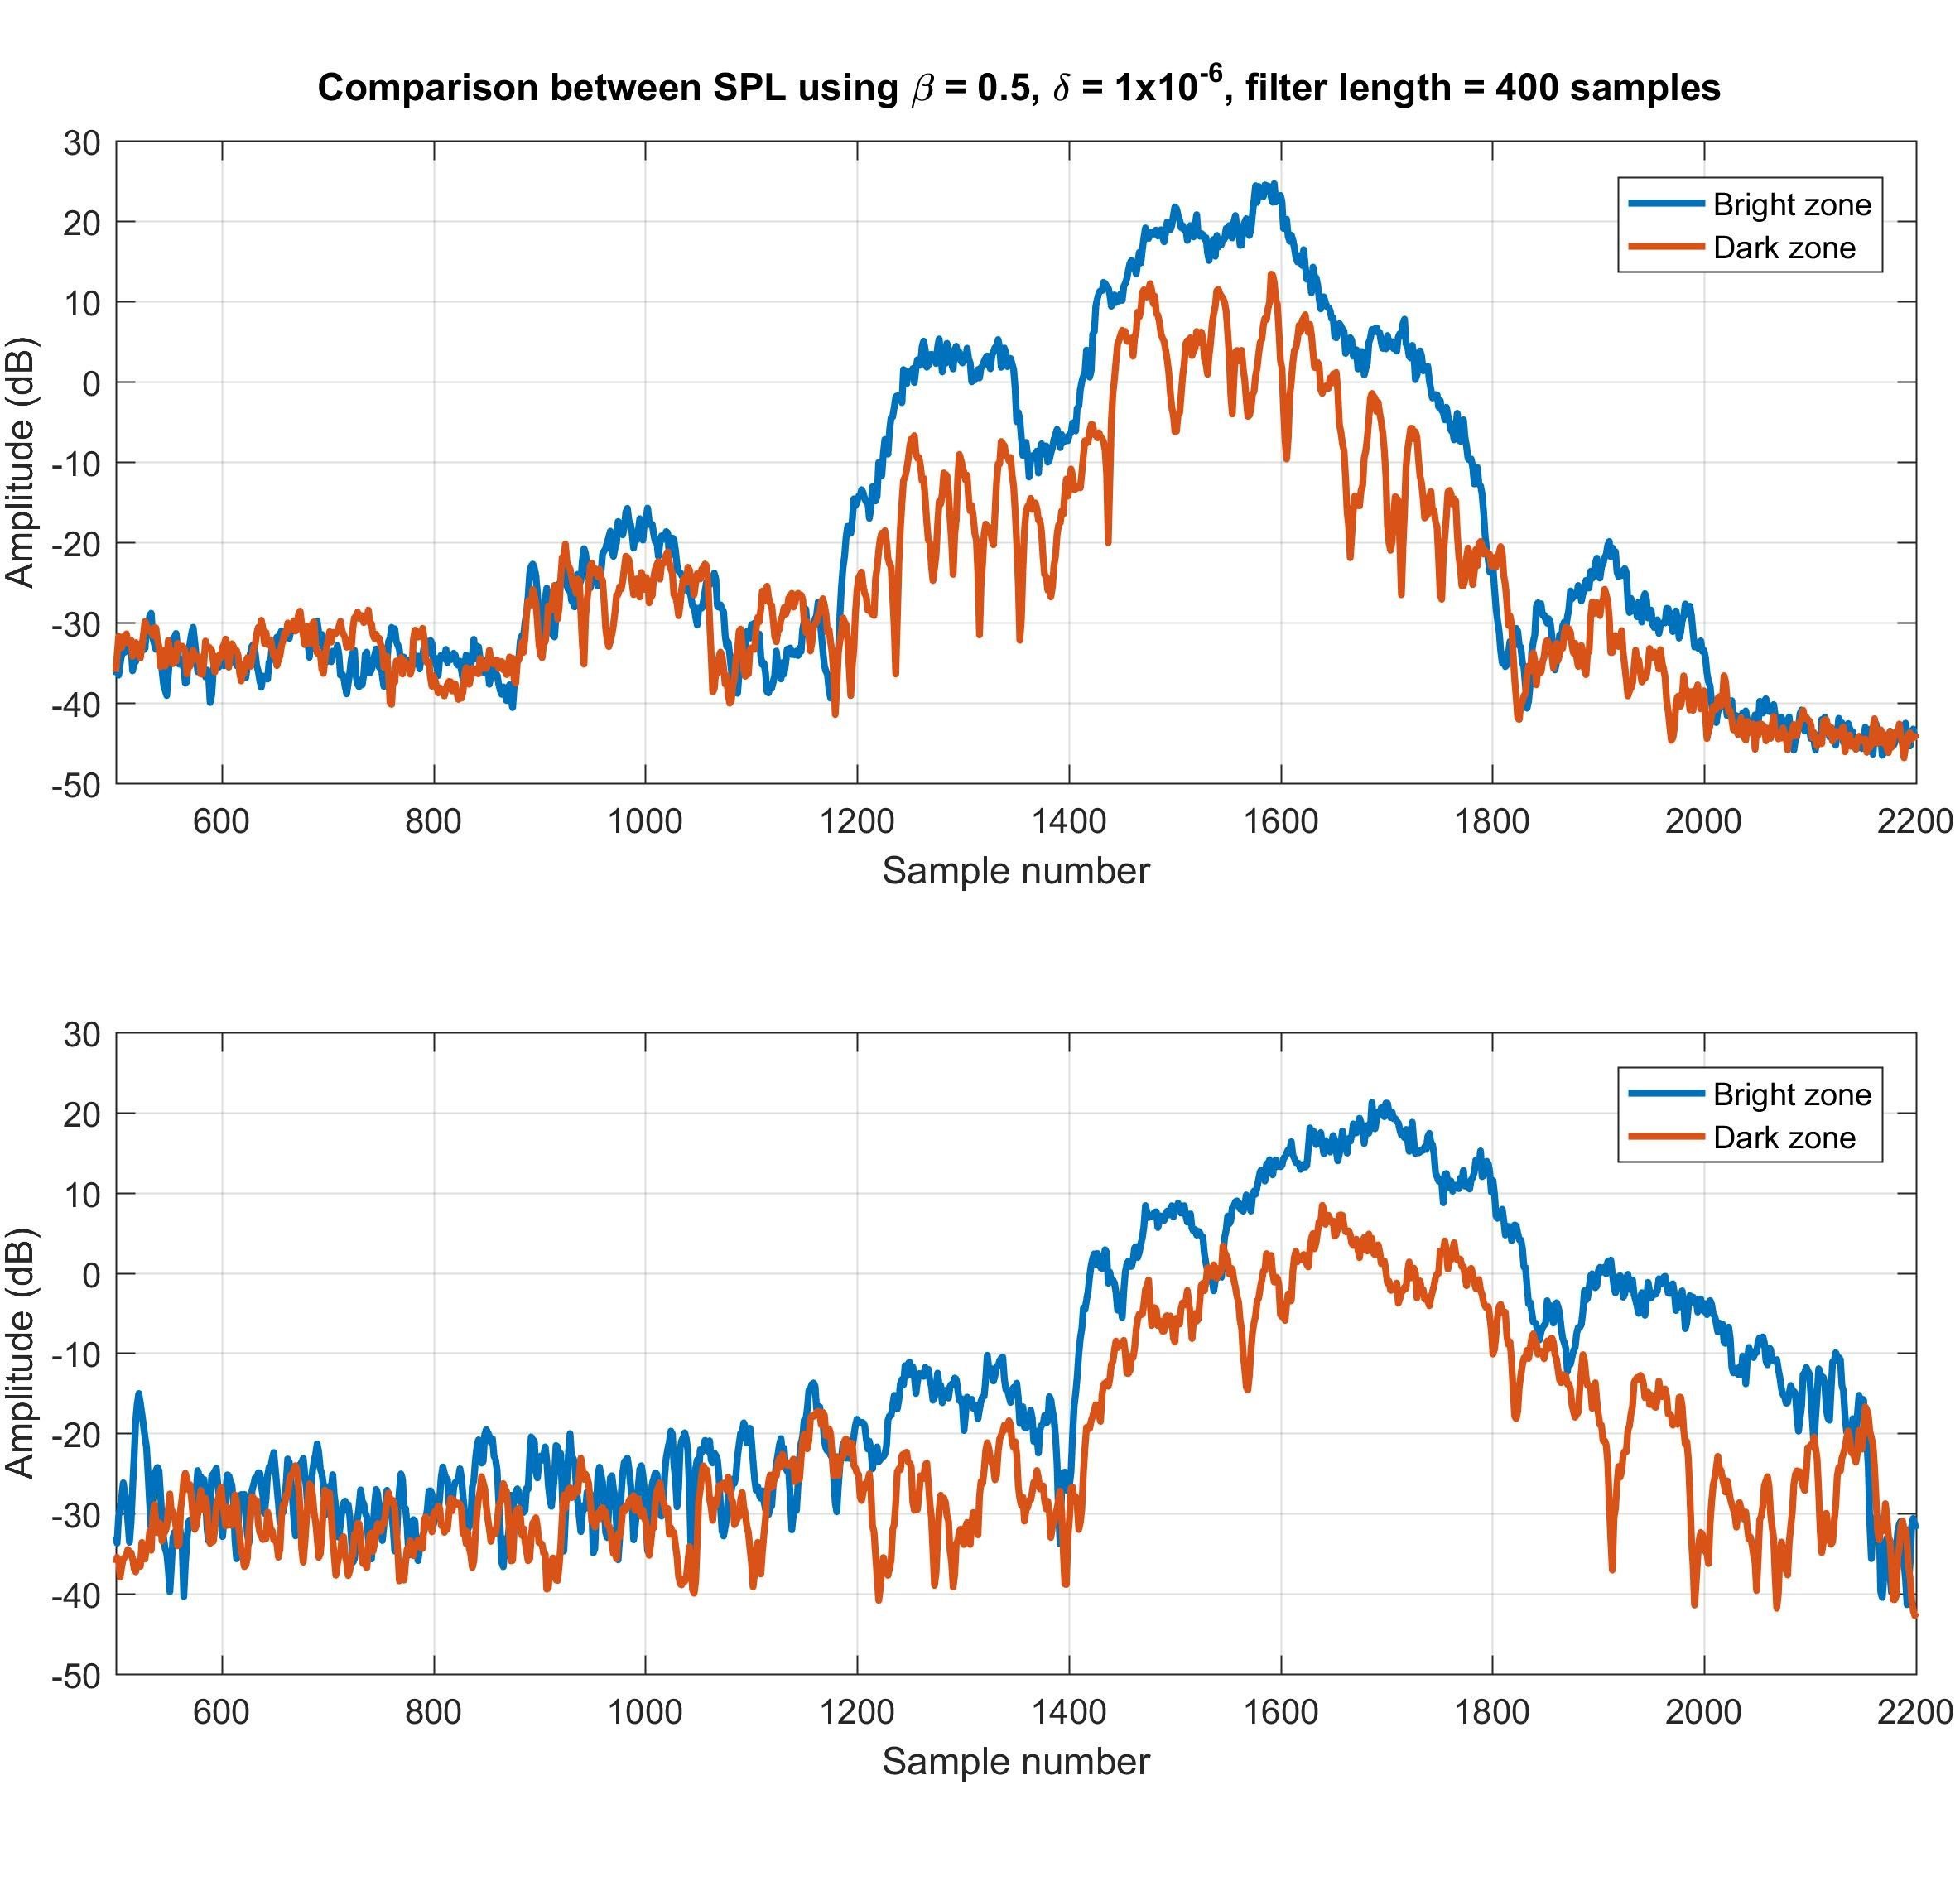
\includegraphics[width=15cm,height=15cm,keepaspectratio]
{Figures/fftfilterslisteningroom}
\decoRule
\caption[FFT listening room]{Fast Fourier Transform of the samples recorded in the listening room using the two verisons of the BACC algorithm.}
\label{fig:fftfilterslisteningroom}
\end{figure}

As we can see the energy is totally concentrated close to the upper frequency limit of the signal. This kind of behavior generates too much distortions of the original sound signal. This graph shows that introducing a new constraint regarding the difference in power level that can be allowed to two adjacent frequency bands seems to be even more beneficial in this kind of environment than the one of the anechoic chamber.
\\
We can also see how the signal, once convolved with the filter, loses almost all its lower frequency content, which doesn't reach the $0$dB mark before $1400$Hz. This kind of behavior is justifiable by the fact that having short filter length means that the algorithm is more capable of controlling only the higher frequencies, for instance, since we have a $400$ taps filter (in the first graph) and a sampling frequency of $4800$Hz the theoretical limit that can be controlled is $\frac{4800}{400}=12$Hz. In the second case we have an even higher theoretical limit, since we split the IR (and the filter) in two parts of $200$ taps each. We can in fact see how the modified algorithm (in the second graph) "pushes" the signal to the higher frequencies even more than the first filter.
\\
\\
Increasing the filter length generates an improvement of contrast, in fact, using $500$ taps we have a jump of \tld$2$dB in the contrast figure. In this case, unlike section \ref{subsec:baccvary}, the filter length is an important parameter to take into account, keeping in mind that the computational time greatly increases for longer filters (\tld 6 minutes for a $500$ taps, \tld1 hour for $600$ taps).
The contrast figure of the new algorithm, instead, seems not to scale with increasing the filter length, because the two "pieces" of the filter tend to end up adjacent one another, and at that point the original algorithm is superior because the control frequencies that determine the local maximum of the contrast are more tightly spaced one another, since they depend on the filter length (so they are at half the distance in a $500$ taps filter rather than 2 partial filters with $250$ taps each.
 
\chapter{Conclusions and future works} % Main chapter title

\label{Chapter5} % For referencing the chapter elsewhere, use \ref{Chapter3} 

%----------------------------------------------------------------------------------------
This work focused on finding a suitable method for performing acoustic contrast control and evaluated its performances and limitations, both inherent to the algorithm itself or given by external factor such as the surrounding environment.
\\
The experimental conditions in the anechoic chamber have been defined, by testing the assumptions regarding the non-linear distortions generated by the loudspeakers, as well as the background noise and the free field attenuation, together with the limit introduced by spatial and frequency aliasing. Once the operating environment has been treated, it was possible to analyze the performances of the algorithm at boundary conditions to find limitations, edge cases and opportunities for future improvements.
\\
Successively, a small evolution of the algorithm has been proposed, it tried to tackle the uncertainties introduced by a reflector surface given by the resulting increase in the energy content inside the controlled zones, caused by the redirected soundwaves.
\\
The idea behind the modification proposed was that, if we could separate the contribution given by the direct hit and the reflected hit we could calculate two contrast filters separately, therefore speeding up the calculations with little change to the contrast figure.
\\
The algorithm proposed has limited applicability in a scenario where the reflections can be easily identified in the impulse response and subsequently windowed out. There are still limitations on this approach given by the distortion that the windowing function introduces in the impulse response. Also the analysis of the reflections, even though shows promising results, is limited to a single scenario and provides results that cannot be considered conclusive, mostly due to the poor choice of the reflector used.
\\
Finally the ACC method developed has been tested in a real environment, demonstrating that some acoustic contrast is possible in an highly reflective environment, but its performances are still not satisfying enough to be applied in a day-to-day scenario.
\\
\\
From the experiments some areas of possible improvements can be identified, specifically two modifications show some potential for an improved, future, version of the current algorithm:

\begin{itemize}
\item Introducing single regularization terms ($\beta, \delta$) for each loudspeaker.
\item Limiting the distortion on the frequency response of the system by limiting the difference in SPL between lower and upper frequency limit, in other words, limiting the tilt of the reproduced signal towards the higher frequency bands.
\end{itemize}

Introducing single regularization terms distributes the control effort more evenly towards all the speakers, generating a more pleasant experience for a potential listener.
\\
The predilection of the BACC-RD algorithm towards the higher frequencies is a problem already observed by \parencite{schellekens_time_2016} which proposes a modification (called BACC-RTE), which limits the mean variation between two adjacent control frequencies by introducing an additional constraint to the maximization problem \ref{eqn:optimization}, thus limiting the skewing effect. The performances of this algorithm look promising and together with the introduction of individual regularization might finally provide satisfying results even in an highly reflective environment.
\\
This is because the reflections introduces standing wave effects. 
These are highly spatially sensitive phenomena, meaning that even a small variation in the position of the speakers might eliminate this phenomena, this can be done by simply penalizing the control effort provided by a speaker (therefore limiting its output) to the advantage of another situated in a more convenient position.
\\
\\
This kind of improvements is left as a suggestion for future works that might follow. 

%----------------------------------------------------------------------------------------
%	THESIS CONTENT - APPENDICES
%----------------------------------------------------------------------------------------

\appendix % Cue to tell LaTeX that the following "chapters" are Appendices

% Include the appendices of the thesis as separate files from the Appendices folder
% Uncomment the lines as you write the Appendices

%% Appendix A

\chapter{Appendix A} % Main appendix title

\label{AppendixA} % For referencing this appendix elsewhere, use \ref{AppendixA}


% \begin{figure}[th]
% \centering
% \includegraphics[width=16cm,height=8cm,keepaspectratio]{Figures/simfreqz}
% \decoRule
% \caption[Simulated IR]{Simulated frequency and phase response. The phase of the system is set to unwrap.}
% \label{fig:simfreqz}
% \end{figure}

% \begin{figure}[H]
% \centering
% 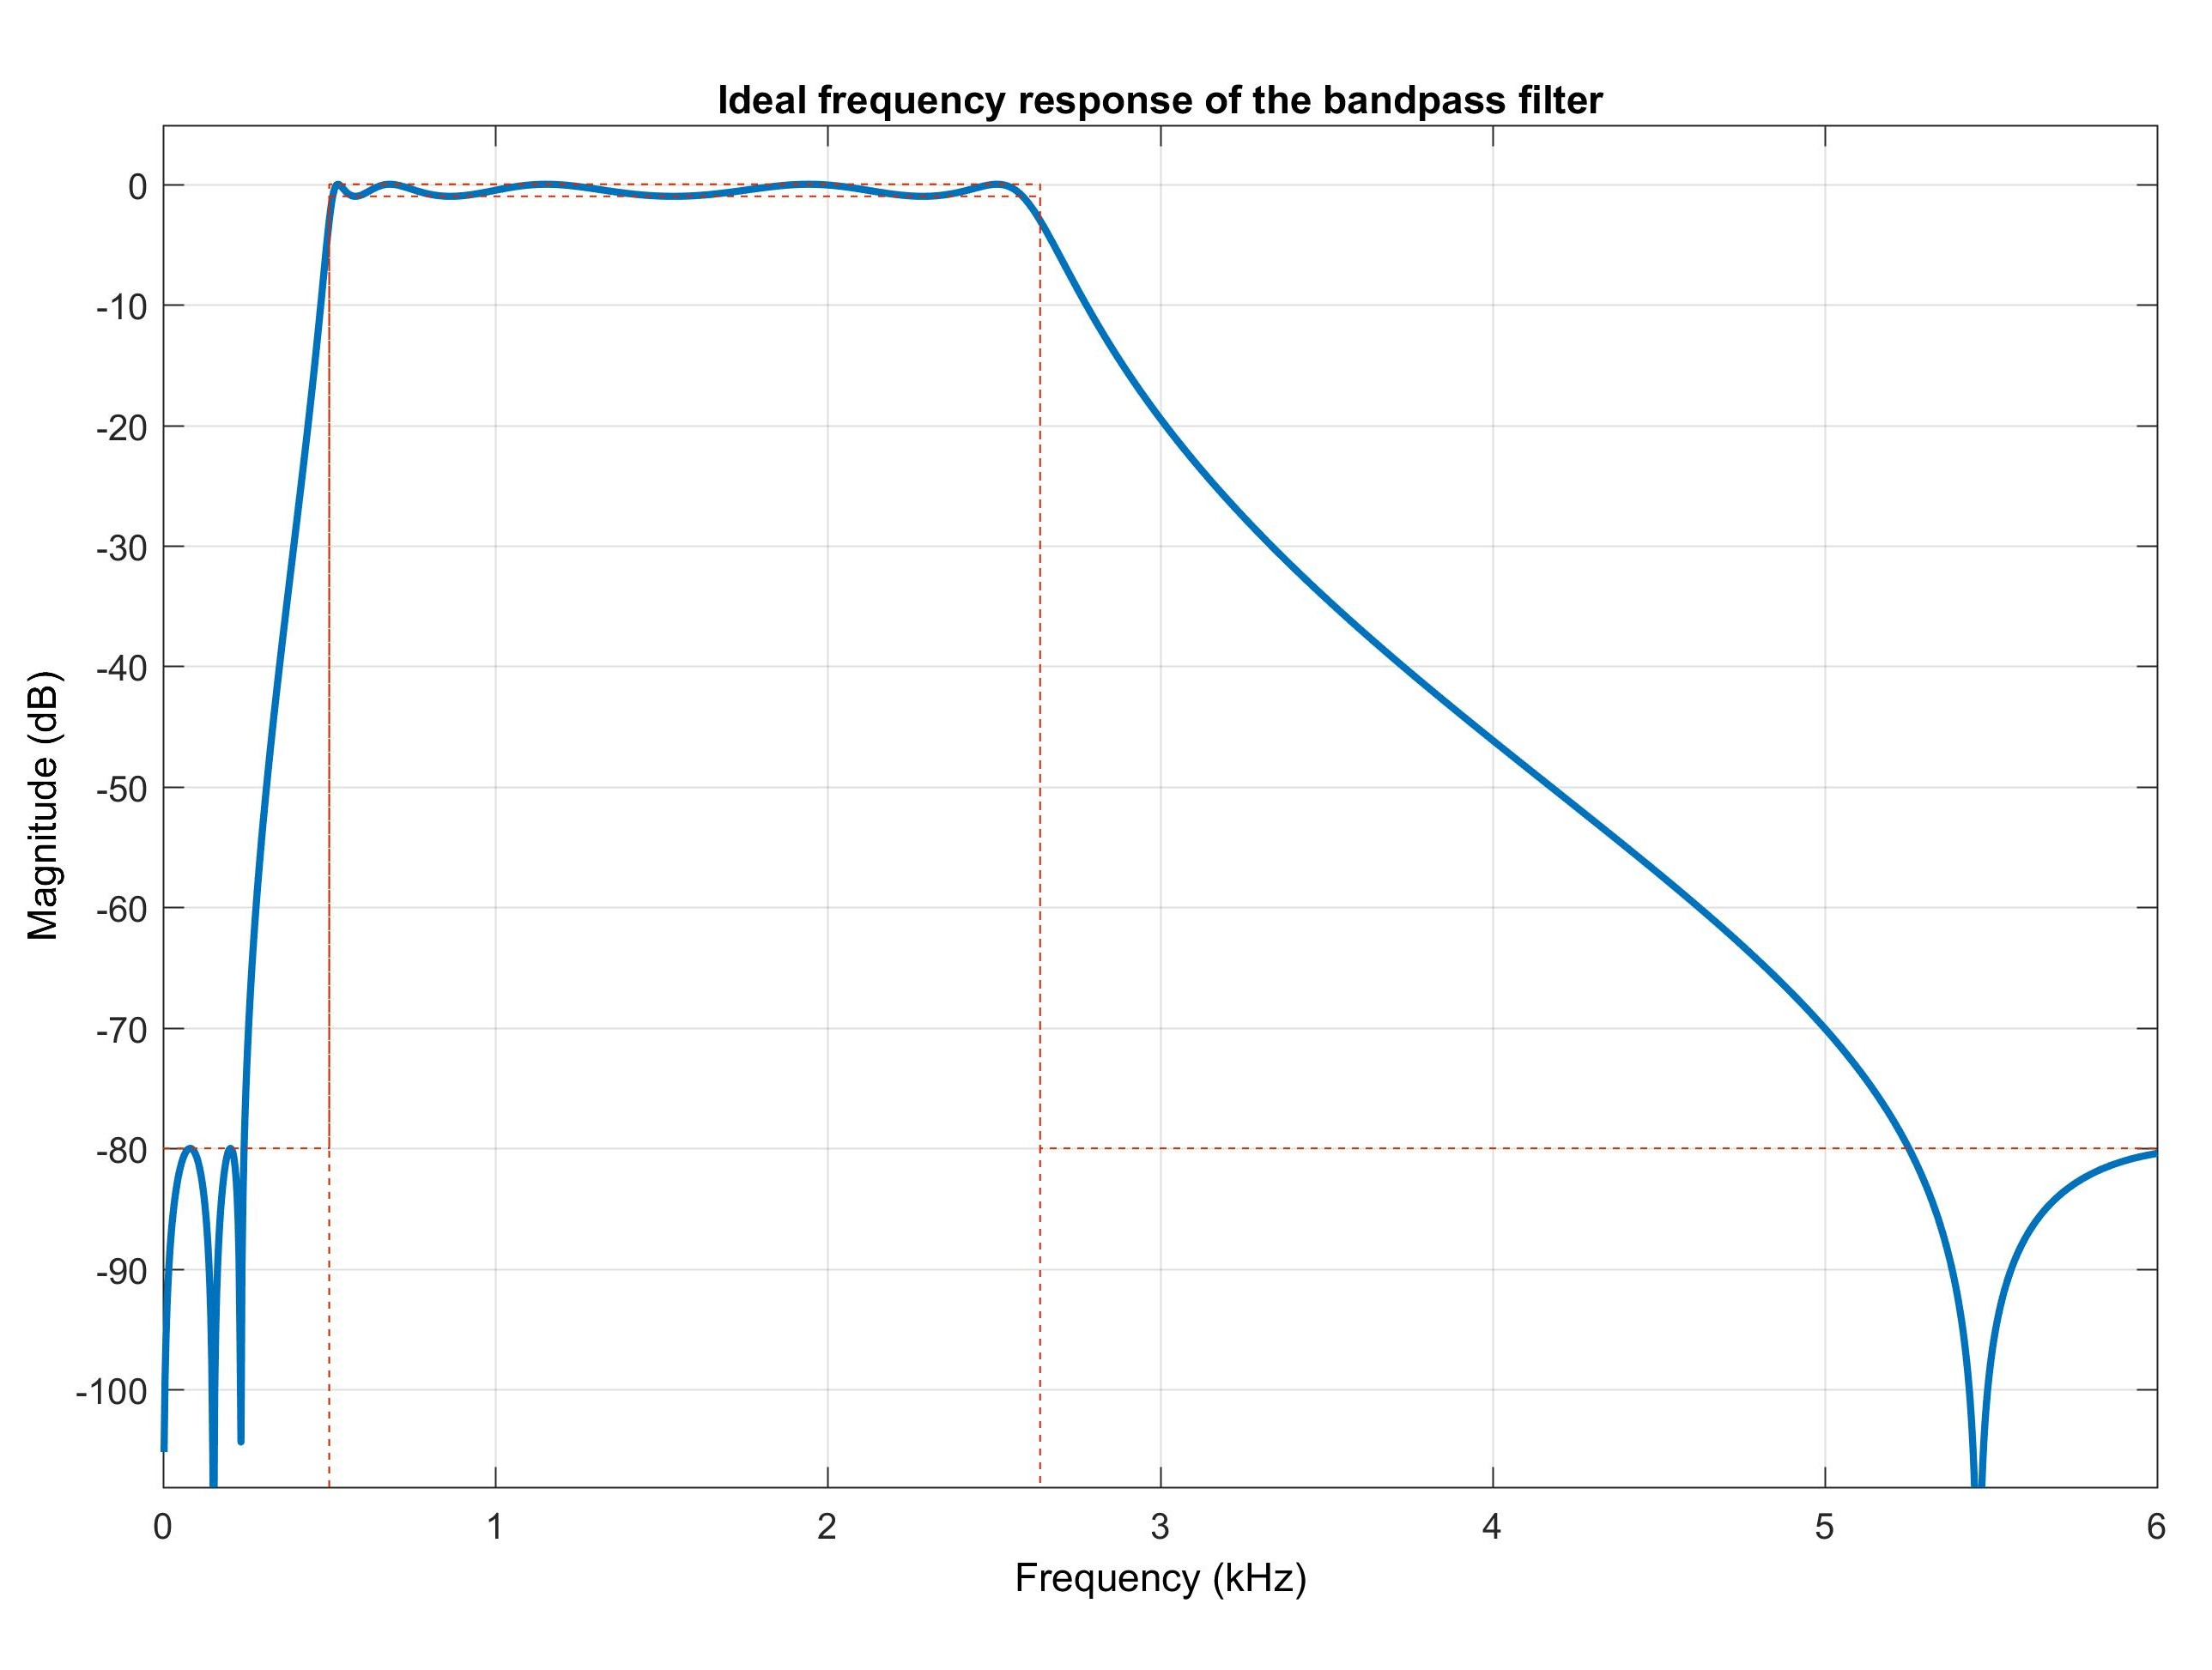
\includegraphics[width=15cm,height=15cm,keepaspectratio]{Figures/noise_bandpass}
% \decoRule
% \caption[Signal bandpass filter]{Test signal bandpass filter }
% \label{fig:noise_bandpass}
% \end{figure}
%\include{Appendices/AppendixB}
%\include{Appendices/AppendixC}

%----------------------------------------------------------------------------------------
%	BIBLIOGRAPHY
%----------------------------------------------------------------------------------------

\printbibliography[heading=bibintoc]
%\bibliography{zotero.bib}

%----------------------------------------------------------------------------------------

\end{document}  
